% Contents from body/page-074.tex.
\BookMark{0}{II  Schemes}{p-74}
\BookMark{1}{2.1  Sheaves}{sec-II-1}
\BeginTypeSheet{74}{60}{}{1}
\Opening{53}{577}{p-74}{II}{Schemes}
\put(53,378){\makebox(0,0)[lt]{\parbox[t]{333.37bp}{%
\normalfont\fontsize{10}{11.5}\selectfont
\setlength{\parindent}{11pt}%
\setlength{\parskip}{1.15pt}%
\noindent This chapter and the next form the technical heart of this book. In this chapter we develop the basic theory of schemes, following Grothendieck \Goto{bib-EGA}{[EGA]}. Sections \Goto{sec-II-1}{1} to \Goto{sec-II-5}{5} are fundamental. They contain a review of sheaf theory (necessary even to define a scheme), then the basic definitions of schemes, morphisms, and coherent sheaves. This is the language that we use for the rest of the book.

Then in Sections \Goto{sec-II-6}{6}, \Goto{sec-II-7}{7}, \Goto{sec-II-8}{8}, we treat some topics which could have been done in the language of varieties, but which are already more convenient to discuss using schemes. For example, the notion of Cartier divisor, and of an invertible sheaf, which belong to the new language, greatly clarify the discussion of Weil divisors and linear systems, which belong to the old language. Then in \Goto{sec-II-8}{\S8}, the systematic use of nonclosed scheme points gives much more flexibility in the discussion of sheaves of differentials and nonsingular varieties, improving the treatment of (I, \Goto{sec-I-5}{\S5}).

In \Goto{sec-II-9}{\S9} we give the definition of a formal scheme, which did not have an analogue in the theory of varieties. It was invented by Grothendieck as a good way of dealing with Zariski's theory of \textquotedblleft{}holomorphic functions,\textquotedblright{} which Zariski regarded as an analogue in abstract algebraic geometry of the holomorphic functions in a neighborhood of a subvariety in the classical case.

\bigskip
\noindent\hypertarget{sec-II-1}{}\textbf{\large 1\quad Sheaves}\par
\smallskip
\noindent The concept of a sheaf provides a systematic way of keeping track of local algebraic data on a topological space. For example, the regular functions on open subsets of a variety, introduced in \Goto{p-15}{Chapter I}, form a sheaf, as we will see shortly. Sheaves are essential in the study of schemes. In fact, we cannot\par
}}}
\EndSheet
% Contents from body/page-075.tex.
\ChapterSheet{75}{61}{\Goto{sec-II-1}{1\quad Sheaves}}{%
\noindent even define a scheme without using sheaves. So we begin this chapter with sheaves. For additional information, see the book of Godement \Goto{bib-godement-1}{[1]}.

\Dfn Let $X$ be a topological space. A \emph{presheaf} $\mathcal F$ of abelian groups on $X$ consists of the data
\begin{enumerate}[label=(\alph*),leftmargin=2.4em,nosep]
\item for every open subset $U\subseteq X$, an abelian group $\mathcal F(U)$, and
\item for every inclusion $V\subseteq U$ of open subsets of $X$, a morphism of abelian groups $\rho_{UV}\colon\mathcal F(U)\to\mathcal F(V)$,
\end{enumerate}
\noindent subject to the conditions
\begin{enumerate}[label=(\arabic*),leftmargin=2.4em,nosep]
\item[\hypertarget{def-II-1-condition-0}{}(0)] $\mathcal F(\varnothing)=0$, where $\varnothing$ is the empty set,
\item $\rho_{UU}$ is the identity map $\mathcal F(U)\to\mathcal F(U)$, and
\item if $W\subseteq V\subseteq U$ are three open subsets, then $\rho_{UW}=\rho_{VW}\circ\rho_{UV}$.
\end{enumerate}

\smallskip
The reader who likes the language of categories may rephrase this definition as follows. For any topological space $X$, we define a category $\mathfrak{Top}(X)$, whose objects are the open subsets of $X$, and where the only morphisms are the inclusion maps. Thus $\operatorname{Hom}(V,U)$ is empty if $V\nsubseteq U$, and $\operatorname{Hom}(V,U)$ has just one element if $V\subseteq U$.
\hypertarget{err-II-1-presheaf}{}\EditionText{With condition \Goto{def-II-1-condition-0}{(0)}, a presheaf is a contravariant functor from $\mathfrak{Top}(X)$ to $\mathfrak{Ab}$ which sends $\varnothing$ to the zero group.}

\EditionText{For the analogous normalized definition with values in a category $\mathfrak C$ with a terminal object, require the value at $\varnothing$ to be terminal in $\mathfrak C$. In particular the terminal objects are the zero ring for rings and a singleton for sets.} We will stick to the case of abelian groups in this section, and let the reader make the necessary modifications for the case of rings, sets, etc.

As a matter of terminology, if $\mathcal F$ is a presheaf on $X$, we refer to $\mathcal F(U)$ as the \emph{sections} of the presheaf $\mathcal F$ over the open set $U$, and we sometimes use the notation $\Gamma(U,\mathcal F)$ to denote the group $\mathcal F(U)$. We call the maps $\rho_{UV}$ \emph{restriction} maps, and we sometimes write $s|_V$ instead of $\rho_{UV}(s)$, if $s\in\mathcal F(U)$.

\smallskip
A sheaf is roughly speaking a presheaf whose sections are determined by local data. To be precise, we give the following definition.

\Dfn A presheaf $\mathcal F$ on a topological space $X$ is a \emph{sheaf} if it satisfies the following supplementary conditions:
\begin{enumerate}[label=(\arabic*),leftmargin=2.4em,nosep]
\item[\hypertarget{def-II-1-condition-3}{}(3)] if $U$ is an open set, if $\{V_i\}$ is an open covering of $U$, and if $s\in\mathcal F(U)$ is an element such that $s|_{V_i}=0$ for all $i$, then $s=0$;
\item[\hypertarget{def-II-1-condition-4}{}(4)] if $U$ is an open set, if $\{V_i\}$ is an open covering of $U$, and if we have elements $s_i\in\mathcal F(V_i)$ for each $i$, with the property that for each $i,j$, $s_i|_{V_i\cap V_j}=s_j|_{V_i\cap V_j}$, then there is an element $s\in\mathcal F(U)$ such that $s|_{V_i}=s_i$ for each $i$. (Note condition \Goto{def-II-1-condition-3}{(3)} implies that $s$ is unique.)
\end{enumerate}

\medskip
\emph{Note.} According to our definition, a sheaf is a presheaf satisfying certain extra conditions. This is equivalent to the definition found in some other
}
% Contents from body/page-076.tex.
\ChapterSheet{76}{62}{\Goto{p-74}{II\quad Schemes}}{%
\noindent books, of a sheaf as a topological space over $X$ with certain properties (Ex.~\Goto{ex-II-1.13}{1.13}).

\smallskip
\noindent\hypertarget{result-II-1.0.1}{}\textbf{Example 1.0.1.} Let $X$ be a variety over the field $k$. For each open set $U\subseteq X$, let $\mathcal O(U)$ be the ring of regular functions from $U$ to $k$, and for each $V\subseteq U$, let $\rho_{UV}\colon\mathcal O(U)\to\mathcal O(V)$ be the restriction map (in the usual sense). Then $\mathcal O$ is a sheaf of rings on $X$. It is clear that it is a presheaf of rings. To verify the conditions \Goto{def-II-1-condition-3}{(3)} and \Goto{def-II-1-condition-4}{(4)}, we note that a function which is $0$ locally is $0$, and a function which is regular locally is regular, because of the definition of regular function (I, \Goto{sec-I-3}{\S3}). We call $\mathcal O$ the \emph{sheaf of regular functions} on $X$.

\smallskip
\noindent\hypertarget{result-II-1.0.2}{}\textbf{Example 1.0.2.} In the same way, one can define the sheaf of continuous real-valued functions on any topological space, or the sheaf of differentiable functions on a differentiable manifold, or the sheaf of holomorphic functions on a complex manifold.

\smallskip
\noindent\hypertarget{result-II-1.0.3}{}\textbf{Example 1.0.3.} Let $X$ be a topological space, and $A$ an abelian group. We define the \emph{constant sheaf} $\mathcal A$ on $X$ determined by $A$ as follows. Give $A$ the discrete topology, and for any open set $U\subseteq X$, let $\mathcal A(U)$ be the group of all continuous maps of $U$ into $A$. Then with the usual restriction maps, we obtain a sheaf $\mathcal A$. Note that for \hypertarget{err-II-1-0-3}{}\EditionText{every nonempty connected open set $U$}, $\mathcal A(U)\cong A$, whence the name \textquotedblleft{}constant sheaf.\textquotedblright{} If $U$ is an open set whose connected components are open (which is always true on a locally connected topological space), then $\mathcal A(U)$ is a direct product of copies of $A$, one for each connected component of $U$.

\Dfn If $\mathcal F$ is a presheaf on $X$, and if $P$ is a point of $X$, we define the \emph{stalk} $\mathcal F_P$ of $\mathcal F$ at $P$ to be the direct limit of the groups $\mathcal F(U)$ for all open sets $U$ containing $P$, via the restriction maps $\rho$.

\smallskip
Thus an element of $\mathcal F_P$ is represented by a pair $\langle U,s\rangle$, where $U$ is an open neighborhood of $P$, and $s$ is an element of $\mathcal F(U)$. Two such pairs $\langle U,s\rangle$ and $\langle V,t\rangle$ define the same element of $\mathcal F_P$ if and only if there is an open neighborhood $W$ of $P$ with $W\subseteq U\cap V$, such that $s|_W=t|_W$. Thus we may speak of elements of the stalk $\mathcal F_P$ as \emph{germs} of sections of $\mathcal F$ at the point $P$. In the case of a variety $X$ and its sheaf of regular functions $\mathcal O$, the stalk $\mathcal O_P$ at a point $P$ is just the local ring of $P$ on $X$, which was defined in (I, \Goto{sec-I-3}{\S3}).

\Dfn If $\mathcal F$ and $\mathcal G$ are presheaves on $X$, a \emph{morphism} $\varphi\colon\mathcal F\to\mathcal G$ consists of a morphism of abelian groups $\varphi(U)\colon\mathcal F(U)\to\mathcal G(U)$ for each open set $U$, such that whenever $V\subseteq U$ is an inclusion, the diagram
\[
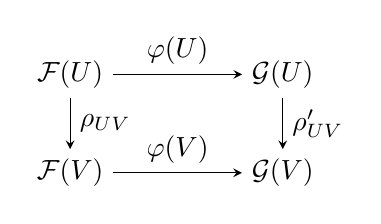
\begin{tikzpicture}[x=1cm,y=1cm,>=stealth]
\node (fu) at (0,0) {$\mathcal F(U)$};
\node (gu) at (2.7,0) {$\mathcal G(U)$};
\node (fv) at (0,-1.25) {$\mathcal F(V)$};
\node (gv) at (2.7,-1.25) {$\mathcal G(V)$};
\draw[->] (fu) -- node[above] {$\varphi(U)$} (gu);
\draw[->] (fv) -- node[above] {$\varphi(V)$} (gv);
\draw[->] (fu) -- node[right] {$\rho_{UV}$} (fv);
\draw[->] (gu) -- node[right] {$\rho'_{UV}$} (gv);
\end{tikzpicture}
\]
}
% Contents from body/page-077.tex.
\ChapterSheet{77}{63}{\Goto{sec-II-1}{1\quad Sheaves}}{%
\noindent is commutative, where $\rho$ and $\rho'$ are the restriction maps in $\mathcal F$ and $\mathcal G$. If $\mathcal F$ and $\mathcal G$ are sheaves on $X$, we use the same definition for a morphism of sheaves. An \emph{isomorphism} is a morphism which has a two-sided inverse.

\smallskip
Note that a morphism $\varphi\colon\mathcal F\to\mathcal G$ of presheaves on $X$ induces a morphism $\varphi_P\colon\mathcal F_P\to\mathcal G_P$ on the stalks, for any point $P\in X$. The following proposition (which would be false for presheaves) illustrates the local nature of a sheaf.

\medskip
\noindent\hypertarget{result-II-1.1}{}\textbf{Proposition 1.1.} \emph{Let $\varphi\colon\mathcal F\to\mathcal G$ be a morphism of sheaves on a topological space $X$. Then $\varphi$ is an isomorphism if and only if the induced map on the stalk $\varphi_P\colon\mathcal F_P\to\mathcal G_P$ is an isomorphism for every $P\in X$.}

\Proof If $\varphi$ is an isomorphism it is clear that each $\varphi_P$ is an isomorphism. Conversely, assume $\varphi_P$ is an isomorphism for all $P\in X$. To show that $\varphi$ is an isomorphism, it will be sufficient to show that $\varphi(U)\colon\mathcal F(U)\to\mathcal G(U)$ is an isomorphism for all $U$, because then we can define an inverse morphism $\psi$ by $\psi(U)=\varphi(U)^{-1}$ for each $U$. First we show $\varphi(U)$ is injective. Let $s\in\mathcal F(U)$, and suppose $\varphi(s)\in\mathcal G(U)$ is $0$. Then for every point $P\in U$, the image $\varphi(s)_P$ of $\varphi(s)$ in the stalk $\mathcal G_P$ is $0$. Since $\varphi_P$ is injective for each $P$, we deduce that $s_P=0$ in $\mathcal F_P$ for each $P\in U$. To say that $s_P=0$ means that $s$ and $0$ have the same image in $\mathcal F_P$, which means that there is an open neighborhood $W_P$ of $P$, with $W_P\subseteq U$, such that $s|_{W_P}=0$. Now $U$ is covered by the neighborhoods $W_P$ of all its points, so by the sheaf property \Goto{def-II-1-condition-3}{(3)}, $s$ is $0$ on $U$. Thus $\varphi(U)$ is injective.

Next, we show that $\varphi(U)$ is surjective. Suppose we have a section $t\in\mathcal G(U)$. For each $P\in U$, let $t_P\in\mathcal G_P$ be its germ at $P$. Since $\varphi_P$ is surjective, we can find $s_P\in\mathcal F_P$ such that $\varphi_P(s_P)=t_P$. Let $s_P$ be represented by a section $s(P)$ on a neighborhood $V_P$ of $P$. Then $\varphi(s(P))$ and $t|_{V_P}$ are two elements of $\mathcal G(V_P)$, whose germs at $P$ are the same. Hence, replacing $V_P$ by a smaller neighborhood of $P$ if necessary, we may assume that $\varphi(s(P))=t|_{V_P}$ in $\mathcal G(V_P)$. Now $U$ is covered by the open sets $V_P$, and on each $V_P$ we have a section $s(P)\in\mathcal F(V_P)$. If $P,Q$ are two points, then $s(P)|_{V_P\cap V_Q}$ and $s(Q)|_{V_P\cap V_Q}$ are two sections of $\mathcal F(V_P\cap V_Q)$, which are both sent by $\varphi$ to $t|_{V_P\cap V_Q}$. Hence by the injectivity of $\varphi$ proved above, they are equal. Then by the sheaf property \Goto{def-II-1-condition-4}{(4)}, there is a section $s\in\mathcal F(U)$ such that $s|_{V_P}=s(P)$ for each $P$. Finally, we have to check that $\varphi(s)=t$. Indeed, $\varphi(s)$, $t$ are two sections of $\mathcal G(U)$, and for each $P$, $\varphi(s)|_{V_P}=t|_{V_P}$, hence by the sheaf property \Goto{def-II-1-condition-3}{(3)} applied to $\varphi(s)-t$, we conclude that $\varphi(s)=t$.

\smallskip
Our next task is to define kernels, cokernels and images of morphisms of sheaves.

\Dfn Let $\varphi\colon\mathcal F\to\mathcal G$ be a morphism of presheaves. We define the \emph{presheaf kernel} of $\varphi$, \emph{presheaf cokernel} of $\varphi$, and \emph{presheaf image} of $\varphi$ to be the presheaves given by $U\mapsto\ker(\varphi(U))$, $U\mapsto\operatorname{coker}(\varphi(U))$, and $U\mapsto\operatorname{im}(\varphi(U))$ respectively.
}
% Contents from body/page-078.tex.
\ChapterSheet{78}{64}{\Goto{p-74}{II\quad Schemes}}{%
Note that if $\varphi\colon\mathcal F\to\mathcal G$ is a morphism of sheaves, then the presheaf kernel of $\varphi$ is a sheaf, but the presheaf cokernel and presheaf image of $\varphi$ are in general not sheaves. This leads us to the notion of a sheaf associated to a presheaf.

\medskip
\noindent\hypertarget{result-II-1.2}{}\textbf{Proposition-Definition 1.2.} \emph{Given a presheaf $\mathcal F$, there is a sheaf $\mathcal F^+$ and a morphism $\theta\colon\mathcal F\to\mathcal F^+$, with the property that for any sheaf $\mathcal G$, and any morphism $\varphi\colon\mathcal F\to\mathcal G$, there is a unique morphism $\psi\colon\mathcal F^+\to\mathcal G$ such that $\varphi=\psi\circ\theta$. Furthermore the pair $(\mathcal F^+,\theta)$ is unique up to unique isomorphism. $\mathcal F^+$ is called the \textup{sheaf associated to the presheaf} $\mathcal F$.}

\Proof We construct the sheaf $\mathcal F^+$ as follows. For any open set $U$, let $\mathcal F^+(U)$ be the set of functions $s$ from $U$ to the union $\bigcup_{P\in U}\mathcal F_P$ of the stalks of $\mathcal F$ over points of $U$, such that
\begin{enumerate}[label=(\arabic*),leftmargin=1.6em,nosep]
\item for each $P\in U$, $s(P)\in\mathcal F_P$, and
\item for each $P\in U$, there is a neighborhood $V$ of $P$, contained in $U$, and an element $t\in\mathcal F(V)$, such that for all $Q\in V$, the germ $t_Q$ of $t$ at $Q$ is equal to $s(Q)$.
\end{enumerate}

\smallskip
Now one can verify immediately (!) that $\mathcal F^+$ with the natural restriction maps is a sheaf, that there is a natural morphism $\theta\colon\mathcal F\to\mathcal F^+$, and that it has the universal property described. The uniqueness of $\mathcal F^+$ is a formal consequence of the universal property. Note that for any point $P$, $\mathcal F_P=\mathcal F_P^+$. Note also that if $\mathcal F$ itself was a sheaf, then $\mathcal F^+$ is isomorphic to $\mathcal F$ via $\theta$.

\Dfn A \emph{subsheaf} of a sheaf $\mathcal F$ is a sheaf $\mathcal F'$ such that for every open set $U\subseteq X$, $\mathcal F'(U)$ is a subgroup of $\mathcal F(U)$, and the restriction maps of the sheaf $\mathcal F'$ are induced by those of $\mathcal F$. It follows that for any point $P$, the stalk $\mathcal F'_P$ is a subgroup of $\mathcal F_P$.

If $\varphi\colon\mathcal F\to\mathcal G$ is a morphism of sheaves, we define the \emph{kernel} of $\varphi$, denoted $\ker\varphi$, to be the presheaf kernel of $\varphi$ (which is a sheaf). Thus $\ker\varphi$ is a subsheaf of $\mathcal F$.

We say that a morphism of sheaves $\varphi\colon\mathcal F\to\mathcal G$ is \emph{injective} if $\ker\varphi=0$. Thus $\varphi$ is injective if and only if the induced map $\varphi(U)\colon\mathcal F(U)\to\mathcal G(U)$ is injective for every open set of $X$.

If $\varphi\colon\mathcal F\to\mathcal G$ is a morphism of sheaves, we define the \emph{image} of $\varphi$, denoted $\operatorname{im}\varphi$, to be the sheaf associated to the presheaf image of $\varphi$. By the universal property of the sheaf associated to a presheaf, there is a natural map $\operatorname{im}\varphi\to\mathcal G$. In fact this map is injective (see Ex.~\Goto{ex-II-1.4}{1.4}), and thus $\operatorname{im}\varphi$ can be identified with a subsheaf of $\mathcal G$.

We say that a morphism $\varphi\colon\mathcal F\to\mathcal G$ of sheaves is \emph{surjective} if $\operatorname{im}\varphi=\mathcal G$.

\smallskip
We say that a sequence $\cdots\to\mathcal F^{i-1}\xrightarrow{\varphi^{i-1}}\mathcal F^i\xrightarrow{\varphi^i}\mathcal F^{i+1}\to\cdots$ of sheaves and morphisms is \emph{exact} if at each stage $\ker\varphi^i=\operatorname{im}\varphi^{i-1}$. Thus a sequence
}
% Contents from body/page-079.tex.
\ChapterSheet{79}{65}{\Goto{sec-II-1}{1\quad Sheaves}}{%
\noindent $0\to\mathcal F\xrightarrow{\varphi}\mathcal G$ is exact if and only if $\varphi$ is injective, and $\mathcal F\xrightarrow{\varphi}\mathcal G\to0$ is exact if and only if $\varphi$ is surjective.

Now let $\mathcal F'$ be a subsheaf of a sheaf $\mathcal F$. We define the \emph{quotient sheaf} $\mathcal F/\mathcal F'$ to be the sheaf associated to the presheaf $U\to\mathcal F(U)/\mathcal F'(U)$. It follows that for any point $P$, the stalk $(\mathcal F/\mathcal F')_P$ is the quotient $\mathcal F_P/\mathcal F'_P$.

If $\varphi\colon\mathcal F\to\mathcal G$ is a morphism of sheaves, we define the \emph{cokernel} of $\varphi$, denoted $\operatorname{coker}\varphi$, to be the sheaf associated to the presheaf cokernel of $\varphi$.

\smallskip
\noindent\hypertarget{result-II-1.2.1}{}\textbf{Caution 1.2.1.} We saw that a morphism $\varphi\colon\mathcal F\to\mathcal G$ of sheaves is injective if and only if the map on sections $\varphi(U)\colon\mathcal F(U)\to\mathcal G(U)$ is injective for each $U$. The corresponding statement for surjective morphisms is not true: if $\varphi\colon\mathcal F\to\mathcal G$ is surjective, the maps $\varphi(U)\colon\mathcal F(U)\to\mathcal G(U)$ on sections need not be surjective. However, we can say that $\varphi$ is surjective if and only if the maps $\varphi_P\colon\mathcal F_P\to\mathcal G_P$ on stalks are surjective for each $P$. More generally, a sequence of sheaves and morphisms is exact if and only if it is exact on stalks (Ex.~\Goto{ex-II-1.2}{1.2}). This again illustrates the local nature of sheaves.

\smallskip
So far we have talked only about sheaves on a single topological space. Now we define some operations on sheaves, associated with a continuous map from one topological space to another.

\Dfn Let $f\colon X\to Y$ be a continuous map of topological spaces. For any sheaf $\mathcal F$ on $X$, we define the \emph{direct image} sheaf $f_*\mathcal F$ on $Y$ by $(f_*\mathcal F)(V)=\mathcal F(f^{-1}(V))$ for any open set $V\subseteq Y$. For any sheaf $\mathcal G$ on $Y$, we define the \emph{inverse image} sheaf $f^{-1}\mathcal G$ on $X$ to be the sheaf associated to the presheaf $U\mapsto\varinjlim_{V\supseteq f(U)}\mathcal G(V)$, where $U$ is any open set in $X$, and the limit is taken over all open sets $V$ of $Y$ containing $f(U)$. Do not confuse $f^{-1}\mathcal G$ with the sheaf $f^*\mathcal G$ which will be defined later for a morphism of ringed spaces (\Goto{sec-II-5}{\S5}).

\smallskip
Note that $f_*$ is a functor from the category $\mathfrak{Ab}(X)$ of sheaves on $X$ to the category $\mathfrak{Ab}(Y)$ of sheaves on $Y$. Similarly, $f^{-1}$ is a functor from $\mathfrak{Ab}(Y)$ to $\mathfrak{Ab}(X)$.

\Dfn If $Z$ is a subset of $X$, regarded as a topological subspace with the induced topology, if $i\colon Z\to X$ is the inclusion map, and if $\mathcal F$ is a sheaf on $X$, then we call $i^{-1}\mathcal F$ the \emph{restriction} of $\mathcal F$ to $Z$, and we often denote it by $\mathcal F|_Z$. Note that the stalk of $\mathcal F|_Z$ at any point $P\in Z$ is just $\mathcal F_P$.

\Exercises
{\fontsize{9}{10.5}\selectfont
\begin{description}[leftmargin=2.4em,labelindent=0pt,nosep]
\item[\hypertarget{ex-II-1.1}{}\textbf{1.1.}] Let $A$ be an abelian group, and define the \emph{constant presheaf} associated to $A$ on the topological space $X$ to be the presheaf $U\mapsto A$ for all $U\ne\varnothing$, with restriction maps the identity. Show that the constant sheaf $\mathcal A$ defined in the text is the sheaf associated to this presheaf.
\end{description}}
}
% Contents from body/page-080.tex.
\ChapterSheet{80}{66}{\Goto{p-74}{II\quad Schemes}}{%
\fontsize{9}{10.5}\selectfont
\begin{description}[leftmargin=2.4em,labelindent=0pt,topsep=0pt,itemsep=5pt,parsep=0pt]
\item[\hypertarget{ex-II-1.2}{}\textbf{1.2.}]
\begin{enumerate}[label=(\alph*),leftmargin=1.55em,nosep]
\item For any morphism of sheaves $\varphi\colon\mathcal F\to\mathcal G$, show that for each point $P$, $(\ker\varphi)_P=\ker(\varphi_P)$ and $(\operatorname{im}\varphi)_P=\operatorname{im}(\varphi_P)$.
\item Show that $\varphi$ is injective (respectively, surjective) if and only if the induced map on the stalks $\varphi_P$ is injective (respectively, surjective) for all $P$.
\item Show that a sequence $\cdots\mathcal F^{i-1}\xrightarrow{\varphi^{i-1}}\mathcal F^i\xrightarrow{\varphi^i}\mathcal F^{i+1}\to\cdots$ of sheaves and morphisms is exact if and only if for each $P\in X$ the corresponding sequence of stalks is exact as a sequence of abelian groups.
\end{enumerate}

\item[\hypertarget{ex-II-1.3}{}\textbf{1.3.}]
\begin{enumerate}[label=(\alph*),leftmargin=1.55em,nosep]
\item Let $\varphi\colon\mathcal F\to\mathcal G$ be a morphism of sheaves on $X$. Show that $\varphi$ is surjective if and only if the following condition holds: for every open set $U\subseteq X$, and for every $s\in\mathcal G(U)$, there is a covering $\{U_i\}$ of $U$, and there are elements $t_i\in\mathcal F(U_i)$, such that $\varphi(t_i)=s|_{U_i}$ for all $i$.
\item Give an example of a surjective morphism of sheaves $\varphi\colon\mathcal F\to\mathcal G$, and an open set $U$ such that $\varphi(U)\colon\mathcal F(U)\to\mathcal G(U)$ is not surjective.
\end{enumerate}

\item[\hypertarget{ex-II-1.4}{}\textbf{1.4.}]
\begin{enumerate}[label=(\alph*),leftmargin=1.55em,nosep]
\item[\hypertarget{ex-II-1.4a}{}(a)] Let $\varphi\colon\mathcal F\to\mathcal G$ be a morphism of presheaves such that $\varphi(U)\colon\mathcal F(U)\to\mathcal G(U)$ is injective for each $U$. Show that the induced map $\varphi^+\colon\mathcal F^+\to\mathcal G^+$ of associated sheaves is injective.
\item[(b)] Use part \Goto{ex-II-1.4a}{(a)} to show that if $\varphi\colon\mathcal F\to\mathcal G$ is a morphism of sheaves, then $\operatorname{im}\varphi$ can be naturally identified with a subsheaf of $\mathcal G$, as mentioned in the text.
\end{enumerate}

\item[\hypertarget{ex-II-1.5}{}\textbf{1.5.}] Show that a morphism of sheaves is an isomorphism if and only if it is both injective and surjective.

\item[\hypertarget{ex-II-1.6}{}\textbf{1.6.}]
\begin{enumerate}[label=(\alph*),leftmargin=1.55em,nosep]
\item Let $\mathcal F'$ be a subsheaf of a sheaf $\mathcal F$. Show that the natural map of $\mathcal F$ to the quotient sheaf $\mathcal F/\mathcal F'$ is surjective, and has kernel $\mathcal F'$. Thus there is an exact sequence
\[
0\to\mathcal F'\to\mathcal F\to\mathcal F/\mathcal F'\to0.
\]
\item Conversely, if $0\to\mathcal F'\to\mathcal F\to\mathcal F''\to0$ is an exact sequence, show that $\mathcal F'$ is isomorphic to a subsheaf of $\mathcal F$, and that $\mathcal F''$ is isomorphic to the quotient of $\mathcal F$ by this subsheaf.
\end{enumerate}

\item[\hypertarget{ex-II-1.7}{}\textbf{1.7.}] Let $\varphi\colon\mathcal F\to\mathcal G$ be a morphism of sheaves.
\begin{enumerate}[label=(\alph*),leftmargin=1.55em,nosep]
\item Show that $\operatorname{im}\varphi\cong\mathcal F/\ker\varphi$.
\item Show that $\operatorname{coker}\varphi\cong\mathcal G/\operatorname{im}\varphi$.
\end{enumerate}

\item[\hypertarget{ex-II-1.8}{}\textbf{1.8.}] For any open subset $U\subseteq X$, show that the functor $\Gamma(U,\cdot)$ from sheaves on $X$ to abelian groups is a left exact functor, i.e., if $0\to\mathcal F'\to\mathcal F\to\mathcal F''$ is an exact sequence of sheaves, then $0\to\Gamma(U,\mathcal F')\to\Gamma(U,\mathcal F)\to\Gamma(U,\mathcal F'')$ is an exact sequence of groups. The functor $\Gamma(U,\cdot)$ need not be exact; see (Ex.~\Goto{ex-II-1.21}{1.21}) below.

\item[\hypertarget{ex-II-1.9}{}\textbf{1.9.}] \emph{Direct Sum.} Let $\mathcal F$ and $\mathcal G$ be sheaves on $X$. Show that the presheaf $U\mapsto\mathcal F(U)\oplus\mathcal G(U)$ is a sheaf. It is called the \emph{direct sum} of $\mathcal F$ and $\mathcal G$, and is denoted by $\mathcal F\oplus\mathcal G$. Show that it plays the role of direct sum and of direct product in the category of sheaves of abelian groups on $X$.

\item[\hypertarget{ex-II-1.10}{}\textbf{1.10.}] \emph{Direct Limit.} Let $\{\mathcal F_i\}$ be a direct system of sheaves and morphisms on $X$. We define the \emph{direct limit} of the system $\{\mathcal F_i\}$, denoted $\varinjlim\mathcal F_i$, to be the sheaf associated to the presheaf $U\mapsto\varinjlim\mathcal F_i(U)$. Show that this is a direct limit in the category of sheaves on $X$, i.e., that it has the following universal property: given a sheaf $\mathcal G$, and a collection of morphisms $\mathcal F_i\to\mathcal G$, compatible with the maps of the direct
\end{description}
}
% Contents from body/page-081.tex.
\ChapterSheet{81}{67}{\Goto{sec-II-1}{1\quad Sheaves}}{%
\fontsize{9}{10.5}\selectfont
\noindent\hangindent=2.4em\hangafter=0\hspace*{2.4em}system, then there exists a unique map $\varinjlim\mathcal F_i\to\mathcal G$ such that for each $i$, the original map $\mathcal F_i\to\mathcal G$ is obtained by composing the maps $\mathcal F_i\to\varinjlim\mathcal F_i\to\mathcal G$.\par
\begin{description}[leftmargin=2.4em,labelindent=0pt,topsep=3pt,itemsep=5pt,parsep=0pt]
\item[\hypertarget{ex-II-1.11}{}\textbf{1.11.}] Let $\{\mathcal F_i\}$ be a direct system of sheaves on a noetherian topological space $X$. In this case show that the presheaf $U\mapsto\varinjlim\mathcal F_i(U)$ is already a sheaf. In particular, $\Gamma(X,\varinjlim\mathcal F_i)=\varinjlim\Gamma(X,\mathcal F_i)$.

\item[\hypertarget{ex-II-1.12}{}\textbf{1.12.}] \emph{Inverse Limit.} Let $\{\mathcal F_i\}$ be an inverse system of sheaves on $X$. Show that the presheaf $U\mapsto\varprojlim\mathcal F_i(U)$ is a sheaf. It is called the \emph{inverse limit} of the system $\{\mathcal F_i\}$, and is denoted by $\varprojlim\mathcal F_i$. Show that it has the universal property of an inverse limit in the category of sheaves.

\item[\hypertarget{ex-II-1.13}{}\textbf{1.13.}] \emph{Espace \'Etal\'e of a Presheaf.} (This exercise is included only to establish the connection between our definition of a sheaf and another definition often found in the literature. See for example Godement \Goto{bib-godement-1}{[1, Ch.~II, \S1.2]}.) Given a presheaf $\mathcal F$ on $X$, we define a topological space $\operatorname{Sp\acute e}(\mathcal F)$, called the \emph{espace \'etal\'e} of $\mathcal F$, as follows. As a set, \hypertarget{err-II-1-13}{}\EditionText{$\operatorname{Sp\acute e}(\mathcal F)=\coprod_{P\in X}\mathcal F_P$. The projection map $\pi\colon\operatorname{Sp\acute e}(\mathcal F)\to X$ sends a pair $(P,s)$ with $s\in\mathcal F_P$ to $P$.} For each open set $U\subseteq X$ and each section $s\in\mathcal F(U)$, we obtain a map $\overline s\colon U\to\operatorname{Sp\acute e}(\mathcal F)$ by sending \EditionText{$P\mapsto(P,s_P)$, where $s_P$ is its germ at $P$.} This map has the property that $\pi\circ\overline s=\operatorname{id}_U$, in other words, it is a \textquotedblleft{}section\textquotedblright{} of $\pi$ over $U$. We now make $\operatorname{Sp\acute e}(\mathcal F)$ into a topological space by giving it the strongest topology such that all the maps $\overline s\colon U\to\operatorname{Sp\acute e}(\mathcal F)$ for all $U$, and all $s\in\mathcal F(U)$, are continuous. Now show that the sheaf $\mathcal F^+$ associated to $\mathcal F$ can be described as follows: for any open set $U\subseteq X$, $\mathcal F^+(U)$ is the set of \emph{continuous} sections of $\operatorname{Sp\acute e}(\mathcal F)$ over $U$. In particular, the original presheaf $\mathcal F$ was a sheaf if and only if for each $U$, $\mathcal F(U)$ is equal to the set of all continuous sections of $\operatorname{Sp\acute e}(\mathcal F)$ over $U$.

\item[\hypertarget{ex-II-1.14}{}\textbf{1.14.}] \emph{Support.} Let $\mathcal F$ be a sheaf on $X$, and let $s\in\mathcal F(U)$ be a section over an open set $U$. The \emph{support} of $s$, denoted $\operatorname{Supp}s$, is defined to be $\{P\in U\mid s_P\ne0\}$, where $s_P$ denotes the germ of $s$ in the stalk $\mathcal F_P$. Show that $\operatorname{Supp}s$ is a closed subset of $U$. We define the \emph{support} of $\mathcal F$, $\operatorname{Supp}\mathcal F$, to be $\{P\in X\mid\mathcal F_P\ne0\}$. It need not be a closed subset.

\item[\hypertarget{ex-II-1.15}{}\textbf{1.15.}] \emph{Sheaf $\mathcal H\!om$.} Let $\mathcal F,\mathcal G$ be sheaves of abelian groups on $X$. For any open set $U\subseteq X$, show that the set $\operatorname{Hom}(\mathcal F|_U,\mathcal G|_U)$ of morphisms of the restricted sheaves has a natural structure of abelian group. Show that the presheaf $U\mapsto\operatorname{Hom}(\mathcal F|_U,\mathcal G|_U)$ is a sheaf. It is called the \emph{sheaf of local morphisms} of $\mathcal F$ into $\mathcal G$, \textquotedblleft{}sheaf hom\textquotedblright{} for short, and is denoted $\mathcal H\!om(\mathcal F,\mathcal G)$.

\item[\hypertarget{ex-II-1.16}{}\textbf{1.16.}] \emph{Flasque Sheaves.} A sheaf $\mathcal F$ on a topological space $X$ is \emph{flasque} if for every inclusion $V\subseteq U$ of open sets, the restriction map $\mathcal F(U)\to\mathcal F(V)$ is surjective.
\begin{enumerate}[label=(\alph*),leftmargin=1.55em,nosep]
\item\hypertarget{ex-II-1.16a}{} Show that a constant sheaf on an irreducible topological space is flasque. See (I, \Goto{sec-I-1}{\S1}) for irreducible topological spaces.
\item\hypertarget{ex-II-1.16b}{} If $0\to\mathcal F'\to\mathcal F\to\mathcal F''\to0$ is an exact sequence of sheaves, and if $\mathcal F'$ is flasque, then for any open set $U$, the sequence $0\to\mathcal F'(U)\to\mathcal F(U)\to\mathcal F''(U)\to0$ of abelian groups is also exact.
\item\hypertarget{ex-II-1.16c}{} If $0\to\mathcal F'\to\mathcal F\to\mathcal F''\to0$ is an exact sequence of sheaves, and if $\mathcal F'$ and $\mathcal F$ are flasque, then $\mathcal F''$ is flasque.
\item If $f\colon X\to Y$ is a continuous map, and if $\mathcal F$ is a flasque sheaf on $X$, then $f_*\mathcal F$ is a flasque sheaf on $Y$.
\item\hypertarget{ex-II-1.16e}{} Let $\mathcal F$ be any sheaf on $X$. We define a new sheaf $\mathcal G$, called the \emph{sheaf of discontinuous sections} of $\mathcal F$ as follows. For each open set $U\subseteq X$, $\mathcal G(U)$ is the set of
\end{enumerate}
\end{description}
}
% Contents from body/page-082.tex.
\ChapterSheet{82}{68}{\Goto{p-74}{II\quad Schemes}}{%
\fontsize{9}{10.5}\selectfont
\noindent\hangindent=3.95em\hangafter=0\hspace*{3.95em}maps $s\colon U\to\bigcup_{P\in U}\mathcal F_P$ such that for each $P\in U$, $s(P)\in\mathcal F_P$. Show that $\mathcal G$ is a flasque sheaf, and that there is a natural injective morphism of $\mathcal F$ to $\mathcal G$.\par
\begin{description}[leftmargin=2.4em,labelindent=0pt,topsep=3pt,itemsep=5pt,parsep=0pt]
\item[\hypertarget{ex-II-1.17}{}\textbf{1.17.}] \emph{Skyscraper Sheaves.} Let $X$ be a topological space, let $P$ be a point, and let $A$ be an abelian group. Define a sheaf $i_P(A)$ on $X$ as follows: $i_P(A)(U)=A$ if $P\in U$, $0$ otherwise. Verify that the stalk of $i_P(A)$ is $A$ at every point $Q\in\{P\}^{-}$, and $0$ elsewhere, where $\{P\}^{-}$ denotes the closure of the set consisting of the point $P$. Hence the name \textquotedblleft{}skyscraper sheaf.\textquotedblright{} Show that this sheaf could also be described as $i_*(A)$, where $A$ denotes the constant sheaf $A$ on the closed subspace $\{P\}^{-}$, and $i\colon\{P\}^{-}\to X$ is the inclusion.

\item[\hypertarget{ex-II-1.18}{}\textbf{1.18.}] \emph{Adjoint Property of $f^{-1}$.} Let $f\colon X\to Y$ be a continuous map of topological spaces. Show that for any sheaf $\mathcal F$ on $X$ there is a natural map $f^{-1}f_*\mathcal F\to\mathcal F$, and for any sheaf $\mathcal G$ on $Y$ there is a natural map $\mathcal G\to f_*f^{-1}\mathcal G$. Use these maps to show that there is a natural bijection of sets, for any sheaves $\mathcal F$ on $X$ and $\mathcal G$ on $Y$,
\[
\operatorname{Hom}_X(f^{-1}\mathcal G,\mathcal F)=\operatorname{Hom}_Y(\mathcal G,f_*\mathcal F).
\]
Hence we say that $f^{-1}$ is a \emph{left adjoint} of $f_*$, and that $f_*$ is a \emph{right adjoint} of $f^{-1}$.

\item[\hypertarget{ex-II-1.19}{}\textbf{1.19.}] \emph{Extending a Sheaf by Zero.} Let $X$ be a topological space, let $Z$ be a closed subset, let $i\colon Z\to X$ be the inclusion, let $U=X-Z$ be the complementary open subset, and let $j\colon U\to X$ be its inclusion.
\begin{enumerate}[label=(\alph*),leftmargin=1.55em,nosep]
\item Let $\mathcal F$ be a sheaf on $Z$. Show that the stalk $(i_*\mathcal F)_P$ of the direct image sheaf on $X$ is $\mathcal F_P$ if $P\in Z$, $0$ if $P\notin Z$. Hence we call $i_*\mathcal F$ the sheaf obtained by \emph{extending $\mathcal F$ by zero} outside $Z$. By abuse of notation we will sometimes write $\mathcal F$ instead of $i_*\mathcal F$, and say \textquotedblleft{}consider $\mathcal F$ as a sheaf on $X$,\textquotedblright{} when we mean \textquotedblleft{}consider $i_*\mathcal F$.\textquotedblright{}
\item Now let $\mathcal F$ be a sheaf on $U$. Let $j_!(\mathcal F)$ be the sheaf on $X$ associated to the presheaf $V\mapsto\mathcal F(V)$ if $V\subseteq U$, $V\mapsto0$ otherwise. Show that the stalk $(j_!(\mathcal F))_P$ is equal to $\mathcal F_P$ if $P\in U$, $0$ if $P\notin U$, and show that $j_!\mathcal F$ is the only sheaf on $X$ which has this property, and whose restriction to $U$ is $\mathcal F$. We call $j_!\mathcal F$ the sheaf obtained by \emph{extending $\mathcal F$ by zero} outside $U$.
\item Now let $\mathcal F$ be a sheaf on $X$. Show that there is an exact sequence of sheaves on $X$,
\[
0\to j_!(\mathcal F|_U)\to\mathcal F\to i_*(\mathcal F|_Z)\to0.
\]
\end{enumerate}

\item[\hypertarget{ex-II-1.20}{}\textbf{1.20.}] \emph{Subsheaf with Supports.} Let $Z$ be a closed subset of $X$, and let $\mathcal F$ be a sheaf on $X$. We define $\Gamma_Z(X,\mathcal F)$ to be the subgroup of $\Gamma(X,\mathcal F)$ consisting of all sections whose support (Ex.~\Goto{ex-II-1.14}{1.14}) is contained in $Z$.
\begin{enumerate}[label=(\alph*),leftmargin=1.55em,nosep]
\item Show that the presheaf $V\mapsto\Gamma_{Z\cap V}(V,\mathcal F|_V)$ is a sheaf. It is called the subsheaf of $\mathcal F$ with supports in $Z$, and is denoted by $\mathcal H_Z^0(\mathcal F)$.
\item Let $U=X-Z$, and let $j\colon U\to X$ be the inclusion. Show there is an exact sequence of sheaves on $X$
\[
0\to\mathcal H_Z^0(\mathcal F)\to\mathcal F\to j_*(\mathcal F|_U).
\]
Furthermore, if $\mathcal F$ is flasque, the map $\mathcal F\to j_*(\mathcal F|_U)$ is surjective.
\end{enumerate}

\item[\hypertarget{ex-II-1.21}{}\textbf{1.21.}] \emph{Some Examples of Sheaves on Varieties.} Let $X$ be a variety over an algebraically closed field $k$, as in \Goto{p-15}{Ch.~I}. Let $\mathcal O_X$ be the sheaf of regular functions on $X$ \Goto{result-II-1.0.1}{(1.0.1)}.
\begin{enumerate}[label=(\alph*),leftmargin=1.55em,nosep]
\item Let $Y$ be a closed subset of $X$. For each open set $U\subseteq X$, let $\mathcal I_Y(U)$ be the ideal in the ring $\mathcal O_X(U)$ consisting of those regular functions which vanish
\end{enumerate}
\end{description}
}
% Contents from body/page-083.tex.
\BookMark{1}{2.2  Schemes}{sec-II-2}
\ChapterSheet[11.3]{83}{69}{2\quad Schemes}{%
{\leftskip=21pt\relax
\noindent at all points of $Y\cap U$. Show that the presheaf $U\mapsto\mathcal I_Y(U)$ is a sheaf. It is called the \emph{sheaf of ideals} $\mathcal I_Y$ of $Y$, and it is a subsheaf of the sheaf of rings $\mathcal O_X$.

\noindent\hypertarget{ex-II-1.21b}{}\llap{(b)\enspace}If $Y$ is a subvariety, then the quotient sheaf $\mathcal O_X/\mathcal I_Y$ is isomorphic to $i_*(\mathcal O_Y)$, where $i\colon Y\to X$ is the inclusion, and $\mathcal O_Y$ is the sheaf of regular functions on $Y$.

\noindent\hypertarget{ex-II-1.21c}{}\llap{(c)\enspace}Now let $X=\Proj^1$, and let $Y$ be the union of two distinct points $P,Q\in X$. Then there is an exact sequence of sheaves on $X$, where
\EditionText{$\mathcal F=(i_P)_*\mathcal O_P\oplus(i_Q)_*\mathcal O_Q$, with $i_P\colon\{P\}\hookrightarrow X$ and $i_Q\colon\{Q\}\hookrightarrow X$ the inclusions,}
\[
0\to\mathcal I_Y\to\mathcal O_X\to\mathcal F\to0.
\]
Show however that the induced map on global sections $\Gamma(X,\mathcal O_X)\to\Gamma(X,\mathcal F)$ is not surjective. This shows that the global section functor $\Gamma(X,\cdot)$ is not exact (cf. (Ex.~\Goto{ex-II-1.8}{1.8}) which shows that it is left exact).

\noindent\hypertarget{ex-II-1.21d}{}\llap{(d)\enspace}Again let $X=\Proj^1$, and let $\mathcal O$ be the sheaf of regular functions. Let $\mathcal K$ be the constant sheaf on $X$ associated to the function field $K$ of $X$. Show that there is a natural injection $\mathcal O\to\mathcal K$. Show that the quotient sheaf $\mathcal K/\mathcal O$ is isomorphic to the direct sum of sheaves $\sum_{P\in X}i_P(I_P)$, where $I_P$ is the group $K/\mathcal O_P$, and $i_P(I_P)$ denotes the skyscraper sheaf (Ex.~\Goto{ex-II-1.17}{1.17}) given by $I_P$ at the point $P$.

\noindent\hypertarget{ex-II-1.21e}{}\llap{(e)\enspace}Finally show that in the case of \Goto{ex-II-1.21d}{(d)} the sequence
\[
0\to\Gamma(X,\mathcal O)\to\Gamma(X,\mathcal K)\to\Gamma(X,\mathcal K/\mathcal O)\to0
\]
is exact. (This is an analogue of what is called the \textquotedblleft{}first Cousin problem\textquotedblright{} in several complex variables. See Gunning and Rossi \Goto{bib-gunning-rossi-1}{[1, p.~248]}.)\par}

\smallskip
\noindent\hypertarget{ex-II-1.22}{}\textbf{1.22.} \emph{Glueing Sheaves.} Let $X$ be a topological space, let $\mathfrak U=\{U_i\}$ be an open cover of $X$, and suppose we are given for each $i$ a sheaf $\mathcal F_i$ on $U_i$, and for each $i,j$ an isomorphism $\varphi_{ij}\colon\mathcal F_i|_{U_i\cap U_j}\xrightarrow{\sim}\mathcal F_j|_{U_i\cap U_j}$, such that (1) for each $i$, $\varphi_{ii}=\mathrm{id}$, and (2) for each $i,j,k$, $\varphi_{ik}=\varphi_{jk}\circ\varphi_{ij}$ on $U_i\cap U_j\cap U_k$. Then there exists a unique sheaf $\mathcal F$ on $X$, together with isomorphisms $\psi_i\colon\mathcal F|_{U_i}\xrightarrow{\sim}\mathcal F_i$ such that for each $i,j$, $\psi_j=\varphi_{ij}\circ\psi_i$ on $U_i\cap U_j$. We say loosely that $\mathcal F$ is obtained by \emph{glueing} the sheaves $\mathcal F_i$ via the isomorphisms $\varphi_{ij}$.

\vspace{19pt}
\noindent\hypertarget{sec-II-2}{}{\large\bfseries 2\quad Schemes}\par\nobreak\vspace{8pt}
\noindent In this section we will define the notion of a scheme. First we define affine schemes: to any ring $A$ (recall our conventions about rings made in the \Goto{p-11}{Introduction}!) we associate a topological space together with a sheaf of rings on it, called $\operatorname{Spec}A$. This construction parallels the construction of affine varieties (I, \Goto{sec-I-1}{\S1}) except that the points of $\operatorname{Spec}A$ correspond to all prime ideals of $A$, not just the maximal ideals. Then we define an arbitrary scheme to be something which locally looks like an affine scheme. This definition has no parallel in Chapter \Goto{p-15}{I}. An important class of schemes is given by the construction of the scheme $\operatorname{Proj}S$ associated to any graded ring $S$. This construction parallels the construction of projective varieties in (I, \Goto{sec-I-2}{\S2}). Finally, we will show that the varieties of Chapter \Goto{p-15}{I}, after a slight modification, can be regarded as schemes. Thus the category of schemes is an enlargement of the category of varieties.
}
% Contents from body/page-084.tex.
\ChapterSheet{84}{70}{\Goto{p-74}{II\quad Schemes}}{%
\indent Now we will construct the space $\operatorname{Spec}A$ associated to a ring $A$. As a set, we define $\operatorname{Spec}A$ to be the set of all prime ideals of $A$. If $\mathfrak a$ is any ideal of $A$, we define the subset $V(\mathfrak a)\subseteq\operatorname{Spec}A$ to be the set of all prime ideals which contain $\mathfrak a$.

\smallskip
\noindent\hypertarget{result-II-2.1}{}\textbf{Lemma 2.1.}
\par{\leftskip=13pt \itshape
\noindent\hypertarget{result-II-2.1a}{}(a) If $\mathfrak a$ and $\mathfrak b$ are two ideals of $A$, then $V(\mathfrak a\mathfrak b)=V(\mathfrak a)\cup V(\mathfrak b)$.

\noindent\hypertarget{result-II-2.1b}{}(b) If $\{\mathfrak a_i\}$ is any set of ideals of $A$, then $V(\sum\mathfrak a_i)=\bigcap V(\mathfrak a_i)$.

\noindent\hypertarget{result-II-2.1c}{}(c) If $\mathfrak a$ and $\mathfrak b$ are two ideals, $V(\mathfrak a)\subseteq V(\mathfrak b)$ if and only if $\sqrt{\mathfrak a}\supseteq\sqrt{\mathfrak b}$.\par}

\smallskip
\noindent\textsc{Proof.}\par
(a) Certainly if $\mathfrak p\supseteq\mathfrak a$ or $\mathfrak p\supseteq\mathfrak b$, then $\mathfrak p\supseteq\mathfrak a\mathfrak b$. Conversely, if $\mathfrak p\supseteq\mathfrak a\mathfrak b$, and if $\mathfrak p\nsupseteq\mathfrak b$ for example, then there is a $b\in\mathfrak b$ such that $b\notin\mathfrak p$. Now for any $a\in\mathfrak a$, $ab\in\mathfrak p$, so we must have $a\in\mathfrak p$ since $\mathfrak p$ is a prime ideal. Thus $\mathfrak p\supseteq\mathfrak a$.

(b) $\mathfrak p$ contains $\sum\mathfrak a_i$ if and only if $\mathfrak p$ contains each $\mathfrak a_i$, simply because $\sum\mathfrak a_i$ is the smallest ideal containing all of the ideals $\mathfrak a_i$.

(c) The radical of $\mathfrak a$ is the intersection of the set of all prime ideals containing $\mathfrak a$. So $\sqrt{\mathfrak a}\supseteq\sqrt{\mathfrak b}$ if and only if $V(\mathfrak a)\subseteq V(\mathfrak b)$.

\smallskip
Now we define a topology on $\operatorname{Spec}A$ by taking the subsets of the form $V(\mathfrak a)$ to be the closed subsets. Note that $V(A)=\varnothing$; $V((0))=\operatorname{Spec}A$; and the lemma shows that finite unions and arbitrary intersections of sets of the form $V(\mathfrak a)$ are again of that form. Hence they do form the set of closed sets for a topology on $\operatorname{Spec}A$.

Next we will define a sheaf of rings $\mathcal O$ on $\operatorname{Spec}A$. For each prime ideal $\mathfrak p\subseteq A$, let $A_{\mathfrak p}$ be the localization of $A$ at $\mathfrak p$. For an open set $U\subseteq\operatorname{Spec}A$, we define $\mathcal O(U)$ to be the set of functions $s\colon U\to\coprod_{\mathfrak p\in U}A_{\mathfrak p}$, such that $s(\mathfrak p)\in A_{\mathfrak p}$ for each $\mathfrak p$, and such that $s$ is locally a quotient of elements of $A$: to be precise, we require that for each $\mathfrak p\in U$, there is a neighborhood $V$ of $\mathfrak p$, contained in $U$, and elements $a,f\in A$, such that for each $\mathfrak q\in V$, $f\notin\mathfrak q$, and $s(\mathfrak q)=a/f$ in $A_{\mathfrak q}$. (Note the similarity with the definition of the regular functions on a variety. The difference is that we consider functions into the various local rings, instead of to a field.)

Now it is clear that sums and products of such functions are again such, and that the element $1$ which gives $1$ in each $A_{\mathfrak p}$ is an identity. Thus $\mathcal O(U)$ is a commutative ring with identity. If $V\subseteq U$ are two open sets, the natural restriction map $\mathcal O(U)\to\mathcal O(V)$ is a homomorphism of rings. It is then clear that $\mathcal O$ is a presheaf. Finally, it is clear from the local nature of the definition that $\mathcal O$ is a sheaf.

\smallskip
\noindent\textbf{Definition.} Let $A$ be a ring. The \emph{spectrum} of $A$ is the pair consisting of the topological space $\operatorname{Spec}A$ together with the sheaf of rings $\mathcal O$ defined above.

\smallskip
Let us establish some basic properties of the sheaf $\mathcal O$ on $\operatorname{Spec}A$. For any element $f\in A$, we denote by $D(f)$ the open complement of $V((f))$. Note
}
% Contents from body/page-085.tex.
\ChapterSheet{85}{71}{\Goto{sec-II-2}{2\quad Schemes}}{%
that open sets of the form $D(f)$ form a base for the topology of $\operatorname{Spec}A$. Indeed, if $V(\mathfrak a)$ is a closed set, and $\mathfrak p\notin V(\mathfrak a)$, then $\mathfrak p\nsupseteq\mathfrak a$, so there is an $f\in\mathfrak a$, $f\notin\mathfrak p$. Then $\mathfrak p\in D(f)$ and $D(f)\cap V(\mathfrak a)=\varnothing$.

\smallskip
\noindent\hypertarget{result-II-2.2}{}\textbf{Proposition 2.2.} \emph{Let $A$ be a ring, and $(\operatorname{Spec}A,\mathcal O)$ its spectrum.}
\par{\leftskip=13pt \itshape
\hypertarget{result-II-2.2a}{}(a) For any $\mathfrak p\in\operatorname{Spec}A$, the stalk $\mathcal O_{\mathfrak p}$ of the sheaf $\mathcal O$ is isomorphic to the local ring $A_{\mathfrak p}$.

\hypertarget{result-II-2.2b}{}(b) For any element $f\in A$, the ring $\mathcal O(D(f))$ is isomorphic to the localized ring $A_f$.

\hypertarget{result-II-2.2c}{}(c) In particular, $\Gamma(\operatorname{Spec}A,\mathcal O)\cong A$.\par}

\smallskip
\noindent\textsc{Proof.}\par
(a) First we define a homomorphism from $\mathcal O_{\mathfrak p}$ to $A_{\mathfrak p}$ by sending any local section $s$ in a neighborhood of $\mathfrak p$ to its value $s(\mathfrak p)\in A_{\mathfrak p}$. This gives a well-defined homomorphism $\varphi$ from $\mathcal O_{\mathfrak p}$ to $A_{\mathfrak p}$. The map $\varphi$ is surjective, because any element of $A_{\mathfrak p}$ can be represented as a quotient $a/f$, with $a,f\in A$, $f\notin\mathfrak p$. Then $D(f)$ will be an open neighborhood of $\mathfrak p$, and $a/f$ defines a section of $\mathcal O$ over $D(f)$ whose value at $\mathfrak p$ is the given element. To show that $\varphi$ is injective, let $U$ be a neighborhood of $\mathfrak p$, and let $s,t\in\mathcal O(U)$ be elements having the same value $s(\mathfrak p)=t(\mathfrak p)$ at $\mathfrak p$. By shrinking $U$ if necessary, we may assume that $s=a/f$, and $t=b/g$ on $U$, where $a,b,f,g\in A$, and $f,g\notin\mathfrak p$. Since $a/f$ and $b/g$ have the same image in $A_{\mathfrak p}$, it follows from the definition of localization that there is an $h\notin\mathfrak p$ such that $h(ga-fb)=0$ in $A$. Therefore $a/f=b/g$ in every local ring $A_{\mathfrak q}$ such that $f,g,h\notin\mathfrak q$. But the set of such $\mathfrak q$ is the open set $D(f)\cap D(g)\cap D(h)$, which contains $\mathfrak p$. Hence $s=t$ in a whole neighborhood of $\mathfrak p$, so they have the same stalk at $\mathfrak p$. So $\varphi$ is an isomorphism, which proves \Goto{result-II-2.2a}{(a)}.

(b) and (c). Note that \Goto{result-II-2.2c}{(c)} is the special case of \Goto{result-II-2.2b}{(b)} when $f=1$, and $D(f)$ is the whole space. So it is sufficient to prove \Goto{result-II-2.2b}{(b)}. We define a homomorphism $\psi\colon A_f\to\mathcal O(D(f))$ by sending $a/f^n$ to the section $s\in\mathcal O(D(f))$ which assigns to each $\mathfrak p$ the image of $a/f^n$ in $A_{\mathfrak p}$.

First we show $\psi$ is injective. If $\psi(a/f^n)=\psi(b/f^m)$, then for every $\mathfrak p\in D(f)$, $a/f^n$ and $b/f^m$ have the same image in $A_{\mathfrak p}$. Hence there is an element $h\notin\mathfrak p$ such that $h(f^ma-f^nb)=0$ in $A$. Let $\mathfrak a$ be the annihilator of $f^ma-f^nb$. Then $h\in\mathfrak a$, and $h\notin\mathfrak p$, so $\mathfrak a\nsubseteq\mathfrak p$. This holds for any $\mathfrak p\in D(f)$, so we conclude that $V(\mathfrak a)\cap D(f)=\varnothing$. Therefore $f\in\sqrt{\mathfrak a}$, so some power $f^l\in\mathfrak a$, so $f^l(f^ma-f^nb)=0$, which shows that $a/f^n=b/f^m$ in $A_f$. Hence $\psi$ is injective.

The hard part is to show that $\psi$ is surjective. So let $s\in\mathcal O(D(f))$. Then by definition of $\mathcal O$, we can cover $D(f)$ with open sets $V_i$, on which $s$ is represented by a quotient $a_i/g_i$, with $g_i\notin\mathfrak p$ for all $\mathfrak p\in V_i$, in other words, $V_i\subseteq D(g_i)$. Now the open sets of the form $D(h)$ form a base for the topology, so we may assume that $V_i=D(h_i)$ for some $h_i$. Since $D(h_i)\subseteq D(g_i)$, we have $V((h_i))\supseteq V((g_i))$, hence by \Goto{result-II-2.1c}{(2.1c)}, $\sqrt{(h_i)}\subseteq\sqrt{(g_i)}$, and in particular, $h_i^n\in(g_i)$ for some $n$. So $h_i^n=cg_i$, so $a_i/g_i=ca_i/h_i^n$. Replacing $h_i$ by $h_i^n$ (since $D(h_i)=D(h_i^n)$) and $a_i$ by $ca_i$, we may assume that $D(f)$ is covered by the open subsets $D(h_i)$, and that $s$ is represented by $a_i/h_i$ on $D(h_i)$.
}
% Contents from body/page-086.tex.
\ChapterSheet{86}{72}{\Goto{p-74}{II\quad Schemes}}{%
\indent Next we observe that $D(f)$ can be covered by a finite number of the $D(h_i)$. Indeed, $D(f)\subseteq\bigcup D(h_i)$ if and only if $V((f))\supseteq\bigcap V((h_i))=V(\sum(h_i))$. By \Goto{result-II-2.1c}{(2.1c)} again, this is equivalent to saying $f\in\sqrt{\sum(h_i)}$, or $f^n\in\sum(h_i)$ for some $n$. This means that $f^n$ can be expressed as a \emph{finite} sum $f^n=\sum b_ih_i$, $b_i\in A$. Hence a finite subset of the $h_i$ will do. So from now on we fix a finite set $h_1,\ldots,h_r$ such that $D(f)\subseteq D(h_1)\cup\cdots\cup D(h_r)$.

For the next step, note that on $D(h_i)\cap D(h_j)=D(h_ih_j)$ we have two elements of $A_{h_ih_j}$, namely $a_i/h_i$ and $a_j/h_j$ both of which represent $s$. Hence, according to the injectivity of $\psi$ proved above, applied to $D(h_ih_j)$, we must have $a_i/h_i=a_j/h_j$ in $A_{h_ih_j}$. Hence for some $n$,
\[
(h_ih_j)^n(h_ja_i-h_ia_j)=0.
\]
Since there are only finitely many indices involved, we may pick $n$ so large that it works for all $i,j$ at once. Rewrite this equation as
\[
h_j^{n+1}(h_i^na_i)-h_i^{n+1}(h_j^na_j)=0.
\]
Then replace each $h_i$ by $h_i^{n+1}$, and $a_i$ by $h_i^na_i$. Then we still have $s$ represented on $D(h_i)$ by $a_i/h_i$, and furthermore, we have $h_ja_i=h_ia_j$ for all $i,j$.

Now write $f^n=\sum b_ih_i$ as above, which is possible for some $n$ since the $D(h_i)$ cover $D(f)$. Let $a=\sum b_ia_i$. Then for each $j$ we have
\[
h_ja=\sum_i b_ia_ih_j=\sum_i b_ih_ia_j=f^na_j.
\]
This says that $a/f^n=a_j/h_j$ on $D(h_j)$. So $\psi(a/f^n)=s$ everywhere, which shows that $\psi$ is surjective, hence an isomorphism.

\smallskip
To each ring $A$ we have now associated its spectrum $(\operatorname{Spec}A,\mathcal O)$. We would like to say that this correspondence is functorial. For that we need a suitable category of spaces with sheaves of rings on them. The appropriate notion is the category of locally ringed spaces.

\medskip
\noindent\textbf{Definition.} A \emph{ringed space} is a pair $(X,\mathcal O_X)$ consisting of a topological space $X$ and a sheaf of rings $\mathcal O_X$ on $X$. A \emph{morphism} of ringed spaces from $(X,\mathcal O_X)$ to $(Y,\mathcal O_Y)$ is a pair $(f,f^\#)$ of a continuous map $f\colon X\to Y$ and a map $f^\#\colon\mathcal O_Y\to f_*\mathcal O_X$ of sheaves of rings on $Y$. The ringed space $(X,\mathcal O_X)$ is a \emph{locally ringed space} if for each point $P\in X$, the stalk $\mathcal O_{X,P}$ is a local ring. A \emph{morphism} of locally ringed spaces is a morphism $(f,f^\#)$ of ringed spaces, such that for each point $P\in X$, the induced map (see below) of local rings $f_P^\#\colon\mathcal O_{Y,f(P)}\to\mathcal O_{X,P}$ is a \emph{local homomorphism} of local rings. We explain this last condition. First of all, given a point $P\in X$, the morphism of sheaves $f^\#\colon\mathcal O_Y\to f_*\mathcal O_X$ induces a homomorphism of rings $\mathcal O_Y(V)\to\mathcal O_X(f^{-1}V)$, for every open set $V$ in $Y$. As $V$ ranges over all open neighborhoods of $f(P)$, $f^{-1}(V)$ ranges over a subset of the neighborhoods of $P$.

Taking direct limits, we obtain a map
\[
\mathcal O_{Y,f(P)}=\varinjlim_V\mathcal O_Y(V)\to\varinjlim_V\mathcal O_X(f^{-1}V),
\]
}
% Contents from body/page-087.tex.
\ChapterSheet{87}{73}{\Goto{sec-II-2}{2\quad Schemes}}{%
{\leftskip=12pt\relax
\noindent and the latter limit maps to the stalk $\mathcal O_{X,P}$. Thus we have an induced homomorphism $f_P^\#\colon\mathcal O_{Y,f(P)}\to\mathcal O_{X,P}$. We require that this be a local homomorphism: If $A$ and $B$ are local rings with maximal ideals $\mathfrak m_A$ and $\mathfrak m_B$ respectively, a homomorphism $\varphi\colon A\to B$ is called a \emph{local homomorphism} if $\varphi^{-1}(\mathfrak m_B)=\mathfrak m_A$.

An \emph{isomorphism} of locally ringed spaces is a morphism with a two-sided inverse. Thus a morphism $(f,f^\#)$ is an isomorphism if and only if $f$ is a homeomorphism of the underlying topological spaces, and $f^\#$ is an isomorphism of sheaves.\par}

\medskip
\noindent\hypertarget{result-II-2.3}{}\textbf{Proposition 2.3.}
\par{\leftskip=12pt\itshape
\hypertarget{result-II-2.3a}{}(a) If $A$ is a ring, then $(\operatorname{Spec}A,\mathcal O)$ is a locally ringed space.

\hypertarget{result-II-2.3b}{}(b) If $\varphi\colon A\to B$ is a homomorphism of rings, then $\varphi$ induces a natural morphism of locally ringed spaces
\[
(f,f^\#)\colon(\operatorname{Spec}B,\mathcal O_{\operatorname{Spec}B})\to(\operatorname{Spec}A,\mathcal O_{\operatorname{Spec}A}).
\]

\hypertarget{result-II-2.3c}{}(c) If $A$ and $B$ are rings, then any morphism of locally ringed spaces from $\operatorname{Spec}B$ to $\operatorname{Spec}A$ is induced by a homomorphism of rings $\varphi\colon A\to B$ as in \Goto{result-II-2.3b}{(b)}.\par}

\smallskip
\noindent\textsc{Proof.}\par
(a) This follows from \Goto{result-II-2.2a}{(2.2a)}.

(b) Given a homomorphism $\varphi\colon A\to B$, we define a map $f\colon\operatorname{Spec}B\to\operatorname{Spec}A$ by $f(\mathfrak p)=\varphi^{-1}(\mathfrak p)$ for any $\mathfrak p\in\operatorname{Spec}B$. If $\mathfrak a$ is an ideal of $A$, then it is immediate that
\EditionText{$f^{-1}(V(\mathfrak a))=V(\varphi(\mathfrak a)B)$},
so $f$ is continuous. For each $\mathfrak p\in\operatorname{Spec}B$, we can localize $\varphi$ to obtain a local homomorphism of local rings $\varphi_{\mathfrak p}\colon A_{\varphi^{-1}(\mathfrak p)}\to B_{\mathfrak p}$. Now for any open set $V\subseteq\operatorname{Spec}A$ we obtain a homomorphism of rings $f^\#\colon\mathcal O_{\operatorname{Spec}A}(V)\to\mathcal O_{\operatorname{Spec}B}(f^{-1}(V))$ by the definition of $\mathcal O$, composing with the maps $f$ and $\varphi_{\mathfrak p}$. This gives the morphism of sheaves $f^\#\colon\mathcal O_{\operatorname{Spec}A}\to f_*(\mathcal O_{\operatorname{Spec}B})$. The induced maps $f^\#$ on the stalks are just the local homomorphisms $\varphi_{\mathfrak p}$, so $(f,f^\#)$ is a morphism of locally ringed spaces.

(c) Conversely, suppose given a morphism of locally ringed spaces $(f,f^\#)$ from $\operatorname{Spec}B$ to $\operatorname{Spec}A$. Taking global sections, $f^\#$ induces a homomorphism of rings $\varphi\colon\Gamma(\operatorname{Spec}A,\mathcal O_{\operatorname{Spec}A})\to\Gamma(\operatorname{Spec}B,\mathcal O_{\operatorname{Spec}B})$. By \Goto{result-II-2.2c}{(2.2c)}, these rings are $A$ and $B$, respectively, so we have a homomorphism $\varphi\colon A\to B$. For any $\mathfrak p\in\operatorname{Spec}B$, we have an induced local homomorphism on the stalks, $\mathcal O_{\operatorname{Spec}A,f(\mathfrak p)}\to\mathcal O_{\operatorname{Spec}B,\mathfrak p}$ or $A_{f(\mathfrak p)}\to B_{\mathfrak p}$, which must be compatible with the map $\varphi$ on global sections and the localization homomorphisms. In other words, we have a commutative diagram
\[
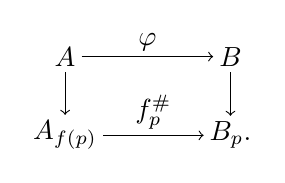
\begin{tikzpicture}[x=2.1cm,y=1.0cm,every node/.style={inner sep=2pt}]
\node (a) at (0,0) {$A$};
\node (b) at (1,0) {$B$};
\node (ap) at (0,-1) {$A_{f(\mathfrak p)}$};
\node (bp) at (1,-1) {$B_{\mathfrak p}$.};
\draw[->] (a) -- node[above] {$\varphi$} (b);
\draw[->] (a) -- (ap);
\draw[->] (b) -- (bp);
\draw[->] (ap) -- node[above] {$f^\#_{\mathfrak p}$} (bp);
\end{tikzpicture}
\]
}
% Contents from body/page-088.tex.
\ChapterSheet{88}{74}{\Goto{p-74}{II\quad Schemes}}{%
Since $f^\#$ is a local homomorphism, it follows that $\varphi^{-1}(\mathfrak p)=f(\mathfrak p)$, which shows that $f$ coincides with the map $\operatorname{Spec}B\to\operatorname{Spec}A$ induced by $\varphi$. Now it is immediate that $f^\#$ also is induced by $\varphi$, so that the morphism $(f,f^\#)$ of locally ringed spaces does indeed come from the homomorphism of rings $\varphi$.

\medskip
\noindent\hypertarget{result-II-2.3.0}{}\textbf{Caution 2.3.0.} Statement \Goto{result-II-2.3c}{(c)} of the proposition would be false, if in the definition of a morphism of locally ringed spaces, we did not insist that the induced maps on the stalks be \emph{local} homomorphisms of local rings (see \Goto{result-II-2.3.2}{(2.3.2)} below).

\medskip
Now we come to the definition of a scheme.

\medskip
\noindent\textbf{Definition.} An \emph{affine scheme} is a locally ringed space $(X,\mathcal O_X)$ which is isomorphic (as a locally ringed space) to the spectrum of some ring. A \emph{scheme} is a locally ringed space $(X,\mathcal O_X)$ in which every point has an open neighborhood $U$ such that the topological space $U$, together with the restricted sheaf $\mathcal O_X|_U$, is an affine scheme. We call $X$ the \emph{underlying topological space} of the scheme $(X,\mathcal O_X)$, and $\mathcal O_X$ its \emph{structure sheaf}. By abuse of notation we will often write simply $X$ for the scheme $(X,\mathcal O_X)$. If we wish to refer to the underlying topological space without its scheme structure, we write $\operatorname{sp}(X)$, read \textquotedblleft{}space of $X$.\textquotedblright{} A \emph{morphism} of schemes is a morphism as locally ringed spaces. An \emph{isomorphism} is a morphism with a two-sided inverse.

\medskip
\noindent\hypertarget{result-II-2.3.1}{}\textbf{Example 2.3.1.} If $k$ is a field, $\operatorname{Spec}k$ is an affine scheme whose topological space consists of one point, and whose structure sheaf consists of the field $k$.

\medskip
\noindent\hypertarget{result-II-2.3.2}{}\textbf{Example 2.3.2.} If $R$ is a discrete valuation ring, then $T=\operatorname{Spec}R$ is an affine scheme whose topological space consists of two points. One point $t_0$ is closed, with local ring $R$; the other point $t_1$ is open and dense, with local ring equal to $K$, the quotient field of $R$. The inclusion map $R\to K$ corresponds to the morphism $\operatorname{Spec}K\to T$ which sends the unique point of $\operatorname{Spec}K$ to $t_1$. There is another morphism of ringed spaces $\operatorname{Spec}K\to T$ which sends the unique point of $\operatorname{Spec}K$ to $t_0$, and uses the inclusion $R\to K$ to define the associated map $f^\#$ on structure sheaves. This morphism is \emph{not} induced by any homomorphism $R\to K$ as in (\Goto{result-II-2.3b}{2.3b},\Goto{result-II-2.3c}{c}), since it is not a morphism of \emph{locally ringed spaces}.

\medskip
\noindent\hypertarget{result-II-2.3.3}{}\textbf{Example 2.3.3.} If $k$ is a field, we define the \emph{affine line} over $k$, $\AffSpace[k]{1}$, to be $\operatorname{Spec}k[x]$. It has a point $\xi$, corresponding to the zero ideal, whose closure is the whole space. This is called a \emph{generic point}. The other points, which correspond to the maximal ideals in $k[x]$, are all closed points. They are
}
% Contents from body/page-089.tex.
\ChapterSheet{89}{75}{\Goto{sec-II-2}{2\quad Schemes}}{%
in one-to-one correspondence with the nonconstant monic irreducible polynomials in $x$. In particular, if $k$ is algebraically closed, the closed points of $\AffSpace[k]{1}$ are in one-to-one correspondence with elements of $k$.

\medskip
\noindent\hypertarget{result-II-2.3.4}{}\textbf{Example 2.3.4.} Let $k$ be an algebraically closed field, and consider the \emph{affine plane} over $k$, defined as $\AffSpace[k]{2}=\operatorname{Spec}k[x,y]$ (Fig.~\Goto{fig-book-6}{6}). The closed points of $\AffSpace[k]{2}$ are in one-to-one correspondence with ordered pairs of elements of $k$. Furthermore, the set of all closed points of $\AffSpace[k]{2}$, with the induced topology, is homeomorphic to the \emph{variety} called $\AffSpace{2}$ in Chapter \Goto{p-15}{I}. In addition to the closed points, there is a \emph{generic point} $\xi$, corresponding to the zero ideal of $k[x,y]$, whose closure is the whole space. Also, for each irreducible polynomial $f(x,y)$, there is a point $\eta$ whose closure consists of $\eta$ together with all closed points $(a,b)$ for which $f(a,b)=0$. We say that $\eta$ is a \emph{generic point} of the curve $f(x,y)=0$.

\smallskip
{\centering
\noindent\hypertarget{fig-book-6}{}\par\nobreak
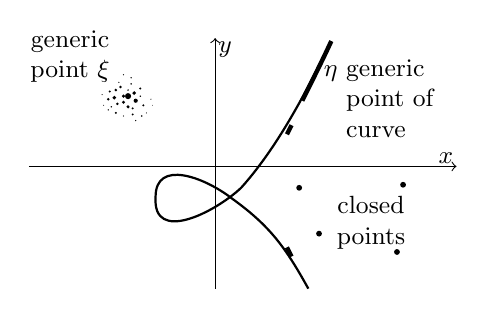
\begin{tikzpicture}[x=.55bp,y=-.55bp, every node/.style={inner sep=1pt,font=\small}]
\draw[->,thin] (0,86) -- (280,86) node[above left] {$x$};
\draw[->,thin] (122,166) -- (122,2) node[below right] {$y$};
\draw[line width=.8pt] (183,166) .. controls (168,139) and (158,125) .. (133,107)
  .. controls (115,93) and (83,81) .. (83,106)
  .. controls (81,137) and (122,116) .. (139,100)
  .. controls (165,71) and (184,32) .. (198,4);
\draw[line width=1.6pt] (179,43) .. controls (184,33) and (193,15) .. (198,4);
\draw[line width=1.6pt] (169,65) -- (172,59) (169,139) -- (172,145);
\foreach \x/\y in {177/100,190/130,241/142,245/98} \fill (\x,\y) circle[radius=1.05bp];
\foreach \x/\y/\r in {65/36/.3,60/34/.5,62/40/.6,57/36/.5,62/44/.6,67/32/.3,69/38/.7,58/45/.5,65/47/.6,65/40/1.1,70/43/.75,68/48/.4,56/41/.7,68/52/.4,52/42/.5,53/37/.4,54/47/.3,57/51/.4,62/53/.25,73/35/.4,73/40/.3,75/46/.4,59/31/.25,52/49/.25,74/53/.3,67/28/.25,70/56/.25,49/46/.17,48/39/.2,62/26/.2,80/42/.2,77/51/.2,81/46/.15}
  \fill (\x,\y) circle[radius=\r bp];
\node[align=center] at (27,14) {generic\\point $\xi$};
\node[align=left,anchor=west] at (191,43) {$\eta$ generic\\\phantom{$\eta$ }point of\\\phantom{$\eta$ }curve};
\node[align=center] at (224,123) {closed\\points};
\end{tikzpicture}\par\nobreak\smallskip
Figure 6.\enspace $\operatorname{Spec}k[x,y]$.\par}

\medskip
\noindent\hypertarget{result-II-2.3.5}{}\textbf{Example 2.3.5.} Let $X_1$ and $X_2$ be schemes, let $U_1\subseteq X_1$ and $U_2\subseteq X_2$ be open subsets, and let $\varphi\colon(U_1,\mathcal O_{X_1}|_{U_1})\to(U_2,\mathcal O_{X_2}|_{U_2})$ be an isomorphism of locally ringed spaces. Then we can define a scheme $X$, obtained by \emph{glueing} $X_1$ and $X_2$ along $U_1$ and $U_2$ via the isomorphism $\varphi$. The topological space of $X$ is the quotient of the disjoint union $X_1\cup X_2$ by the equivalence relation $x_1\sim\varphi(x_1)$ for each $x_1\in U_1$, with the quotient topology. Thus there are maps $i_1\colon X_1\to X$ and $i_2\colon X_2\to X$, and a subset $V\subseteq X$ is open if and only if $i_1^{-1}(V)$ is open in $X_1$ and $i_2^{-1}(V)$ is open in $X_2$. The structure sheaf $\mathcal O_X$ is defined as follows: for any open set $V\subseteq X$,
\[
\begin{split}
\mathcal O_X(V)=\{\langle s_1,s_2\rangle\mid &s_1\in\mathcal O_{X_1}(i_1^{-1}(V))\text{ and } s_2\in\mathcal O_{X_2}(i_2^{-1}(V))\text{ and}\\
&\varphi(s_1|_{i_1^{-1}(V)\cap U_1})=s_2|_{i_2^{-1}(V)\cap U_2}\}.
\end{split}
\]
Now it is clear that $\mathcal O_X$ is a sheaf, and that $(X,\mathcal O_X)$ is a locally ringed space. Furthermore, since $X_1$ and $X_2$ are schemes, it is clear that every point of $X$ has a neighborhood which is affine, hence $X$ is a scheme.

\medskip
\noindent\hypertarget{result-II-2.3.6}{}\textbf{Example 2.3.6.} As an example of glueing, let $k$ be a field, let $X_1=X_2=\AffSpace[k]{1}$, let $U_1=U_2=\AffSpace[k]{1}-\{P\}$, where $P$ is the point corresponding to the
}
% Contents from body/page-090.tex.
\ChapterSheet{90}{76}{\Goto{p-74}{II\quad Schemes}}{%
maximal ideal $(x)$, and let $\varphi\colon U_1\to U_2$ be the identity map. Let $X$ be obtained by glueing $X_1$ and $X_2$ along $U_1$ and $U_2$ via $\varphi$. We get an \textquotedblleft{}affine line with the point $P$ doubled.\textquotedblright{}

\[
\begin{tikzpicture}[x=1bp,y=1bp,baseline=-2bp]
\draw[thin] (-52,0) -- (-2,0) (2,0) -- (52,0);
\fill (0,1.8) circle[radius=.6bp] (0,-1.8) circle[radius=.6bp];
\end{tikzpicture}
\]
This is an example of a scheme which is not an affine scheme (!). It is also an example of a nonseparated scheme, as we will see later \Goto{result-II-4.0.1}{(4.0.1)}.

\medskip
Next we will define an important class of schemes, constructed from graded rings, which are analogous to projective varieties.

Let $S$ be a graded ring. See (I, \Goto{sec-I-2}{\S2}) for our conventions about graded rings. We denote by $S_+$ the ideal $\bigoplus_{d>0}S_d$.

We define the \emph{set} $\operatorname{Proj}S$ to be the set of all homogeneous prime ideals $\mathfrak p$, which do not contain all of $S_+$. If $\mathfrak a$ is a homogeneous ideal of $S$, we define the subset $V(\mathfrak a)=\{\mathfrak p\in\operatorname{Proj}S\mid\mathfrak p\supseteq\mathfrak a\}$.

\medskip
\noindent\hypertarget{result-II-2.4}{}\textbf{Lemma 2.4.}
\par{\leftskip=12pt\itshape
\hypertarget{result-II-2.4a}{}(a) If $\mathfrak a$ and $\mathfrak b$ are homogeneous ideals in $S$, then $V(\mathfrak a\mathfrak b)=V(\mathfrak a)\cup V(\mathfrak b)$.

\hypertarget{result-II-2.4b}{}(b) If $\{\mathfrak a_i\}$ is any family of homogeneous ideals of $S$, then $V(\sum\mathfrak a_i)=\bigcap V(\mathfrak a_i)$.\par}

\smallskip
\noindent\textsc{Proof.} The proofs are the same as for (\Goto{result-II-2.1a}{2.1a},\Goto{result-II-2.1b}{b}), taking into account the fact that a \EditionText{proper homogeneous ideal} $\mathfrak p$ is prime if and only if for any two \emph{homogeneous} elements $a,b\in S$, $ab\in\mathfrak p$ implies $a\in\mathfrak p$ or $b\in\mathfrak p$.

\medskip
Because of the lemma we can define a topology on $\operatorname{Proj}S$ by taking the closed subsets to be the subsets of the form $V(\mathfrak a)$.

Next we will define a sheaf of rings $\mathcal O$ on $\operatorname{Proj}S$. For each $\mathfrak p\in\operatorname{Proj}S$, we consider the ring $S_{(\mathfrak p)}$ of elements of degree zero in the localized ring $T^{-1}S$, where $T$ is the multiplicative system consisting of all \emph{homogeneous} elements of $S$ which are not in $\mathfrak p$. For any open subset $U\subseteq\operatorname{Proj}S$, we define $\mathcal O(U)$ to be the set of functions $s\colon U\to\coprod S_{(\mathfrak p)}$ such that for each $\mathfrak p\in U$, $s(\mathfrak p)\in S_{(\mathfrak p)}$, and such that $s$ is locally a quotient of elements of $S$: for each $\mathfrak p\in U$, there exists a neighborhood $V$ of $\mathfrak p$ in $U$, and homogeneous elements $a,f$ in $S$, of the same degree, such that for all $\mathfrak q\in V$, $f\notin\mathfrak q$, and $s(\mathfrak q)=a/f$ in $S_{(\mathfrak q)}$. Now it is clear that $\mathcal O$ is a presheaf of rings, with the natural restrictions, and it is also clear from the local nature of the definition that $\mathcal O$ is a sheaf.

\medskip
\noindent\textbf{Definition.} If $S$ is any graded ring, we define $(\operatorname{Proj}S,\mathcal O)$ to be the topological space together with the sheaf of rings constructed above.

\medskip
\noindent\hypertarget{result-II-2.5}{}\textbf{Proposition 2.5.} \emph{Let $S$ be a graded ring.}
\par{\leftskip=12pt\itshape
\hypertarget{result-II-2.5a}{}(a) For any $\mathfrak p\in\operatorname{Proj}S$, the stalk $\mathcal O_{\mathfrak p}$ is isomorphic to the local ring $S_{(\mathfrak p)}$.

\hypertarget{result-II-2.5b}{}(b) For any homogeneous $f\in S_+$, let $D_+(f)=\{\mathfrak p\in\operatorname{Proj}S\mid f\notin\mathfrak p\}$.\par}
}
% Contents from body/page-091.tex.
\ChapterSheet{91}{77}{\Goto{sec-II-2}{2\quad Schemes}}{%
{\leftskip=12pt\itshape
\noindent Then $D_+(f)$ is open in $\operatorname{Proj}S$. Furthermore, these open sets cover $\operatorname{Proj}S$, and for each such open set, we have an isomorphism of locally ringed spaces
\[
(D_+(f),\mathcal O|_{D_+(f)})\cong\operatorname{Spec}S_{(f)},
\]
where $S_{(f)}$ is the subring of elements of degree $0$ in the localized ring $S_f$.

\hypertarget{result-II-2.5c}{}(c) $\operatorname{Proj}S$ is a scheme.\par}

\medskip
\noindent\textsc{Proof.} Note first that \Goto{result-II-2.5a}{(a)} says that $\operatorname{Proj}S$ is a locally ringed space, and \Goto{result-II-2.5b}{(b)} tells us it is covered by open affine schemes, so \Goto{result-II-2.5c}{(c)} is a consequence of \Goto{result-II-2.5a}{(a)} and \Goto{result-II-2.5b}{(b)}.

The proof of \Goto{result-II-2.5a}{(a)} is practically identical to the proof of \Goto{result-II-2.2a}{(2.2a)} above, so is left to the reader.

To prove \Goto{result-II-2.5b}{(b)}, first note that $D_+(f)=\operatorname{Proj}S-V((f))$, so it is open. Since the elements of $\operatorname{Proj}S$ are those homogeneous prime ideals $\mathfrak p$ of $S$ which do not contain all of $S_+$, it follows that the open sets $D_+(f)$ for homogeneous $f\in S_+$ cover $\operatorname{Proj}S$. Now fix a homogeneous $f\in S_+$. We will define an isomorphism $(\varphi,\varphi^\#)$ of locally ringed spaces from $D_+(f)$ to $\operatorname{Spec}S_{(f)}$. There is a natural homomorphism of rings $S\to S_f$, and $S_{(f)}$ is a subring of $S_f$. For any homogeneous ideal $\mathfrak a\subseteq S$, let $\varphi(\mathfrak a)=(\mathfrak aS_f)\cap S_{(f)}$. In particular, if $\mathfrak p\in D_+(f)$, then $\varphi(\mathfrak p)\in\operatorname{Spec}S_{(f)}$, so this gives the map $\varphi$ as sets. The properties of localization show that $\varphi$ is bijective as a map from $D_+(f)$ to $\operatorname{Spec}S_{(f)}$. Furthermore, if $\mathfrak a$ is a homogeneous ideal of $S$, then $\mathfrak p\supseteq\mathfrak a$ if and only if $\varphi(\mathfrak p)\supseteq\varphi(\mathfrak a)$. Hence $\varphi$ is a homeomorphism. Note also if $\mathfrak p\in D_+(f)$, then the local rings $S_{(\mathfrak p)}$ and $(S_{(f)})_{\varphi(\mathfrak p)}$ are naturally isomorphic. These isomorphisms and the homeomorphism $\varphi$ induce a natural map of sheaves $\varphi^\#\colon\mathcal O_{\operatorname{Spec}S_{(f)}}\to\varphi_*(\mathcal O_{\operatorname{Proj}S}|_{D_+(f)})$ which one recognizes immediately to be an isomorphism. Hence $(\varphi,\varphi^\#)$ is an isomorphism of locally ringed spaces, as required.

\medskip
\noindent\hypertarget{result-II-2.5.1}{}\textbf{Example 2.5.1.} If $A$ is a ring, we define \emph{projective $n$-space} over $A$ to be the scheme $\Proj_A^n=\operatorname{Proj}A[x_0,\ldots,x_n]$. In particular, if $A$ is an algebraically closed field $k$, then $\Proj_k^n$ is a scheme whose subspace of closed points is naturally homeomorphic to the \emph{variety} called projective $n$-space---see (Ex.~\Goto{ex-II-2.14d}{2.14d}) below.

\medskip
Next we will show that the notion of scheme does in fact generalize the notion of variety. It is not quite true that a variety is a scheme. As we have already seen in the examples above, the underlying topological space of a scheme such as $\AffSpace[k]{1}$ or $\AffSpace[k]{2}$ has more points than the corresponding variety. However, we will show that there is a natural way of adding generic points (Ex.~\Goto{ex-II-2.9}{2.9}) for every \EditionText{irreducible closed subset} of a variety so that the variety becomes a scheme.

To state our result, we need a definition.
}
% Contents from body/page-092.tex.
\ChapterSheet{92}{78}{\Goto{p-74}{II\quad Schemes}}{%
\noindent\textbf{Definition.} Let $S$ be a fixed scheme. A \emph{scheme over $S$} is a scheme $X$, together with a morphism $X\to S$. If $X$ and $Y$ are schemes over $S$, a \emph{morphism of $X$ to $Y$ as schemes over $S$}, (also called an \emph{$S$-morphism}) is a morphism $f\colon X\to Y$ which is compatible with the given morphisms to $S$. We denote by $\mathfrak{Sch}(S)$ the category of schemes over $S$. If $A$ is a ring, then by abuse of notation we write $\mathfrak{Sch}(A)$ for the category of schemes over $\operatorname{Spec}A$.

\medskip
\noindent\hypertarget{result-II-2.6}{}\textbf{Proposition 2.6.} \emph{Let $k$ be an algebraically closed field. There is a natural fully faithful functor $t\colon\mathfrak{Var}(k)\to\mathfrak{Sch}(k)$ from the category of varieties over $k$ to schemes over $k$. For any variety $V$, its topological space is homeomorphic to the set of closed points of $\operatorname{sp}(t(V))$, and its sheaf of regular functions is obtained by restricting the structure sheaf of $t(V)$ via this homeomorphism.}

\smallskip
\noindent\textsc{Proof.} To begin with, let $X$ be any topological space, and let $t(X)$ be the set of (nonempty) irreducible closed subsets of $X$. If $Y$ is a closed subset of $X$, then $t(Y)\subseteq t(X)$. Furthermore, $t(Y_1\cup Y_2)=t(Y_1)\cup t(Y_2)$ and $t(\bigcap Y_i)=\bigcap t(Y_i)$. So we can define a topology on $t(X)$ by taking as closed sets the subsets of the form $t(Y)$, where $Y$ is a closed subset of $X$. If $f\colon X_1\to X_2$ is a continuous map, then we obtain a map $t(f)\colon t(X_1)\to t(X_2)$ by sending an irreducible closed subset to the closure of its image. Thus $t$ is a functor on topological spaces. Furthermore, one can define a continuous map $\alpha\colon X\to t(X)$ by $\alpha(P)=\{P\}^{-}$. Note that $\alpha$ induces a \emph{bijection} between the set of open subsets of $X$ and the set of open subsets of $t(X)$.

Now let $k$ be an algebraically closed field. Let $V$ be a variety over $k$, and let $\mathcal O_V$ be its sheaf of regular functions \Goto{result-II-1.0.1}{(1.0.1)}. We will show that $(t(V),\alpha_*(\mathcal O_V))$ is a scheme over $k$. Since any variety can be covered by open affine subvarieties (I, \Goto{result-I-4.3}{4.3}), it will be sufficient to show that if $V$ is affine, then $(t(V),\alpha_*(\mathcal O_V))$ is a scheme. So let $V$ be an affine variety with affine coordinate ring $A$. We define a morphism of locally ringed spaces
\[
\beta\colon(V,\mathcal O_V)\to X=\operatorname{Spec}A
\]
as follows. For each point $P\in V$, let $\beta(P)=\mathfrak m_P$, the ideal of $A$ consisting of all regular functions which vanish at $P$. Then by (I, \Goto{result-I-3.2}{3.2b}), $\beta$ is a bijection of $V$ onto the set of closed points of $X$. It is easy to see that $\beta$ is a homeomorphism onto its image. Now for any open set $U\subseteq X$, we will define a homomorphism of rings $\mathcal O_X(U)\to\beta_*(\mathcal O_V)(U)=\mathcal O_V(\beta^{-1}U)$. Given a section $s\in\mathcal O_X(U)$, and given a point $P\in\beta^{-1}(U)$, we define $s(P)$ by taking the image of $s$ in the stalk $\mathcal O_{X,\beta(P)}$, which is isomorphic to the local ring $A_{\mathfrak m_P}$, and then passing to the quotient ring $A_{\mathfrak m_P}/\mathfrak m_P$ which is isomorphic to the field $k$. Thus $s$ gives a function from $\beta^{-1}(U)$ to $k$. It is easy to see that this is a regular function, and that this map gives an isomorphism $\mathcal O_X(U)\cong\mathcal O_V(\beta^{-1}U)$. Finally, since the prime ideals of $A$ are in $1$-$1$ correspondence with the irreducible closed subsets of $V$ (see (I, \Goto{result-I-1.4}{1.4}) and proof), these remarks show that $(X,\mathcal O_X)$ is isomorphic to $(t(V),\alpha_*\mathcal O_V)$, so the latter is indeed an affine scheme.
}
% Contents from body/page-093.tex.
\ChapterSheet{93}{79}{\Goto{sec-II-2}{2\quad Schemes}}{%
\indent To give a morphism of $(t(V),\alpha_*\mathcal O_V)$ to $\operatorname{Spec}k$, we have only to give a homomorphism of rings $k\to\Gamma(t(V),\alpha_*\mathcal O_V)=\Gamma(V,\mathcal O_V)$. We send $\lambda\in k$ to the constant function $\lambda$ on $V$. Thus $t(V)$ becomes a scheme over $k$. Finally, if $V$ and $W$ are two varieties, then one can check (Ex.~\Goto{ex-II-2.15}{2.15}) that the natural map
\[
\operatorname{Hom}_{\mathfrak{Var}(k)}(V,W)\to\operatorname{Hom}_{\mathfrak{Sch}(k)}(t(V),t(W))
\]
is bijective. This shows that the functor $t\colon\mathfrak{Var}(k)\to\mathfrak{Sch}(k)$ is fully faithful. In particular it implies that $t(V)$ is isomorphic to $t(W)$ if and only if $V$ is isomorphic to $W$.

It is clear from the construction that $\alpha\colon V\to t(V)$ induces a homeomorphism from $V$ onto the set of closed points of $t(V)$, with the induced topology.

\medskip
\emph{Note.} We will see later \Goto{result-II-4.10}{(4.10)} what the image of the functor $t$ is.

\bigskip
\noindent\textsc{Exercises}\par\nobreak\smallskip
{\fontsize{9.2}{10.65}\selectfont\leftskip=22pt\relax
\noindent\hypertarget{ex-II-2.1}{}\llap{\textbf{2.1.}\enspace}Let $A$ be a ring, let $X=\operatorname{Spec}A$, let $f\in A$ and let $D(f)\subseteq X$ be the open complement of $V((f))$. Show that the locally ringed space $(D(f),\mathcal O_X|_{D(f)})$ is isomorphic to $\operatorname{Spec}A_f$.

\smallskip
\noindent\hypertarget{ex-II-2.2}{}\llap{\textbf{2.2.}\enspace}Let $(X,\mathcal O_X)$ be a scheme, and let $U\subseteq X$ be any open subset. Show that $(U,\mathcal O_X|_U)$ is a scheme. We call this the \emph{induced scheme structure} on the open set $U$, and we refer to $(U,\mathcal O_X|_U)$ as an \emph{open subscheme} of $X$.

\smallskip
\noindent\hypertarget{ex-II-2.3}{}\llap{\textbf{2.3.}\enspace}\emph{Reduced Schemes.} A scheme $(X,\mathcal O_X)$ is \emph{reduced} if for every open set $U\subseteq X$, the ring $\mathcal O_X(U)$ has no nilpotent elements.

{\advance\leftskip by 12pt
\noindent\hypertarget{ex-II-2.3a}{}\llap{(a)\enspace}Show that $(X,\mathcal O_X)$ is reduced if and only if for every $P\in X$, the local ring $\mathcal O_{X,P}$ has no nilpotent elements.

\noindent\hypertarget{ex-II-2.3b}{}\llap{(b)\enspace}Let $(X,\mathcal O_X)$ be a scheme. Let $(\mathcal O_X)_{\mathrm{red}}$ be the sheaf associated to the presheaf $U\mapsto\mathcal O_X(U)_{\mathrm{red}}$, where for any ring $A$, we denote by $A_{\mathrm{red}}$ the quotient of $A$ by its ideal of nilpotent elements. Show that $(X,(\mathcal O_X)_{\mathrm{red}})$ is a scheme. We call it the \emph{reduced scheme} associated to $X$, and denote it by $X_{\mathrm{red}}$. Show that there is a morphism of schemes $X_{\mathrm{red}}\to X$, which is a homeomorphism on the underlying topological spaces.

\noindent\hypertarget{ex-II-2.3c}{}\llap{(c)\enspace}Let $f\colon X\to Y$ be a morphism of schemes, and assume that $X$ is reduced. Show that there is a unique morphism $g\colon X\to Y_{\mathrm{red}}$ such that $f$ is obtained by composing $g$ with the natural map $Y_{\mathrm{red}}\to Y$.\par}

\smallskip
\noindent\hypertarget{ex-II-2.4}{}\llap{\textbf{2.4.}\enspace}Let $A$ be a ring and let $(X,\mathcal O_X)$ be a scheme. Given a morphism $f\colon X\to\operatorname{Spec}A$, we have an associated map on sheaves $f^\#\colon\mathcal O_{\operatorname{Spec}A}\to f_*\mathcal O_X$. Taking global sections we obtain a homomorphism $A\to\Gamma(X,\mathcal O_X)$. Thus there is a natural map
\[
\alpha\colon\operatorname{Hom}_{\mathfrak{Sch}}(X,\operatorname{Spec}A)\to\operatorname{Hom}_{\mathfrak{Rings}}(A,\Gamma(X,\mathcal O_X)).
\]
Show that $\alpha$ is bijective (cf. (I, \Goto{result-I-3.5}{3.5}) for an analogous statement about varieties).

\smallskip
\noindent\hypertarget{ex-II-2.5}{}\llap{\textbf{2.5.}\enspace}Describe $\operatorname{Spec}\mathbf Z$, and show that it is a final object for the category of schemes, i.e., each scheme $X$ admits a unique morphism to $\operatorname{Spec}\mathbf Z$.\par}
}
% Contents from body/page-094.tex.
\ChapterSheet{94}{80}{\Goto{p-74}{II\quad Schemes}}{%
{\fontsize{9.2}{9.97}\selectfont\parskip=.2pt\leftskip=21pt\relax
\noindent\hypertarget{ex-II-2.6}{}\llap{\textbf{2.6.}\enspace}Describe the spectrum of the zero ring, and show that it is an initial object for the category of schemes. (According to our conventions, all ring homomorphisms must take $1$ to $1$. Since $0=1$ in the zero ring, we see that each ring $R$ admits a unique homomorphism to the zero ring, but that there is no homomorphism from the zero ring to $R$ unless $0=1$ in $R$.)

\vspace{2pt}
\noindent\hypertarget{ex-II-2.7}{}\llap{\textbf{2.7.}\enspace}Let $X$ be a scheme. For any $x\in X$, let $\mathcal O_x$ be the local ring at $x$, and $\mathfrak m_x$ its maximal ideal. We define the \emph{residue field} of $x$ on $X$ to be the field $k(x)=\mathcal O_x/\mathfrak m_x$. Now let $K$ be any field. Show that to give a morphism of $\operatorname{Spec}K$ to $X$ it is equivalent to give a point $x\in X$ and an inclusion map $k(x)\to K$.

\vspace{2pt}
\noindent\hypertarget{ex-II-2.8}{}\llap{\textbf{2.8.}\enspace}Let $X$ be a scheme. For any point $x\in X$, we define the \emph{Zariski tangent space} $T_x$ to $X$ at $x$ to be the dual of the $k(x)$-vector space $\mathfrak m_x/\mathfrak m_x^2$. Now assume that $X$ is a scheme over a field $k$, and let $k[\varepsilon]/\varepsilon^2$ be the \emph{ring of dual numbers} over $k$. Show that to give a $k$-morphism of $\operatorname{Spec}k[\varepsilon]/\varepsilon^2$ to $X$ is equivalent to giving a point $x\in X$, \emph{rational over $k$} (i.e., such that $k(x)=k$), and an element of $T_x$.

\vspace{2pt}
\noindent\hypertarget{ex-II-2.9}{}\llap{\textbf{2.9.}\enspace}If $X$ is a topological space, and $Z$ an irreducible closed subset of $X$, a \emph{generic point} for $Z$ is a point $\zeta$ such that $Z=\{\zeta\}^{-}$. If $X$ is a scheme, show that every (nonempty) irreducible closed subset has a unique generic point.

\vspace{2pt}
\noindent\hypertarget{ex-II-2.10}{}\llap{\textbf{2.10.}\enspace}Describe $\operatorname{Spec}\mathbf R[x]$. How does its topological space compare to the set $\mathbf R$? To $\mathbf C$?

\vspace{2pt}
\noindent\hypertarget{ex-II-2.11}{}\llap{\textbf{2.11.}\enspace}Let $k=\mathbf F_p$ be the finite field with $p$ elements. Describe $\operatorname{Spec}k[x]$. What are the residue fields of its points? How many points are there with a given residue field?

\vspace{2pt}
\noindent\hypertarget{ex-II-2.12}{}\llap{\textbf{2.12.}\enspace}\emph{Glueing Lemma.} Generalize the glueing procedure described in the text \Goto{result-II-2.3.5}{(2.3.5)} as follows. Let $\{X_i\}$ be a family of schemes (possible infinite). For each $i\ne j$, suppose given an open subset $U_{ij}\subseteq X_i$, and let it have the induced scheme structure (Ex.~\Goto{ex-II-2.2}{2.2}). Suppose also given for each $i\ne j$ an isomorphism of schemes $\varphi_{ij}\colon U_{ij}\to U_{ji}$ \EditionText{and put $U_{ii}=X_i$ and $\varphi_{ii}=\operatorname{id}_{X_i}$. Assume that} (1) for each $i,j$, $\varphi_{ji}=\varphi_{ij}^{-1}$, and (2) for each $i,j,k$, $\varphi_{ij}(U_{ij}\cap U_{ik})=U_{ji}\cap U_{jk}$, and $\varphi_{ik}=\varphi_{jk}\circ\varphi_{ij}$ on $U_{ij}\cap U_{ik}$. Then show that there is a scheme $X$, together with morphisms $\psi_i\colon X_i\to X$ for each $i$, such that (1) $\psi_i$ is an isomorphism of $X_i$ onto an open subscheme of $X$, (2) the $\psi_i(X_i)$ cover $X$, (3) $\psi_i(U_{ij})=\psi_i(X_i)\cap\psi_j(X_j)$ and (4) $\psi_i=\psi_j\circ\varphi_{ij}$ on $U_{ij}$. We say that $X$ is obtained by \emph{glueing} the schemes $X_i$ along the isomorphisms $\varphi_{ij}$. An interesting special case is when the family $X_i$ is arbitrary, but the $U_{ij}$ and $\varphi_{ij}$ are all empty\EditionText{ for $i\ne j$}. Then the scheme $X$ is called the \emph{disjoint union} of the $X_i$, and is denoted $\coprod X_i$.

\vspace{2pt}
\noindent\hypertarget{ex-II-2.13}{}\llap{\textbf{2.13.}\enspace}A topological space is \emph{quasi-compact} if every open cover has a finite subcover.

{\advance\leftskip by 12pt
\noindent\hypertarget{ex-II-2.13a}{}\llap{(a)\enspace}Show that a topological space is noetherian (I, \Goto{sec-I-1}{\S1}) if and only if every open subset is quasi-compact.

\noindent\hypertarget{ex-II-2.13b}{}\llap{(b)\enspace}If $X$ is an affine scheme, show that $\operatorname{sp}(X)$ is quasi-compact, but not in general noetherian. We say a scheme $X$ is \emph{quasi-compact} if $\operatorname{sp}(X)$ is.

\noindent\hypertarget{ex-II-2.13c}{}\llap{(c)\enspace}If $A$ is a noetherian ring, show that $\operatorname{sp}(\operatorname{Spec}A)$ is a noetherian topological space.

\noindent\hypertarget{ex-II-2.13d}{}\llap{(d)\enspace}Give an example to show that $\operatorname{sp}(\operatorname{Spec}A)$ can be noetherian even when $A$ is not.\par}

\vspace{2pt}
{\advance\leftskip by 12pt
\noindent\hypertarget{ex-II-2.14}{}\llap{\textbf{2.14.}\hspace{13.5pt}\enspace}\hypertarget{ex-II-2.14a}{}\llap{(a)\enspace}Let $S$ be a graded ring. Show that $\operatorname{Proj}S=\varnothing$ if and only if every element of $S_+$ is nilpotent.

\noindent\hypertarget{ex-II-2.14b}{}\llap{(b)\enspace}Let $\varphi\colon S\to T$ be a graded homomorphism of graded rings (preserving degrees). Let $U=\{\mathfrak p\in\operatorname{Proj}T\mid\mathfrak p\nsupseteq\varphi(S_+)\}$. Show that $U$ is an open subset of $\operatorname{Proj}T$, and show that $\varphi$ determines a natural morphism $f\colon U\to\operatorname{Proj}S$.\par}\par}
}
% Contents from body/page-095.tex.
\ChapterSheet{95}{81}{\Goto{sec-II-2}{2\quad Schemes}}{%
{\fontsize{9.2}{10.65}\selectfont\leftskip=22pt\relax
{\advance\leftskip by 12pt
\noindent\hypertarget{ex-II-2.14c}{}\llap{(c)\enspace}The morphism $f$ can be an isomorphism even when $\varphi$ is not. For example, suppose that $\varphi_d\colon S_d\to T_d$ is an isomorphism for all $d\geq d_0$, where $d_0$ is an integer. Then show that $U=\operatorname{Proj}T$ and the morphism $f\colon\operatorname{Proj}T\to\operatorname{Proj}S$ is an isomorphism.

\noindent\hypertarget{ex-II-2.14d}{}\llap{(d)\enspace}Let $V$ be a projective variety with homogeneous coordinate ring $S$ (I, \Goto{sec-I-2}{\S2}). Show that $t(V)\cong\operatorname{Proj}S$.\par}

\smallskip
{\advance\leftskip by 12pt
\noindent\hypertarget{ex-II-2.15}{}\llap{\textbf{2.15.}\hspace{13.5pt}\enspace}\hypertarget{ex-II-2.15a}{}\llap{(a)\enspace}Let $V$ be a variety over the algebraically closed field $k$. Show that a point $P\in t(V)$ is a closed point if and only if its residue field is $k$.

\noindent\hypertarget{ex-II-2.15b}{}\llap{(b)\enspace}If $f\colon X\to Y$ is a morphism of schemes over $k$, and if $P\in X$ is a point with residue field $k$, then $f(P)\in Y$ also has residue field $k$.

\noindent\hypertarget{ex-II-2.15c}{}\llap{(c)\enspace}Now show that if $V,W$ are any two varieties over $k$, then the natural map
\[
\operatorname{Hom}_{\mathfrak{Var}}(V,W)\to\operatorname{Hom}_{\mathfrak{Sch}/k}(t(V),t(W))
\]
is bijective. (Injectivity is easy. The hard part is to show it is surjective.)\par}

\smallskip
\noindent\hypertarget{ex-II-2.16}{}\llap{\textbf{2.16.}\enspace}Let $X$ be a scheme, let $f\in\Gamma(X,\mathcal O_X)$, and define $X_f$ to be the subset of points $x\in X$ such that the stalk $f_x$ of $f$ at $x$ is not contained in the maximal ideal $\mathfrak m_x$ of the local ring $\mathcal O_x$.

{\advance\leftskip by 12pt
\noindent\hypertarget{ex-II-2.16a}{}\llap{(a)\enspace}If $U=\operatorname{Spec}B$ is an open \emph{affine} subscheme of $X$, and if $\bar f\in B=\Gamma(U,\mathcal O_X|_U)$ is the restriction of $f$, show that $U\cap X_f=D(\bar f)$. Conclude that $X_f$ is an open subset of $X$.

\noindent\hypertarget{ex-II-2.16b}{}\llap{(b)\enspace}Assume that $X$ is quasi-compact. Let $A=\Gamma(X,\mathcal O_X)$, and let $a\in A$ be an element whose restriction to $X_f$ is $0$. Show that for some $n>0$, $f^na=0$. [\emph{Hint:} Use an open affine cover of $X$.]

\noindent\hypertarget{ex-II-2.16c}{}\llap{(c)\enspace}Now assume that $X$ has a finite cover by open affines $U_i$ such that each intersection $U_i\cap U_j$ is quasi-compact. (This hypothesis is satisfied, for example, if $\operatorname{sp}(X)$ is noetherian.) Let $b\in\Gamma(X_f,\mathcal O_{X_f})$. Show that for some $n>0$, $f^nb$ is the restriction of an element of $A$.

\noindent\hypertarget{ex-II-2.16d}{}\llap{(d)\enspace}With the hypothesis of \Goto{ex-II-2.16c}{(c)}, conclude that $\Gamma(X_f,\mathcal O_{X_f})\cong A_f$.\par}

\smallskip
\noindent\hypertarget{ex-II-2.17}{}\llap{\textbf{2.17.}\enspace}\emph{A Criterion for Affineness.}

{\advance\leftskip by 12pt
\noindent\hypertarget{ex-II-2.17a}{}\llap{(a)\enspace}Let $f\colon X\to Y$ be a morphism of schemes, and suppose that $Y$ can be covered by open subsets $U_i$, such that for each $i$, the induced map $f^{-1}(U_i)\to U_i$ is an isomorphism. Then $f$ is an isomorphism.

\noindent\hypertarget{ex-II-2.17b}{}\llap{(b)\enspace}A scheme $X$ is affine if and only if there is a finite set of elements $f_1,\ldots,f_r\in A=\Gamma(X,\mathcal O_X)$, such that the open subsets $X_{f_i}$ are affine, and $f_1,\ldots,f_r$ generate the unit ideal in $A$. [\emph{Hint:} Use (Ex.~\Goto{ex-II-2.4}{2.4}) and (Ex.~\Goto{ex-II-2.16d}{2.16d}) above.]\par}

\smallskip
\noindent\hypertarget{ex-II-2.18}{}\llap{\textbf{2.18.}\enspace}In this exercise, we compare some properties of a ring homomorphism to the induced morphism of the spectra of the rings.

{\advance\leftskip by 12pt
\noindent\hypertarget{ex-II-2.18a}{}\llap{(a)\enspace}Let $A$ be a ring, $X=\operatorname{Spec}A$, and $f\in A$. Show that $f$ is nilpotent if and only if $D(f)$ is empty.

\noindent\hypertarget{ex-II-2.18b}{}\llap{(b)\enspace}Let $\varphi\colon A\to B$ be a homomorphism of rings, and let $f\colon Y=\operatorname{Spec}B\to X=\operatorname{Spec}A$ be the induced morphism of affine schemes. Show that $\varphi$ is injective if and only if the map of sheaves $f^\#\colon\mathcal O_X\to f_*\mathcal O_Y$ is injective. Show furthermore in that case $f$ is \emph{dominant}, i.e., $f(Y)$ is dense in $X$.

\noindent\hypertarget{ex-II-2.18c}{}\llap{(c)\enspace}With the same notation, show that if $\varphi$ is surjective, then $f$ is a homeomorphism of $Y$ onto a closed subset of $X$, and $f^\#\colon\mathcal O_X\to f_*\mathcal O_Y$ is surjective.\par}\par}
}
% Contents from body/page-096.tex.
\BookMark{1}{2.3  First Properties of Schemes}{sec-II-3}
\ChapterSheet{96}{82}{\Goto{p-74}{II\quad Schemes}}{%
\noindent\hangindent=3em\hspace*{1.7em}(d) Prove the converse to (c), namely, if $f\colon Y\to X$ is a homeomorphism onto a closed subset, and $f^\#\colon\mathcal O_X\to f_*\mathcal O_Y$ is surjective, then $\varphi$ is surjective. [\emph{Hint:} Consider $X'=\operatorname{Spec}(A/\ker\varphi)$ and use (b) and (c).]

\smallskip
\noindent\hypertarget{ex-II-2.19}{}\textbf{2.19.} Let $A$ be a ring. Show that the following conditions are equivalent:
\begin{enumerate}[label=(\roman*),nosep,leftmargin=2.4em]
\item $\operatorname{Spec}A$ is disconnected;
\item there exist nonzero elements $e_1,e_2\in A$ such that $e_1e_2=0$, $e_1^2=e_1$, $e_2^2=e_2$, $e_1+e_2=1$ (these elements are called \emph{orthogonal idempotents});
\item $A$ is isomorphic to a direct product $A_1\times A_2$ of two nonzero rings.
\end{enumerate}

\medskip
\noindent\hypertarget{sec-II-3}{}{\large\bfseries 3\quad First Properties of Schemes}\par
\smallskip
In this section we will give some of the first properties of schemes. In particular we will discuss open and closed subschemes, and products of schemes. In the exercises we introduce the notion of constructible subsets, and study the dimension of the fibres of a morphism.

\smallskip
\noindent\textbf{Definition.} A scheme is \emph{connected} if its topological space is connected. A scheme is \emph{irreducible} if its topological space is irreducible.

\smallskip
\noindent\textbf{Definition.} A scheme $X$ is \emph{reduced} if for every open set $U$, the ring $\mathcal O_X(U)$ has no nilpotent elements. Equivalently (Ex. \Goto{ex-II-2.3}{2.3}), $X$ is reduced if and only if the local rings $\mathcal O_P$, for all $P\in X$, have no nilpotent elements.

\smallskip
\noindent\hypertarget{err-II-3-integral}{}\textbf{Definition.} A scheme $X$ is \emph{integral} if \EditionText{it is nonempty and for every nonempty open set $U\subseteq X$}, the ring $\mathcal O_X(U)$ is an integral domain.

\smallskip
\noindent\hypertarget{result-II-3.0.1}{}\textbf{Example 3.0.1.} If $X=\operatorname{Spec}A$ is an affine scheme, then $X$ is irreducible if and only if the nilradical $\operatorname{nil}A$ of $A$ is prime; $X$ is reduced if and only if $\operatorname{nil}A=0$; and $X$ is integral if and only if $A$ is an integral domain.

\smallskip
\noindent\hypertarget{result-II-3.1}{}\textbf{Proposition 3.1.} \emph{A scheme is integral if and only if it is both reduced and irreducible.}

\smallskip
\noindent\textsc{Proof.} Clearly an integral scheme is reduced. If $X$ is not irreducible, then one can find two nonempty disjoint open subsets $U_1$ and $U_2$. Then $\mathcal O(U_1\cup U_2)=\mathcal O(U_1)\times\mathcal O(U_2)$ which is not an integral domain. Thus integral implies irreducible.

Conversely, suppose that $X$ is reduced and irreducible. Let $U\subseteq X$ be an \EditionText{nonempty }open subset, and suppose that there are elements $f,g\in\mathcal O(U)$ with $fg=0$. Let $Y=\{x\in U\mid f_x\in\mathfrak m_x\}$, and let $Z=\{x\in U\mid g_x\in\mathfrak m_x\}$. Then $Y$ and $Z$ are closed subsets (Ex. \Goto{ex-II-2.16}{2.16a}), and $Y\cup Z=U$. But $X$ is irreducible, so $U$ is irreducible, so one of $Y$ or $Z$ is equal to $U$, say $Y=U$. But then the restriction of $f$ to any open affine subset of $U$ will be nilpotent (Ex. \Goto{ex-II-2.18}{2.18a}), hence zero, so $f$ is zero. This shows that $X$ is integral.}
% Contents from body/page-097.tex.
\ChapterSheet{97}{83}{\Goto{sec-II-3}{3\quad First Properties of Schemes}}{%
\noindent\textbf{Definition.} A scheme $X$ is \emph{locally noetherian} if it can be covered by open affine subsets $\operatorname{Spec}A_i$, where each $A_i$ is a noetherian ring. $X$ is \emph{noetherian} if it is locally noetherian and quasi-compact. Equivalently, $X$ is noetherian if it can be covered by a finite number of open affine subsets $\operatorname{Spec}A_i$, with each $A_i$ a noetherian ring.

\smallskip
\noindent\hypertarget{result-II-3.1.1}{}\textbf{Caution 3.1.1.} If $X$ is a noetherian scheme, then $\operatorname{sp}(X)$ is a noetherian topological space, but not conversely (Ex. \Goto{ex-II-2.13}{2.13}) and (Ex. \Goto{ex-II-3.17}{3.17}).

Note that in this definition we do not require that every open affine subset be the spectrum of a noetherian ring. So while it is obvious from the definition that the spectrum of a noetherian ring is a noetherian scheme, the converse is not obvious. It is a question of showing that the noetherian property is a \textquotedblleft{}local property\textquotedblright{}. We will often encounter similar situations later in defining properties of a scheme or of a morphism of schemes, so we will give a careful statement and proof of the local nature of the noetherian property, to illustrate this type of situation.

\medskip
\noindent\hypertarget{result-II-3.2}{}\textbf{Proposition 3.2.} \emph{A scheme $X$ is locally noetherian if and only if for every open affine subset $U=\operatorname{Spec}A$, $A$ is a noetherian ring. In particular, an affine scheme $X=\operatorname{Spec}A$ is a noetherian scheme if and only if the ring $A$ is a noetherian ring.}

\smallskip
\noindent\textsc{Proof.} The \textquotedblleft{}if\textquotedblright{} part follows from the definition, so we have to show if $X$ is locally noetherian, and if $U=\operatorname{Spec}A$ is an open affine subset, then $A$ is a noetherian ring. First note that if $B$ is a noetherian ring, so is any localization $B_f$. The open subsets $D(f)\cong\operatorname{Spec}B_f$ form a base for the topology of $\operatorname{Spec}B$. Hence on a locally noetherian scheme $X$ there is a base for the topology consisting of the spectra of noetherian rings. In particular, our open set $U$ can be covered by spectra of noetherian rings.

So we have reduced to proving the following statement: let $X=\operatorname{Spec}A$ be an affine scheme, which can be covered by open subsets which are spectra of noetherian rings. Then $A$ is noetherian. Let $U=\operatorname{Spec}B$ be an open subset of $X$, with $B$ noetherian. Then for some $f\in A$, $D(f)\subseteq U$. Let $\bar f$ be the image of $f$ in $B$. Then $A_f\cong B_{\bar f}$, hence $A_f$ is noetherian. So we can cover $X$ by open subsets $D(f)\cong\operatorname{Spec}A_f$ with $A_f$ noetherian. Since $X$ is quasi-compact, a finite number will do.

So now we have reduced to a purely algebraic problem: $A$ is a ring, $f_1,\ldots,f_r$ are a finite number of elements of $A$, which generate the unit ideal, and each localization $A_{f_i}$ is noetherian. We have to show $A$ is noetherian. First we establish a lemma. Let $\mathfrak a\subseteq A$ be an ideal, and let $\varphi_i\colon A\to A_{f_i}$ be the localization map, $i=1,\ldots,r$. Then
\[
\mathfrak a=\bigcap\varphi_i^{-1}(\varphi_i(\mathfrak a)\cdot A_{f_i}).
\]
The inclusion $\subseteq$ is obvious. Conversely, given an element $b\in A$ contained}
% Contents from body/page-098.tex.
\ChapterSheet{98}{84}{\Goto{p-74}{II\quad Schemes}}{%
\noindent in this intersection, we can write $\varphi_i(b)=a_i/f_i^{n_i}$ in $A_{f_i}$ for each $i$, where $a_i\in\mathfrak a$, and $n_i>0$. Increasing the $n_i$ if necessary, we can make them all equal to a fixed $n$. This means that in $A$ we have
\[
f_i^{m_i}(f_i^nb-a_i)=0
\]
for some $m_i$. And as before, we can make all the $m_i=m$. Thus $f_i^{m+n}b\in\mathfrak a$ for each $i$. Since $f_1,\ldots,f_r$ generate the unit ideal, the same is true of their $N$th powers for any $N$. Take $N=n+m$. Then we have $1=\sum c_i f_i^N$ for suitable $c_i\in A$. Hence
\[
b=\sum c_i f_i^N b\in\mathfrak a
\]
as required.

Now we can easily show that $A$ is noetherian. Let $\mathfrak a_1\subseteq\mathfrak a_2\subseteq\cdots$ be an ascending chain of ideals in $A$. Then for each $i$,
\[
\varphi_i(\mathfrak a_1)\cdot A_{f_i}\subseteq\varphi_i(\mathfrak a_2)\cdot A_{f_i}\subseteq\cdots
\]
is an ascending chain of ideals in $A_{f_i}$, which must become stationary because $A_{f_i}$ is noetherian. There are only finitely many $A_{f_i}$, so from the lemma we conclude that the original chain is eventually stationary, and hence $A$ is noetherian.

\medskip
\noindent\textbf{Definition.} A morphism $f\colon X\to Y$ of schemes is \emph{locally of finite type} if there exists a covering of $Y$ by open affine subsets $V_i=\operatorname{Spec}B_i$, such that for each $i$, $f^{-1}(V_i)$ can be covered by open affine subsets $U_{ij}=\operatorname{Spec}A_{ij}$, where each $A_{ij}$ is a finitely generated $B_i$-algebra. The morphism $f$ is \emph{of finite type} if in addition each $f^{-1}(V_i)$ can be covered by a finite number of the $U_{ij}$.

\smallskip
\noindent\textbf{Definition.} A morphism $f\colon X\to Y$ is a \emph{finite} morphism if there exists a covering of $Y$ by open affine subsets $V_i=\operatorname{Spec}B_i$, such that for each $i$, $f^{-1}(V_i)$ is affine, equal to $\operatorname{Spec}A_i$, where $A_i$ is a $B_i$-algebra which is a finitely generated $B_i$-module.

Note in each of these definitions that a property of a morphism $f\colon X\to Y$ is defined by the existence of an open affine cover of $Y$ with certain properties. In fact in each case it is equivalent to require the given property for every open affine subset of $Y$ (Ex. \Goto{ex-II-3.1}{3.1}--\Goto{ex-II-3.4}{3.4}).

\medskip
\noindent\hypertarget{result-II-3.2.1}{}\textbf{Example 3.2.1.} If $V$ is a variety over an algebraically closed field $k$, then the associated scheme $t(V)$ (see \Goto{result-II-2.6}{(2.6)}) is an integral noetherian scheme of finite type over $k$. Indeed, $V$ can be covered by a finite number of open affine subvarieties \Goto{result-I-4.3}{(I, 4.3)}, so $t(V)$ can be covered by a finite number of open affines of the form $\operatorname{Spec}A_i$, where each $A_i$ is an integral domain which is a finitely generated $k$-algebra and hence noetherian.}
% Contents from body/page-099.tex.
\ChapterSheet{99}{85}{\Goto{sec-II-3}{3\quad First Properties of Schemes}}{%
\noindent\hypertarget{result-II-3.2.2}{}\textbf{Example 3.2.2.} If $P$ is a point of a variety $V$, with local ring $\mathcal O_P$, then $\operatorname{Spec}\mathcal O_P$ is an integral noetherian scheme, which is not in general of finite type over $k$.

Now we come to open and closed subschemes.

\smallskip
\noindent\textbf{Definition.} An \emph{open subscheme} of a scheme $X$ is a scheme $U$, whose topological space is an open subset of $X$, and whose structure sheaf $\mathcal O_U$ is isomorphic to the restriction $\mathcal O_X|_U$ of the structure sheaf of $X$. An \emph{open immersion} is a morphism $f\colon X\to Y$ which induces an isomorphism of $X$ with an open subscheme of $Y$.

Note that every open subset of a scheme carries a unique structure of open subscheme (Ex. \Goto{ex-II-2.2}{2.2}).

\smallskip
\noindent\textbf{Definition.} A \emph{closed immersion} is a morphism $f\colon Y\to X$ of schemes such that $f$ induces a homeomorphism of $\operatorname{sp}(Y)$ onto a closed subset of $\operatorname{sp}(X)$, and furthermore the induced map $f^\#\colon\mathcal O_X\to f_*\mathcal O_Y$ of sheaves on $X$ is surjective. A \emph{closed subscheme} of a scheme $X$ is an equivalence class of closed immersions, where we say $f\colon Y\to X$ and $f'\colon Y'\to X$ are equivalent if there is an isomorphism $i\colon Y'\to Y$ such that $f'=f\circ i$.

\medskip
\noindent\hypertarget{result-II-3.2.3}{}\textbf{Example 3.2.3.} Let $A$ be a ring, and let $\mathfrak a$ be an ideal of $A$. Let $X=\operatorname{Spec}A$ and let $Y=\operatorname{Spec}A/\mathfrak a$. Then the ring homomorphism $A\to A/\mathfrak a$ induces a morphism of schemes $f\colon Y\to X$ which is a closed immersion. The map $f$ is a homeomorphism of $Y$ onto the closed subset $V(\mathfrak a)$ of $X$, and the map of structure sheaves $\mathcal O_X\to f_*\mathcal O_Y$ is surjective because it is surjective on the stalks, which are localizations of $A$ and $A/\mathfrak a$, respectively (Ex. \Goto{ex-II-2.18}{2.18}).

Thus for any ideal $\mathfrak a\subseteq A$ we obtain a structure of closed subscheme on the closed set $V(\mathfrak a)\subseteq X$. In particular, \hypertarget{err-II-3-2-3}{}\EditionText{every closed subset $Y$ of $X$ has at least one closed subscheme structure, and may have more than one, corresponding to all the ideals $\mathfrak a$ for which $V(\mathfrak a)=Y$.} In fact, every closed subscheme structure on a closed subset $Y$ of an affine scheme $X$ arises from an ideal in this way (Ex. \Goto{ex-II-3.11}{3.11b}) or \Goto{result-II-5.10}{(5.10)}.

\medskip
\noindent\hypertarget{result-II-3.2.4}{}\textbf{Example 3.2.4.} For some more specific examples, let $A=k[x,y]$, where $k$ is a field. Then $\operatorname{Spec}A=\AffSpace[k]{2}$ is the affine plane over $k$. The ideal $\mathfrak a=(xy)$ gives a reducible subscheme, consisting of the union of the $x$ and $y$ axes. The ideal $\mathfrak a=(x^2)$ gives a subscheme structure with nilpotents on the $y$-axis. The ideal $\mathfrak a=(x^2,xy)$ gives another subscheme structure on the $y$-axis, this one having nilpotents only in the local ring at the origin. We say the origin is an \emph{embedded point} for this subscheme.

\medskip
\noindent\hypertarget{result-II-3.2.5}{}\textbf{Example 3.2.5.} Let $V$ be an affine variety over the field $k$, and let $W$ be a closed subvariety. Then $W$ corresponds to a prime ideal $\mathfrak p$ in the affine coordinate ring $A$ of $V$ \Goto{sec-I-1}{(I, \S1)}. Let $X=t(V)$ and $Y=t(W)$ be the associated schemes. Then $X=\operatorname{Spec}A$ and $Y$ is the closed subscheme defined by $\mathfrak p$. For each $n\ge1$ let $Y_n$ be the closed subscheme of $X$ corresponding to the}
% Contents from body/page-100.tex.
\ChapterSheet{100}{86}{\Goto{p-74}{II\quad Schemes}}{%
\noindent ideal $\mathfrak p^n$. Then $Y_1=Y$, but \hypertarget{err-II-3-2-5}{}\EditionText{for each $n>1$ with $\mathfrak p\ne(0)$, $Y_n$ is a nonreduced scheme structure on the closed set $Y$, which does not correspond to any subvariety of $V$. If $\mathfrak p=(0)$, then $Y_n=Y=X$ for every $n$.} We call $Y_n$ the $n$th \emph{infinitesimal neighborhood} of $Y$ in $X$. The schemes $Y_n$ reflect properties of the embedding of $Y$ in $X$. Later (\Goto{sec-II-9}{\S9}) we will study the \textquotedblleft{}formal completion\textquotedblright{} of $Y$ in $X$, which is roughly the limit of the schemes $Y_n$ as $n\to\infty$.

\medskip
\noindent\hypertarget{result-II-3.2.6}{}\textbf{Example 3.2.6.} Let $X$ be a scheme, and let $Y$ be a closed subset. In general $Y$ will have many possible closed subscheme structures. However, there is one which is \textquotedblleft{}smaller\textquotedblright{} than any other, called the \emph{reduced induced closed subscheme structure}, which we now describe.

First let $X=\operatorname{Spec}A$ be an affine scheme, and let $Y$ be a closed subset. Let $\mathfrak a\subseteq A$ be the ideal obtained by intersecting all the prime ideals in $Y$. This is the largest ideal for which $V(\mathfrak a)=Y$. Then we take the reduced induced structure on $Y$ to be the one defined by $\mathfrak a$.

Now let $X$ be any scheme, and let $Y$ be a closed subset. For each open affine subset $U_i\subseteq X$, consider the closed subset $Y_i=Y\cap U_i$ of $U_i$, and give it the reduced induced structure just defined for affines (which may depend on $U_i$). I claim that for any $i,j$, the restrictions to $Y_i\cap Y_j$ of the two structure sheaves just defined on $Y_i$ and $Y_j$ are isomorphic, and furthermore, that the three such isomorphisms on $Y_i\cap Y_j\cap Y_k$ are compatible for all $i,j,k$. One reduces easily to showing that if $U=\operatorname{Spec}A$ is an open affine, and if $f\in A$, and if $V=D(f)=\operatorname{Spec}A_f$, then the reduced induced structure on $Y\cap U$ obtained from $A$ when restricted to $Y\cap V$ agrees with the one obtained from $A_f$. This corresponds to the algebraic fact that if $\mathfrak a$ is the intersection of those prime ideals of $A$ which are in $Y$, then $\mathfrak a A_f$ is the intersection of those prime ideals of $A_f$ which are in $Y\cap D(f)$.

So now we can glue the sheaves defined on the $Y_i$ to obtain a sheaf on $Y$ (Ex. \Goto{ex-II-1.22}{1.22}), which gives us the desired reduced induced subscheme structure on $Y$. See (Ex. \Goto{ex-II-3.11}{3.11}) below for a universal property of the reduced induced subscheme structure.

\medskip
\noindent\textbf{Definition.} The \emph{dimension} of a scheme $X$, denoted $\dim X$, is its dimension as a topological space \Goto{sec-I-1}{(I, \S1)}. If $Z$ is an irreducible closed subset of $X$, then the \emph{codimension} of $Z$ in $X$, denoted $\operatorname{codim}(Z,X)$ is the supremum of integers $n$ such that there exists a chain
\[
Z=Z_0<Z_1<\cdots<Z_n
\]
of distinct closed irreducible subsets of $X$, beginning with $Z$. If $Y$ is any closed subset of $X$, we define
\[
\operatorname{codim}(Y,X)=\inf_{Z\subseteq Y}\operatorname{codim}(Z,X)
\]
where the infimum is taken over all closed irreducible subsets of $Y$.

\medskip
\noindent\hypertarget{result-II-3.2.7}{}\textbf{Example 3.2.7.} If $X=\operatorname{Spec}A$ is an affine scheme, then the dimension of $X$ is the same as the Krull dimension of $A$ \Goto{sec-I-1}{(I, \S1)}.}
% Contents from body/page-101.tex.
\ChapterSheet{101}{87}{\Goto{sec-II-3}{3\quad First Properties of Schemes}}{%
\noindent\hypertarget{result-II-3.2.8}{}\textbf{Caution 3.2.8.} Be careful in applying the concepts of dimension and codimension to arbitrary schemes. Our intuition is derived from working with schemes of finite type over a field, where these notions are well-behaved. For example, if $X$ is an affine integral scheme of finite type over a field $k$, and if $Y\subseteq X$ is any closed irreducible subset, then \Goto{result-I-1.8A}{(I, 1.8A)} implies that $\dim Y+\operatorname{codim}(Y,X)=\dim X$. But on arbitrary (even noetherian) schemes, funny things can happen. See (Ex. \Goto{ex-II-3.20}{3.20}--\Goto{ex-II-3.22}{3.22}), and also Nagata \Goto{bib-480-14}{[7]}, and Grothendieck \Goto{bib-EGA}{[EGA IV, \S5]}.

\medskip
\noindent\textbf{Definition.} Let $S$ be a scheme, and let $X,Y$ be schemes over $S$, i.e., schemes with morphisms to $S$. We define the \emph{fibred product} of $X$ and $Y$ over $S$, denoted $X\times_S Y$, to be a scheme, together with morphisms $p_1\colon X\times_S Y\to X$ and $p_2\colon X\times_S Y\to Y$, which make a commutative diagram with the given morphisms $X\to S$ and $Y\to S$, such that given any scheme $Z$ over $S$, and given morphisms $f\colon Z\to X$ and $g\colon Z\to Y$ which make a commutative diagram with the given morphisms $X\to S$ and $Y\to S$, then there exists a unique morphism $\theta\colon Z\to X\times_S Y$ such that $f=p_1\circ\theta$, and $g=p_2\circ\theta$. The morphisms $p_1$ and $p_2$ are called the \emph{projection} morphisms of the fibred product onto its factors.

\begin{center}
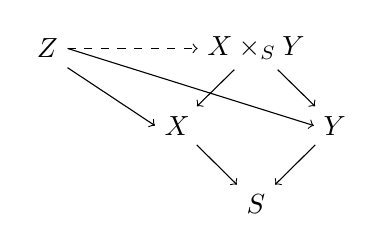
\begin{tikzpicture}[x=1cm,y=1cm]
\node (Z) at (-2.2,1.1) {$Z$};
\node (W) at (.45,1.1) {$X\times_S Y$};
\node (X) at (-.55,.12) {$X$};
\node (Y) at (1.45,.12) {$Y$};
\node (S) at (.45,-.87) {$S$};
\draw[->,dashed] (Z)--(W);
\draw[->] (W)--(X);
\draw[->] (W)--(Y);
\draw[->] (Z.south east)--(X.west);
\draw[->] (Z.east)--(Y.west);
\draw[->] (X)--(S);
\draw[->] (Y)--(S);
\end{tikzpicture}
\end{center}

If $X$ and $Y$ are schemes given without reference to any base scheme $S$, we take $S=\operatorname{Spec}\mathbb Z$ (Ex. \Goto{ex-II-2.5}{2.5}) and define the \emph{product} of $X$ and $Y$, denoted $X\times Y$, to be $X\times_{\operatorname{Spec}\mathbb Z}Y$.

\medskip
\noindent\hypertarget{result-II-3.3}{}\textbf{Theorem 3.3.} \emph{For any two schemes $X$ and $Y$ over a scheme $S$, the fibred product $X\times_S Y$ exists, and is unique up to unique isomorphism.}

\smallskip
\noindent\textsc{Proof.} The idea is first to construct products for affine schemes and then glue. We proceed in seven steps.

\hypertarget{proof-II-3.3-step-1}{}\emph{Step 1.} Let $X=\operatorname{Spec}A$, $Y=\operatorname{Spec}B$, $S=\operatorname{Spec}R$ all be affine. Then $A$ and $B$ are $R$-algebras, and I claim that $\operatorname{Spec}(A\otimes_R B)$ is a product for $X$ and $Y$ over $S$. Indeed, for any scheme $Z$, to give a morphism of $Z$ to $\operatorname{Spec}(A\otimes_R B)$ is the same as to give a homomorphism of the ring $A\otimes_R B$ into the ring $\Gamma(Z,\mathcal O_Z)$, by (Ex. \Goto{ex-II-2.4}{2.4}). But to give a homomorphism of $A\otimes_R B$ into any ring is the same as to give homomorphisms of $A$ and $B$ into that ring, inducing the same homomorphism on $R$. Applying (Ex. \Goto{ex-II-2.4}{2.4}) again, we see that to give a morphism of $Z$ into $\operatorname{Spec}(A\otimes_R B)$ is the same as giving morphisms of $Z$ into $X$ and into $Y$, which give rise to the same morphism of $Z$ into $S$. Thus $\operatorname{Spec}(A\otimes_R B)$ is the desired product.}
% Contents from body/page-102.tex.
\ChapterSheet{102}{88}{\Goto{p-74}{II\quad Schemes}}{%
\noindent\hypertarget{proof-II-3.3-step-2}{}\emph{Step 2.} It follows immediately from the universal property of the product that it is unique up to unique isomorphism, if it exists. We will need this uniqueness for those products already constructed, as we go along.

\hypertarget{proof-II-3.3-step-3}{}\emph{Step 3. Glueing morphisms.} We have already seen how to glue sheaves (Ex. \Goto{ex-II-1.22}{1.22}) and how to glue schemes (Ex. \Goto{ex-II-2.12}{2.12}). Now we glue morphisms. If $X$ and $Y$ are schemes, then to give a morphism $f$ from $X$ to $Y$, it is equivalent to give an open cover $\{U_i\}$ of $X$, together with morphisms $f_i\colon U_i\to Y$, where $U_i$ has the induced open subscheme structure, such that the restrictions of $f_i$ and $f_j$ to $U_i\cap U_j$ are the same, for each $i,j$. The proof is straightforward.

\hypertarget{proof-II-3.3-step-4}{}\emph{Step 4.} If $X,Y$ are schemes over a scheme $S$, if $U\subseteq X$ is an open subset, and if the product $X\times_S Y$ exists, then $p_1^{-1}(U)\subseteq X\times_S Y$ is a product for $U$ and $Y$ over $S$. Indeed, given a scheme $Z$, and morphisms $f\colon Z\to U$ and $g\colon Z\to Y$, $f$ determines a map of $Z$ to $X$ by composing with the inclusion $U\subseteq X$. Hence there is a map $\theta\colon Z\to X\times_S Y$ compatible with $f,g$ and the projections. But since $f(Z)\subseteq U$, we have $\theta(Z)\subseteq p_1^{-1}(U)$. So $\theta$ can be regarded as a morphism $Z\to p_1^{-1}(U)$. It is clearly unique, so $p_1^{-1}(U)$ is a product $U\times_S Y$.

\hypertarget{proof-II-3.3-step-5}{}\emph{Step 5.} Suppose given $X,Y$ schemes over $S$, suppose $\{X_i\}$ is an open covering of $X$, and suppose that for each $i$, $X_i\times_S Y$ exists. Then $X\times_S Y$ exists. Indeed, for each $i,j$, let $U_{ij}\subseteq X_i\times_S Y$ be $p_1^{-1}(X_{ij})$, where $X_{ij}=X_i\cap X_j$. Then by Step~\Goto{proof-II-3.3-step-4}{4}, $U_{ij}$ is a product for $X_{ij}$ and $Y$ over $S$. Hence by the uniqueness of products there are (unique) isomorphisms $\varphi_{ij}\colon U_{ij}\to U_{ji}$ for each $i,j$ compatible with all the projections. Furthermore, these isomorphisms are compatible with each other for each $i,j,k$, in the sense of (Ex. \Goto{ex-II-2.12}{2.12}). Thus we are in a position to glue the schemes $X_i\times_S Y$ via the isomorphisms $\varphi_{ij}$. We obtain by (Ex. \Goto{ex-II-2.12}{2.12}) a scheme $X\times_S Y$ which I claim is a product for $X$ and $Y$ over $S$. The projection morphisms $p_1$ and $p_2$ are defined by glueing the projections from the pieces $X_i\times_S Y$ (Step~\Goto{proof-II-3.3-step-3}{3}). Given a scheme $Z$ and morphisms $f\colon Z\to X$, $g\colon Z\to Y$, let $Z_i=f^{-1}(X_i)$. Then we get maps $\theta_i\colon Z_i\to X_i\times_S Y$, hence by composition with the inclusions $X_i\times_S Y\subseteq X\times_S Y$ we get maps $\theta_i\colon Z_i\to X\times_S Y$. One verifies that these maps agree on $Z_i\cap Z_j$, so we can glue the morphisms (Step~\Goto{proof-II-3.3-step-3}{3}) to obtain a morphism $\theta\colon Z\to X\times_S Y$, compatible with the projections and $f$ and $g$. The uniqueness of $\theta$ can be checked locally.

\hypertarget{proof-II-3.3-step-6}{}\emph{Step 6.} We know from Step~\Goto{proof-II-3.3-step-1}{1} that if $X,Y,S$ are all affine, then $X\times_S Y$ exists. Thus using Step~\Goto{proof-II-3.3-step-5}{5} we conclude that for any $X$, but $Y,S$ affine, the product exists. Using Step~\Goto{proof-II-3.3-step-5}{5} again, with $X$ and $Y$ interchanged, we find that the product exists for any $X$ and any $Y$ over an affine $S$.

\hypertarget{proof-II-3.3-step-7}{}\emph{Step 7.} Given arbitrary $X,Y,S$, let $q\colon X\to S$ and $r\colon Y\to S$ be the given morphisms. Let $S_i$ be an open affine cover of $S$. Let $X_i=q^{-1}(S_i)$ and let $Y_i=r^{-1}(S_i)$. Then by Step~\Goto{proof-II-3.3-step-6}{6}, $X_i\times_{S_i}Y_i$ exists. Note that this same scheme is a product for $X_i$ and $Y$ over $S$. Indeed, given morphisms $f\colon Z\to X_i$ and $g\colon Z\to Y$ over $S$, the image of $g$ must land inside $Y_i$. Thus $X_i\times_S Y$ exists for each $i$, and one more application of Step~\Goto{proof-II-3.3-step-5}{5} gives us $X\times_S Y$. This completes the proof.}
% Contents from body/page-103.tex.
\ChapterSheet{103}{89}{\Goto{sec-II-3}{3\quad First Properties of Schemes}}{%
Perhaps this is a good place to make some general remarks on the importance and uses of fibred products. To begin with, we can define the fibres of a morphism.

\medskip
\noindent\textbf{Definition.} Let $f\colon X\to Y$ be a morphism of schemes, and let $y\in Y$ be a point. Let $k(y)$ be the residue field of $y$, and let $\operatorname{Spec}k(y)\to Y$ be the natural morphism (Ex. \Goto{ex-II-2.7}{2.7}). Then we define the \emph{fibre} of the morphism $f$ over the point $y$ to be the scheme
\[
X_y=X\times_Y\operatorname{Spec}k(y).
\]

The fibre $X_y$ is a scheme over $k(y)$, and one can show that its underlying topological space is homeomorphic to the subset $f^{-1}(y)$ of $X$ (Ex. \Goto{ex-II-3.10}{3.10}).

The notion of the fibre of a morphism allows us to regard a morphism as a family of schemes (namely its fibres) parametrized by the points of the image scheme. Conversely, this notion of family is a good way of making sense of the idea of a family of schemes varying algebraically. For example, given a scheme $X_0$ over a field $k$, we define a \emph{family of deformations} of $X_0$ to be a morphism $f\colon X\to Y$ with $Y$ connected, together with a point $y_0\in Y$, such that $k(y_0)=k$, and $X_{y_0}\cong X_0$. The other fibres $X_y$ of $f$ are called \emph{deformations} of $X_0$.

An interesting kind of family arises when we have a scheme $X$ over $\operatorname{Spec}\mathbb Z$. In this case, taking the fibre over the generic point gives a scheme $X_{\mathbb Q}$ over $\mathbb Q$, while taking the fibre over a closed point, corresponding to a prime number $p$, gives a scheme $X_p$ over the finite field $\mathbb F_p$. We say that $X_p$ arises by \emph{reduction mod $p$} of the scheme $X$.

Another important application of fibred products is to the notion of \emph{base extension}. Let $S$ be a fixed scheme which we think of as a \emph{base scheme}, meaning that we are interested in the category of schemes over $S$. For example, think of $S=\operatorname{Spec}k$, where $k$ is a field. If $S'$ is another base scheme, and if $S'\to S$ is a morphism, then for any scheme $X$ over $S$, we let $X'=X\times_S S'$, which will be a scheme over $S'$. We say that $X'$ is obtained from $X$ by making a base extension $S'\to S$. For example, think of $S'=\operatorname{Spec}k'$ where $k'$ is an extension field of $k$. Note, by the way, that base extension is a transitive operation: if $S''\to S'\to S$ are two morphisms, then $(X\times_S S')\times_{S'}S''\cong X\times_S S''$.

This ties in with a general philosophy, emphasized by Grothendieck in his \textquotedblleft{}El\'ements de G\'eom\'etrie Alg\'ebrique\textquotedblright{} (\Goto{bib-EGA}{[EGA]}), that one should try to develop all concepts of algebraic geometry in a \emph{relative} context. Instead of always working over a fixed base field, and considering properties of one variety at a time, one should consider a morphism of schemes $f\colon X\to S$, and study properties of the morphism. It then becomes important to study the behavior of properties of $f$ under base extension, and in particular, to relate properties of $f$ to properties of the fibres of $f$. For example, if $f\colon X\to S$}
% Contents from body/page-104.tex.
\ChapterSheet{104}{90}{\Goto{p-74}{II\quad Schemes}}{%
\noindent is a morphism of finite type, and if $S'\to S$ is any base extension, then $f'\colon X'\to S'$ is also a morphism of finite type, where $X'=X\times_S S'$. Hence we say the property of a morphism $f$ being of finite type is \emph{stable under base extension}. On the other hand, if for example $f\colon X\to S$ is a morphism of integral schemes, the fibres of $f$ may be neither irreducible nor reduced. So the property of a scheme being integral is not stable under base extension.

\medskip
\noindent\hypertarget{result-II-3.3.1}{}\textbf{Example 3.3.1.} Let $k$ be an algebraically closed field, let
\[
X=\operatorname{Spec} k[x,y,t]/(ty-x^2),
\]
let $Y=\operatorname{Spec} k[t]$, and let $f\colon X\to Y$ be the morphism determined by the natural homomorphism $k[t]\to k[x,y,t]/(ty-x^2)$. Then $X$ and $Y$ are integral schemes of finite type over $k$, and $f$ is a surjective morphism. We identify the closed points of $Y$ with elements of $k$. For $a\in k$, $a\ne 0$, the fibre $X_a$ is the plane curve $ay=x^2$ in $\AffSpace[k]{2}$, which is an irreducible, reduced curve. But for $a=0$, the fibre $X_0$ is the nonreduced scheme given by $x^2=0$ in $\AffSpace{2}$. Thus we have a family (Fig.~\Goto{fig-book-7}{7}) in which most members are irreducible curves, but one is nonreduced. This shows how nonreduced schemes occur naturally even if one is primarily interested in varieties. We can say that the nonreduced scheme $x^2=0$ in $\AffSpace{2}$ is a deformation of the irreducible parabola $ay=x^2$ as $a\to 0$.

\smallskip
{\centering
\hypertarget{fig-book-7}{}%
\resizebox{.72\linewidth}{!}{%
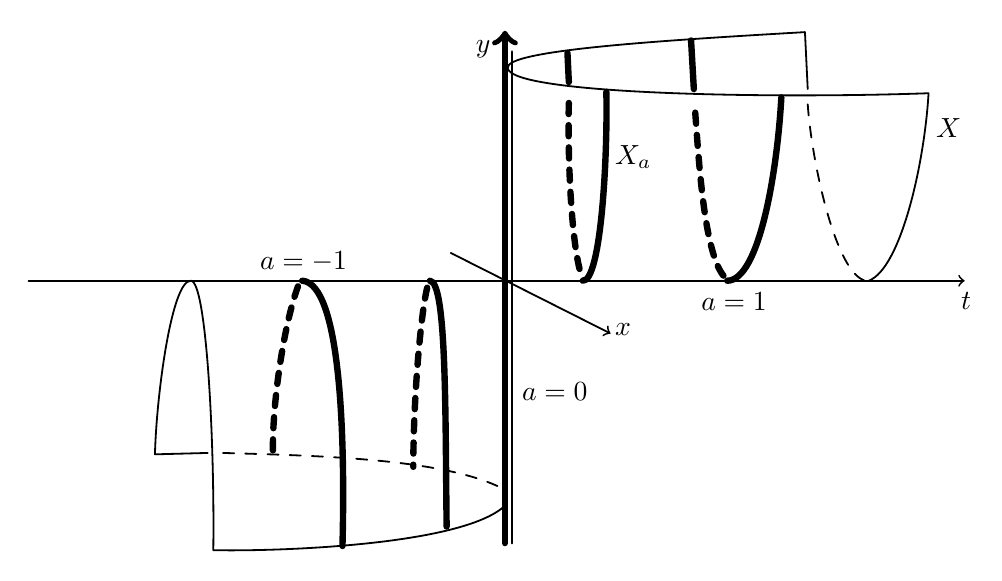
\begin{tikzpicture}[x=.5bp,y=-.5bp,line cap=round,line join=round,
    outline/.style={line width=.65bp},
    fibre/.style={line width=2.3bp},
    hidden/.style={dash pattern=on 4bp off 4bp},
    every node/.style={inner sep=1bp}]
  % Axes and the doubled line at a=0.
  \draw[outline,->] (18,195) -- (692,195);
  \draw[outline,->] (322,175) -- (437,233);
  \draw[line width=2.2bp,->] (361,384) -- (361,15);
  \draw[line width=.85bp] (366,384) -- (366,30);
  % Boundary and representative fibres for a>0.
  \draw[outline] (363,42) .. controls (360,29) and (474,22) .. (577,16)
    -- (579,57);
  \draw[outline] (363,42) .. controls (366,61) and (555,64) .. (666,60)
    .. controls (663,111) and (646,186) .. (623,195);
  \draw[outline,hidden] (579,68) .. controls (582,112) and (601,197) .. (623,195);
  \draw[fibre] (406,31) -- (407,52);
  \draw[fibre,hidden] (407,67) .. controls (406,109) and (409,174) .. (417,194);
  \draw[fibre] (434,59) .. controls (435,108) and (430,196) .. (417,195);
  \draw[fibre] (495,22) -- (497,57);
  \draw[fibre,hidden] (498,74) .. controls (501,114) and (505,182) .. (521,194);
  \draw[fibre] (560,63) .. controls (557,117) and (544,195) .. (521,195);
  % Boundary and representative fibres for a<0.
  \draw[outline] (109,320) .. controls (110,278) and (121,194) .. (135,195)
    .. controls (146,196) and (152,309) .. (151,389)
    .. controls (194,390) and (330,386) .. (361,357);
  \draw[outline] (109,320) -- (147,319);
  \draw[outline,hidden] (158,319) .. controls (227,321) and (318,323) .. (360,345);
  \draw[fibre,hidden] (212,199) .. controls (201,229) and (193,288) .. (194,320);
  \draw[fibre] (215,195) .. controls (243,197) and (246,309) .. (244,386);
  \draw[fibre,hidden] (305,200) .. controls (300,221) and (295,282) .. (295,329);
  \draw[fibre] (307,195) .. controls (319,196) and (318,289) .. (319,372);
  \node[above left] at (353,37) {$y$};
  \node[below] at (693,201) {$t$};
  \node[right] at (438,230) {$x$};
  \node[right] at (669,85) {$X$};
  \node[right] at (438,106) {$X_a$};
  \node[above] at (216,191) {$a=-1$};
  \node[below] at (526,201) {$a=1$};
  \node[right] at (371,275) {$a=0$};
\end{tikzpicture}}\par
\smallskip
\small\textbf{Figure 7.}\enspace An algebraic family of schemes.\par
}
\medskip
\noindent\hypertarget{result-II-3.3.2}{}\textbf{Example 3.3.2.} Similarly, if $X=\operatorname{Spec} k[x,y,t]/(xy-t)$, we get a family whose general member $X_a$ is an irreducible hyperbola $xy=a$, when $a\ne 0$, but whose special member $X_0$ is the reducible scheme $xy=0$ consisting of two lines.

\medskip
\noindent\textsc{Exercises}

\smallskip
\noindent\hypertarget{ex-II-3.1}{}\textbf{3.1.} Show that a morphism $f\colon X\to Y$ is locally of finite type if and only if for \emph{every} open affine subset $V=\operatorname{Spec} B$ of $Y$, $f^{-1}(V)$ can be covered by open affine subsets $U_j=\operatorname{Spec} A_j$, where each $A_j$ is a finitely generated $B$-algebra.}
% Contents from body/page-105.tex.
\ChapterSheet[10.3]{105}{91}{\Goto{sec-II-3}{3\quad First Properties of Schemes}}{%
\fontsize{9.5}{10.3}\selectfont%
\setlength{\parskip}{0pt}%
\setlength{\smallskipamount}{1.25pt}%
\noindent\hypertarget{ex-II-3.2}{}\textbf{3.2.} A morphism $f\colon X\to Y$ of schemes is \emph{quasi-compact} if there is a cover of $Y$ by open affines $V_i$ such that $f^{-1}(V_i)$ is quasi-compact for each $i$. Show that $f$ is quasi-compact if and only if for \emph{every} open affine subset $V\subseteq Y$, $f^{-1}(V)$ is quasi-compact.

\smallskip
\noindent\hypertarget{ex-II-3.3}{}\textbf{3.3.} (a) Show that a morphism $f\colon X\to Y$ is of finite type if and only if it is locally of finite type and quasi-compact.

\noindent\hangindent=3em\hspace*{1.7em}(b) Conclude from this that $f$ is of finite type if and only if for \emph{every} open affine subset $V=\operatorname{Spec} B$ of $Y$, $f^{-1}(V)$ can be covered by a finite number of open affines $U_j=\operatorname{Spec} A_j$, where each $A_j$ is a finitely generated $B$-algebra.

\noindent\hangindent=3em\hspace*{1.7em}(c) Show also if $f$ is of finite type, then for \emph{every} open affine subset $V=\operatorname{Spec} B\subseteq Y$, and for \emph{every} open affine subset $U=\operatorname{Spec} A\subseteq f^{-1}(V)$, $A$ is a finitely generated $B$-algebra.

\smallskip
\noindent\hypertarget{ex-II-3.4}{}\textbf{3.4.} Show that a morphism $f\colon X\to Y$ is finite if and only if for \emph{every} open affine subset $V=\operatorname{Spec} B$ of $Y$, $f^{-1}(V)$ is affine, equal to $\operatorname{Spec} A$, where $A$ is a finite $B$-module.

\smallskip
\noindent\hypertarget{ex-II-3.5}{}\textbf{3.5.} A morphism $f\colon X\to Y$ is \emph{quasi-finite} if for every point $y\in Y$, $f^{-1}(y)$ is a finite set.

\noindent\hangindent=3em\hspace*{1.7em}(a) Show that a finite morphism is quasi-finite.

\noindent\hangindent=3em\hspace*{1.7em}(b) Show that a finite morphism is \emph{closed}, i.e., the image of any closed subset is closed.

\noindent\hangindent=3em\hspace*{1.7em}(c) Show by example that a surjective, finite-type, quasi-finite morphism need not be finite.

\smallskip
\noindent\hypertarget{ex-II-3.6}{}\textbf{3.6.} Let $X$ be an integral scheme. Show that the local ring $\mathcal O_\xi$ of the generic point $\xi$ of $X$ is a field. It is called the \emph{function field} of $X$, and is denoted by $K(X)$. Show also that if $U=\operatorname{Spec} A$ is any \EditionText{nonempty }open affine subset of $X$, then $K(X)$ is isomorphic to the quotient field of $A$.

\smallskip
\noindent\hypertarget{ex-II-3.7}{}\textbf{3.7.} A morphism $f\colon X\to Y$, with $Y$ irreducible, is \emph{generically finite} if $f^{-1}(\eta)$ is a finite set, where $\eta$ is the generic point of $Y$. A morphism $f\colon X\to Y$ is \emph{dominant} if $f(X)$ is dense in $Y$. Now let $f\colon X\to Y$ be a dominant, generically finite morphism of finite type of integral schemes. Show that there is an open dense subset $U\subseteq Y$ such that the induced morphism $f^{-1}(U)\to U$ is finite. [\emph{Hint:} First show that the function field of $X$ is a finite field extension of the function field of $Y$.]

\smallskip
\noindent\hypertarget{ex-II-3.8}{}\textbf{3.8.} \emph{Normalization.} A scheme is \emph{normal} if all of its local rings are integrally closed domains. Let $X$ be an integral scheme. For each \EditionText{nonempty }open affine subset $U=\operatorname{Spec} A$ of $X$, let $\widetilde A$ be the integral closure of $A$ in its quotient field, and let $\widetilde U=\operatorname{Spec}\widetilde A$. Show that one can glue the schemes $\widetilde U$ to obtain a normal integral scheme $\widetilde X$, called the \emph{normalization} of $X$. Show also that there is a morphism $\widetilde X\to X$, having the following universal property: for every normal integral scheme $Z$, and for every dominant morphism $f\colon Z\to X$, $f$ factors uniquely through $\widetilde X$. If $X$ is of finite type over a field $k$, then the morphism $\widetilde X\to X$ is a finite morphism. This generalizes (I, Ex.~\Goto{ex-I-3.17}{3.17}).

\smallskip
\noindent\hypertarget{ex-II-3.9}{}\textbf{3.9.} \emph{The Topological Space of a Product.} Recall that in the category of varieties, the Zariski topology on the product of two varieties is not equal to the product topology (I, Ex.~\Goto{ex-I-1.4}{1.4}). Now we see that in the category of schemes, the underlying point set of a product of schemes is not even the product set.

\noindent\hangindent=3em\hspace*{1.7em}(a) Let $k$ be a field, and let $\AffSpace[k]{1}=\operatorname{Spec} k[x]$ be the affine line over $k$. Show that $\AffSpace[k]{1}\times_{\operatorname{Spec}k}\AffSpace[k]{1}\cong\AffSpace[k]{2}$, and show that the underlying point set of the product is not the product of the underlying point sets of the factors (even if $k$ is algebraically closed).}
% Contents from body/page-106.tex.
\ChapterSheet[10.5]{106}{92}{\Goto{p-74}{II\quad Schemes}}{%
\fontsize{9.5}{10.5}\selectfont%
\setlength{\parskip}{0pt}%
\setlength{\smallskipamount}{1.65pt}%
\noindent\hangindent=3em\hspace*{1.7em}(b) Let $k$ be a field, let $s$ and $t$ be indeterminates over $k$. Then $\operatorname{Spec} k(s)$, $\operatorname{Spec} k(t)$, and $\operatorname{Spec} k$ are all one-point spaces. Describe the product scheme $\operatorname{Spec} k(s)\times_{\operatorname{Spec}k} \operatorname{Spec} k(t)$.

\smallskip
\noindent\hypertarget{ex-II-3.10}{}\textbf{3.10.} \emph{Fibres of a Morphism.}

\noindent\hangindent=3em\hspace*{1.7em}(a) If $f\colon X\to Y$ is a morphism, and $y\in Y$ a point, show that $\operatorname{sp}(X_y)$ is homeomorphic to $f^{-1}(y)$ with the induced topology.

\noindent\hangindent=3em\hspace*{1.7em}(b) Let $X=\operatorname{Spec} k[s,t]/(s-t^2)$, let $Y=\operatorname{Spec} k[s]$, and let $f\colon X\to Y$ be the morphism defined by sending $s\to s$. If $y\in Y$ is the point $a\in k$ with $a\ne 0$, show that the fibre $X_y$ consists of two points, with residue field $k$. If $y\in Y$ corresponds to $0\in k$, show that the fibre $X_y$ is a nonreduced one-point scheme. If $\eta$ is the generic point of $Y$, show that $X_\eta$ is a one-point scheme, whose residue field is an extension of degree two of the residue field of $\eta$. (Assume $k$ algebraically closed\EditionText{ and $\operatorname{char} k\ne 2$}.)

\smallskip
\noindent\hypertarget{ex-II-3.11}{}\textbf{3.11.} \emph{Closed Subschemes.}

\noindent\hangindent=3em\hspace*{1.7em}(a) Closed immersions are stable under base extension: if $f\colon Y\to X$ is a closed immersion, and if $X'\to X$ is any morphism, then $f'\colon Y\times_X X'\to X'$ is also a closed immersion.

\noindent\hangindent=3em\hspace*{1.4em}*(b) If $Y$ is a closed subscheme of an affine scheme $X=\operatorname{Spec} A$, then $Y$ is also affine, and in fact $Y$ is the closed subscheme determined by a suitable ideal $\mathfrak a\subseteq A$ as the image of the closed immersion $\operatorname{Spec} A/\mathfrak a\to\operatorname{Spec} A$. [\emph{Hints:} First show that $Y$ can be covered by a finite number of open affine subsets of the form $D(f_i)\cap Y$, with $f_i\in A$. By adding some more $f_i$ with $D(f_i)\cap Y=\varnothing$, if necessary, show that we may assume that the $\{D(f_i)\}$ cover $X$. Next show that $f_1,\dots,f_r$ generate the unit ideal of $A$. Then use (Ex.~\Goto{ex-II-2.17}{2.17b}) to show that $Y$ is affine, and (Ex.~\Goto{ex-II-2.18}{2.18d}) to show that $Y$ comes from an ideal $\mathfrak a\subseteq A$.] \emph{Note:} We will give another proof of this result using sheaves of ideals later (\Goto{result-II-5.10}{5.10}).

\noindent\hangindent=3em\hspace*{1.7em}(c) Let $Y$ be a closed subset of a scheme $X$, and give $Y$ the reduced induced subscheme structure. If $Y'$ is any other closed subscheme of $X$ with the same underlying topological space, show that the closed immersion $Y\to X$ factors through $Y'$. We express this property by saying that the reduced induced structure is the smallest subscheme structure on a closed subset.

\noindent\hangindent=3em\hspace*{1.7em}(d) Let $f\colon Z\to X$ be a morphism. Then there is a unique closed subscheme $Y$ of $X$ with the following property: the morphism $f$ factors through $Y$, and if $Y'$ is any other closed subscheme of $X$ through which $f$ factors, then $Y\to X$ factors through $Y'$ also. We call $Y$ the \emph{scheme-theoretic image} of $f$. If $Z$ is a reduced scheme, then $Y$ is just the reduced induced structure on the closure of the image $f(Z)$.

\smallskip
\noindent\hypertarget{ex-II-3.12}{}\textbf{3.12.} \emph{Closed Subschemes of $\operatorname{Proj} S$.}

\noindent\hangindent=3em\hspace*{1.7em}(a) Let $\varphi\colon S\to T$ be a surjective homomorphism of graded rings, preserving degrees. Show that the open set $U$ of (Ex.~\Goto{ex-II-2.14}{2.14}) is equal to $\operatorname{Proj} T$, and the morphism $f\colon \operatorname{Proj} T\to\operatorname{Proj} S$ is a closed immersion.

\noindent\hangindent=3em\hspace*{1.7em}(b) If $I\subseteq S$ is a homogeneous ideal, take $T=S/I$ and let $Y$ be the closed subscheme of $X=\operatorname{Proj} S$ defined as image of the closed immersion $\operatorname{Proj} S/I\to X$. Show that different homogeneous ideals can give rise to the same closed subscheme. For example, let $d_0$ be an integer, and let $I'=\bigoplus_{d\ge d_0} I_d$. Show that $I$ and $I'$ determine the same closed subscheme.

We will see later (\Goto{result-II-5.16}{5.16}) that every closed subscheme of $X$ comes from a homogeneous ideal $I$ of $S$ (at least in the case where $S$ is a polynomial ring over $S_0$).}
% Contents from body/page-107.tex.
\ChapterSheet[10.5]{107}{93}{\Goto{sec-II-3}{3\quad First Properties of Schemes}}{%
\fontsize{9.5}{10.5}\selectfont%
\setlength{\parskip}{0pt}%
\setlength{\smallskipamount}{1.65pt}%
\noindent\hypertarget{ex-II-3.13}{}\textbf{3.13.} \emph{Properties of Morphisms of Finite Type.}

\noindent\hangindent=3em\hspace*{1.7em}(a) A closed immersion is a morphism of finite type.

\noindent\hangindent=3em\hspace*{1.7em}(b) A quasi-compact open immersion (Ex.~\Goto{ex-II-3.2}{3.2}) is of finite type.

\noindent\hangindent=3em\hspace*{1.7em}(c) A composition of two morphisms of finite type is of finite type.

\noindent\hangindent=3em\hspace*{1.7em}(d) Morphisms of finite type are stable under base extension.

\noindent\hangindent=3em\hspace*{1.7em}(e) If $X$ and $Y$ are schemes of finite type over $S$, then $X\times_S Y$ is of finite type over $S$.

\noindent\hangindent=3em\hspace*{1.7em}(f) If $X\xrightarrow{f}Y\xrightarrow{g}Z$ are two morphisms, and if $f$ is quasi-compact, and $g\circ f$ is of finite type, then $f$ is of finite type.

\noindent\hangindent=3em\hspace*{1.7em}(g) If $f\colon X\to Y$ is a morphism of finite type, and if $Y$ is noetherian, then $X$ is noetherian.

\smallskip
\noindent\hypertarget{ex-II-3.14}{}\textbf{3.14.} If $X$ is a scheme of finite type over a field, show that the closed points of $X$ are dense. Give an example to show that this is not true for arbitrary schemes.

\smallskip
\noindent\hypertarget{ex-II-3.15}{}\textbf{3.15.} Let $X$ be a scheme of finite type over a field $k$ (not necessarily algebraically closed).

\noindent\hangindent=3em\hspace*{1.7em}(a) Show that the following three conditions are equivalent (in which case we say that $X$ is \emph{geometrically irreducible}).

\noindent\hangindent=4.8em\hspace*{3em}(i) $X\times_k\bar k$ is irreducible, where $\bar k$ denotes the algebraic closure of $k$. (By abuse of notation, we write $X\times_k\bar k$ to denote $X\times_{\operatorname{Spec} k}\operatorname{Spec}\bar k$.)

\noindent\hangindent=4.8em\hspace*{3em}(ii) $X\times_k k_s$ is irreducible, where $k_s$ denotes the separable closure of $k$.

\noindent\hangindent=4.8em\hspace*{3em}(iii) $X\times_k K$ is irreducible for every extension field $K$ of $k$.

\noindent\hangindent=3em\hspace*{1.7em}(b) Show that the following three conditions are equivalent (in which case we say $X$ is \emph{geometrically reduced}).

\noindent\hangindent=4.8em\hspace*{3em}(i) $X\times_k\bar k$ is reduced.

\noindent\hangindent=4.8em\hspace*{3em}(ii) $X\times_k k_p$ is reduced, where $k_p$ denotes the perfect closure of $k$.

\noindent\hangindent=4.8em\hspace*{3em}(iii) $X\times_k K$ is reduced for all extension fields $K$ of $k$.

\noindent\hangindent=3em\hspace*{1.7em}(c) We say that $X$ is \emph{geometrically integral} if $X\times_k\bar k$ is integral. Give examples of integral schemes which are neither geometrically irreducible nor geometrically reduced.

\smallskip
\noindent\hypertarget{ex-II-3.16}{}\textbf{3.16.} \emph{Noetherian Induction.} Let $X$ be a noetherian topological space, and let $\mathcal P$ be a property of closed subsets of $X$. Assume that for any closed subset $Y$ of $X$, if $\mathcal P$ holds for every proper closed subset of $Y$, then $\mathcal P$ holds for $Y$. (In particular, $\mathcal P$ must hold for the empty set.) Then $\mathcal P$ holds for $X$.

\smallskip
\noindent\hypertarget{ex-II-3.17}{}\textbf{3.17.} \emph{Zariski Spaces.} A topological space $X$ is a \emph{Zariski space} if it is noetherian and every (nonempty) closed irreducible subset has a unique generic point (Ex.~\Goto{ex-II-2.9}{2.9}).

For example, let $R$ be a discrete valuation ring, and let $T=\operatorname{sp}(\operatorname{Spec} R)$. Then $T$ consists of two points $t_0=\text{the maximal ideal}$, $t_1=\text{the zero ideal}$. The open subsets are $\varnothing$, $\{t_1\}$, and $T$. This is an irreducible Zariski space with generic point $t_1$.

\noindent\hangindent=3em\hspace*{1.7em}(a) Show that if $X$ is a noetherian scheme, then $\operatorname{sp}(X)$ is a Zariski space.

\noindent\hangindent=3em\hspace*{1.7em}(b) Show that any minimal nonempty closed subset of a Zariski space consists of one point. We call these \emph{closed points}.

\noindent\hangindent=3em\hspace*{1.7em}(c) Show that a Zariski space $X$ satisfies the axiom $T_0$: given any two distinct points of $X$, there is an open set containing one but not the other.

\noindent\hangindent=3em\hspace*{1.7em}(d) If $X$ is an irreducible Zariski space, then its generic point is contained in every nonempty open subset of $X$.

\noindent\hangindent=3em\hspace*{1.7em}(e) If $x_0,x_1$ are points of a topological space $X$, and if $x_0\in\overline{\{x_1\}}$, then we say that $x_1$ \emph{specializes} to $x_0$, written $x_1\rightsquigarrow x_0$. We also say $x_0$ is a \emph{specialization}}
% Contents from body/page-108.tex.
\ChapterSheet[10.5]{108}{94}{\Goto{p-74}{II\quad Schemes}}{%
\fontsize{9.5}{10.5}\selectfont%
\setlength{\parskip}{0pt}%
\setlength{\smallskipamount}{1.65pt}%
\noindent\hangindent=3em\hspace*{3em}of $x_1$, or that $x_1$ is a \emph{generization} of $x_0$. Now let $X$ be a Zariski space. Show that the minimal points, for the partial ordering determined by $x_1>x_0$ if $x_1\rightsquigarrow x_0$, are the closed points, and the maximal points are the generic points of the irreducible components of $X$. Show also that a closed subset contains every specialization of any of its points. (We say closed subsets are \emph{stable under specialization}.) Similarly, open subsets are \emph{stable under generization}.

\noindent\hangindent=3em\hspace*{1.7em}(f) Let $t$ be the functor on topological spaces introduced in the proof of (\Goto{result-II-2.6}{2.6}). If $X$ is a noetherian topological space, show that $t(X)$ is a Zariski space. Furthermore $X$ itself is a Zariski space if and only if the map $\alpha\colon X\to t(X)$ is a homeomorphism.

\smallskip
\noindent\hypertarget{ex-II-3.18}{}\textbf{3.18.} \emph{Constructible Sets.} Let $X$ be a Zariski topological space. A \emph{constructible subset} of $X$ is a subset which belongs to the smallest family $\mathfrak F$ of subsets such that (1) every open subset is in $\mathfrak F$, (2) a finite intersection of elements of $\mathfrak F$ is in $\mathfrak F$, and (3) the complement of an element of $\mathfrak F$ is in $\mathfrak F$.

\noindent\hangindent=3em\hspace*{1.7em}(a) A subset of $X$ is \emph{locally closed} if it is the intersection of an open subset with a closed subset. Show that a subset of $X$ is constructible if and only if it can be written as a finite disjoint union of locally closed subsets.

\noindent\hangindent=3em\hspace*{1.7em}(b) Show that a constructible subset of an irreducible Zariski space $X$ is dense if and only if it contains the generic point. Furthermore, in that case it contains a nonempty open subset.

\noindent\hangindent=3em\hspace*{1.7em}(c) A subset $S$ of $X$ is closed if and only if it is constructible and stable under specialization. Similarly, a subset $T$ of $X$ is open if and only if it is constructible and stable under generization.

\noindent\hangindent=3em\hspace*{1.7em}(d) If $f\colon X\to Y$ is a continuous map of Zariski spaces, then the inverse image of any constructible subset of $Y$ is a constructible subset of $X$.

\smallskip
\noindent\hypertarget{ex-II-3.19}{}\textbf{3.19.} The real importance of the notion of constructible subsets derives from the following theorem of Chevalley---see Cartan and Chevalley \Goto{bib-474-9-item-1}{[1, expos\'e 7]} and see also Matsumura \Goto{bib-479-17}{[2, Ch.~2, \S6]}: let $f\colon X\to Y$ be a morphism of finite type of noetherian schemes. Then the image of any constructible subset of $X$ is a constructible subset of $Y$. In particular, $f(X)$, which need not be either open or closed, is a constructible subset of $Y$. Prove this theorem in the following steps.

\noindent\hangindent=3em\hspace*{1.7em}(a) Reduce to showing that $f(X)$ itself is constructible, in the case where $X$ and $Y$ are affine, integral noetherian schemes, and $f$ is a dominant morphism.

\noindent\hangindent=3em\hspace*{1.4em}*(b) In that case, show that $f(X)$ contains a nonempty open subset of $Y$ by using the following result from commutative algebra: let $A\subseteq B$ be an inclusion of noetherian integral domains, such that $B$ is a finitely generated $A$-algebra. Then given a nonzero element $b\in B$, there is a nonzero element $a\in A$ with the following property: if $\varphi\colon A\to K$ is any homomorphism of $A$ to an algebraically closed field $K$, such that $\varphi(a)\ne 0$, then $\varphi$ extends to a homomorphism $\varphi'$ of $B$ into $K$, such that $\varphi'(b)\ne 0$. [\emph{Hint:} Prove this algebraic result by induction on the number of generators of $B$ over $A$. For the case of one generator, prove the result directly. In the application, take $b=1$.]

\noindent\hangindent=3em\hspace*{1.7em}(c) Now use noetherian induction on $Y$ to complete the proof.

\noindent\hangindent=3em\hspace*{1.7em}(d) Give some examples of morphisms $f\colon X\to Y$ of varieties over an algebraically closed field $k$, to show that $f(X)$ need not be either open or closed.

\smallskip
\noindent\hypertarget{ex-II-3.20}{}\textbf{3.20.} \emph{Dimension.} Let $X$ be an integral scheme of finite type over a field $k$ (not necessarily algebraically closed). Use appropriate results from (I, \Goto{sec-I-1}{\S1}) to prove the following.}
% Contents from body/page-109.tex.
\BookMark{1}{2.4  Separated and Proper Morphisms}{sec-II-4}
\ChapterSheet{109}{95}{\Goto{sec-II-4}{4\quad Separated and Proper Morphisms}}{%
{\fontsize{9}{10.4}\selectfont
\begin{enumerate}[label=(\alph*),leftmargin=3.7em,topsep=0pt,nosep]
\item[\hypertarget{ex-II-3.20a}{}(a)] For any closed point $P\in X$, $\dim X=\dim\mathcal O_P$, where for rings, we always mean the Krull dimension.
\item[\hypertarget{ex-II-3.20b}{}(b)] Let $K(X)$ be the function field of $X$ (Ex.~\Goto{ex-II-3.6}{3.6}). Then $\dim X=\operatorname{tr.d.}K(X)/k$.
\item[(c)] If $Y$ is a closed subset of $X$, then $\operatorname{codim}(Y,X)=\inf\{\dim\mathcal O_{P,X}\mid P\in Y\}$.
\item[\hypertarget{ex-II-3.20d}{}(d)] If $Y$ is a \EditionText{nonempty }closed subset of $X$, then $\dim Y+\operatorname{codim}(Y,X)=\dim X$.
\item[\hypertarget{ex-II-3.20e}{}(e)] If $U$ is a nonempty open subset of $X$, then $\dim U=\dim X$.
\item[(f)] If $k\subseteq k'$ is a field extension, then every irreducible component of $X'=X\times_k k'$ has dimension $=\dim X$.
\end{enumerate}

\begin{description}[leftmargin=2.4em,labelindent=0pt,topsep=4pt,itemsep=4pt,parsep=0pt]
\item[\hypertarget{ex-II-3.21}{}\textbf{3.21.}] Let $R$ be a discrete valuation ring containing its residue field $k$. Let $X=\operatorname{Spec}R[t]$ be the affine line over $\operatorname{Spec}R$. Show that statements \Goto{ex-II-3.20a}{(a)}, \Goto{ex-II-3.20d}{(d)}, \Goto{ex-II-3.20e}{(e)} of (Ex.~\Goto{ex-II-3.20}{3.20}) are false for $X$.

\item[\hypertarget{ex-II-3.22}{}\textbf{*3.22.}] \emph{Dimension of the Fibres of a Morphism.} Let $f\colon X\to Y$ be a dominant morphism of integral schemes of finite type over a field $k$.
\begin{enumerate}[label=(\alph*),leftmargin=1.6em,nosep]
\item[\hypertarget{ex-II-3.22a}{}(a)] Let $Y'$ be a closed irreducible subset of $Y$, whose generic point $\eta'$ is contained in $f(X)$. Let $Z$ be any irreducible component of $f^{-1}(Y')$, such that $\eta'\in f(Z)$, and show that $\operatorname{codim}(Z,X)\leqslant\operatorname{codim}(Y',Y)$.
\item[\hypertarget{ex-II-3.22b}{}(b)] Let $e=\dim X-\dim Y$ be the \emph{relative dimension} of $X$ over $Y$. For any point $y\in f(X)$, show that every irreducible component of the fibre $X_y$ has dimension $\geqslant e$. [\emph{Hint:} Let $Y'=\{y\}^{-}$, and use \Goto{ex-II-3.22a}{(a)} and (Ex.~\Goto{ex-II-3.20b}{3.20b}).]
\item[\hypertarget{ex-II-3.22c}{}(c)] Show that there is a dense open subset $U\subseteq X$, such that for any $y\in f(U)$, $\dim U_y=e$. [\emph{Hint:} First reduce to the case where $X$ and $Y$ are affine, say $X=\operatorname{Spec}A$ and $Y=\operatorname{Spec}B$. Then $A$ is a finitely generated $B$-algebra. Take $t_1,\ldots,t_e\in A$ which form a transcendence base of $K(X)$ over $K(Y)$, and let $X_1=\operatorname{Spec}B[t_1,\ldots,t_e]$. Then $X_1$ is isomorphic to affine $e$-space over $Y$, and the morphism $X\to X_1$ is generically finite. Now use (Ex.~\Goto{ex-II-3.7}{3.7}) above.]
\item[(d)] Going back to our original morphism $f\colon X\to Y$, for any integer $h$, let $E_h$ be the set of points $x\in X$ such that, letting $y=f(x)$, there is an irreducible component $Z$ of the fibre $X_y$, containing $x$, and having $\dim Z\geqslant h$. Show that (1) $E_e=X$ (use \Goto{ex-II-3.22b}{(b)} above); (2) if $h>e$, then $E_h$ is not dense in $X$ (use \Goto{ex-II-3.22c}{(c)} above); and (3) $E_h$ is closed, for all $h$ (use induction on $\dim X$).
\item[(e)] Prove the following theorem of Chevalley---see Cartan and Chevalley \Goto{bib-474-9-item-1}{[1, expos\'e 8]}. For each integer $h$, let $C_h$ be the set of points $y\in Y$ such that $\dim X_y=h$. Then the subsets $C_h$ are constructible, and $C_e$ contains an open dense subset of $Y$.
\end{enumerate}

\item[\hypertarget{ex-II-3.23}{}\textbf{3.23.}] If $V,W$ are two varieties over an algebraically closed field $k$, and if $V\times W$ is their product, as defined in (I, Ex.~\Goto{ex-I-3.15}{3.15}, \Goto{ex-I-3.16}{3.16}), and if $t$ is the functor of \Goto{result-II-2.6}{(2.6)}, then $t(V\times W)=t(V)\times_{\operatorname{Spec}k}t(W)$.
\end{description}}

\medskip
\noindent\hypertarget{sec-II-4}{}\textbf{\large 4\quad Separated and Proper Morphisms}\par
\smallskip
\noindent We now come to two properties of schemes, or rather of morphisms between schemes, which correspond to well-known properties of ordinary topological spaces. Separatedness corresponds to the Hausdorff axiom for a topological space. Properness corresponds to the usual notion of properness, namely that the inverse image of a compact subset is compact. However, the usual definitions are not suitable in abstract algebraic geometry, because the Zariski topology \hypertarget{err-II-4-Hausdorff}{}\EditionText{need not be Hausdorff}, and the underlying topological space of a scheme
}
% Contents from body/page-110.tex.
\ChapterSheet{110}{96}{\Goto{p-74}{II\quad Schemes}}{%
\noindent does not accurately reflect all of its properties. So instead we will use definitions which reflect the functorial behavior of the morphism within the category of schemes. For schemes of finite type over $\mathbb C$, one can show that these notions, defined abstractly, are in fact the same as the usual notions if we consider those schemes as complex analytic spaces in the ordinary topology (\Goto{p-452}{Appendix B}).

In this section we will define separated and proper morphisms. We will give criteria for a morphism to be separated or proper using valuation rings. Then we will show that projective space over any scheme is proper.

\Dfn Let $f\colon X\to Y$ be a morphism of schemes. The \emph{diagonal morphism} is the unique morphism $\Delta\colon X\to X\times_Y X$ whose composition with both projection maps $p_1,p_2\colon X\times_Y X\to X$ is the identity map of $X\to X$. We say that the morphism $f$ is \emph{separated} if the diagonal morphism $\Delta$ is a closed immersion. In that case we also say $X$ is \emph{separated} over $Y$. A scheme $X$ is \emph{separated} if it is separated over $\operatorname{Spec}\mathbb Z$.

\medskip
\noindent\hypertarget{result-II-4.0}{}\hypertarget{result-II-4.0.1}{}\textbf{Example 4.0.1.} Let $k$ be a field, and let $X$ be the affine line with the origin doubled \Goto{result-II-2.3.6}{(2.3.6)}. Then $X$ is not separated over $k$. Indeed, $X\times_k X$ is the affine plane with doubled axes and four origins. The image of $\Delta$ is the usual diagonal, with two of those origins. This is not closed, because all four origins are in the closure of $\Delta(X)$.

\medskip
\noindent\hypertarget{result-II-4.0.2}{}\textbf{Example 4.0.2.} We will see later \Goto{result-II-4.10}{(4.10)} that if $V$ is any variety over an algebraically closed field $k$, then the associated scheme $t(V)$ is separated over $k$.

\medskip
\noindent\hypertarget{result-II-4.1}{}\textbf{Proposition 4.1.} \emph{If $f\colon X\to Y$ is any morphism of affine schemes, then $f$ is separated.}

\Proof Let $X=\operatorname{Spec}A$, $Y=\operatorname{Spec}B$. Then $A$ is a $B$-algebra, and $X\times_Y X$ is also affine, given by $\operatorname{Spec}A\otimes_B A$. The diagonal morphism $\Delta$ comes from the \emph{diagonal homomorphism} $A\otimes_B A\to A$ defined by $a\otimes a'\mapsto aa'$. This is a surjective homomorphism of rings, hence $\Delta$ is a closed immersion.

\medskip
\noindent\hypertarget{result-II-4.2}{}\textbf{Corollary 4.2.} \emph{An arbitrary morphism $f\colon X\to Y$ is separated if and only if the image of the diagonal morphism is a closed subset of $X\times_Y X$.}

\Proof One implication is obvious, so we have only to prove that if $\Delta(X)$ is a closed subset, then $\Delta\colon X\to X\times_Y X$ is a closed immersion. In other words, we have to check that $\Delta\colon X\to\Delta(X)$ is a homeomorphism, and that the morphism of sheaves $\mathcal O_{X\times_Y X}\to\Delta_*\mathcal O_X$ is surjective. Let $p_1\colon X\times_Y X\to X$ be the first projection. Since $p_1\circ\Delta=\operatorname{id}_X$, it follows immediately that $\Delta$ gives a homeomorphism onto $\Delta(X)$. To see that the map of sheaves $\mathcal O_{X\times_Y X}\to\Delta_*\mathcal O_X$ is surjective is a local question. For any point $P\in X$, let $U$ be an open affine
}
% Contents from body/page-111.tex.
\ChapterSheet{111}{97}{\Goto{sec-II-4}{4\quad Separated and Proper Morphisms}}{%
\noindent neighborhood of $P$ which is small enough so that $f(U)$ is contained in an open affine subset $V$ of $Y$. Then $U\times_V U$ is an open affine neighborhood of $\Delta(P)$, and by the proposition, $\Delta\colon U\to U\times_V U$ is a closed immersion. So our map of sheaves is surjective in a neighborhood of $P$, which completes the proof.

\medskip
Next we will discuss the valuative criterion of separatedness. The rough idea is that in order for a scheme $X$ to be separated, it should not contain any subscheme which looks like a curve with a doubled point, as in the example above. Another way of saying this is that if $C$ is a curve, and $P$ a point of $C$, then given any morphism of $C-P$ into $X$, it should admit at most one extension to a morphism of all of $C$ into $X$. (Compare (I, \Goto{result-I-6.8}{6.8}) where we showed that a projective variety has this property.)

In practice, this rough idea has to be modified. The question is local, so \hypertarget{err-II-4-curve-DVR}{}\EditionText{if $P$ is a nonsingular closed point of an integral curve, we replace the curve by its local ring at $P$, which is a discrete valuation ring.} Then since our schemes may be quite general, we must consider arbitrary (not necessarily discrete) valuation rings. Finally, we make the criterion relative over the image scheme $Y$ of a morphism.

See (I, \Goto{sec-I-6}{\S6}) for the definition and basic properties of valuation rings.

\medskip
\noindent\hypertarget{result-II-4.3}{}\textbf{Theorem 4.3} (Valuative Criterion of Separatedness). \emph{Let $f\colon X\to Y$ be a morphism of schemes, and assume that $X$ is noetherian. Then $f$ is separated if and only if the following condition holds. For any field $K$, and for any valuation ring $R$ with quotient field $K$, let $T=\operatorname{Spec}R$, let $U=\operatorname{Spec}K$, and let $i\colon U\to T$ be the morphism induced by the inclusion $R\subseteq K$. Given a morphism of $T$ to $Y$, and given a morphism of $U$ to $X$ which makes a commutative diagram
\[
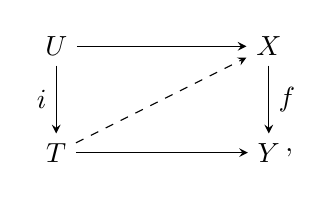
\begin{tikzpicture}[>=stealth]
\node (u) at (0,0) {$U$};
\node (x) at (2.7,0) {$X$};
\node (t) at (0,-1.35) {$T$};
\node (y) at (2.7,-1.35) {$Y$};
\draw[->] (u) -- (x);
\draw[->] (u) -- node[left] {$i$} (t);
\draw[->] (x) -- node[right] {$f$} (y);
\draw[->] (t) -- (y);
\draw[->,dashed] (t) -- (x);
\node[inner sep=0pt] at (2.96,-1.35) {$,$};
\end{tikzpicture}
\]
there is at most one morphism of $T$ to $X$ making the whole diagram commutative.}

\medskip
We will need two lemmas.

\medskip
\noindent\hypertarget{result-II-4.4}{}\textbf{Lemma 4.4.} \emph{Let $R$ be a valuation ring of a field $K$. Let $T=\operatorname{Spec}R$ and let $U=\operatorname{Spec}K$. To give a morphism of $U$ to a scheme $X$ is equivalent to giving a point $x_1\in X$ and an inclusion of fields $k(x_1)\subseteq K$. To give a morphism of $T$ to $X$ is equivalent to giving two points $x_0,x_1$ in $X$, with $x_0$ a specialization (see Ex.~\Goto{ex-II-3.17}{3.17e}) of $x_1$, and an inclusion of fields $k(x_1)\subseteq K$,}
}
% Contents from body/page-112.tex.
\ChapterSheet{112}{98}{\Goto{p-74}{II\quad Schemes}}{%
\noindent\emph{such that $R$ dominates the local ring $\mathcal O$ of $x_0$ on the subscheme $Z=\{x_1\}^{-}$ of $X$ with its reduced induced structure.}

\Proof $U$ is a one-point scheme, with structure sheaf $K$. To give a local homomorphism $\mathcal O_{x_1,X}\to K$ is the same as giving an inclusion of $k(x_1)\subseteq K$, so the first part is obvious. For the second part, let $t_0=\mathfrak m_R$ be the closed point of $T$, and let $t_1=(0)$ be the generic point of $T$. Given a morphism of $T$ to $X$, let $x_0$ and $x_1$ be the images of $t_0$ and $t_1$. Since $T$ is reduced, the morphism $T\to X$ factors through $Z$ (Ex.~\Goto{ex-II-3.11}{3.11}). Furthermore, $k(x_1)$ is the function field of $Z$. So we have a local homomorphism of $\mathcal O=\mathcal O_{x_0,Z}$ to $R$ compatible with the inclusion $k(x_1)\subseteq K$. In other words $R$ dominates $\mathcal O$.

Conversely, given the data consisting of $x_0,x_1$, and the inclusion $k(x_1)\subseteq K$ such that $R$ dominates $\mathcal O$, the inclusion $\mathcal O\to R$ gives a morphism $T\to\operatorname{Spec}\mathcal O$, which composed with the natural map $\operatorname{Spec}\mathcal O\to X$ gives the desired morphism $T\to X$.

\medskip
\noindent\hypertarget{result-II-4.5}{}\textbf{Lemma 4.5.} \emph{Let $f\colon X\to Y$ be a quasi-compact morphism of schemes (see Ex.~\Goto{ex-II-3.2}{3.2}). Then the subset $f(X)$ of $Y$ is closed if and only if it is stable under specialization (Ex.~\Goto{ex-II-3.17}{3.17e}).}

\Proof One implication is obvious, so we have only to show that if $f(X)$ is stable under specialization, then it is closed. Clearly we may assume that $X$ and $Y$ are both reduced, and that $f(X)^{-}=Y$ (replace $Y$ by the reduced induced structure on $f(X)^{-}$). So let $y\in Y$ be a point. We wish to show that $y\in f(X)$. Now we can replace $Y$ by an affine neighborhood of $y$, and so assume that $Y$ is affine. Then since $f$ is quasi-compact, $X$ will be a finite union of open affines $X_i$. We know that $y\in f(X)^{-}$. Hence $y\in f(X_i)^{-}$ for some $i$. Let $Y_i=f(X_i)^{-}$ with the reduced induced structure. Then $Y_i$ is also affine, and we will consider the dominant morphism $X_i\to Y_i$ of reduced affine schemes. Let $X_i=\operatorname{Spec}A$ and $Y_i=\operatorname{Spec}B$. Then the corresponding ring homomorphism $B\to A$ is injective, because the morphism is dominant. The point $y\in Y_i$ corresponds to a prime ideal $\mathfrak p\subseteq B$. Let $\mathfrak p'\subseteq\mathfrak p$ be a minimal prime ideal of $B$ contained in $\mathfrak p$. (Minimal prime ideals exist, by Zorn's lemma, because the intersection of any family of prime ideals, totally ordered by inclusion, is again a prime ideal!) Then $\mathfrak p'$ corresponds to a point $y'$ of $Y_i$ which specializes to $y$. I claim $y'\in f(X_i)$. Indeed, let us localize $A$ and $B$ at $\mathfrak p'$. Localization is an exact functor, so $B_{\mathfrak p'}\subseteq A\otimes B_{\mathfrak p'}$. Now $B_{\mathfrak p'}$ is a field. Let $\mathfrak q'_0$ be any prime ideal of $A\otimes B_{\mathfrak p'}$. Then $\mathfrak q'_0\cap B_{\mathfrak p'}=(0)$. Let $\mathfrak q'\subseteq A$ be the inverse image of $\mathfrak q'_0$ under the localization map $A\to A\otimes B_{\mathfrak p'}$. Then $\mathfrak q'\cap B=\mathfrak p'$. So $\mathfrak q'$ corresponds to a point $x'\in X_i$ with $f(x')=y'$. Now go back to the morphism $f\colon X\to Y$. We have $x'\in X$, $f(x')=y'$, so $y'\in f(X)$. But $f(X)$ is stable under specialization by hypothesis, and $y'\rightsquigarrow y$, so $y\in f(X)$, which is what we wanted to prove.

\smallskip
\noindent\textsc{Proof of Theorem \Goto{result-II-4.3}{4.3}.} First suppose $f$ is separated, and suppose given a diagram as above where there are two morphisms $h,h'$ of $T$ to $X$ making the whole diagram commutative.
}
% Contents from body/page-113.tex.
\ChapterSheet{113}{99}{\Goto{sec-II-4}{4\quad Separated and Proper Morphisms}}{%
\[
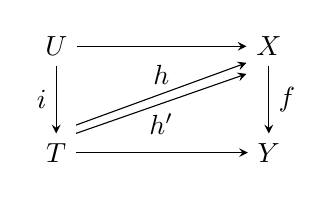
\begin{tikzpicture}[>=stealth]
\node (u) at (0,0) {$U$}; \node (x) at (2.7,0) {$X$};
\node (t) at (0,-1.35) {$T$}; \node (y) at (2.7,-1.35) {$Y$};
\draw[->] (u) -- (x);
\draw[->] (u) -- node[left] {$i$} (t);
\draw[->] (x) -- node[right] {$f$} (y);
\draw[->] (t) -- (y);
\draw[->] ([yshift=3pt]t.north east) -- node[above] {$h$} ([yshift=1pt]x.south west);
\draw[->] (t.north east) -- node[below] {$h'$} ([yshift=-3pt]x.south west);
\end{tikzpicture}
\]
\noindent Then we obtain a morphism $h''\colon T\to X\times_Y X$. Since the restrictions of $h$ and $h'$ to $U$ are the same, the generic point $t_1$ of $T$ has image in the diagonal $\Delta(X)$. Since $\Delta(X)$ is closed, the image of $t_0$ is also in the diagonal. Therefore $h$ and $h'$ both send the points $t_0,t_1$ to the same points $x_0,x_1$ of $X$. Since the inclusions of $k(x_1)\subseteq K$ induced by $h$ and $h'$ are also the same, it follows from \Goto{result-II-4.4}{(4.4)} that $h$ and $h'$ are equal.

Conversely, let us suppose the condition of the theorem satisfied. To show that $f$ is separated, it is sufficient by \Goto{result-II-4.2}{(4.2)} to show that $\Delta(X)$ is a closed subset of $X\times_Y X$. And since we have assumed that $X$ is noetherian, the morphism $\Delta$ is quasi-compact, so by \Goto{result-II-4.5}{(4.5)} it will be sufficient to show that $\Delta(X)$ is stable under specialization. So let $\xi_1\in\Delta(X)$ be a point, and let $\xi_1\rightsquigarrow\xi_0$ be a specialization. Let $K=k(\xi_1)$ and let $\mathcal O$ be the local ring of $\xi_0$ on the subscheme $\{\xi_1\}^{-}$ with its reduced induced structure. Then $\mathcal O$ is a local ring contained in $K$, so by (I, \Goto{result-I-6.1A}{6.1A}) there is a valuation ring $R$ of $K$ which dominates $\mathcal O$. Now by \Goto{result-II-4.4}{(4.4)} we obtain a morphism of $T=\operatorname{Spec}R$ to $X\times_Y X$ sending $t_0$ and $t_1$ to $\xi_0$ and $\xi_1$. Composing with the projections $p_1,p_2$ gives two morphisms of $T$ to $X$, which give the same morphism to $Y$, and whose restrictions to $U=\operatorname{Spec}K$ are the same, since $\xi_1\in\Delta(X)$. So by the condition, these two morphisms of $T$ to $X$ must be the same. Therefore the morphism $T\to X\times_Y X$ factors through the diagonal morphism $\Delta\colon X\to X\times_Y X$, and so $\xi_0\in\Delta(X)$. This completes the proof. Note in the last step it would not be sufficient to know only that $p_1(\xi_0)=p_2(\xi_0)$. For in general if $\xi\in X\times_Y X$ then $p_1(\xi)=p_2(\xi)$ does \emph{not} imply $\xi\in\Delta(X)$.

\medskip
\noindent\hypertarget{result-II-4.6}{}\textbf{Corollary 4.6.} \emph{Assume that all schemes are noetherian in the following statements.
\begin{enumerate}[label=(\alph*),leftmargin=2.4em,nosep]
\item Open and closed immersions are separated.
\item A composition of two separated morphisms is separated.
\item[\hypertarget{result-II-4.6c}{}(c)] Separated morphisms are stable under base extension.
\item[\hypertarget{result-II-4.6d}{}(d)] If $f\colon X\to Y$ and $f'\colon X'\to Y'$ are separated morphisms of schemes over a base scheme $S$, then the product morphism $f\times f'\colon X\times_S X'\to Y\times_S Y'$ is also separated.
\item[(e)] If $f\colon X\to Y$ and $g\colon Y\to Z$ are two morphisms and if $g\circ f$ is separated, then $f$ is separated.
\item[\hypertarget{result-II-4.6f}{}(f)] A morphism $f\colon X\to Y$ is separated if and only if $Y$ can be covered by open subsets $V_i$ such that $f^{-1}(V_i)\to V_i$ is separated for each $i$.
\end{enumerate}}

\Proof These statements all follow immediately from the condition of the theorem. We will give the proof of \Goto{result-II-4.6c}{(c)} to illustrate the method. Let $f\colon X\to Y$
}
% Contents from body/page-114.tex.
\ChapterSheet{114}{100}{\Goto{p-74}{II\quad Schemes}}{%
\noindent be a separated morphism, let $Y'\to Y$ be any morphism, and let $X'=X\times_Y Y'$ be obtained by base extension. We must show that $f'\colon X'\to Y'$ is separated. So suppose we are given morphisms of $T$ to $Y'$ and $U$ to $X'$ as in the theorem, and two morphisms of $T$ to $X'$ making the diagram
\[
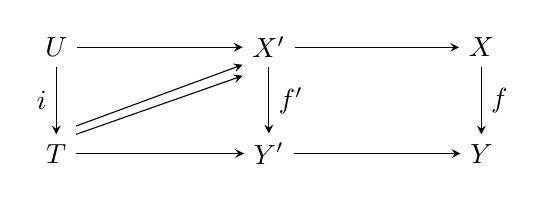
\begin{tikzpicture}[>=stealth]
\node (u) at (0,0) {$U$}; \node (xp) at (2.7,0) {$X'$}; \node (x) at (5.4,0) {$X$};
\node (t) at (0,-1.35) {$T$}; \node (yp) at (2.7,-1.35) {$Y'$}; \node (y) at (5.4,-1.35) {$Y$};
\draw[->] (u) -- (xp); \draw[->] (xp) -- (x);
\draw[->] (u) -- node[left] {$i$} (t);
\draw[->] (xp) -- node[right] {$f'$} (yp);
\draw[->] (x) -- node[right] {$f$} (y);
\draw[->] (t) -- (yp); \draw[->] (yp) -- (y);
\draw[->] ([yshift=3pt]t.north east) -- ([yshift=1pt]xp.south west);
\draw[->] (t.north east) -- ([yshift=-3pt]xp.south west);
\end{tikzpicture}
\]
\noindent commutative. Composing with the map $X'\to X$, we obtain two morphisms of $T$ to $X$. Since $f$ is separated, these are the same. But $X'$ is the fibred product of $X$ and $Y'$ over $Y$, so by the universal property of the fibred product, the two maps of $T$ to $X'$ are the same. Hence $f'$ is separated.

\medskip
\emph{Note on Noetherian Hypotheses.} You have probably noticed that in order to apply the theorem, it is not necessary to assume that all the schemes mentioned in the corollary are noetherian. In fact, even in the theorem itself, you can get by with assuming something less than $X$ noetherian (see Grothendieck \Goto{bib-EGA}{[EGA I, new ed., 5.5.4]}). My feeling is that if a noetherian hypothesis will make statements and proofs substantially simpler, then I will make that hypothesis, even though it may not be necessary. My justification for this attitude is that most of the motivation and examples in algebraic geometry come from schemes of finite type over a field, and constructions made from them, and practically all the schemes encountered in this way are noetherian. This attitude will prevail in \Goto{p-215}{Chapter III}, where noetherian hypotheses are built into the very foundations of our treatment of cohomology. The reader who wishes to avoid noetherian hypotheses is advised to read \Goto{bib-EGA}{[EGA]}, especially \Goto{bib-EGA}{[EGA IV, \S8]}.

\Dfn A morphism $f\colon X\to Y$ is \emph{proper} if it is separated, of finite type, and universally closed. Here we say that a morphism is \emph{closed} if the image of any closed subset is closed. A morphism $f\colon X\to Y$ is \emph{universally closed} if it is closed, and for any morphism $Y'\to Y$, the corresponding morphism $f'\colon X'\to Y'$ obtained by base extension is also closed.

\medskip
\noindent\hypertarget{result-II-4.6.1}{}\textbf{Example 4.6.1.} Let $k$ be a field and let $X$ be the affine line over $k$. Then $X$ is separated and of finite type over $k$, but it is not proper over $k$. Indeed, take the base extension \hypertarget{err-II-4-6-1}{}\EditionText{$X\to\operatorname{Spec}k$}. The map $X\times_k X\to X$ we obtain is the projection map of the affine plane onto the affine line. This is not a closed map. For example, the hyperbola given by the equation $xy=1$ is a closed subset of the plane, but its image under projection consists of the affine line minus the origin, which is not closed.

Of course it is clear that what is missing in this example is the point at infinity on the hyperbola. This suggests that the \emph{projective} line would be
}
% Contents from body/page-115.tex.
\ChapterSheet[10.6]{115}{101}{\Goto{sec-II-4}{4\quad Separated and Proper Morphisms}}{%
\noindent proper over $k$. In fact, we will see later \Goto{result-II-4.9}{(4.9)} that any projective variety over a field is proper.

\medskip
\noindent\hypertarget{result-II-4.7}{}\textbf{Theorem 4.7} (Valuative Criterion of Properness). \emph{Let $f\colon X\to Y$ be a morphism of finite type, with $X$ noetherian. Then $f$ is proper if and only if for every valuation ring $R$ and for every morphism of $U$ to $X$ and $T$ to $Y$ forming a commutative diagram
\[
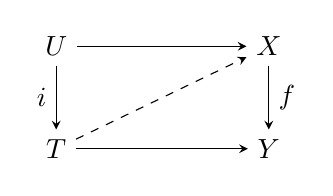
\begin{tikzpicture}[>=stealth]
\node (u) at (0,0) {$U$}; \node (x) at (2.7,0) {$X$};
\node (t) at (0,-1.3) {$T$}; \node (y) at (2.7,-1.3) {$Y$};
\draw[->] (u) -- (x);
\draw[->] (u) -- node[left] {$i$} (t);
\draw[->] (x) -- node[right] {$f$} (y);
\draw[->] (t) -- (y);
\draw[->,dashed] (t) -- (x);
\end{tikzpicture}
\]
(using the notation of \Goto{result-II-4.3}{(4.3)}), there exists a unique morphism $T\to X$ making the whole diagram commutative.}

\Proof First assume that $f$ is proper. Then by definition $f$ is separated, so the uniqueness of the morphism $T\to X$ will follow from \Goto{result-II-4.3}{(4.3)}, once we know it exists. For the existence, we consider the base extension $T\to Y$, and let $X_T=X\times_Y T$. We get a map $U\to X_T$ from the given maps $U\to X$ and $U\to T$.
\[
\begin{tikzpicture}[>=stealth]
\node (u) at (0,0) {$U$}; \node (xt) at (2.7,0) {$X_T$}; \node (x) at (5.4,0) {$X$};
\node (t) at (2.7,-1.3) {$T$}; \node (y) at (5.4,-1.3) {$Y$};
\draw[->] (u) -- (xt); \draw[->] (xt) -- (x);
\draw[->] (xt) -- node[left] {$f'$} (t);
\draw[->] (x) -- node[right] {$f$} (y);
\draw[->] (t) -- (y);
\end{tikzpicture}
\]
\noindent Let $\xi_1\in X_T$ be the image of the unique point $t_1$ of $U$. Let $Z=\{\xi_1\}^{-}$. Then $Z$ is a closed subset of $X_T$. Since $f$ is proper, it is universally closed, so the morphism $f'\colon X_T\to T$ must be closed, so $f'(Z)$ is a closed subset of $T$. But $f'(\xi_1)=t_1$, which is the generic point of $T$, so in fact $f'(Z)=T$. Hence there is a point $\xi_0\in Z$ with $f'(\xi_0)=t_0$. So we get a local homomorphism of local rings $R\to\mathcal O_{\xi_0,Z}$ corresponding to the morphism $f'$. Now the function field of $Z$ is $k(\xi_1)$, which is contained in $K$, by construction of $\xi_1$. By (I, \Goto{result-I-6.1A}{6.1A}), $R$ is maximal for the relation of domination between local subrings of $K$. Hence $R$ is isomorphic to $\mathcal O_{\xi_0,Z}$, and in particular $R$ dominates it. Hence by \Goto{result-II-4.4}{(4.4)} we obtain a morphism of $T$ to $X_T$ sending $t_0,t_1$ to $\xi_0,\xi_1$. Composing with the map $X_T\to X$ gives the desired morphism of $T$ to $X$.

Conversely, suppose the condition of the theorem holds. To show $f$ is proper, we have only to show that it is universally closed, since it is of finite type by hypothesis, and it is separated by \Goto{result-II-4.3}{(4.3)}. So let $Y'\to Y$ be any morphism, and let $f'\colon X'\to Y'$ be the morphism obtained from $f$ by base extension. Let $Z$ be a closed subset of $X'$, and give it the reduced induced structure.
}
% Contents from body/page-116.tex.
\ChapterSheet[10.6]{116}{102}{\Goto{p-74}{II\quad Schemes}}{%
\[
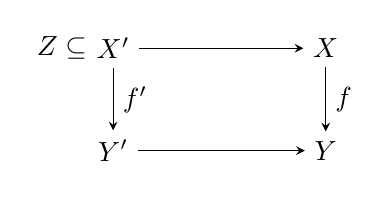
\begin{tikzpicture}[>=stealth]
\node at (-0.65,0) {$Z\subseteq$};
\node (xp) at (0,0) {$X'$}; \node (x) at (2.7,0) {$X$};
\node (yp) at (0,-1.3) {$Y'$}; \node (y) at (2.7,-1.3) {$Y$};
\draw[->] (xp) -- (x);
\draw[->] (xp) -- node[right] {$f'$} (yp);
\draw[->] (x) -- node[right] {$f$} (y);
\draw[->] (yp) -- (y);
\end{tikzpicture}
\]
\noindent We need to show that $f'(Z)$ is closed in $Y'$. Since $f$ is of finite type, so is $f'$ and so is the restriction of $f'$ to $Z$ (Ex.~\Goto{ex-II-3.13}{3.13}). In particular, the morphism $f'\colon Z\to Y'$ is quasi-compact, so by \Goto{result-II-4.5}{(4.5)} we have only to show that \hypertarget{err-II-4-7}{}\EditionText{$f'(Z)$} is stable under specialization. So let $z_1\in Z$ be a point, let $y_1=f'(z_1)$, and let $y_1\rightsquigarrow y_0$ be a specialization. Let $\mathcal O$ be the local ring of $y_0$ on $\{y_1\}^{-}$ with its reduced induced structure. Then the quotient field of $\mathcal O$ is $k(y_1)$, which is a subfield of $k(z_1)$. Let $K=k(z_1)$, and let $R$ be a valuation ring of $K$ which dominates $\mathcal O$ (which exists by (I, \Goto{result-I-6.1A}{6.1A})).

From this data, by \Goto{result-II-4.4}{(4.4)} we obtain morphisms $U\to Z$ and $T\to Y'$ forming a commutative diagram
\[
\begin{tikzpicture}[>=stealth]
\node (u) at (0,0) {$U$}; \node (z) at (2.7,0) {$Z$};
\node (t) at (0,-1.3) {$T$}; \node (yp) at (2.7,-1.3) {$Y'$};
\draw[->] (u) -- (z);
\draw[->] (u) -- node[left] {$i$} (t);
\draw[->] (z) -- (yp);
\draw[->] (t) -- (yp);
\node[inner sep=0pt] at (2.99,-1.3) {$.$};
\end{tikzpicture}
\]
\noindent Composing with the morphisms $Z\to X'\to X$ and $Y'\to Y$, we get morphisms $U\to X$ and $T\to Y$ to which we can apply the condition of the theorem. So there is a morphism of $T\to X$ making the diagram commute. Since $X'$ is a fibred product, it lifts to give a morphism $T\to X'$. And since $Z$ is closed, and the generic point of $T$ goes to $z_1\in Z$, this morphism factors to give a morphism $T\to Z$. Now let $z_0$ be the image of $t_0$. Then $f'(z_0)=y_0$, so $y_0\in f'(Z)$. This completes the proof.

\medskip
\noindent\hypertarget{result-II-4.8}{}\textbf{Corollary 4.8.} \emph{In the following statements, we take all schemes to be noetherian.
\begin{enumerate}[label=(\alph*),leftmargin=2.4em,nosep]
\item A closed immersion is proper.
\item A composition of proper morphisms is proper.
\item Proper morphisms are stable under base extension.
\item Products of proper morphisms are proper as in \Goto{result-II-4.6d}{(4.6d)}.
\item[\hypertarget{result-II-4.8e}{}(e)] If $f\colon X\to Y$ and $g\colon Y\to Z$ are two morphisms, if $g\circ f$ is proper, and if $g$ is separated, then $f$ is proper.
\item[(f)] Properness is local on the base as in \Goto{result-II-4.6f}{(4.6f)}.
\end{enumerate}}

\Proof These results follow immediately from the condition of the theorem, taking into account (Ex.~\Goto{ex-II-3.13}{3.13}) which deals with the finite type property, and \Goto{result-II-4.6}{(4.6)}. We will give the proof of \Goto{result-II-4.8e}{(e)} to illustrate the method. Assume $g\circ f$ is proper and $g$ is separated. Then $f$ is of finite type by (Ex.~\Goto{ex-II-3.13}{3.13}). (We have assumed that $X$ is noetherian, so $f$ is automatically quasi-compact.) Also $f$ is separated by \Goto{result-II-4.6}{(4.6)}. So we have to show that given a valuation ring $R$, and morphisms $U\to X$ and $T\to Y$ making a commutative diagram,
}
% Contents from body/page-117.tex.
\ChapterSheet[10.9]{117}{103}{\Goto{sec-II-4}{4\quad Separated and Proper Morphisms}}{%
\[
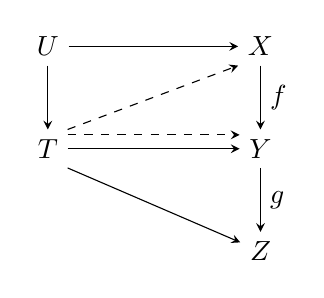
\begin{tikzpicture}[>=stealth]
\node (u) at (0,0) {$U$}; \node (x) at (2.7,0) {$X$};
\node (t) at (0,-1.3) {$T$}; \node (y) at (2.7,-1.3) {$Y$};
\node (z) at (2.7,-2.6) {$Z$};
\draw[->] (u) -- (x);
\draw[->] (u) -- (t);
\draw[->] (x) -- node[right] {$f$} (y);
\draw[->] (y) -- node[right] {$g$} (z);
\draw[->] (t) -- (y);
\draw[->] (t.south east) -- (z);
\draw[->,dashed] ([yshift=5pt]t.east) -- ([yshift=5pt]y.west);
\draw[->,dashed] (t.north east) -- (x.south west);
\end{tikzpicture}
\]
\noindent then there exists a morphism of $T$ to $X$ making the diagram commutative.

Let $T\to Z$ be the composed map. Then since $g\circ f$ is proper, there is a map of $T$ to $X$ commuting with the map of $T\to Z$. By composing with $f$, we get a second map of $T$ to $Y$. But now since $g$ is separated, the two maps of $T$ to $Y$ are the same, so we are done.

\medskip
Our next objective is to define projective morphisms and to show that any projective morphism is proper. Recall that in \Goto{sec-II-2}{Section 2} we defined projective $n$-space $\Proj_A^n$ over any ring $A$ to be $\operatorname{Proj}A[x_0,\ldots,x_n]$. Note that if $A\to B$ is a homomorphism of rings, and $\operatorname{Spec}B\to\operatorname{Spec}A$ is the corresponding morphism of affine schemes, then $\Proj_B^n\cong\Proj_A^n\times_{\operatorname{Spec}A}\operatorname{Spec}B$. In particular, for any ring $A$, we have $\Proj_A^n\cong\Proj_{\mathbb Z}^n\times_{\operatorname{Spec}\mathbb Z}\operatorname{Spec}A$. This motivates the following definition for any scheme $Y$.

\Dfn If $Y$ is any scheme, we define \emph{projective $n$-space} over $Y$, denoted $\Proj_Y^n$, to be $\Proj_{\mathbb Z}^n\times_{\operatorname{Spec}\mathbb Z}Y$. A morphism $f\colon X\to Y$ of schemes is \emph{projective} if it factors into a closed immersion $i\colon X\to\Proj_Y^n$ for some $n$, followed by the projection $\Proj_Y^n\to Y$. A morphism $f\colon X\to Y$ is \emph{quasi-projective} if it factors into an open immersion $j\colon X\to X'$ followed by a projective morphism $g\colon X'\to Y$. (This definition of projective morphism is slightly different from the one in Grothendieck \Goto{bib-EGA}{[EGA II, 5.5]}. The two definitions are equivalent in case $Y$ itself is quasi-projective over an affine scheme.)

\smallskip
\noindent\hypertarget{result-II-4.8.1}{}\textbf{Example 4.8.1.} Let $A$ be a ring, let $S$ be a graded ring with $S_0=A$, which is finitely generated as an $A$-algebra by $S_1$. Then the natural map $\operatorname{Proj}S\to\operatorname{Spec}A$ is a projective morphism. Indeed, by hypothesis $S$ is a quotient of a polynomial ring $S'=A[x_0,\ldots,x_n]$. The surjective homomorphism of graded rings $S'\to S$ gives rise to a closed immersion $\operatorname{Proj}S\to\operatorname{Proj}S'=\Proj_A^n$, which shows that $\operatorname{Proj}S$ is projective over $A$ (Ex.~\Goto{ex-II-3.12}{3.12}).

\medskip
\noindent\hypertarget{result-II-4.9}{}\textbf{Theorem 4.9.} \emph{A projective morphism of noetherian schemes is proper. A quasi-projective morphism of noetherian schemes is of finite type and separated.}

\Proof Taking into account the results of (Ex.~\Goto{ex-II-3.13}{3.13}) and \Goto{result-II-4.6}{(4.6)} and \Goto{result-II-4.8}{(4.8)}, it will be sufficient to show that $X=\Proj_{\mathbb Z}^n$ is proper over $\operatorname{Spec}\mathbb Z$. Recall by \Goto{result-II-2.5}{(2.5)} that $X$ is a union of open affine subsets $V_i=D_+(x_i)$, and that $V_i$ is
}
% Contents from body/page-118.tex.
\ChapterSheet{118}{104}{\Goto{p-74}{II\quad Schemes}}{%
\noindent isomorphic to $\operatorname{Spec}\mathbb Z[x_0/x_i,\ldots,x_n/x_i]$. Thus $X$ is of finite type. To show that $X$ is proper, we will use the criterion of \Goto{result-II-4.7}{(4.7)} and imitate the proof of (I, \Goto{result-I-6.8}{6.8}). So suppose given a valuation ring $R$ and morphisms $U\to X$, $T\to\operatorname{Spec}\mathbb Z$ as shown:
\[
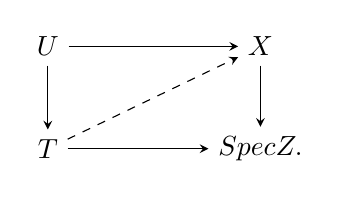
\begin{tikzpicture}[>=stealth]
\node (u) at (0,0) {$U$}; \node (x) at (2.7,0) {$X$};
\node (t) at (0,-1.3) {$T$}; \node (z) at (2.7,-1.3) {$\operatorname{Spec}\mathbb Z.$};
\draw[->] (u) -- (x);
\draw[->] (u) -- (t);
\draw[->] (x) -- (z);
\draw[->] (t) -- (z);
\draw[->,dashed] (t) -- (x);
\end{tikzpicture}
\]
\noindent Let $\xi_1\in X$ be the image of the unique point of $U$. Using induction on $n$, we may assume that $\xi_1$ is not contained in any of the hyperplanes $X-V_i$, which are each isomorphic to $\Proj^{n-1}$. In other words, we may assume that $\xi_1\in\bigcap V_i$, and hence all of the functions $x_i/x_j$ are invertible elements of the local ring $\mathcal O_{\xi_1}$.

We have an inclusion $k(\xi_1)\subseteq K$ given by the morphism $U\to X$. Let $f_{ij}\in K$ be the image of $x_i/x_j$. Then the $f_{ij}$ are nonzero elements of $K$, and $f_{ik}=f_{ij}\cdot f_{jk}$ for all $i,j,k$. Let \hypertarget{err-II-4-9-valuation}{}\EditionText{$v\colon K^\times\to G$} be the valuation associated to the valuation ring $R$. Let $g_i=v(f_{i0})$ for $i=0,\ldots,n$. Choose $k$ such that $g_k$ is minimal among the set $\{g_0,\ldots,g_n\}$, for the ordering of $G$. Then for each $i$ we have
\[
v(f_{ik})=g_i-g_k\geqslant0,
\]
hence $f_{ik}\in R$ for $i=0,\ldots,n$. Then we can define a homomorphism
\[
\varphi\colon\mathbb Z[x_0/x_k,\ldots,x_n/x_k]\to R
\]
by sending $x_i/x_k$ to $f_{ik}$. It is compatible with the given field inclusion $k(\xi_1)\subseteq K$. This homomorphism $\varphi$ gives a morphism $T\to V_k$, and hence a morphism of $T$ to $X$ which is the one required. The uniqueness of this morphism follows from the construction and the way the $V_i$ patch together.

\medskip
\noindent\hypertarget{result-II-4.10}{}\textbf{Proposition 4.10.} \emph{Let $k$ be an algebraically closed field. The image of the functor $t\colon\mathfrak{Var}(k)\to\mathfrak{Sch}(k)$ of \Goto{result-II-2.6}{(2.6)} is exactly the set of quasi-projective integral schemes over $k$. The image of the set of projective varieties is the set of projective integral schemes. In particular, for any variety $V$, $t(V)$ is an integral, separated scheme of finite type over $k$.}

\Proof We have already seen in \Goto{sec-II-3}{Section 3} that for any variety $V$, the associated scheme $t(V)$ is integral and of finite type over $k$. Since varieties were defined as locally closed subsets of projective space (I, \Goto{sec-I-3}{\S3}), it is clear that $t(V)$ is also quasi-projective.

For the converse, it will be sufficient to show that any projective integral scheme $Y$ over $k$ is in the image of $t$. Let $Y$ be a closed subscheme of $\Proj_k^n$, and let $V$ be the set of closed points of $Y$. Then $V$ is a closed subset of the \emph{variety} $\Proj^n$. Since $V$ is dense in $Y$ (Ex.~\Goto{ex-II-3.14}{3.14}) we see that $V$ is irreducible, so $V$ is a projective variety, and we see also that $t(V)$ and $Y$ have the same
}
% Contents from body/page-119.tex.
\ChapterSheet{119}{105}{\Goto{sec-II-4}{4\quad Separated and Proper Morphisms}}{%
\noindent underlying topological space. But they are both reduced closed subschemes of $\Proj_k^n$, so they are isomorphic (Ex.~\Goto{ex-II-3.11}{3.11}).

\Dfn An \emph{abstract variety} is an integral separated scheme of finite type over an algebraically closed field $k$. If it is proper over $k$, we will also say it is \emph{complete}.

\medskip
\noindent\hypertarget{result-II-4.10.1}{}\textbf{Remark 4.10.1.} From now on we will use the word \textquotedblleft{}variety\textquotedblright{} to mean \textquotedblleft{}abstract variety\textquotedblright{} in the sense just defined. We will identify the varieties of \Goto{p-15}{Chapter I} with their associated schemes, and refer to them as quasi-projective varieties. We will use the words \textquotedblleft{}curve,\textquotedblright{} \textquotedblleft{}surface,\textquotedblright{} \textquotedblleft{}three-fold,\textquotedblright{} etc., to mean an abstract variety of dimension $1$, $2$, $3$, etc.

\medskip
\noindent\hypertarget{result-II-4.10.2}{}\textbf{Remark 4.10.2.} The concept of an abstract variety was invented by Weil \Goto{bib-483-4}{[1]}. He needed it to provide a purely algebraic construction of the Jacobian variety of a curve, which at first appeared only as an abstract variety (Weil \Goto{bib-weil-2}{[2]}). Then Chow \Goto{bib-chow-3}{[3]} gave a different construction of the Jacobian variety showing that it was in fact a projective variety. Later Weil \Goto{bib-weil-6}{[6]} himself showed that all abelian varieties were projective.

Meanwhile Nagata \Goto{bib-480-9}{[1]} found an example of a complete abstract nonprojective variety, showing that in fact the new class of abstract varieties is larger than the class of projective varieties.

We can sum up the present state of knowledge of this subject as follows.
\begin{enumerate}[label=(\alph*),leftmargin=1.6em,nosep]
\item Every complete curve is projective (III, Ex.~\Goto{ex-III-5.8}{5.8}).
\item Every nonsingular complete surface is projective (Zariski \Goto{bib-483-15}{[5]}). See also Hartshorne \Goto{legacy-b-h5}{[5, II.4.2]}.
\item There exist singular nonprojective complete surfaces (Nagata \Goto{bib-480-11}{[3]}). See also (Ex.~\Goto{ex-II-7.13}{7.13}) and (III, Ex.~\Goto{ex-III-5.9}{5.9}).
\item There exist nonsingular complete nonprojective three-folds (Nagata \Goto{bib-480-12}{[4]}, Hironaka \Goto{bib-477-13}{[2]}, and (\Goto{p-452}{Appendix B})).
\item Every variety can be embedded as an open dense subset of a complete variety (Nagata \Goto{bib-480-13}{[6]}).
\end{enumerate}

\smallskip
The following algebraic result will be used in (Ex.~\Goto{ex-II-4.6}{4.6}).

\medskip
\noindent\hypertarget{result-II-4.11A}{}\textbf{Theorem 4.11A.} \emph{If $A$ is a subring of a field $K$, then the integral closure of $A$ in $K$ is the intersection of all valuation rings of $K$ which contain $A$.}

\Proof Bourbaki \Goto{bib-474-4-item-1}{[1, Ch.~VI, \S1, no.~3, Thm.~3, p.~92]}.

\Exercises
{\fontsize{9}{10.5}\selectfont
\begin{description}[leftmargin=2.4em,labelindent=0pt,topsep=0pt,itemsep=4pt,parsep=0pt]
\item[\hypertarget{ex-II-4.1}{}\textbf{4.1.}] Show that a finite morphism is proper.
\item[\hypertarget{ex-II-4.2}{}\textbf{4.2.}] Let $S$ be a scheme, let $X$ be a reduced scheme over $S$, and let $Y$ be a separated scheme over $S$. Let $f$ and $g$ be two $S$-morphisms of $X$ to $Y$ which agree on an open dense subset of $X$. Show that $f=g$. Give examples to show that this
\end{description}}
}
% Contents from body/page-120.tex.
\ChapterSheet{120}{106}{\Goto{p-74}{II\quad Schemes}}{%
\fontsize{9}{10.5}\selectfont
\noindent\hangindent=2.4em\hangafter=0\hspace*{2.4em}result fails if either (a) $X$ is nonreduced, or (b) $Y$ is nonseparated. [\emph{Hint:} Consider the map $h\colon X\to Y\times_S Y$ obtained from $f$ and $g$.]\par

\begin{description}[leftmargin=2.4em,labelindent=0pt,topsep=3pt,itemsep=4pt,parsep=0pt]
\item[\hypertarget{ex-II-4.3}{}\textbf{4.3.}] Let $X$ be a separated scheme over an affine scheme $S$. Let $U$ and $V$ be open affine subsets of $X$. Then $U\cap V$ is also affine. Give an example to show that this fails if $X$ is not separated.

\item[\hypertarget{ex-II-4.4}{}\textbf{4.4.}] Let $f\colon X\to Y$ be a morphism of separated schemes of finite type over a noetherian scheme $S$. Let $Z$ be a closed subscheme of $X$ which is proper over $S$. Show that $f(Z)$ is closed in $Y$, and that $f(Z)$ with its image subscheme structure (Ex.~\Goto{ex-II-3.11}{3.11d}) is proper over $S$. We refer to this result by saying that \textquotedblleft{}the image of a proper scheme is proper.\textquotedblright{} [\emph{Hint:} Factor $f$ into the graph morphism $\Gamma_f\colon X\to X\times_S Y$ followed by the second projection $p_2$, and show that $\Gamma_f$ is a closed immersion.]

\item[\hypertarget{ex-II-4.5}{}\textbf{4.5.}] Let $X$ be an integral scheme of finite type over a field $k$, having function field $K$. We say that a valuation of $K/k$ (see I, \Goto{sec-I-6}{\S6}) has \emph{center} $x$ on $X$ if its valuation ring $R$ dominates the local ring $\mathcal O_{x,X}$.
\begin{enumerate}[label=(\alph*),leftmargin=1.6em,nosep]
\item[\hypertarget{ex-II-4.5a}{}(a)] If $X$ is separated over $k$, then the center of any valuation of $K/k$ on $X$ (if it exists) is unique.
\item[\hypertarget{ex-II-4.5b}{}(b)] If $X$ is proper over $k$, then every valuation of $K/k$ has a unique center on $X$.
\item[*(c)] Prove the converses of \Goto{ex-II-4.5a}{(a)} and \Goto{ex-II-4.5b}{(b)}. [\emph{Hint:} While parts \Goto{ex-II-4.5a}{(a)} and \Goto{ex-II-4.5b}{(b)} follow quite easily from \Goto{result-II-4.3}{(4.3)} and \Goto{result-II-4.7}{(4.7)}, their converses will require some comparison of valuations in different fields.]
\item[(d)] If $X$ is proper over $k$, and if $k$ is algebraically closed, show that $\Gamma(X,\mathcal O_X)=k$. This result generalizes (I, \Goto{result-I-3.4}{3.4a}). [\emph{Hint:} Let $a\in\Gamma(X,\mathcal O_X)$, with $a\notin k$. Show that there is a valuation ring $R$ of $K/k$ with $a^{-1}\in\mathfrak m_R$. Then use \Goto{ex-II-4.5b}{(b)} to get a contradiction.]
\end{enumerate}
\emph{Note.} If $X$ is a variety over $k$, the criterion of \Goto{ex-II-4.5b}{(b)} is sometimes taken as the definition of a complete variety.

\item[\hypertarget{ex-II-4.6}{}\textbf{4.6.}] Let $f\colon X\to Y$ be a proper morphism of affine varieties over $k$. Then $f$ is a finite morphism. [\emph{Hint:} Use \Goto{result-II-4.11A}{(4.11A)}.]

\item[\hypertarget{ex-II-4.7}{}\textbf{4.7.}] \emph{Schemes Over $\mathbb R$.} For any scheme $X_0$ over $\mathbb R$, let $X=X_0\times_{\mathbb R}\mathbb C$. Let $\alpha\colon\mathbb C\to\mathbb C$ be complex conjugation, and let $\sigma\colon X\to X$ be the automorphism obtained by keeping $X_0$ fixed and applying $\alpha$ to $\mathbb C$. Then $X$ is a scheme over $\mathbb C$, and $\sigma$ is a \emph{semi-linear} automorphism, in the sense that we have a commutative diagram
\[
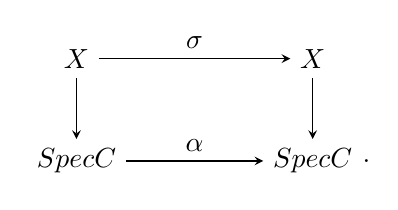
\begin{tikzpicture}[>=stealth]
\node (x1) at (0,0) {$X$}; \node (x2) at (3,0) {$X$};
\node (c1) at (0,-1.3) {$\operatorname{Spec}\mathbb C$};
\node (c2) at (3,-1.3) {$\operatorname{Spec}\mathbb C$};
\draw[->] (x1) -- node[above] {$\sigma$} (x2);
\draw[->] (x1) -- (c1);
\draw[->] (x2) -- (c2);
\draw[->] (c1) -- node[above] {$\alpha$} (c2);
\node[inner sep=0pt] at ([xshift=1.6pt]c2.east) {$.$};
\end{tikzpicture}
\]
\noindent Since $\sigma^2=\operatorname{id}$, we call $\sigma$ an \emph{involution}.
\begin{enumerate}[label=(\alph*),leftmargin=1.6em,nosep]
\item[\hypertarget{ex-II-4.7a}{}(a)] Now let $X$ be a separated scheme of finite type over $\mathbb C$, let $\sigma$ be a semilinear involution on $X$, and assume that for any two points $x_1,x_2\in X$, there is an open affine subset containing both of them. (This last condition is satisfied for example if $X$ is quasi-projective.) Show that there is a unique separated scheme $X_0$ of finite type over $\mathbb R$, such that $X_0\times_{\mathbb R}\mathbb C\cong X$, and such that this isomorphism identifies the given involution of $X$ with the one on $X_0\times_{\mathbb R}\mathbb C$ described above.
\end{enumerate}
\end{description}
}
% Contents from body/page-121.tex.
\ChapterSheet{121}{107}{\Goto{sec-II-4}{4\quad Separated and Proper Morphisms}}{%
\fontsize{9}{10.5}\selectfont
\noindent\hangindent=4em\hangafter=0\hspace*{5em}For the following statements, $X_0$ will denote a separated scheme of finite type over $\mathbb R$, and $X,\sigma$ will denote the corresponding scheme with involution over $\mathbb C$.\par
\begin{enumerate}[label=(\alph*),start=2,leftmargin=4em,nosep]
\item Show that $X_0$ is affine if and only if $X$ is.
\item If $X_0,Y_0$ are two such schemes over $\mathbb R$, then to give a morphism $f_0\colon X_0\to Y_0$ is equivalent to giving a morphism $f\colon X\to Y$ which commutes with the involutions, i.e., $f\circ\sigma_X=\sigma_Y\circ f$.
\item If $X\cong\AffSpace[\mathbb C]{1}$, then $X_0\cong\AffSpace[\mathbb R]{1}$.
\item If $X\cong\Proj_{\mathbb C}^{1}$, then either $X_0\cong\Proj_{\mathbb R}^{1}$, or $X_0$ is isomorphic to the conic in $\Proj_{\mathbb R}^{2}$ given by the homogeneous equation $x_0^2+x_1^2+x_2^2=0$.
\end{enumerate}

\begin{description}[leftmargin=2.4em,labelindent=0pt,topsep=4pt,itemsep=4pt,parsep=0pt]
\item[\hypertarget{ex-II-4.8}{}\textbf{4.8.}] Let $\mathcal P$ be a property of morphisms of schemes such that:
\begin{enumerate}[label=(\alph*),leftmargin=1.6em,nosep]
\item a closed immersion has $\mathcal P$;
\item a composition of two morphisms having $\mathcal P$ has $\mathcal P$;
\item $\mathcal P$ is stable under base extension.\par
Then show that:
\item a product of morphisms having $\mathcal P$ has $\mathcal P$;
\item[\hypertarget{ex-II-4.8e}{}(e)] if $f\colon X\to Y$ and $g\colon Y\to Z$ are two morphisms, and if $g\circ f$ has $\mathcal P$ and $g$ is separated, then $f$ has $\mathcal P$;
\item[(f)] If $f\colon X\to Y$ has $\mathcal P$, then $f_{\mathrm{red}}\colon X_{\mathrm{red}}\to Y_{\mathrm{red}}$ has $\mathcal P$.\par
[\emph{Hint:} For \Goto{ex-II-4.8e}{(e)}, consider the graph morphism $\Gamma_f\colon X\to X\times_Z Y$ and note that it is obtained by base extension from the diagonal morphism $\Delta\colon Y\to Y\times_Z Y$.]
\end{enumerate}

\item[\hypertarget{ex-II-4.9}{}\textbf{4.9.}] Show that a composition of projective morphisms is projective. [\emph{Hint:} Use the Segre embedding defined in (I, Ex.~\Goto{ex-I-2.14}{2.14}) and show that it gives a closed immersion $\Proj^r\times\Proj^s\to\Proj^{rs+r+s}$.] Conclude that projective morphisms have properties (a)--(f) of (Ex.~\Goto{ex-II-4.8}{4.8}) above.

\item[\hypertarget{ex-II-4.10}{}\textbf{*4.10.}] \emph{Chow's Lemma.} This result says that proper morphisms are fairly close to projective morphisms. Let $X$ be proper over a noetherian scheme $S$. Then there is a scheme $X'$ and a morphism $g\colon X'\to X$ such that $X'$ is projective over $S$, and there is an open dense subset $U\subseteq X$ such that $g$ induces an isomorphism of $g^{-1}(U)$ to $U$. Prove this result in the following steps.
\begin{enumerate}[label=(\alph*),leftmargin=1.6em,nosep]
\item Reduce to the case $X$ irreducible.
\item Show that $X$ can be covered by a finite number of open subsets $U_i$, $i=1,\ldots,n$, each of which is quasi-projective over $S$. Let $U_i\to P_i$ be an open immersion of $U_i$ into a scheme $P_i$ which is projective over $S$.
\item Let $U=\bigcap U_i$, and consider the map
\[
f\colon U\to X\times_S P_1\times_S\cdots\times_S P_n
\]
deduced from the given maps $U\to X$ and $U\to P_i$. Let $X'$ be the closed image subscheme structure (Ex.~\Goto{ex-II-3.11}{3.11d}) $f(U)^{-}$. Let $g\colon X'\to X$ be the projection onto the first factor, and let $h\colon X'\to P=P_1\times_S\cdots\times_S P_n$ be the projection onto the product of the remaining factors. Show that $h$ is a closed immersion, hence $X'$ is projective over $S$.
\item Show that $g^{-1}(U)\to U$ is an isomorphism, thus completing the proof.
\end{enumerate}

\item[\hypertarget{ex-II-4.11}{}\textbf{4.11.}] If you are willing to do some harder commutative algebra, and stick to noetherian schemes, then we can express the valuative criteria of separatedness and properness using only \emph{discrete} valuation rings.
\begin{enumerate}[label=(\alph*),leftmargin=1.6em,nosep]
\item If \hypertarget{err-II-4-11a}{}\EditionText{$(\mathcal O,\mathfrak m)$ is a noetherian local domain of positive dimension} with quotient field $K$, and if $L$ is a finitely generated field extension of $K$, then there exists a discrete valuation ring $R$ of
\end{enumerate}
\end{description}
}
% Contents from body/page-122.tex.
\BookMark{1}{2.5  Sheaves of Modules}{sec-II-5}
\ChapterSheet{122}{108}{\Goto{p-74}{II\quad Schemes}}{%
{\fontsize{9}{10.5}\selectfont
\noindent\hangindent=4em\hangafter=0\hspace*{4em}$L$ dominating $\mathcal O$. Prove this in the following steps. By taking a polynomial ring over $\mathcal O$, reduce to the case where $L$ is a \emph{finite} extension field of $K$. Then show that for a suitable choice of generators $x_1,\ldots,x_n$ of $\mathfrak m$, the ideal $\mathfrak a=(x_1)$ in $\mathcal O'=\mathcal O[x_2/x_1,\ldots,x_n/x_1]$ is not equal to the unit ideal. Then let $\mathfrak p$ be a minimal prime ideal of $\mathfrak a$, and let $\mathcal O'_{\mathfrak p}$ be the localization of $\mathcal O'$ at $\mathfrak p$. This is a noetherian local domain of dimension $1$ dominating $\mathcal O$. Let $\widetilde{\mathcal O}'_{\mathfrak p}$ be the integral closure of $\mathcal O'_{\mathfrak p}$ in $L$. Use the theorem of Krull--Akizuki (see Nagata \Goto{bib-480-14}{[7, p.~115]}) to show that $\widetilde{\mathcal O}'_{\mathfrak p}$ is noetherian of dimension $1$. Finally, take $R$ to be a localization of $\widetilde{\mathcal O}'_{\mathfrak p}$ at one of its maximal ideals.\par
\begin{enumerate}[label=(\alph*),start=2,leftmargin=4em,nosep]
\item Let $f\colon X\to Y$ be a morphism of finite type of noetherian schemes. Show that $f$ is separated (respectively, proper) if and only if the criterion of \Goto{result-II-4.3}{(4.3)} (respectively, \Goto{result-II-4.7}{(4.7)}) holds for all \emph{discrete} valuation rings.
\end{enumerate}

\begin{description}[leftmargin=2.4em,labelindent=0pt,topsep=4pt,itemsep=4pt,parsep=0pt]
\item[\hypertarget{ex-II-4.12}{}\textbf{4.12.}] \emph{Examples of Valuation Rings.} Let $k$ be an algebraically closed field.
\begin{enumerate}[label=(\alph*),leftmargin=1.6em,nosep]
\item If $K$ is a function field of dimension $1$ over $k$ (I, \Goto{sec-I-6}{\S6}), then every valuation ring of $K/k$ (except for $K$ itself) is discrete. Thus the set of all of them is just the abstract nonsingular curve $C_K$ of (I, \Goto{sec-I-6}{\S6}).
\item If $K/k$ is a function field of dimension two, there are several different kinds of valuations. Suppose that $X$ is a complete nonsingular surface with function field $K$.
\begin{enumerate}[label=(\arabic*),leftmargin=1.6em,nosep]
\item If $Y$ is an irreducible curve on $X$, with generic point $x_1$, then the local ring $R=\mathcal O_{x_1,X}$ is a discrete valuation ring of $K/k$ with center at the (nonclosed) point $x_1$ on $X$.
\item If $f\colon X'\to X$ is a birational morphism\EditionText{ of varieties}, and if $Y'$ is an irreducible curve in $X'$ whose image in $X$ is a single closed point $x_0$, then \hypertarget{err-II-4-12b2}{}\EditionText{assuming $X'$ is normal at the generic point of $Y'$, }the local ring $R$ of the generic point of $Y'$ on $X'$ is a discrete valuation ring of $K/k$ with center at the closed point $x_0$ on $X$.
\item[\hypertarget{ex-II-4.12b3}{}(3)] Let $x_0\in X$ be a closed point. Let $f\colon X_1\to X$ be the blowing-up of $x_0$ (I, \Goto{sec-I-4}{\S4}) and let $E_1=f^{-1}(x_0)$ be the exceptional curve. Choose a closed point $x_1\in E_1$, let $f_2\colon X_2\to X_1$ be the blowing-up of $x_1$, and let $E_2=f_2^{-1}(x_1)$ be the exceptional curve. Repeat. In this manner we obtain a sequence of varieties $X_i$ with closed points $x_i$ chosen on them, and for each $i$, the local ring $\mathcal O_{x_{i+1},X_{i+1}}$ dominates $\mathcal O_{x_i,X_i}$. Let $R_0=\bigcup_{i=0}^{\infty}\mathcal O_{x_i,X_i}$. Then $R_0$ is a local ring, so it is dominated by some valuation ring $R$ of $K/k$ by (I, \Goto{result-I-6.1A}{6.1A}). Show that $R$ is a valuation ring of $K/k$, and that it has center $x_0$ on $X$. When is $R$ a discrete valuation ring?
\end{enumerate}
\end{enumerate}
\emph{Note.} We will see later (V, Ex.~\Goto{ex-V-5.6}{5.6}) that in fact the $R_0$ of \Goto{ex-II-4.12b3}{(3)} is already a valuation ring itself, so $R_0=R$. Furthermore, every valuation ring of $K/k$ (except for $K$ itself) is one of the three kinds just described.
\end{description}}

\medskip
\noindent\hypertarget{sec-II-5}{}\textbf{\large 5\quad Sheaves of Modules}\par
\smallskip
\noindent So far we have discussed schemes and morphisms between them without mentioning any sheaves other than the structure sheaves. We can increase the flexibility of our technique enormously by considering sheaves of modules on a given scheme. Especially important are quasi-coherent and coherent sheaves, which play the role of modules (respectively, finitely generated modules) over a ring.
}
% Contents from body/page-123.tex.
\ChapterSheet{123}{109}{\Goto{sec-II-5}{5\quad Sheaves of Modules}}{%
\indent In this section we will develop the basic properties of quasi-coherent and coherent sheaves. In particular we will introduce the important \textquotedblleft{}twisting sheaf\textquotedblright{} $\mathcal O(1)$ of Serre on a projective scheme.

We will start by defining sheaves of modules on a ringed space.

\medskip
\noindent\textbf{Definitions.} Let $(X,\mathcal O_X)$ be a ringed space (see \Goto{sec-II-2}{\S2}). A \emph{sheaf of $\mathcal O_X$-modules} (or simply an \emph{$\mathcal O_X$-module}) is a sheaf $\mathcal F$ on $X$, such that for each open set $U\subseteq X$, the group $\mathcal F(U)$ is an $\mathcal O_X(U)$-module, and for each inclusion of open sets $V\subseteq U$, the restriction homomorphism $\mathcal F(U)\to\mathcal F(V)$ is compatible with the module structures via the ring homomorphism $\mathcal O_X(U)\to\mathcal O_X(V)$. A \emph{morphism} $\mathcal F\to\mathcal G$ of sheaves of $\mathcal O_X$-modules is a morphism of sheaves, such that for each open set $U\subseteq X$, the map $\mathcal F(U)\to\mathcal G(U)$ is a homomorphism of $\mathcal O_X(U)$-modules.

Note that the kernel, cokernel, and image of a morphism of $\mathcal O_X$-modules is again an $\mathcal O_X$-module. If $\mathcal F'$ is a subsheaf of $\mathcal O_X$-modules of an $\mathcal O_X$-module $\mathcal F$, then the quotient sheaf $\mathcal F/\mathcal F'$ is an $\mathcal O_X$-module. Any direct sum, direct product, direct limit, or inverse limit of $\mathcal O_X$-modules is an $\mathcal O_X$-module. If $\mathcal F$ and $\mathcal G$ are two $\mathcal O_X$-modules, we denote the group of morphisms from $\mathcal F$ to $\mathcal G$ by $\operatorname{Hom}_{\mathcal O_X}(\mathcal F,\mathcal G)$, or sometimes $\operatorname{Hom}_X(\mathcal F,\mathcal G)$ or $\operatorname{Hom}(\mathcal F,\mathcal G)$ if no confusion can arise. A sequence of $\mathcal O_X$-modules and morphisms is \emph{exact} if it is exact as a sequence of sheaves of abelian groups.

If $U$ is an open subset of $X$, and if $\mathcal F$ is an $\mathcal O_X$-module, then $\mathcal F|_U$ is an $\mathcal O_X|_U$-module. If $\mathcal F$ and $\mathcal G$ are two $\mathcal O_X$-modules, the presheaf
\[
U\mapsto\operatorname{Hom}_{\mathcal O_X|_U}(\mathcal F|_U,\mathcal G|_U)
\]
is a sheaf, which we call the \emph{sheaf $\mathcal H\!om$} (Ex.~\Goto{ex-II-1.15}{1.15}), and denote by $\mathcal H\!om_{\mathcal O_X}(\mathcal F,\mathcal G)$. It is also an $\mathcal O_X$-module.

We define the \emph{tensor product} $\mathcal F\otimes_{\mathcal O_X}\mathcal G$ of two $\mathcal O_X$-modules to be the sheaf associated to the presheaf $U\mapsto\mathcal F(U)\otimes_{\mathcal O_X(U)}\mathcal G(U)$. We will often write simply $\mathcal F\otimes\mathcal G$ with $\mathcal O_X$ understood.

An $\mathcal O_X$-module $\mathcal F$ is \emph{free} if it is isomorphic to a direct sum of copies of $\mathcal O_X$. It is \emph{locally free} if $X$ can be covered by open sets $U$ for which $\mathcal F|_U$ is a free $\mathcal O_X|_U$-module. In that case the \emph{rank} of $\mathcal F$ on \EditionText{such a nonempty open set is the number of copies of the structure sheaf needed (finite or infinite), provided every stalk of $\mathcal O_X$ is nonzero. Under this hypothesis, if $X$ is connected, the rank of a locally free sheaf is the same everywhere.} A locally free sheaf of rank $1$ is also called an \emph{invertible sheaf}.

A \emph{sheaf of ideals} on $X$ is a sheaf of modules $\mathcal I$ which is a subsheaf of $\mathcal O_X$. In other words, for every open set $U$, $\mathcal I(U)$ is an ideal in $\mathcal O_X(U)$.

Let $f\colon(X,\mathcal O_X)\to(Y,\mathcal O_Y)$ be a morphism of ringed spaces (see \Goto{sec-II-2}{\S2}). If $\mathcal F$ is an $\mathcal O_X$-module, then $f_*\mathcal F$ is an $f_*\mathcal O_X$-module. Since we have the morphism $f^\#\colon\mathcal O_Y\to f_*\mathcal O_X$ of sheaves of rings on $Y$, this gives $f_*\mathcal F$ a natural structure of $\mathcal O_Y$-module. We call it the \emph{direct image} of $\mathcal F$ by the morphism $f$.

Now let $\mathcal G$ be a sheaf of $\mathcal O_Y$-modules. Then $f^{-1}\mathcal G$ is an $f^{-1}\mathcal O_Y$-module. Because of the adjoint property of $f^{-1}$ (Ex.~\Goto{ex-II-1.18}{1.18}) we have a morphism
}
% Contents from body/page-124.tex.
\ChapterSheet{124}{110}{\Goto{p-74}{II\quad Schemes}}{%
{\leftskip=12pt\relax
\noindent $f^{-1}\mathcal O_Y\to\mathcal O_X$ of sheaves of rings on $X$. We define $f^*\mathcal G$ to be the tensor product
\[
f^{-1}\mathcal G\otimes_{f^{-1}\mathcal O_Y}\mathcal O_X.
\]
Thus $f^*\mathcal G$ is an $\mathcal O_X$-module. We call it the \emph{inverse image} of $\mathcal G$ by the morphism $f$.

As in (Ex.~\Goto{ex-II-1.18}{1.18}) one can show that $f_*$ and $f^*$ are adjoint functors between the category of $\mathcal O_X$-modules and the category of $\mathcal O_Y$-modules. To be precise, for any $\mathcal O_X$-module $\mathcal F$ and any $\mathcal O_Y$-module $\mathcal G$, there is a natural isomorphism of groups
\[
\operatorname{Hom}_{\mathcal O_X}(f^*\mathcal G,\mathcal F)\cong
\operatorname{Hom}_{\mathcal O_Y}(\mathcal G,f_*\mathcal F).
\]\par}

Now that we have the general notion of a sheaf of modules on a ringed space, we specialize to the case of schemes. We start by defining the sheaf of modules $\widetilde M$ on $\operatorname{Spec}A$ associated to a module $M$ over a ring $A$.

\medskip
\noindent\textbf{Definition.} Let $A$ be a ring and let $M$ be an $A$-module. We define the \emph{sheaf associated} to $M$ on $\operatorname{Spec}A$, denoted by $\widetilde M$, as follows. For each prime ideal $\mathfrak p\subseteq A$, let $M_{\mathfrak p}$ be the localization of $M$ at $\mathfrak p$. For any open set $U\subseteq\operatorname{Spec}A$ we define the group $\widetilde M(U)$ to be the set of functions $s\colon U\to\coprod_{\mathfrak p\in U}M_{\mathfrak p}$ such that for each $\mathfrak p\in U$, $s(\mathfrak p)\in M_{\mathfrak p}$, and such that $s$ is locally a fraction $m/f$ with $m\in M$ and $f\in A$. To be precise, we require that for each $\mathfrak p\in U$, there is a neighborhood $V$ of $\mathfrak p$ in $U$, and there are elements $m\in M$ and $f\in A$, such that for each $\mathfrak q\in V$, $f\notin\mathfrak q$, and $s(\mathfrak q)=m/f$ in $M_{\mathfrak q}$. We make $\widetilde M$ into a sheaf by using the obvious restriction maps.

\medskip
\noindent\hypertarget{result-II-5.1}{}\textbf{Proposition 5.1.} \emph{Let $A$ be a ring, let $M$ be an $A$-module, and let $\widetilde M$ be the sheaf on $X=\operatorname{Spec}A$ associated to $M$. Then:}
\par{\itshape\leftskip=12pt
\hypertarget{result-II-5.1a}{}(a) $\widetilde M$ is an $\mathcal O_X$-module;

\hypertarget{result-II-5.1b}{}(b) for each $\mathfrak p\in X$, the stalk $(\widetilde M)_{\mathfrak p}$ of the sheaf $\widetilde M$ at $\mathfrak p$ is isomorphic to the localized module $M_{\mathfrak p}$;

\hypertarget{result-II-5.1c}{}(c) for any $f\in A$, the $A_f$-module $\widetilde M(D(f))$ is isomorphic to the localized module $M_f$;

\hypertarget{result-II-5.1d}{}(d) in particular, $\Gamma(X,\widetilde M)=M$.\par}

\smallskip
\noindent\textsc{Proof.} Recalling the construction of the structure sheaf $\mathcal O_X$ from \Goto{sec-II-2}{\S2}, it is clear that $\widetilde M$ is an $\mathcal O_X$-module. The proofs of \Goto{result-II-5.1b}{(b)}, \Goto{result-II-5.1c}{(c)}, \Goto{result-II-5.1d}{(d)} are identical to the proofs of \Goto{result-II-2.2a}{(a)}, \Goto{result-II-2.2b}{(b)}, \Goto{result-II-2.2c}{(c)} of \Goto{result-II-2.2}{(2.2)}, replacing $A$ by $M$ at appropriate places.

\medskip
\noindent\hypertarget{result-II-5.2}{}\textbf{Proposition 5.2.} \emph{Let $A$ be a ring and let $X=\operatorname{Spec}A$. Also let $A\to B$ be a ring homomorphism, and let $f\colon\operatorname{Spec}B\to\operatorname{Spec}A$ be the corresponding morphism of spectra. Then:}
\par{\itshape\leftskip=12pt
\hypertarget{result-II-5.2a}{}(a) the map $M\mapsto\widetilde M$ gives an \emph{exact}, fully faithful functor from the category of $A$-modules to the category of $\mathcal O_X$-modules;

\hypertarget{result-II-5.2b}{}(b) if $M$ and $N$ are two $A$-modules, then $(M\otimes_A N)^\sim\cong\widetilde M\otimes_{\mathcal O_X}\widetilde N$;

\hypertarget{result-II-5.2c}{}(c) if $\{M_i\}$ is any family of $A$-modules, then $(\bigoplus M_i)^\sim\cong\bigoplus\widetilde M_i$;\par}
}
% Contents from body/page-125.tex.
\ChapterSheet{125}{111}{\Goto{sec-II-5}{5\quad Sheaves of Modules}}{%
{\itshape\leftskip=12pt
\hypertarget{result-II-5.2d}{}(d) for any $B$-module $N$ we have $f_*(\widetilde N)\cong({}_AN)^\sim$, where \({}_AN\) means $N$ considered as an $A$-module;

\hypertarget{result-II-5.2e}{}(e) for any $A$-module $M$ we have $f^*(\widetilde M)\cong(M\otimes_A B)^\sim$.\par}

\smallskip
\noindent\textsc{Proof.} The map $M\mapsto\widetilde M$ is clearly functorial. It is exact, because localization is exact, and exactness of sheaves can be measured at the stalks (use (Ex.~\Goto{ex-II-1.2}{1.2}) and \Goto{result-II-5.1b}{(5.1b)}). It commutes with direct sum and tensor product, because these commute with localization. To say it is fully faithful means that for any $A$-modules $M$ and $N$, we have $\operatorname{Hom}_A(M,N)=\operatorname{Hom}_{\mathcal O_X}(\widetilde M,\widetilde N)$. The functor $\sim$ gives a natural map $\operatorname{Hom}_A(M,N)\to\operatorname{Hom}_{\mathcal O_X}(\widetilde M,\widetilde N)$. Applying $\Gamma$ and using \Goto{result-II-5.1d}{(5.1d)} gives a map the other way. These two maps are clearly inverse to each other, hence isomorphisms. The last statements about $f_*$ and $f^*$ follow directly from the definitions.

\medskip
These sheaves of the form $\widetilde M$ on affine schemes are our models for quasi-coherent sheaves. A quasi-coherent sheaf on a scheme $X$ will be an $\mathcal O_X$-module which is locally of the form $\widetilde M$. In the next few lemmas and propositions, we will show that this is a local property, and we will establish some facts about quasi-coherent and coherent sheaves.

\medskip
\noindent\textbf{Definition.} Let $(X,\mathcal O_X)$ be a scheme. A sheaf of $\mathcal O_X$-modules $\mathcal F$ is \emph{quasi-coherent} if $X$ can be covered by open affine subsets $U_i=\operatorname{Spec}A_i$, such that for each $i$ there is an $A_i$-module $M_i$ with $\mathcal F|_{U_i}\cong\widetilde M_i$. We say that $\mathcal F$ is \emph{coherent} if furthermore each $M_i$ can be taken to be a finitely generated $A_i$-module.

\medskip
Although we have just defined the notion of quasi-coherent and coherent sheaves on an arbitrary scheme, we will normally not mention coherent sheaves unless the scheme is noetherian. This is because the notion of coherence is not at all well-behaved on a nonnoetherian scheme.

\medskip
\noindent\hypertarget{result-II-5.2.1}{}\textbf{Example 5.2.1.} On any scheme $X$, the structure sheaf $\mathcal O_X$ is quasi-coherent (and in fact coherent).

\medskip
\noindent\hypertarget{result-II-5.2.2}{}\textbf{Example 5.2.2.} If $X=\operatorname{Spec}A$ is an affine scheme, if $Y\subseteq X$ is the closed subscheme defined by an ideal $\mathfrak a\subseteq A$ \Goto{result-II-3.2.3}{(3.2.3)}, and if $i\colon Y\to X$ is the inclusion morphism, then $i_*\mathcal O_Y$ is a quasi-coherent (in fact coherent) $\mathcal O_X$-module. Indeed, it is isomorphic to $(A/\mathfrak a)^\sim$.

\medskip
\noindent\hypertarget{result-II-5.2.3}{}\textbf{Example 5.2.3.} If $U$ is an open subscheme of a scheme $X$, with inclusion map $j\colon U\to X$, then the sheaf $j_!(\mathcal O_U)$ obtained by extending $\mathcal O_U$ by zero outside of $U$ (Ex.~\Goto{ex-II-1.19}{1.19}), is an $\mathcal O_X$-module, but it is not in general quasi-coherent. For example, suppose $X$ is integral, \EditionText{$U$ is nonempty, }and $V=\operatorname{Spec}A$ is any open affine subset of $X$, not contained in $U$. Then $j_!(\mathcal O_U)|_V$ has no global
}
% Contents from body/page-126.tex.
\ChapterSheet{126}{112}{\Goto{p-74}{II\quad Schemes}}{%
sections over $V$, and yet it is not the zero sheaf. Hence it cannot be of the form $\widetilde M$ for any $A$-module $M$.

\medskip
\noindent\hypertarget{result-II-5.2.4}{}\textbf{Example 5.2.4.} If $Y$ is a closed subscheme of a scheme $X$, then the sheaf $\mathcal O_X|_Y$ is not in general quasi-coherent on $Y$. In fact, it is not even an $\mathcal O_Y$-module in general.

\medskip
\noindent\hypertarget{result-II-5.2.5}{}\textbf{Example 5.2.5.} Let $X$ be an integral noetherian scheme, and let $\mathcal K$ be the constant sheaf with group $K$ equal to the function field of $X$ (Ex.~\Goto{ex-II-3.6}{3.6}). Then $\mathcal K$ is a quasi-coherent $\mathcal O_X$-module, but it is not coherent unless $X$ is reduced to a point.

\medskip
\noindent\hypertarget{result-II-5.3}{}\textbf{Lemma 5.3.} \emph{Let $X=\operatorname{Spec}A$ be an affine scheme, let $f\in A$, let $D(f)\subseteq X$ be the corresponding open set, and let $\mathcal F$ be a quasi-coherent sheaf on $X$.}
\par{\itshape\leftskip=12pt
\hypertarget{result-II-5.3a}{}(a) If $s\in\Gamma(X,\mathcal F)$ is a global section of $\mathcal F$ whose restriction to $D(f)$ is $0$, then for some $n>0$, $f^ns=0$.

\hypertarget{result-II-5.3b}{}(b) Given a section $t\in\mathcal F(D(f))$ of $\mathcal F$ over the open set $D(f)$, then for some $n>0$, $f^nt$ extends to a global section of $\mathcal F$ over $X$.\par}

\smallskip
\noindent\textsc{Proof.} First we note that since $\mathcal F$ is quasi-coherent, $X$ can be covered by open affine subsets of the form $V=\operatorname{Spec}B$, such that $\mathcal F|_V\cong\widetilde M$ for some $B$-module $M$. Now the open sets of the form $D(g)$ form a base for the topology of $X$ (see \Goto{sec-II-2}{\S2}), so we can cover $V$ by open sets of the form $D(g)$, for various $g\in A$. An inclusion $D(g)\subseteq V$ corresponds to a ring homomorphism $B\to A_g$ by \Goto{result-II-2.3}{(2.3)}. Hence $\mathcal F|_{D(g)}\cong(M\otimes_B A_g)^\sim$ by \Goto{result-II-5.2}{(5.2)}. Thus we have shown that if $\mathcal F$ is quasi-coherent on $X$, then $X$ can be covered by open sets of the form $D(g_i)$ where for each $i$, $\mathcal F|_{D(g_i)}\cong\widetilde M_i$ for some module $M_i$ over the ring $A_{g_i}$. Since $X$ is quasi-compact, a finite number of these open sets will do.

(a) Now suppose given $s\in\Gamma(X,\mathcal F)$ with $s|_{D(f)}=0$. For each $i$, $s$ restricts to give a section $s_i$ of $\mathcal F$ over $D(g_i)$, in other words, an element $s_i\in M_i$ (using \Goto{result-II-5.1d}{(5.1d)}). Now $D(f)\cap D(g_i)=D(fg_i)$, so $\mathcal F|_{D(fg_i)}\cong((M_i)_f)^\sim$ using \Goto{result-II-5.1c}{(5.1c)}. Thus the image of $s_i$ in $(M_i)_f$ is zero, so by the definition of localization, $f^ns_i=0$ for some $n$. This $n$ may depend on $i$, but since there are only finitely many $i$, we can pick $n$ large enough to work for them all. Then since the $D(g_i)$ cover $X$, we have $f^ns=0$.

(b) Given an element $t\in\mathcal F(D(f))$, we restrict it for each $i$ to get an element $t$ of $\mathcal F(D(fg_i))=(M_i)_f$. Then by the definition of localization, for some $n>0$ there is an element $t_i\in M_i=\mathcal F(D(g_i))$ which restricts to $f^nt$ on $D(fg_i)$. The integer $n$ may depend on $i$, but again we take one large enough to work for all $i$. Now on the intersection $D(g_i)\cap D(g_j)=D(g_ig_j)$ we have two sections $t_i$ and $t_j$ of $\mathcal F$, which agree on $D(fg_ig_j)$ where they are both equal to $f^nt$. Hence by part \Goto{result-II-5.3a}{(a)} above, there is an integer $m>0$ such that $f^m(t_i-t_j)=0$ on $D(g_ig_j)$. This $m$ depends on $i$ and $j$, but we take one $m$ large enough for all. Now the local sections $f^mt_i$ of $\mathcal F$ on $D(g_i)$ glue together to give a global section $s$ of $\mathcal F$, whose restriction to $D(f)$ is $f^{n+m}t$.
}
% Contents from body/page-127.tex.
\ChapterSheet{127}{113}{\Goto{sec-II-5}{5\quad Sheaves of Modules}}{%
\noindent\hypertarget{result-II-5.4}{}\textbf{Proposition 5.4.} \emph{Let $X$ be a scheme. Then an $\mathcal O_X$-module $\mathcal F$ is quasi-coherent if and only if for every open affine subset $U=\operatorname{Spec}A$ of $X$, there is an $A$-module $M$ such that $\mathcal F|_U\cong\widetilde M$. If $X$ is noetherian, then $\mathcal F$ is coherent if and only if the same is true, with the extra condition that $M$ be a finitely generated $A$-module.}

\smallskip
\noindent\textsc{Proof.} Let $\mathcal F$ be quasi-coherent on $X$, and let $U=\operatorname{Spec}A$ be an open affine. As in the proof of the lemma, there is a base for the topology consisting of open affines for which the restriction of $\mathcal F$ is the sheaf associated to a module. It follows that $\mathcal F|_U$ is quasi-coherent, so we can reduce to the case $X$ affine $=\operatorname{Spec}A$. Let $M=\Gamma(X,\mathcal F)$. Then in any case there is a natural map $\alpha\colon\widetilde M\to\mathcal F$ (Ex.~\Goto{ex-II-5.3}{5.3}). Since $\mathcal F$ is quasi-coherent, $X$ can be covered by open sets $D(g_i)$ with $\mathcal F|_{D(g_i)}\cong\widetilde M_i$ for some $A_{g_i}$-module $M_i$. Now the lemma, applied to the open set $D(g_i)$, tells us exactly that $\mathcal F(D(g_i))\cong M_{g_i}$, so $M_i=M_{g_i}$. It follows that the map $\alpha$, restricted to $D(g_i)$, is an isomorphism. The $D(g_i)$ cover $X$, so $\alpha$ is an isomorphism.

Now suppose that $X$ is noetherian, and $\mathcal F$ coherent. Then, using the above notation, we have the additional information that each $M_{g_i}$ is a finitely generated $A_{g_i}$-module, and we want to prove that $M$ is finitely generated. Since the rings $A$ and $A_{g_i}$ are noetherian, the modules $M_{g_i}$ are noetherian, and we have to prove that $M$ is noetherian. For this we just use the proof of \Goto{result-II-3.2}{(3.2)} with $A$ replaced by $M$ in appropriate places.

\medskip
\noindent\hypertarget{result-II-5.5}{}\textbf{Corollary 5.5.} \emph{Let $A$ be a ring and let $X=\operatorname{Spec}A$. The functor $M\mapsto\widetilde M$ gives an equivalence of categories between the category of $A$-modules and the category of quasi-coherent $\mathcal O_X$-modules. Its inverse is the functor $\mathcal F\mapsto\Gamma(X,\mathcal F)$. If $A$ is noetherian, the same functor also gives an equivalence of categories between the category of finitely generated $A$-modules and the category of coherent $\mathcal O_X$-modules.}

\smallskip
\noindent\textsc{Proof.} The only new information here is that $\mathcal F$ is quasi-coherent on $X$ if and only if it is of the form $\widetilde M$, and in that case $M=\Gamma(X,\mathcal F)$. This follows from \Goto{result-II-5.4}{(5.4)}.

\medskip
\noindent\hypertarget{result-II-5.6}{}\textbf{Proposition 5.6.} \emph{Let $X$ be an affine scheme, let $0\to\mathcal F'\to\mathcal F\to\mathcal F''\to0$ be an exact sequence of $\mathcal O_X$-modules, and assume that $\mathcal F'$ is quasi-coherent. Then the sequence}
\[
0\to\Gamma(X,\mathcal F')\to\Gamma(X,\mathcal F)\to\Gamma(X,\mathcal F'')\to0
\]
\emph{is exact.}

\smallskip
\noindent\textsc{Proof.} We know already that $\Gamma$ is a left-exact functor (Ex.~\Goto{ex-II-1.8}{1.8}) so we have only to show that the last map is surjective. Let $s\in\Gamma(X,\mathcal F'')$ be a global section of $\mathcal F''$. Since the map of sheaves $\mathcal F\to\mathcal F''$ is surjective, for any $x\in X$ there is an open neighborhood $D(f)$ of $x$, such that $s|_{D(f)}$ lifts to a section $t\in\mathcal F(D(f))$ (Ex.~\Goto{ex-II-1.3}{1.3}). I claim that for some $n>0$, $f^ns$ lifts to a global section of $\mathcal F$. Indeed, we can cover $X$ with a finite number of open
}
% Contents from body/page-128.tex.
\ChapterSheet{128}{114}{\Goto{p-74}{II\quad Schemes}}{%
sets $D(g_i)$, such that for each $i$, $s|_{D(g_i)}$ lifts to a section $t_i\in\mathcal F(D(g_i))$. On $D(f)\cap D(g_i)=D(fg_i)$, we have two sections $t,t_i\in\mathcal F(D(fg_i))$ both lifting $s$. Therefore $t-t_i\in\mathcal F'(D(fg_i))$. Since $\mathcal F'$ is quasi-coherent, by \Goto{result-II-5.3b}{(5.3b)} for some $n>0$, $f^n(t-t_i)$ extends to a section $u_i\in\mathcal F'(D(g_i))$. As usual, we pick one $n$ to work for all $i$. Let $t_i'=f^nt_i+u_i$. Then $t_i'$ is a lifting of $f^ns$ on $D(g_i)$, and furthermore $t_i'$ and $f^nt$ agree on $D(fg_i)$. Now on $D(g_ig_j)$ we have two sections $t_i'$ and $t_j'$ of $\mathcal F$, both of which lift $f^ns$, so $t_i'-t_j'\in\mathcal F'(D(g_ig_j))$. Furthermore, $t_i'$ and $t_j'$ are equal on $D(fg_ig_j)$, so by \Goto{result-II-5.3a}{(5.3a)} we have $f^m(t_i'-t_j')=0$ for some $m>0$, which we may take independent of $i$ and $j$. Now the sections $f^mt_i'$ of $\mathcal F$ glue to give a global section $t''$ of $\mathcal F$ over $X$, which lifts $f^{n+m}s$. This proves the claim.

Now cover $X$ by a finite number of open sets $D(f_i)$, $i=1,\ldots,r$, such that $s|_{D(f_i)}$ lifts to a section of $\mathcal F$ over $D(f_i)$ for each $i$. Then by the claim, we can find an integer $n$ (one for all $i$) and global sections $t_i\in\Gamma(X,\mathcal F)$ such that $t_i$ is a lifting of $f_i^ns$. Now the open sets $D(f_i)$ cover $X$, so the ideal $(f_1^n,\ldots,f_r^n)$ is the unit ideal of $A$, and we can write $1=\sum_{i=1}^ra_if_i^n$, with $a_i\in A$. Let $t=\sum a_it_i$. Then $t$ is a global section of $\mathcal F$ whose image in $\Gamma(X,\mathcal F'')$ is $\sum a_if_i^ns=s$. This completes the proof.

\medskip
\noindent\hypertarget{result-II-5.6.1}{}\textbf{Remark 5.6.1.} When we have developed the techniques of cohomology, we will see that this proposition is an immediate consequence of the fact that $H^1(X,\mathcal F')=0$ for any quasi-coherent sheaf $\mathcal F'$ on an affine scheme $X$ (III, \Goto{result-III-3.5}{3.5}).

\medskip
\noindent\hypertarget{result-II-5.7}{}\textbf{Proposition 5.7.} \emph{Let $X$ be a scheme. The kernel, cokernel, and image of any morphism of quasi-coherent sheaves are quasi-coherent. Any extension of quasi-coherent sheaves is quasi-coherent. If $X$ is noetherian, the same is true for coherent sheaves.}

\smallskip
\noindent\textsc{Proof.} The question is local, so we may assume $X$ is affine. The statement about kernels, cokernels and images follows from the fact that the functor $M\mapsto\widetilde M$ is exact and fully faithful from $A$-modules to quasi-coherent sheaves (\Goto{result-II-5.2a}{5.2a} and \Goto{result-II-5.5}{5.5}). The only nontrivial part is to show that an extension of quasi-coherent sheaves is quasi-coherent. So let $0\to\mathcal F'\to\mathcal F\to\mathcal F''\to0$ be an exact sequence of $\mathcal O_X$-modules, with $\mathcal F'$ and $\mathcal F''$ quasi-coherent. By \Goto{result-II-5.6}{(5.6)}, the corresponding sequence of global sections over $X$ is exact, say $0\to M'\to M\to M''\to0$. Applying the functor $\sim$, we get an exact commutative diagram
\[
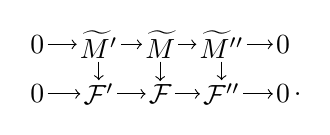
\begin{tikzpicture}[x=.78cm,y=.63cm,every node/.style={inner sep=1pt}]
\foreach \x/\word/\letter in {0/0/0,1/\widetilde M'/\mathcal F',2/\widetilde M/\mathcal F,3/\widetilde M''/\mathcal F'',4/0/0}
  {\node (a\x) at (\x,0) {$\word$}; \node (b\x) at (\x,-1) {$\letter$};}
\foreach \x/\z in {0/1,1/2,2/3,3/4}
  {\draw[->] (a\x) -- (a\z); \draw[->] (b\x) -- (b\z);}
\foreach \x in {1,2,3} \draw[->] (a\x) -- (b\x);
\node[anchor=west,inner sep=0pt] at (b4.east) {.};
\end{tikzpicture}
\]
The two outside arrows are isomorphisms, since $\mathcal F'$ and $\mathcal F''$ are quasi-coherent. So by the 5-lemma, the middle one is also, showing that $\mathcal F$ is quasi-coherent.
}
% Contents from body/page-129.tex.
\ChapterSheet{129}{115}{\Goto{sec-II-5}{5\quad Sheaves of Modules}}{%
\indent In the noetherian case, if $\mathcal F'$ and $\mathcal F''$ are coherent, then $M'$ and $M''$ are finitely generated, so $M$ is also finitely generated, and hence $\mathcal F$ is coherent.

\medskip
\noindent\hypertarget{result-II-5.8}{}\textbf{Proposition 5.8.} \emph{Let $f\colon X\to Y$ be a morphism of schemes.}
\par{\itshape\leftskip=12pt
\hypertarget{result-II-5.8a}{}(a) If $\mathcal G$ is a quasi-coherent sheaf of $\mathcal O_Y$-modules, then $f^*\mathcal G$ is a quasi-coherent sheaf of $\mathcal O_X$-modules.

\hypertarget{result-II-5.8b}{}(b) If $X$ and $Y$ are noetherian, and if $\mathcal G$ is coherent, then $f^*\mathcal G$ is coherent.

\hypertarget{result-II-5.8c}{}(c) Assume that either $X$ is noetherian, or $f$ is quasi-compact (Ex.~\Goto{ex-II-3.2}{3.2}) and separated. Then if $\mathcal F$ is a quasi-coherent sheaf of $\mathcal O_X$-modules, $f_*\mathcal F$ is a quasi-coherent sheaf of $\mathcal O_Y$-modules.\par}

\smallskip
\noindent\textsc{Proof.}\par
(a) The question is local on both $X$ and $Y$, so we can assume $X$ and $Y$ both affine. In this case the result follows from \Goto{result-II-5.5}{(5.5)} and \Goto{result-II-5.2e}{(5.2e)}.

(b) In the noetherian case, the same proof works for coherent sheaves.

(c) Here the question is local on $Y$ only, so we may assume that $Y$ is affine. Then $X$ is quasi-compact (under either hypothesis) so we can cover $X$ with a finite number of open affine subsets $U_i$. In the separated case, $U_i\cap U_j$ is again affine (Ex.~\Goto{ex-II-4.3}{4.3}). Call it $U_{ijk}$. In the noetherian case, $U_i\cap U_j$ is at least quasi-compact, so we can cover it with a finite number of open affine subsets $U_{ijk}$. Now for any open subset $V$ of $Y$, giving a section $s$ of $\mathcal F$ over $f^{-1}V$ is the same thing as giving a collection of sections $s_i$ of $\mathcal F$ over $(f^{-1}V)\cap U_i$ whose restrictions to the open subsets $f^{-1}(V)\cap U_{ijk}$ are all equal. This is just the sheaf property (\Goto{sec-II-1}{\S1}). Therefore, there is an exact sequence of sheaves on $Y$,
\[
0\to f_*\mathcal F\to\bigoplus_i f_*(\mathcal F|_{U_i})\to
\bigoplus_{i,j,k}f_*(\mathcal F|_{U_{ijk}}),
\]
where by abuse of notation we denote also by $f$ the induced morphisms $U_i\to Y$ and $U_{ijk}\to Y$. Now $f_*(\mathcal F|_{U_i})$ and $f_*(\mathcal F|_{U_{ijk}})$ are quasi-coherent by \Goto{result-II-5.2d}{(5.2d)}. Thus $f_*\mathcal F$ is quasi-coherent by \Goto{result-II-5.7}{(5.7)}.

\medskip
\noindent\hypertarget{result-II-5.8.1}{}\textbf{Caution 5.8.1.} If $X$ and $Y$ are noetherian, it is \emph{not} true in general that $f_*$ of a coherent sheaf is coherent (Ex.~\Goto{ex-II-5.5}{5.5}). However, it is true if $f$ is a finite morphism (Ex.~\Goto{ex-II-5.5}{5.5}) or a projective morphism \Goto{result-II-5.20}{(5.20)} or (III, \Goto{result-III-8.8}{8.8}), or more generally, a proper morphism: see Grothendieck \Goto{bib-EGA}{[EGA III, 3.2.1]}.

\medskip
As a first application of these concepts, we will discuss the sheaf of ideals of a closed subscheme.

\medskip
\noindent\textbf{Definition.} Let $Y$ be a closed subscheme of a scheme $X$, and let $i\colon Y\to X$ be the inclusion morphism. We define the \emph{ideal sheaf} of $Y$, denoted $\mathcal I_Y$, to be the kernel of the morphism $i^\#\colon\mathcal O_X\to i_*\mathcal O_Y$.
}
% Contents from body/page-130.tex.
\ChapterSheet{130}{116}{\Goto{p-74}{II\quad Schemes}}{%
\noindent\hypertarget{result-II-5.9}{}\textbf{Proposition 5.9.} \emph{Let $X$ be a scheme. For any closed subscheme $Y$ of $X$, the corresponding ideal sheaf $\mathcal I_Y$ is a quasi-coherent sheaf of ideals on $X$. If $X$ is noetherian, it is coherent. Conversely, any quasi-coherent sheaf of ideals on $X$ is the ideal sheaf of a uniquely determined closed subscheme of $X$.}

\smallskip
\noindent\textsc{Proof.} If $Y$ is a closed subscheme of $X$, then the inclusion morphism $i\colon Y\to X$ is quasi-compact (obvious) and separated \Goto{result-II-4.6}{(4.6)}, so by \Goto{result-II-5.8}{(5.8)}, $i_*\mathcal O_Y$ is quasi-coherent on $X$. Hence $\mathcal I_Y$, being the kernel of a morphism of quasi-coherent sheaves, is also quasi-coherent. If $X$ is noetherian, then for any open affine subset $U=\operatorname{Spec}A$ of $X$, the ring $A$ is noetherian, so the ideal $I=\Gamma(U,\mathcal I_Y|_U)$, is finitely generated, so $\mathcal I_Y$ is coherent.

Conversely, given a scheme $X$ and a quasi-coherent sheaf of ideals $\mathcal I$, let $Y$ be the support of the quotient sheaf $\mathcal O_X/\mathcal I$. Then $Y$ is a subspace of $X$, and $(Y,\mathcal O_X/\mathcal I)$ is the unique closed subscheme of $X$ with ideal sheaf $\mathcal I$. The unicity is clear, so we have only to check that $(Y,\mathcal O_X/\mathcal I)$ is a closed subscheme. This is a local question, so we may assume $X=\operatorname{Spec}A$ is affine. Since $\mathcal I$ is quasi-coherent, $\mathcal I=\widetilde{\mathfrak a}$ for some ideal $\mathfrak a\subseteq A$. Then $(Y,\mathcal O_X/\mathcal I)$ is just the closed subscheme of $X$ determined by the ideal $\mathfrak a$ \Goto{result-II-3.2.3}{(3.2.3)}.

\medskip
\noindent\hypertarget{result-II-5.10}{}\textbf{Corollary 5.10.} \emph{If $X=\operatorname{Spec}A$ is an affine scheme, there is a $1$-$1$ correspondence between ideals $\mathfrak a$ in $A$ and closed subschemes $Y$ of $X$, given by $\mathfrak a\mapsto$ image of $\operatorname{Spec}A/\mathfrak a$ in $X$ \Goto{result-II-3.2.3}{(3.2.3)}. In particular, every closed subscheme of an affine scheme is affine.}

\smallskip
\noindent\textsc{Proof.} By \Goto{result-II-5.5}{(5.5)} the quasi-coherent sheaves of ideals on $X$ are in $1$-$1$ correspondence with the ideals of $A$.

\medskip
Our next concern is to study quasi-coherent sheaves on the Proj of a graded ring. As in the case of Spec, there is a connection between modules over the ring and sheaves on the space, but it is more complicated.

\medskip
\noindent\textbf{Definition.} Let $S$ be a graded ring and let $M$ be a graded $S$-module. (See (I, \Goto{sec-I-7}{\S7}) for generalities on graded modules.) We define the \emph{sheaf associated} to $M$ on $\operatorname{Proj}S$, denoted by $\widetilde M$, as follows. For each $\mathfrak p\in\operatorname{Proj}S$, let $M_{(\mathfrak p)}$ be the group of elements of degree $0$ in the localization $T^{-1}M$, where $T$ is the multiplicative system of homogeneous elements of $S$ not in $\mathfrak p$ (cf. definition of Proj in \Goto{sec-II-2}{\S2}). For any open subset $U\subseteq\operatorname{Proj}S$ we define $\widetilde M(U)$ to be the set of functions $s$ from $U$ to $\coprod_{\mathfrak p\in U}M_{(\mathfrak p)}$ which are locally fractions. This means that for every $\mathfrak p\in U$, there is a neighborhood $V$ of $\mathfrak p$ in $U$, and homogeneous elements $m\in M$ and $f\in S$ of the same degree, such that for every $\mathfrak q\in V$, we have $f\notin\mathfrak q$, and $s(\mathfrak q)=m/f$ in $M_{(\mathfrak q)}$. We make $\widetilde M$ into a sheaf with the obvious restriction maps.

\medskip
\noindent\hypertarget{result-II-5.11}{}\textbf{Proposition 5.11.} \emph{Let $S$ be a graded ring, and $M$ a graded $S$-module. Let $X=\operatorname{Proj}S$.}
}
% Contents from body/page-131.tex.
\ChapterSheet{131}{117}{\Goto{sec-II-5}{5\quad Sheaves of Modules}}{%
{\itshape\leftskip=12pt
\hypertarget{result-II-5.11a}{}(a) For any $\mathfrak p\in X$, the stalk $(\widetilde M)_{\mathfrak p}=M_{(\mathfrak p)}$.

\hypertarget{result-II-5.11b}{}(b) For any homogeneous $f\in S_+$, we have $\widetilde M|_{D_+(f)}\cong(M_{(f)})^\sim$ via the isomorphism of $D_+(f)$ with $\operatorname{Spec}S_{(f)}$ (see \Goto{result-II-2.5b}{(2.5b)}), where $M_{(f)}$ denotes the group of elements of degree $0$ in the localized module $M_f$.

\hypertarget{result-II-5.11c}{}(c) $\widetilde M$ is a quasi-coherent $\mathcal O_X$-module. If $S$ is noetherian and $M$ is finitely generated, then $\widetilde M$ is coherent.\par}

\smallskip
\noindent\textsc{Proof.} For \Goto{result-II-5.11a}{(a)} and \Goto{result-II-5.11b}{(b)}, just repeat the proof of \Goto{result-II-2.5}{(2.5)}, with $M$ in place of $S$. Then \Goto{result-II-5.11c}{(c)} follows from \Goto{result-II-5.11b}{(b)}.

\medskip
\noindent\textbf{Definition.} Let $S$ be a graded ring, and let $X=\operatorname{Proj}S$. For any $n\in\mathbf Z$, we define the sheaf $\mathcal O_X(n)$ to be $S(n)^\sim$. We call $\mathcal O_X(1)$ the \emph{twisting sheaf} of Serre. For any sheaf of $\mathcal O_X$-modules, $\mathcal F$, we denote by $\mathcal F(n)$ the \emph{twisted sheaf} $\mathcal F\otimes_{\mathcal O_X}\mathcal O_X(n)$.

\medskip
\noindent\hypertarget{result-II-5.12}{}\textbf{Proposition 5.12.} \emph{Let $S$ be a graded ring and let $X=\operatorname{Proj}S$. Assume that $S$ is generated by $S_1$ as an $S_0$-algebra.}
\par{\itshape\leftskip=12pt
\hypertarget{result-II-5.12a}{}(a) The sheaf $\mathcal O_X(n)$ is an invertible sheaf on $X$.

\hypertarget{result-II-5.12b}{}(b) For any graded $S$-module $M$, $\widetilde M(n)\cong(M(n))^\sim$. In particular, $\mathcal O_X(n)\otimes\mathcal O_X(m)\cong\mathcal O_X(n+m)$.

\hypertarget{result-II-5.12c}{}(c) Let $T$ be another graded ring, generated by $T_1$ as a $T_0$-algebra, let $\varphi\colon S\to T$ be a homomorphism preserving degrees, and let $U\subseteq Y=\operatorname{Proj}T$ and $f\colon U\to X$ be the morphism determined by $\varphi$ (Ex.~\Goto{ex-II-2.14}{2.14}). Then $f^*(\mathcal O_X(n))\cong\mathcal O_Y(n)|_U$ and $f_*(\mathcal O_Y(n)|_U)\cong(f_*\mathcal O_U)(n)$.\par}

\smallskip
\noindent\textsc{Proof.}\par
(a) Recall that invertible means locally free of rank $1$. Let $f\in S_1$, and consider the restriction $\mathcal O_X(n)|_{D_+(f)}$. By the previous proposition this is isomorphic to $S(n)_{(f)}^\sim$ on $\operatorname{Spec}S_{(f)}$. We will show that this restriction is free of rank $1$. Indeed, $S(n)_{(f)}$ is a free $S_{(f)}$-module of rank $1$. For $S_{(f)}$ is the group of elements of degree $0$ in $S_f$, and $S(n)_{(f)}$ is the group of elements of degree $n$ in $S_f$. We obtain an isomorphism of one to the other by sending $s$ to $f^ns$. This makes sense, for any $n\in\mathbf Z$, because $f$ is invertible in $S_f$. Now since $S$ is generated by $S_1$ as an $S_0$-algebra, $X$ is covered by the open sets $D_+(f)$ for $f\in S_1$. Hence $\mathcal O(n)$ is invertible.

(b) This follows from the fact that $(M\otimes_S N)^\sim\cong\widetilde M\otimes_{\mathcal O_X}\widetilde N$ for any two graded $S$-modules $M$ and $N$, when $S$ is generated by $S_1$. Indeed, for any $f\in S_1$ we have $(M\otimes_S N)_{(f)}=M_{(f)}\otimes_{S_{(f)}}N_{(f)}$.

(c) More generally, for any graded $S$-module $M$, $f^*(\widetilde M)\cong(M\otimes_S T)^\sim|_U$ and for any graded $T$-module $N$, $f_*(\widetilde N|_U)\cong({}_SN)^\sim$. Furthermore, the sheaf $\widetilde T$ on $X$ is just $f_*(\mathcal O_U)$. The proofs are straightforward (cf. \Goto{result-II-5.2}{(5.2)} for the affine case).

\medskip
The twisting operation allows us to define a graded $S$-module associated to any sheaf of modules on $X=\operatorname{Proj}S$.
}
% Contents from body/page-132.tex.
\ChapterSheet{132}{118}{\Goto{p-74}{II\quad Schemes}}{%
\noindent\textbf{Definition.} Let $S$ be a graded ring, let $X=\operatorname{Proj}S$, and let $\mathcal F$ be a sheaf of $\mathcal O_X$-modules. We define the \emph{graded $S$-module associated} to $\mathcal F$ as a group, to be $\Gamma_*(\mathcal F)=\bigoplus_{n\in\mathbf Z}\Gamma(X,\mathcal F(n))$. We give it a structure of graded $S$-module as follows. If $s\in S_d$, then $s$ determines in a natural way a global section $s\in\Gamma(X,\mathcal O_X(d))$. Then for any $t\in\Gamma(X,\mathcal F(n))$ we define the product $s\cdot t$ in $\Gamma(X,\mathcal F(n+d))$ by taking the tensor product $s\otimes t$ and using the natural map
\EditionText{$\mathcal F(n)\otimes\mathcal O_X(d)\to\mathcal F(n+d)$}.

\medskip
\noindent\hypertarget{result-II-5.13}{}\textbf{Proposition 5.13.} \emph{Let $A$ be a ring, let $S=A[x_0,\ldots,x_r]$, $r\geq1$, and let $X=\operatorname{Proj}S$. (This is just projective $r$-space over $A$.) Then $\Gamma_*(\mathcal O_X)\cong S$.}

\smallskip
\noindent\textsc{Proof.} We cover $X$ with the open sets $D_+(x_i)$. Then to give a section $t\in\Gamma(X,\mathcal O_X(n))$ is the same as giving sections $t_i\in\mathcal O_X(n)(D_+(x_i))$ for each $i$, which agree on the intersections $D_+(x_ix_j)$. Now $t_i$ is just a homogeneous element of degree $n$ in the localization $S_{x_i}$, and its restriction to $D_+(x_ix_j)$ is just the image of that element in $S_{x_ix_j}$. Summing over all $n$, we see that $\Gamma_*(\mathcal O_X)$ can be identified with the set of $(r+1)$-tuples $(t_0,\ldots,t_r)$ where for each $i$, $t_i\in S_{x_i}$, and for each $i,j$, the images of $t_i$ and $t_j$ in $S_{x_ix_j}$ are the same.

Now the $x_i$ are not zero divisors in $S$, so the localization maps $S\to S_{x_i}$ and $S_{x_i}\to S_{x_ix_j}$ are all injective, and these rings are all subrings of $S'=S_{x_0\cdots x_r}$. Hence $\Gamma_*(\mathcal O_X)$ is the intersection $\bigcap S_{x_i}$ taken inside $S'$. Now any homogeneous element of $S'$ can be written uniquely as a product $x_0^{i_0}\cdots x_r^{i_r}f(x_0,\ldots,x_r)$, where the $i_j\in\mathbf Z$, and $f$ is a homogeneous polynomial not divisible by any $x_i$. This element will be in $S_{x_i}$ if and only if $i_j\geq0$ for $j\ne i$. It follows that the intersection of all the $S_{x_i}$ (in fact the intersection of any two of them) is exactly $S$.

\medskip
\noindent\hypertarget{result-II-5.13.1}{}\textbf{Caution 5.13.1.} If $S$ is a graded ring which is not a polynomial ring, then it is not true in general that $\Gamma_*(\mathcal O_X)=S$ (Ex.~\Goto{ex-II-5.14}{5.14}).

\medskip
\noindent\hypertarget{result-II-5.14}{}\textbf{Lemma 5.14.} \emph{Let $X$ be a scheme, let $\mathcal L$ be an invertible sheaf on $X$, let $f\in\Gamma(X,\mathcal L)$, let $X_f$ be the open set of points $x\in X$ where $f_x\notin\mathfrak m_x\mathcal L_x$, and let $\mathcal F$ be a quasi-coherent sheaf on $X$.}
\par{\itshape\leftskip=12pt
\hypertarget{result-II-5.14a}{}(a) Suppose that $X$ is quasi-compact, and let $s\in\Gamma(X,\mathcal F)$ be a global section of $\mathcal F$ whose restriction to $X_f$ is $0$. Then for some $n>0$, we have $f^ns=0$, where $f^ns$ is considered as a global section of $\mathcal F\otimes\mathcal L^{\otimes n}$.

\hypertarget{result-II-5.14b}{}(b) Suppose furthermore that $X$ has a finite covering by open affine subsets $U_i$, such that $\mathcal L|_{U_i}$ is free for each $i$, and such that $U_i\cap U_j$ is quasi-compact for each $i,j$. Given a section $t\in\Gamma(X_f,\mathcal F)$, then for some $n>0$, the section $f^nt\in\Gamma(X_f,\mathcal F\otimes\mathcal L^{\otimes n})$ extends to a global section of $\mathcal F\otimes\mathcal L^{\otimes n}$.\par}

\smallskip
\noindent\textsc{Proof.} This lemma is a direct generalization of \Goto{result-II-5.3}{(5.3)}, with an extra twist due to the presence of the invertible sheaf $\mathcal L$. It also generalizes (Ex.~\Goto{ex-II-2.16}{2.16}). To prove \Goto{result-II-5.14a}{(a)}, we first cover $X$ with a finite number (possible since $X$ is quasi-compact) of open affines $U=\operatorname{Spec}A$ such that $\mathcal L|_U$ is free. Let $\psi\colon\mathcal L|_U\cong\mathcal O_U$ be an isomorphism expressing the freeness of $\mathcal L|_U$. Since $\mathcal F$ is quasi-coherent,
}
% Contents from body/page-133.tex.
\ChapterSheet{133}{119}{\Goto{sec-II-5}{5\quad Sheaves of Modules}}{%
by \Goto{result-II-5.4}{(5.4)} there is an $A$-module $M$ with $\mathcal F|_U\cong\widetilde M$. Our section $s\in\Gamma(X,\mathcal F)$ restricts to give an element $s\in M$. On the other hand, our section $f\in\Gamma(X,\mathcal L)$ restricts to give a section of $\mathcal L|_U$, which in turn gives rise to an element $g=\psi(f)\in A$. Clearly $X_f\cap U=D(g)$. Now $s|_{X_f}$ is zero, so $g^ns=0$ in $M$ for some $n>0$, just as in the proof of \Goto{result-II-5.3}{(5.3)}. Using the isomorphism
\[
\mathrm{id}\times\psi^{\otimes n}\colon(\mathcal F\otimes\mathcal L^{\otimes n})|_U\cong\mathcal F|_U,
\]
we conclude that $f^ns\in\Gamma(U,\mathcal F\otimes\mathcal L^{\otimes n})$ is zero. This statement is intrinsic (i.e., independent of $\psi$). So we can do this for each open set of the covering, pick one $n$ large enough to work for all the sets of the covering, and we find $f^ns=0$ on $X$.

To prove \Goto{result-II-5.14b}{(b)}, we proceed as in the proof of \Goto{result-II-5.3}{(5.3)}, keeping track of the twist due to $\mathcal L$ as above. The hypothesis $U_i\cap U_j$ quasi-compact is used to be able to apply part \Goto{result-II-5.14a}{(a)} there.

\medskip
\noindent\hypertarget{result-II-5.14.1}{}\textbf{Remark 5.14.1.} The hypotheses on $X$ made in the statements \Goto{result-II-5.14a}{(a)} and \Goto{result-II-5.14b}{(b)} above are satisfied either if $X$ is noetherian (in which case every open set is quasi-compact) or if $X$ is quasi-compact and separated (in which case the intersection of two open affine subsets is again affine, hence quasi-compact).

\medskip
\noindent\hypertarget{result-II-5.15}{}\textbf{Proposition 5.15.} \emph{Let $S$ be a graded ring, which is finitely generated by $S_1$ as an $S_0$-algebra. Let $X=\operatorname{Proj}S$, and let $\mathcal F$ be a quasi-coherent sheaf on $X$. Then there is a natural isomorphism $\beta\colon\Gamma_*(\mathcal F)^\sim\to\mathcal F$.}

\smallskip
\noindent\textsc{Proof.} First let us define the morphism $\beta$ for any $\mathcal O_X$-module $\mathcal F$. Let $f\in S_1$. Since $\Gamma_*(\mathcal F)^\sim$ is quasi-coherent in any case, to define $\beta$, it is enough to give the image of a section of $\Gamma_*(\mathcal F)^\sim$ over $D_+(f)$ (see Ex.~\Goto{ex-II-5.3}{5.3}). Such a section is represented by a fraction $m/f^d$, where $m\in\Gamma(X,\mathcal F(d))$, for some $d\geq0$. We can think of $f^{-d}$ as a section of $\mathcal O_X(-d)$, defined over $D_+(f)$. Taking their tensor product, we obtain $m\otimes f^{-d}$ as a section of $\mathcal F$ over $D_+(f)$. This defines $\beta$.

Now let $\mathcal F$ be quasi-coherent. To show that $\beta$ is an isomorphism we have to identify the module $\Gamma_*(\mathcal F)_{(f)}$ with the sections of $\mathcal F$ over $D_+(f)$. We apply \Goto{result-II-5.14}{(5.14)}, considering $f$ as a global section of the invertible sheaf $\mathcal L=\mathcal O(1)$. Since we have assumed that $S$ is finitely generated by $S_1$ as an $S_0$-algebra, we can find finitely many elements $f_0,\ldots,f_r\in S_1$ such that $X$ is covered by the open affine subsets $D_+(f_i)$. The intersections $D_+(f_i)\cap D_+(f_j)$ are also affine, and $\mathcal L|_{D_+(f_i)}$ is free for each $i$, so the hypotheses of \Goto{result-II-5.14}{(5.14)} are satisfied. The conclusion of \Goto{result-II-5.14}{(5.14)} tells us that $\mathcal F(D_+(f))\cong\Gamma_*(\mathcal F)_{(f)}$, which is just what we wanted.

\medskip
\noindent\hypertarget{result-II-5.16}{}\textbf{Corollary 5.16.} \emph{Let $A$ be a ring.}
\par{\itshape\leftskip=12pt
\hypertarget{result-II-5.16a}{}(a) If $Y$ is a closed subscheme of $\Proj_A^r$, then there is a homogeneous ideal $I\subseteq S=A[x_0,\ldots,x_r]$ such that $Y$ is the closed subscheme determined by $I$ (Ex.~\Goto{ex-II-3.12}{3.12}).\par}
}
% Contents from body/page-134.tex.
\ChapterSheet[10.9]{134}{120}{\Goto{p-74}{II\quad Schemes}}{%
{\itshape\leftskip=12pt
\hypertarget{result-II-5.16b}{}(b) A scheme $Y$ over $\operatorname{Spec}A$ is projective if and only if it is isomorphic to $\operatorname{Proj}S$ for some graded ring $S$, where $S_0=A$, and $S$ is finitely generated by $S_1$ as an $S_0$-algebra.\par}

\smallskip
\noindent\textsc{Proof.}\par
(a) Let $\mathcal I_Y$ be the ideal sheaf of $Y$ on $X=\Proj_A^r$. Now $\mathcal I_Y$ is a subsheaf of $\mathcal O_X$; the twisting functor is exact; the global section functor $\Gamma$ is left exact;
\EditionText{write $\Gamma_{\geq0}(\mathcal G)=\bigoplus_{n\geq0}\Gamma(X,\mathcal G(n))$. Then $\Gamma_{\geq0}(\mathcal I_Y)$ is a submodule of $\Gamma_{\geq0}(\mathcal O_X)$. The latter is $S$, by \Goto{result-II-5.13}{(5.13)} for $r\geq1$ and by the trivialization by $x_0$ for $r=0$. Hence $\Gamma_{\geq0}(\mathcal I_Y)$ is a homogeneous ideal of $S$, which we will call $I$.}
Now $I$ determines a closed subscheme of $X$ (Ex.~\Goto{ex-II-3.12}{3.12}), whose sheaf of ideals will be $\widetilde I$. Since $\mathcal I_Y$ is quasi-coherent by \Goto{result-II-5.9}{(5.9)}, we have $\mathcal I_Y\cong\widetilde I$ by \Goto{result-II-5.15}{(5.15)}%
\EditionText{ (discarding the negative degrees does not change the associated sheaf: on $D_+(x_i)$ multiply the numerator and denominator of a homogeneous fraction by a suitable power of $x_i$)}%
, and hence $Y$ is the subscheme determined by $I$. In fact, \EditionText{$\Gamma_{\geq0}(\mathcal I_Y)$} is the largest ideal in $S$ defining $Y$ (Ex.~\Goto{ex-II-5.10}{5.10}).

(b) Recall that by definition $Y$ is projective over $\operatorname{Spec}A$ if it is isomorphic to a closed subscheme of $\Proj_A^r$ for some $r$ (\Goto{sec-II-4}{\S4}). By part \Goto{result-II-5.16a}{(a)}, any such $Y$ is isomorphic to $\operatorname{Proj}S/I$, and we can take $I$ to be contained in $S_+=\bigoplus_{d>0}S_d$ (Ex.~\Goto{ex-II-3.12}{3.12}), so that $(S/I)_0=A$. Conversely, any such graded ring $S$ is a quotient of a polynomial ring, so $\operatorname{Proj}S$ is projective.

\medskip
\noindent\textbf{Definition.} For any scheme $Y$, we define the \emph{twisting sheaf} $\mathcal O(1)$ on $\Proj_Y^r$ to be $g^*(\mathcal O(1))$, where $g\colon\Proj_Y^r\to\Proj_{\mathbf Z}^r$ is the natural map (recall that $\Proj_Y^r$ was defined as $\Proj_{\mathbf Z}^r\times_{\mathbf Z}Y$).

Note that if $Y=\operatorname{Spec}A$, this is the same as the $\mathcal O(1)$ already defined on $\Proj_A^r=\operatorname{Proj}A[x_0,\ldots,x_r]$, by \Goto{result-II-5.12c}{(5.12c)}.

\medskip
\noindent\textbf{Definition.} If $X$ is any scheme over $Y$, an invertible sheaf $\mathcal L$ on $X$ is \emph{very ample relative to $Y$}, if there is an immersion $i\colon X\to\Proj_Y^r$ for some $r$, such that $i^*(\mathcal O(1))\cong\mathcal L$. We say that a morphism $i\colon X\to Z$ is an \emph{immersion} if it gives an isomorphism of $X$ with an open subscheme of a closed subscheme of $Z$. (This definition of very ample differs slightly from the one in Grothendieck \Goto{bib-EGA}{[EGA II, 4.4.2]}.)

\medskip
\noindent\hypertarget{result-II-5.16.1}{}\textbf{Remark 5.16.1.} Let $Y$ be a noetherian scheme. Then a scheme $X$ over $Y$ is projective if and only if it is proper, and there exists a very ample sheaf on $X$ relative to $Y$. Indeed, if $X$ is projective over $Y$, then $X$ is proper by \Goto{result-II-4.9}{(4.9)}. On the other hand, there is a closed immersion $i\colon X\to\Proj_Y^r$ for some $r$, so $i^*\mathcal O(1)$ is a very ample invertible sheaf on $X$. Conversely, if $X$ is proper over $Y$, and $\mathcal L$ is a very ample invertible sheaf, then $\mathcal L\cong i^*(\mathcal O(1))$ for some immersion $i\colon X\to\Proj_Y^r$. But by (Ex.~\Goto{ex-II-4.4}{4.4}) the image of $X$ is closed, so in fact $i$ is a closed immersion, so $X$ is projective over $Y$.

Note however that there may be several nonisomorphic very ample sheaves on a projective scheme $X$ over $Y$. The sheaf $\mathcal L$ depends on the embedding of $X$ into $\Proj_Y^r$ (Ex.~\Goto{ex-II-5.12}{5.12}). If $Y=\operatorname{Spec}A$, and if $X=\operatorname{Proj}S$, where $S$ is a graded ring as in \Goto{result-II-5.16b}{(5.16b)}, then the sheaf $\mathcal O(1)$ on $X$ defined earlier is a very ample sheaf on $X$. However, there may be nonisomorphic graded rings having the same Proj and the same very ample sheaf $\mathcal O(1)$ (Ex.~\Goto{ex-II-2.14}{2.14}).
}
% Contents from body/page-135.tex.
\ChapterSheet{135}{121}{\Goto{sec-II-5}{5\quad Sheaves of Modules}}{%
\indent We end this section with some special results about sheaves on a projective scheme over a noetherian ring.

\medskip
\noindent\textbf{Definition.} Let $X$ be a scheme, and let $\mathcal F$ be a sheaf of $\mathcal O_X$-modules. We say that $\mathcal F$ is \emph{generated by global sections} if there is a family of global sections $\{s_i\}_{i\in I}$, $s_i\in\Gamma(X,\mathcal F)$, such that for each $x\in X$, the images of $s_i$ in the stalk $\mathcal F_x$ generate that stalk as an $\mathcal O_x$-module.

Note that $\mathcal F$ is generated by global sections if and only if $\mathcal F$ can be written as a quotient of a free sheaf. Indeed, the generating sections $\{s_i\}_{i\in I}$ define a surjective morphism of sheaves $\bigoplus_{i\in I}\mathcal O_X\to\mathcal F$, and conversely.

\medskip
\noindent\hypertarget{result-II-5.16.2}{}\textbf{Example 5.16.2.} Any quasi-coherent sheaf on an affine scheme is generated by global sections. Indeed, if $\mathcal F=\widetilde M$ on $\operatorname{Spec}A$, any set of generators for $M$ as an $A$-module will do.

\medskip
\noindent\hypertarget{result-II-5.16.3}{}\textbf{Example 5.16.3.} Let $X=\operatorname{Proj}S$, where $S$ is a graded ring which is generated by $S_1$ as an $S_0$-algebra. Then the elements of $S_1$ give global sections of $\mathcal O_X(1)$ which generate it.

\medskip
\noindent\hypertarget{result-II-5.17}{}\textbf{Theorem 5.17} (Serre). \emph{Let $X$ be a projective scheme over a noetherian ring $A$, let $\mathcal O(1)$ be a very ample invertible sheaf on $X$, and let $\mathcal F$ be a coherent $\mathcal O_X$-module. Then there is an integer $n_0$ such that for all $n\geq n_0$, the sheaf $\mathcal F(n)$ can be generated by a finite number of global sections.}

\smallskip
\noindent\textsc{Proof.} Let $i\colon X\to\Proj_A^r$ be a closed immersion of $X$ into a projective space over $A$, such that $i^*(\mathcal O(1))=\mathcal O_X(1)$. Then $i_*\mathcal F$ is coherent on $\Proj_A^r$ (Ex.~\Goto{ex-II-5.5}{5.5}), and $i_*(\mathcal F(n))=(i_*\mathcal F)(n)$ \Goto{result-II-5.12}{(5.12)} or (Ex.~\Goto{ex-II-5.1}{5.1d}), and $\mathcal F(n)$ is generated by global sections if and only if $i_*(\mathcal F(n))$ is (in fact, their global sections are the same), so we reduce to the case $X=\Proj_A^r=\operatorname{Proj}A[x_0,\ldots,x_r]$.

Now cover $X$ with the open sets $D_+(x_i)$, $i=0,\ldots,r$. Since $\mathcal F$ is coherent, for each $i$ there is a finitely generated module $M_i$ over $B_i=A[x_0/x_i,\ldots,\EditionText{x_r}/x_i]$ such that $\mathcal F|_{D_+(x_i)}\cong\widetilde M_i$. For each $i$, take a finite number of elements $s_{ij}\in M_i$ which generate this module. By \Goto{result-II-5.14}{(5.14)} there is an integer $n$ such that $x_i^ns_{ij}$ extends to a global section $t_{ij}$ of $\mathcal F(n)$. As usual, we take one $n$ to work for all $i,j$. Now $\mathcal F(n)$ corresponds to a $B_i$-module $M_i'$ on $D_+(x_i)$, and the map $x_i^n\colon\mathcal F\to\mathcal F(n)$ induces an \emph{isomorphism} of $M_i$ to $M_i'$. So the sections $x_i^ns_{ij}$ generate $M_i'$, and hence the global sections $t_{ij}\in\Gamma(X,\mathcal F(n))$ generate the sheaf $\mathcal F(n)$ everywhere.

\medskip
\noindent\hypertarget{result-II-5.18}{}\textbf{Corollary 5.18.} \emph{Let $X$ be projective over a noetherian ring $A$. Then any coherent sheaf $\mathcal F$ on $X$ can be written as a quotient of a sheaf $\mathcal E$, where $\mathcal E$ is a finite direct sum of twisted structure sheaves $\mathcal O(n_i)$ for various integers $n_i$.}
}
% Contents from body/page-136.tex.
\ChapterSheet{136}{122}{\Goto{p-74}{II\quad Schemes}}{%
\noindent\textsc{Proof.} Let $\mathcal F(n)$ be generated by a finite number of global sections. Then we have a surjection $\bigoplus_{i=1}^N\mathcal O_X\to\mathcal F(n)\to0$. Tensoring with $\mathcal O_X(-n)$ we obtain a surjection $\bigoplus_{i=1}^N\mathcal O_X(-n)\to\mathcal F\to0$ as required.

\medskip
\noindent\hypertarget{result-II-5.19}{}\textbf{Theorem 5.19.} \emph{Let $k$ be a field, let $A$ be a finitely generated $k$-algebra, let $X$ be a projective scheme over $A$, and let $\mathcal F$ be a coherent $\mathcal O_X$-module. Then $\Gamma(X,\mathcal F)$ is a finitely generated $A$-module. In particular, if $A=k$, $\Gamma(X,\mathcal F)$ is a finite-dimensional $k$-vector space.}

\smallskip
\noindent\textsc{Proof.} First we write $X=\operatorname{Proj}S$, where $S$ is a graded ring with $S_0=A$ which is finitely generated by $S_1$ as an $S_0$-algebra \Goto{result-II-5.16b}{(5.16b)}. Let $M$ be the graded $S$-module $\Gamma_*(\mathcal F)$. Then by \Goto{result-II-5.15}{(5.15)} we have $\widetilde M\cong\mathcal F$. On the other hand, by \Goto{result-II-5.17}{(5.17)}, for $n$ sufficiently large, $\mathcal F(n)$ is generated by a finite number of global sections in $\Gamma(X,\mathcal F(n))$. Let $M'$ be the submodule of $M$ generated by these sections. Then $M'$ is a finitely generated $S$-module. Furthermore, the inclusion $M'\hookrightarrow M$ induces an inclusion of sheaves $\widetilde M'\hookrightarrow\widetilde M=\mathcal F$. Twisting by $n$ we have an inclusion $\widetilde M'(n)\hookrightarrow\mathcal F(n)$ which is actually an isomorphism, because $\mathcal F(n)$ is generated by global sections in $M'$. Twisting by $-n$ we find that $\widetilde M'\cong\mathcal F$. Thus $\mathcal F$ is the sheaf associated to a finitely generated $S$-module, and so we have reduced to showing that if $M$ is a finitely generated $S$-module, then $\Gamma(X,\widetilde M)$ is a finitely generated $A$-module.

Now by (I, \Goto{result-I-7.4}{7.4}), there is a finite filtration
\[
0=M^0\subseteq M^1\subseteq\cdots\subseteq M^r=M
\]
of $M$ by graded submodules, where for each $i$, $M^i/M^{i-1}\cong(S/\mathfrak p_i)(n_i)$ for some homogeneous prime ideal $\mathfrak p_i\subseteq S$, and some integer $n_i$. This filtration gives a filtration of $\widetilde M$, and the short exact sequences
\[
0\to\widetilde M^{i-1}\to\widetilde M^i\to\widetilde M^i/\widetilde M^{i-1}\to0
\]
give rise to left-exact sequences
\[
0\to\Gamma(X,\widetilde M^{i-1})\to\Gamma(X,\widetilde M^i)\to\Gamma(X,\widetilde M^i/\widetilde M^{i-1}).
\]
Thus to show that $\Gamma(X,\widetilde M)$ is finitely generated over $A$, it will be sufficient to show that $\Gamma(X,(S/\mathfrak p)^\sim(n))$ is finitely generated, for each $\mathfrak p$ and $n$. Thus we have reduced to the following special case: Let $S$ be a graded integral domain, finitely generated by $S_1$ as an $S_0$-algebra, where $S_0=A$ is a finitely generated integral domain over $k$. Then $\Gamma(X,\mathcal O_X(n))$ is a finitely generated $A$-module, for any $n\in\mathbf Z$.

\EditionText{If $S_1=0$, then $X=\varnothing$ and the required module is zero. Otherwise, let $x_0,\ldots,x_r\in S_1$ be a set of nonzero generators of $S_1$ as an $A$-module.} Since $S$ is an integral domain, multiplication by $x_0$ gives an injection $S(n)\to S(n+1)$ for any $n$. Hence there is an injection $\Gamma(X,\mathcal O_X(n))\to\Gamma(X,\mathcal O_X(n+1))$ for any $n$. Thus it is sufficient to prove $\Gamma(X,\mathcal O_X(n))$ finitely generated for all sufficiently large $n$, say $n\geq0$.

Let $S'=\bigoplus_{n\geq0}\Gamma(X,\mathcal O_X(n))$. Then $S'$ is a ring, containing $S$, and contained in the intersection $\bigcap S_{x_i}$ of the localizations of $S$ at the elements $x_0,\ldots,x_r$.
}
% Contents from body/page-137.tex.
\ChapterSheet{137}{123}{\Goto{sec-II-5}{5\quad Sheaves of Modules}}{%
\noindent(Use the same argument as in the proof of (\Goto{result-II-5.13}{5.13}).) We will show that $S'$ is integral over $S$.

Let $s'\in S'$ be homogeneous of degree $d\ge 0$. Since $s'\in S_{x_i}$ for each $i$, we can find an integer $n$ such that $x_i^ns'\in S$. Choose one $n$ that works for all $i$. Since the $x_i$ generate $S_1$, the monomials in the $x_i$ of degree $m$ generate $S_m$ for any $m$. So by taking a larger $n$, we may assume that $ys'\in S$ for all $y\in S_n$. In fact, since $s'$ has \EditionText{nonnegative} degree, we can say that for any $y\in S_{\ge n}=\bigoplus_{e\ge n}S_e$, $ys'\in S_{\ge n}$. Now it follows inductively, for any $q\ge 1$ that $y\cdot(s')^q\in S_{\ge n}$ for any $y\in S_{\ge n}$. Take for example $y=x_0^n$. Then for every $q\ge 1$ we have $(s')^q\in(1/x_0^n)S$. This is a finitely generated sub-$S$-module of the quotient field of $S'$. It follows by a well-known criterion for integral dependence (Atiyah--Macdonald \Goto{legacy-b-am}{[1, p.~59]}), that $s'$ is integral over $S$. Thus $S'$ is contained in the integral closure of $S$ in its quotient field.

To complete the proof, we apply the theorem of finiteness of integral closure (I, \Goto{result-I-3.9A}{3.9A}). Since $S$ is a finitely generated $k$-algebra, $S'$ will be a finitely generated $S$-module. It follows that for every $n$, $S'_n$ is a finitely generated $S_0$-module, which is what we wanted to prove. In fact, our proof shows that $S'_n=S_n$ for all sufficiently large $n$ (Ex.~\Goto{ex-II-5.9}{5.9}) and (Ex.~\Goto{ex-II-5.14}{5.14}).

\medskip
\noindent\hypertarget{result-II-5.19.1}{}\textbf{Remark 5.19.1.} This proof is a generalization of the proof of (I, \Goto{result-I-3.4}{3.4a}). We will give another proof of this theorem later, using cohomology (III, \Goto{result-III-5.2.1}{5.2.1}).

\medskip
\noindent\hypertarget{result-II-5.19.2}{}\textbf{Remark 5.19.2.} The hypothesis \textquotedblleft{}$A$ is a finitely generated $k$-algebra\textquotedblright{} is used only to be able to apply (I, \Goto{result-I-3.9A}{3.9A}). Thus it would be sufficient to assume only that $A$ is a \textquotedblleft{}Nagata ring\textquotedblright{} in the sense of Matsumura \Goto{bib-479-17}{[2, p.~231]}---see also \Goto{bib-479-17}{[loc.\ cit., Th.~72, p.~240]}.

\medskip
\noindent\hypertarget{result-II-5.20}{}\textbf{Corollary 5.20.} \emph{Let $f\colon X\to Y$ be a projective morphism of schemes of finite type over a field $k$. Let $\mathcal F$ be a coherent sheaf on $X$. Then $f_*\mathcal F$ is coherent on $Y$.}

\smallskip
\noindent\textsc{Proof.} The question is local on $Y$, so we may assume $Y=\operatorname{Spec} A$, where $A$ is a finitely generated $k$-algebra. Then in any case, $f_*\mathcal F$ is quasi-coherent (\Goto{result-II-5.8}{5.8c}), so $f_*\mathcal F=\Gamma(Y,f_*\mathcal F)^\sim=\Gamma(X,\mathcal F)^\sim$. But $\Gamma(X,\mathcal F)$ is a finitely generated $A$-module by the theorem, so $f_*\mathcal F$ is coherent. See (III, \Goto{result-III-8.8}{8.8}) for another proof and generalization.

\medskip
\noindent\textsc{Exercises}

\smallskip
\noindent\hypertarget{ex-II-5.1}{}\textbf{5.1.} Let $(X,\mathcal O_X)$ be a ringed space, and let $\mathcal E$ be a locally free $\mathcal O_X$-module of finite rank. We define the \emph{dual} of $\mathcal E$, denoted $\check{\mathcal E}$, to be the sheaf $\mathcal Hom_{\mathcal O_X}(\mathcal E,\mathcal O_X)$.

\noindent\hspace*{1.7em}(a) Show that $(\check{\mathcal E})^\vee\cong\mathcal E$.

\noindent\hspace*{1.7em}(b) For any $\mathcal O_X$-module $\mathcal F$, $\mathcal Hom_{\mathcal O_X}(\mathcal E,\mathcal F)\cong\check{\mathcal E}\otimes_{\mathcal O_X}\mathcal F$.

\noindent\hspace*{1.7em}(c) For any $\mathcal O_X$-modules $\mathcal F,\mathcal G$,
\[
\operatorname{Hom}_{\mathcal O_X}(\mathcal E\otimes\mathcal F,\mathcal G)
\cong\operatorname{Hom}_{\mathcal O_X}(\mathcal F,\mathcal Hom_{\mathcal O_X}(\mathcal E,\mathcal G)).
\]}
% Contents from body/page-138.tex.
\ChapterSheet[10.5]{138}{124}{\Goto{p-74}{II\quad Schemes}}{%
\fontsize{9.5}{10.5}\selectfont%
\setlength{\parskip}{0pt}%
\setlength{\smallskipamount}{2pt}%
\noindent\hangindent=3em\hspace*{1.7em}(d) (\emph{Projection Formula}). If $f\colon(X,\mathcal O_X)\to(Y,\mathcal O_Y)$ is a morphism of ringed spaces, if $\mathcal F$ is an $\mathcal O_X$-module, and if $\mathcal E$ is a locally free $\mathcal O_Y$-module of finite rank, then there is a natural isomorphism $f_*(\mathcal F\otimes_{\mathcal O_X}f^*\mathcal E)\cong f_*(\mathcal F)\otimes_{\mathcal O_Y}\mathcal E$.

\smallskip
\noindent\hypertarget{ex-II-5.2}{}\textbf{5.2.} Let $R$ be a discrete valuation ring with quotient field $K$, and let $X=\operatorname{Spec} R$.

\noindent\hangindent=3em\hspace*{1.7em}(a) To give an $\mathcal O_X$-module is equivalent to giving an $R$-module $M$, a $K$-vector space $L$, and a homomorphism $\rho\colon M\otimes_R K\to L$.

\noindent\hangindent=3em\hspace*{1.7em}(b) That $\mathcal O_X$-module is quasi-coherent if and only if $\rho$ is an isomorphism.

\smallskip
\noindent\hypertarget{ex-II-5.3}{}\textbf{5.3.} Let $X=\operatorname{Spec} A$ be an affine scheme. Show that the functors $\sim$ and $\Gamma$ are adjoint, in the following sense: for any $A$-module $M$, and for any sheaf of $\mathcal O_X$-modules $\mathcal F$, there is a natural isomorphism
\[
\operatorname{Hom}_A(M,\Gamma(X,\mathcal F))
\cong\operatorname{Hom}_{\mathcal O_X}(\widetilde M,\mathcal F).
\]

\smallskip
\noindent\hypertarget{ex-II-5.4}{}\textbf{5.4.} Show that a sheaf of $\mathcal O_X$-modules $\mathcal F$ on a scheme $X$ is quasi-coherent if and only if every point of $X$ has a neighborhood $U$, such that $\mathcal F|_U$ is isomorphic to a cokernel of a morphism of free sheaves on~$U$. If $X$ is noetherian, then $\mathcal F$ is coherent if and only if it is locally a cokernel of a morphism of free sheaves of finite rank. (These properties were originally the definition of quasi-coherent and coherent sheaves.)

\smallskip
\noindent\hypertarget{ex-II-5.5}{}\textbf{5.5.} Let $f\colon X\to Y$ be a morphism of schemes.

\noindent\hangindent=3em\hspace*{1.7em}(a) Show by example that if $\mathcal F$ is coherent on $X$, then $f_*\mathcal F$ need not be coherent on $Y$, even if $X$ and $Y$ are varieties over a field $k$.

\noindent\hangindent=3em\hspace*{1.7em}(b) Show that a closed immersion is a finite morphism (\Goto{sec-II-3}{\S3}).

\noindent\hangindent=3em\hspace*{1.7em}(c) If $f$ is a finite morphism of noetherian schemes, and if $\mathcal F$ is coherent on $X$, then $f_*\mathcal F$ is coherent on $Y$.

\smallskip
\noindent\hypertarget{ex-II-5.6}{}\textbf{5.6.} \emph{Support.} Recall the notions of support of a section of a sheaf, support of a sheaf, and subsheaf with supports from (Ex.~\Goto{ex-II-1.14}{1.14}) and (Ex.~\Goto{ex-II-1.20}{1.20}).

\noindent\hangindent=3em\hspace*{1.7em}(a) Let $A$ be a ring, let $M$ be an $A$-module, let $X=\operatorname{Spec} A$, and let $\mathcal F=\widetilde M$. For any $m\in M=\Gamma(X,\mathcal F)$, show that $\operatorname{Supp} m=V(\operatorname{Ann}m)$, where $\operatorname{Ann}m$ is the \emph{annihilator} of $m=\{a\in A\mid am=0\}$.

\noindent\hangindent=3em\hspace*{1.7em}(b) Now suppose that $A$ is noetherian, and $M$ finitely generated. Show that $\operatorname{Supp}\mathcal F=V(\operatorname{Ann} M)$.

\noindent\hangindent=3em\hspace*{1.7em}(c) The support of a coherent sheaf on a noetherian scheme is closed.

\noindent\hangindent=3em\hspace*{1.7em}(d) For any ideal $\mathfrak a\subseteq A$, we define a submodule $\Gamma_{\mathfrak a}(M)$ of $M$ by $\Gamma_{\mathfrak a}(M)=\{m\in M\mid\mathfrak a^nm=0\text{ for some }n>0\}$. Assume that $A$ is noetherian, and $M$ any $A$-module. Show that $\Gamma_{\mathfrak a}(M)^\sim\cong\mathcal H_Z^0(\mathcal F)$, where $Z=V(\mathfrak a)$ and $\mathcal F=\widetilde M$. [\emph{Hint:} Use (Ex.~\Goto{ex-II-1.20}{1.20}) and (\Goto{result-II-5.8}{5.8}) to show a priori that $\mathcal H_Z^0(\mathcal F)$ is quasi-coherent. Then show that $\Gamma_{\mathfrak a}(M)\cong\Gamma_Z(\mathcal F)$.]

\noindent\hangindent=3em\hspace*{1.7em}(e) Let $X$ be a noetherian scheme, and let $Z$ be a closed subset. If $\mathcal F$ is a quasi-coherent (respectively, coherent) $\mathcal O_X$-module, then $\mathcal H_Z^0(\mathcal F)$ is also quasi-coherent (respectively, coherent).

\smallskip
\noindent\hypertarget{ex-II-5.7}{}\textbf{5.7.} Let $X$ be a noetherian scheme, and let $\mathcal F$ be a coherent sheaf.

\noindent\hangindent=3em\hspace*{1.7em}(a) If the stalk $\mathcal F_x$ is a free $\mathcal O_x$-module for some point $x\in X$, then there is a neighborhood $U$ of $x$ such that $\mathcal F|_U$ is free.

\noindent\hangindent=3em\hspace*{1.7em}(b) $\mathcal F$ is locally free if and only if its stalks $\mathcal F_x$ are free $\mathcal O_x$-modules for all $x\in X$.

\noindent\hangindent=3em\hspace*{1.7em}(c) $\mathcal F$ is \emph{invertible} (i.e., locally free of rank $1$) if and only if there is a coherent sheaf $\mathcal G$ such that $\mathcal F\otimes\mathcal G\cong\mathcal O_X$. (This justifies the terminology \emph{invertible}: it means}
% Contents from body/page-139.tex.
\ChapterSheet[10.25]{139}{125}{\Goto{sec-II-5}{5\quad Sheaves of Modules}}{%
\fontsize{9.5}{10.25}\selectfont%
\setlength{\parskip}{0pt}%
\setlength{\smallskipamount}{1.5pt}%
\noindent\hangindent=3em\hspace*{3em}that $\mathcal F$ is an invertible element of the monoid of coherent sheaves under the operation $\otimes$.)

\smallskip
\noindent\hypertarget{ex-II-5.8}{}\textbf{5.8.} Again let $X$ be a noetherian scheme, and $\mathcal F$ a coherent sheaf on $X$. We will consider the function
\[
\varphi(x)=\dim_{k(x)}\mathcal F_x\otimes_{\mathcal O_x} k(x),
\]
where $k(x)=\mathcal O_x/\mathfrak m_x$ is the residue field at the point $x$. Use Nakayama's lemma to prove the following results.

\noindent\hangindent=3em\hspace*{1.7em}(a) The function $\varphi$ is \emph{upper semi-continuous}, i.e., for any $n\in\mathbb Z$, the set $\{x\in X\mid\varphi(x)\ge n\}$ is closed.

\noindent\hangindent=3em\hspace*{1.7em}(b) If $\mathcal F$ is locally free, and $X$ is connected, then $\varphi$ is a constant function.

\noindent\hangindent=3em\hspace*{1.7em}(c) Conversely, if $X$ is reduced, and $\varphi$ is constant, then $\mathcal F$ is locally free.

\smallskip
\noindent\hypertarget{ex-II-5.9}{}\textbf{5.9.} Let $S$ be a graded ring, generated by $S_1$ as an $S_0$-algebra, let $M$ be a graded $S$-module, and let $X=\operatorname{Proj} S$.

\noindent\hangindent=3em\hspace*{1.7em}(a) Show that there is a natural homomorphism $\alpha\colon M\to\Gamma_*(\widetilde M)$.

\noindent\hangindent=3em\hspace*{1.7em}(b) Assume now that $S_0=A$ is a finitely generated $k$-algebra for some field $k$, that $S_1$ is a finitely generated $A$-module, and that $M$ is a finitely generated $S$-module. Show that the map $\alpha$ is an isomorphism in all large enough degrees, i.e., there is a $d_0\in\mathbb Z$ such that for all $d\ge d_0$, $\alpha_d\colon M_d\to\Gamma(X,\widetilde M(d))$ is an isomorphism. [\emph{Hint:} Use the methods of the proof of (\Goto{result-II-5.19}{5.19}).]

\noindent\hangindent=3em\hspace*{1.7em}(c) With the same hypotheses, we define an equivalence relation $\approx$ on graded $S$-modules by saying $M\approx M'$ if there is an integer $d$ such that $M_{\ge d}\cong M'_{\ge d}$. Here $M_{\ge d}=\bigoplus_{n\ge d} M_n$. We will say that a graded $S$-module $M$ is \emph{quasi-finitely generated} if it is equivalent to a finitely generated module. \EditionText{Use morphisms $\varinjlim_d\operatorname{Hom}_{\operatorname{GrMod} S}(M_{\ge d},N_{\ge d})$, with degree-zero maps and transition maps given by restriction. }Now show that the functors $\sim$ and $\Gamma_*$ induce an equivalence of categories between the category of quasi-finitely generated graded $S$-modules modulo the equivalence relation $\approx$, and the category of coherent $\mathcal O_X$-modules.

\smallskip
\noindent\hypertarget{ex-II-5.10}{}\textbf{5.10.} Let $A$ be a ring, let $S=A[x_0,\ldots,x_r]$ and let $X=\operatorname{Proj} S$. We have seen that a homogeneous ideal $I$ in $S$ defines a closed subscheme of $X$ (Ex.~\Goto{ex-II-3.12}{3.12}), and that conversely every closed subscheme of $X$ arises in this way (\Goto{result-II-5.16}{5.16}).

\noindent\hangindent=3em\hspace*{1.7em}(a) For any homogeneous ideal $I\subseteq S$, we define the \emph{saturation} $\bar I$ of $I$ to be $\{s\in S\mid\text{for each }i=0,\ldots,r,\text{ there is an }n\text{ such that }x_i^ns\in I\}$. We say that $I$ is \emph{saturated} if $I=\bar I$. Show that $\bar I$ is a homogeneous ideal of $S$.

\noindent\hangindent=3em\hspace*{1.7em}(b) Two homogeneous ideals $I_1$ and $I_2$ of $S$ define the same closed subscheme of $X$ if and only if they have the same saturation.

\noindent\hangindent=3em\hspace*{1.7em}(c) If $Y$ is any closed subscheme of $X$, then the ideal $\EditionText{\Gamma_{\geq0}(\mathcal I_Y)}$ is saturated. Hence it is the largest homogeneous ideal defining the subscheme $Y$.

\noindent\hangindent=3em\hspace*{1.7em}(d) There is a $1$-$1$ correspondence between saturated ideals of $S$ and closed subschemes of $X$.

\smallskip
\noindent\hypertarget{ex-II-5.11}{}\textbf{5.11.} Let $S$ and $T$ be two graded rings with $S_0=T_0=A$. We define the \emph{Cartesian product} $S\times_A T$ to be the graded ring $\bigoplus_{d\ge 0}S_d\otimes_A T_d$. If $X=\operatorname{Proj} S$ and $Y=\operatorname{Proj} T$, show that $\operatorname{Proj}(S\times_A T)\cong X\times_A Y$, and show that the sheaf $\mathcal O(1)$ on $\operatorname{Proj}(S\times_A T)$ is isomorphic to the sheaf $p_1^*(\mathcal O_X(1))\otimes p_2^*(\mathcal O_Y(1))$ on $X\times Y$.

The Cartesian product of rings is related to the \emph{Segre embedding} of projective spaces (I, Ex.~\Goto{ex-I-2.14}{2.14}) in the following way. If $x_0,\ldots,x_r$ is a set of generators for $S_1$ over $A$, corresponding to a projective embedding $X\hookrightarrow\mathbf P_A^r$, and if $y_0,\ldots,y_s$ is a set of generators for $T_1$, corresponding to a projective embedding $Y\hookrightarrow\mathbf P_A^s$, then $\{x_i\otimes y_j\}$ is a set of generators for $(S\times_A T)_1$, and hence defines a projective}
% Contents from body/page-140.tex.
\ChapterSheet[10.15]{140}{126}{\Goto{p-74}{II\quad Schemes}}{%
\fontsize{9.5}{10.15}\selectfont%
\setlength{\parskip}{0pt}%
\setlength{\smallskipamount}{1.4pt}%
\noindent embedding $\operatorname{Proj}(S\times_A T)\hookrightarrow\mathbf P_A^N$, with $N=rs+r+s$. This is just the image of $X\times Y\subseteq\mathbf P^r\times\mathbf P^s$ in its Segre embedding.

\smallskip
\noindent\hypertarget{ex-II-5.12}{}\textbf{5.12.} (a) Let $X$ be a scheme over a scheme $Y$, and let $\mathcal L,\mathcal M$ be two very ample invertible sheaves on $X$. Show that $\mathcal L\otimes\mathcal M$ is also very ample. [\emph{Hint:} Use a Segre embedding.]

\noindent\hangindent=3em\hspace*{1.7em}(b) Let $f\colon X\to Y$ and $g\colon Y\to Z$ be two morphisms of schemes. Let $\mathcal L$ be a very ample invertible sheaf on $X$ relative to $Y$, and let $\mathcal M$ be a very ample invertible sheaf on $Y$ relative to $Z$. Show that $\mathcal L\otimes f^*\mathcal M$ is a very ample invertible sheaf on $X$ relative to $Z$.

\smallskip
\noindent\hypertarget{ex-II-5.13}{}\textbf{5.13.} Let $S$ be a graded ring, generated by $S_1$ as an $S_0$-algebra. For any integer $d>0$, let $S^{(d)}$ be the graded ring $\bigoplus_{n\ge0}S_n^{(d)}$ where $S_n^{(d)}=S_{nd}$. Let $X=\operatorname{Proj} S$. Show that $\operatorname{Proj} S^{(d)}\cong X$, and that the sheaf $\mathcal O(1)$ on $\operatorname{Proj} S^{(d)}$ corresponds via this isomorphism to $\mathcal O_X(d)$.

This construction is related to the \emph{$d$-uple embedding} (I, Ex.~\Goto{ex-I-2.12}{2.12}) in the following way. If $x_0,\ldots,x_r$ is a set of generators for $S_1$, corresponding to an embedding $X\hookrightarrow\mathbf P_A^r$, then the set of monomials of degree $d$ in the $x_i$ is a set of generators for $S_1^{(d)}=S_d$. These define a projective embedding of $\operatorname{Proj} S^{(d)}$ which is none other than the image of $X$ under the $d$-uple embedding of $\mathbf P_A^r$.

\smallskip
\noindent\hypertarget{ex-II-5.14}{}\textbf{5.14.} Let $A$ be a ring, and let $X$ be a closed subscheme of $\mathbf P_A^r$. We define the \emph{homogeneous coordinate ring} $S(X)$ of $X$ for the given embedding to be $A[x_0,\ldots,x_r]/I$, where $I$ is the ideal $\EditionText{\Gamma_{\geq0}(\mathcal I_X)}$ constructed in the proof of (\Goto{result-II-5.16}{5.16}). (Of course if $A$ is a field and $X$ a variety, this coincides with the definition given in (I, \Goto{sec-I-2}{\S2})!) Recall that a scheme $X$ is \emph{normal} if its local rings are integrally closed domains. A closed subscheme $X\subseteq\mathbf P_A^r$ is \emph{projectively normal} for the given embedding, if its homogeneous coordinate ring $S(X)$ is an integrally closed domain (cf.\ (I, Ex.~\Goto{ex-I-3.18}{3.18})).

Now assume that $k$ is an algebraically closed field, and that $X$ is a \EditionText{nonempty, }connected, normal closed subscheme of $\mathbf P_k^r$. Show that for some $d>0$, the $d$-uple embedding of $X$ is projectively normal, as follows.

\noindent\hangindent=3em\hspace*{1.7em}(a) Let $S$ be the homogeneous coordinate ring of $X$, and let $S'=\bigoplus_{n\ge0}\Gamma(X,\mathcal O_X(n))$. Show that $S$ is a domain, and that $S'$ is its integral closure. [\emph{Hint:} First show that $X$ is integral. Then regard $S'$ as the global sections of the sheaf of rings $\mathcal S=\bigoplus_{n\ge0}\mathcal O_X(n)$ on $X$, and show that $\mathcal S$ is a sheaf of integrally closed domains.]

\noindent\hangindent=3em\hspace*{1.7em}(b) Use (Ex.~\Goto{ex-II-5.9}{5.9}) to show that $S_d=S'_d$ for all sufficiently large $d$.

\noindent\hangindent=3em\hspace*{1.7em}(c) Show that $S^{(d)}$ is integrally closed for sufficiently large $d$, and hence conclude that the $d$-uple embedding of $X$ is projectively normal.

\noindent\hangindent=3em\hspace*{1.7em}(d) As a corollary of (a), show that a closed subscheme $X\subseteq\mathbf P_A^r$ is projectively normal if and only if it is \EditionText{integral and }normal, and for every $n\ge0$ the natural map $\Gamma(\mathbf P^r,\mathcal O_{\mathbf P^r}(n))\to\Gamma(X,\mathcal O_X(n))$ is surjective.

\smallskip
\noindent\hypertarget{ex-II-5.15}{}\textbf{5.15.} \emph{Extension of Coherent Sheaves.} We will prove the following theorem in several steps: Let $X$ be a noetherian scheme, let $U$ be an open subset, and let $\mathcal F$ be a coherent sheaf on $U$. Then there is a coherent sheaf $\mathcal F'$ on $X$ such that $\mathcal F'|_U\cong \mathcal F$.

\noindent\hangindent=3em\hspace*{1.7em}(a) On a noetherian affine scheme, every quasi-coherent sheaf is the union of its coherent subsheaves. We say a sheaf $\mathcal F$ is the \emph{union} of its subsheaves $\mathcal F_i$ if for every open set $U$, the group $\mathcal F(U)$ is the union of the subgroups $\mathcal F_i(U)$.

\noindent\hangindent=3em\hspace*{1.7em}(b) Let $X$ be an affine noetherian scheme, $U$ an open subset, and $\mathcal F$ coherent on $U$. Then there exists a coherent sheaf $\mathcal F'$ on $X$ with $\mathcal F'|_U\cong \mathcal F$. [\emph{Hint:} Let $i\colon U\to X$ be the inclusion map. Show that $i_*\mathcal F$ is quasi-coherent, then use (a).]}
% Contents from body/page-141.tex.
\ChapterSheet[10.5]{141}{127}{\Goto{sec-II-5}{5\quad Sheaves of Modules}}{%
\fontsize{9.5}{10.5}\selectfont%
\setlength{\parskip}{0pt}%
\setlength{\smallskipamount}{2pt}%
\noindent\hangindent=3em\hspace*{1.7em}(c) With $X,U,\mathcal F$ as in (b), suppose furthermore we are given a quasi-coherent sheaf $\mathcal G$ on $X$ such that $\mathcal F\subseteq\mathcal G|_U$. Show that we can find $\mathcal F'$ a coherent subsheaf of $\mathcal G$, with $\mathcal F'|_U\cong\mathcal F$. [\emph{Hint:} Use the same method, but replace $i_*\mathcal F$ by $\rho^{-1}(i_*\mathcal F)$, where $\rho$ is the natural map $\mathcal G\to i_*(\mathcal G|_U)$.]

\noindent\hangindent=3em\hspace*{1.7em}(d) Now let $X$ be any noetherian scheme, $U$ an open subset, $\mathcal F$ a coherent sheaf on $U$, and $\mathcal G$ a quasi-coherent sheaf on $X$ such that $\mathcal F\subseteq\mathcal G|_U$. Show that there is a coherent subsheaf $\mathcal F'\subseteq\mathcal G$ on $X$ with $\mathcal F'|_U\cong\mathcal F$. Taking $\mathcal G=i_*\mathcal F$ proves the result announced at the beginning. [\emph{Hint:} Cover $X$ with open affines, and extend over one of them at a time.]

\noindent\hangindent=3em\hspace*{1.7em}(e) As an extra corollary, show that on a noetherian scheme, any quasi-coherent sheaf $\mathcal F$ is the union of its coherent subsheaves. [\emph{Hint:} If $s$ is a section of $\mathcal F$ over an open set $U$, apply (d) to the subsheaf of $\mathcal F|_U$ generated by $s$.]

\smallskip
\noindent\hypertarget{ex-II-5.16}{}\textbf{5.16.} \emph{Tensor Operations on Sheaves.} First we recall the definitions of various tensor operations on a module. Let $A$ be a ring, and let $M$ be an $A$-module. Let $T^n(M)$ be the tensor product $M\otimes\cdots\otimes M$ of $M$ with itself $n$ times, for $n\ge1$. For $n=0$ we put $T^0(M)=A$. Then $T(M)=\bigoplus_{n\ge0}T^n(M)$ is a (noncommutative) $A$-algebra, which we call the \emph{tensor algebra} of $M$. We define the \emph{symmetric algebra} $S(M)=\bigoplus_{n\ge0}S^n(M)$ of $M$ to be the quotient of $T(M)$ by the two-sided ideal generated by all expressions $x\otimes y-y\otimes x$, for all $x,y\in M$. Then $S(M)$ is a commutative $A$-algebra. Its component $S^n(M)$ in degree $n$ is called the $n$th \emph{symmetric product} of $M$. We denote the image of $x\otimes y$ in $S(M)$ by $xy$, for any $x,y\in M$. As an example, note that if $M$ is a free $A$-module of rank $r$, then $S(M)\cong A[x_1,\ldots,x_r]$.

We define the \emph{exterior algebra} $\bigwedge(M)=\bigoplus_{n\ge0}\bigwedge^n(M)$ of $M$ to be the quotient of $T(M)$ by the two-sided ideal generated by all expressions $x\otimes x$ for $x\in M$. Note that this ideal contains all expressions of the form $x\otimes y+y\otimes x$, so that $\bigwedge(M)$ is a \emph{skew commutative} graded $A$-algebra. This means that if $u\in\bigwedge^r(M)$ and $v\in\bigwedge^s(M)$, then $u\wedge v=(-1)^{rs}v\wedge u$ (here we denote by $\wedge$ the multiplication in this algebra; so the image of $x\otimes y$ in $\bigwedge^2(M)$ is denoted by $x\wedge y$). The $n$th component $\bigwedge^n(M)$ is called the $n$th \emph{exterior power} of $M$.

Now let $(X,\mathcal O_X)$ be a ringed space, and let $\mathcal F$ be a sheaf of $\mathcal O_X$-modules. We define the \emph{tensor algebra}, \emph{symmetric algebra}, and \emph{exterior algebra} of $\mathcal F$ by taking the sheaves associated to the presheaf, which to each open set $U$ assigns the corresponding tensor operation applied to $\mathcal F(U)$ as an $\mathcal O_X(U)$-module. The results are $\mathcal O_X$-algebras, and their components in each degree are $\mathcal O_X$-modules.

\noindent\hangindent=3em\hspace*{1.7em}(a) Suppose that $\mathcal F$ is locally free of rank $n$. Then $T^r(\mathcal F)$, $S^r(\mathcal F)$, and $\bigwedge^r(\mathcal F)$ are also locally free, of ranks $n^r$, $\binom{n+r-1}{n-1}$, and $\binom nr$ respectively.

\noindent\hangindent=3em\hspace*{1.7em}(b) Again let $\mathcal F$ be locally free of rank $n$. Then the multiplication map $\bigwedge^r\mathcal F\otimes\bigwedge^{n-r}\mathcal F\to\bigwedge^n\mathcal F$ is a perfect pairing for \EditionText{$0\le r\le n$}, i.e., it induces an isomorphism of $\bigwedge^r\mathcal F$ with $(\bigwedge^{n-r}\mathcal F)^\vee\otimes\bigwedge^n\mathcal F$. As a special case, note if $\mathcal F$ has rank $2$, then $\mathcal F\cong\mathcal F^\vee\otimes\bigwedge^2\mathcal F$.

\noindent\hangindent=3em\hspace*{1.7em}(c) Let $0\to\mathcal F'\to\mathcal F\to\mathcal F''\to0$ be an exact sequence of locally free sheaves. Then for any $r$ there is a finite filtration of $S^r(\mathcal F)$,
\[
S^r(\mathcal F)=F^0\supseteq F^1\supseteq\cdots\supseteq F^r\supseteq F^{r+1}=0
\]
with quotients
\[
F^p/F^{p+1}\cong S^p(\mathcal F')\otimes S^{r-p}(\mathcal F'')
\]
for each $p$.}
% Contents from body/page-142.tex.
\ChapterSheet[10.5]{142}{128}{\Goto{p-74}{II\quad Schemes}}{%
\fontsize{9.5}{10.5}\selectfont%
\setlength{\parskip}{0pt}%
\setlength{\smallskipamount}{2pt}%
\noindent\hangindent=3em\hspace*{1.7em}(d) Same statement as (c), with exterior powers instead of symmetric powers. In particular, if $\mathcal F',\mathcal F,\mathcal F''$ have ranks $n',n,n''$ respectively, there is an isomorphism $\bigwedge^n\mathcal F\cong\bigwedge^{n'}\mathcal F'\otimes\bigwedge^{n''}\mathcal F''$.

\noindent\hangindent=3em\hspace*{1.7em}(e) Let $f\colon X\to Y$ be a morphism of ringed spaces, and let $\mathcal F$ be an $\mathcal O_Y$-module. Then $f^*$ commutes with all the tensor operations on $\mathcal F$, i.e., $f^*(S^n(\mathcal F))=S^n(f^*\mathcal F)$ etc.

\smallskip
\noindent\hypertarget{ex-II-5.17}{}\textbf{5.17.} \emph{Affine Morphisms.} A morphism $f\colon X\to Y$ of schemes is \emph{affine} if there is an open affine cover $\{V_i\}$ of $Y$ such that $f^{-1}(V_i)$ is affine for each $i$.

\noindent\hangindent=3em\hspace*{1.7em}(a) Show that $f\colon X\to Y$ is an affine morphism if and only if for \emph{every} open affine $V\subseteq Y$, $f^{-1}(V)$ is affine. [\emph{Hint:} Reduce to the case $Y$ affine, and use (Ex.~\Goto{ex-II-2.17}{2.17}).]

\noindent\hangindent=3em\hspace*{1.7em}(b) An affine morphism is quasi-compact and separated. Any finite morphism is affine.

\noindent\hangindent=3em\hspace*{1.7em}(c) Let $Y$ be a scheme, and let $\mathcal A$ be a quasi-coherent sheaf of $\mathcal O_Y$-algebras (i.e., a sheaf of rings which is at the same time a quasi-coherent sheaf of $\mathcal O_Y$-modules). Show that there is a unique scheme $X$, and a morphism $f\colon X\to Y$, such that for every open affine $V\subseteq Y$, $f^{-1}(V)\cong\operatorname{Spec}\mathcal A(V)$, and for every inclusion $U\hookrightarrow V$ of open affines of $Y$, the morphism $f^{-1}(U)\hookrightarrow f^{-1}(V)$ corresponds to the restriction homomorphism $\mathcal A(V)\to\mathcal A(U)$. The scheme $X$ is called $\operatorname{Spec}\mathcal A$. [\emph{Hint:} Construct $X$ by glueing together the schemes $\operatorname{Spec}\mathcal A(V)$, for $V$ open affine in $Y$.]

\noindent\hangindent=3em\hspace*{1.7em}(d) If $\mathcal A$ is a quasi-coherent $\mathcal O_Y$-algebra, then $f\colon X=\operatorname{Spec}\mathcal A\to Y$ is an affine morphism, and $\mathcal A\cong f_*\mathcal O_X$. Conversely, if $f\colon X\to Y$ is an affine morphism, then $\mathcal A=f_*\mathcal O_X$ is a quasi-coherent sheaf of $\mathcal O_Y$-algebras, and $X\cong\operatorname{Spec}\mathcal A$.

\noindent\hangindent=3em\hspace*{1.7em}(e) Let $f\colon X\to Y$ be an affine morphism, and let $\mathcal A=f_*\mathcal O_X$. Show that $f_*$ induces an equivalence of categories from the category of quasi-coherent $\mathcal O_X$-modules to the category of quasi-coherent $\mathcal A$-modules (i.e., quasi-coherent $\mathcal O_Y$-modules having a structure of $\mathcal A$-module). [\emph{Hint:} For any quasi-coherent $\mathcal A$-module $\mathcal M$, construct a quasi-coherent $\mathcal O_X$-module $\widetilde{\mathcal M}$, and show that the functors $f_*$ and $\sim$ are inverse to each other.]

\smallskip
\noindent\hypertarget{ex-II-5.18}{}\textbf{5.18.} \emph{Vector Bundles.} Let $Y$ be a scheme. A \emph{(geometric) vector bundle} of rank $n$ over $Y$ is a scheme $X$ and a morphism $f\colon X\to Y$, together with additional data consisting of an open covering $\{U_i\}$ of $Y$, and \EditionText{isomorphisms over $U_i$} $\psi_i\colon f^{-1}(U_i)\to\AffSpace[U_i]{n}$, such that for any $i,j$, and for any open affine subset $V=\operatorname{Spec} A\subseteq U_i\cap U_j$, the automorphism $\psi=\psi_j\circ\psi_i^{-1}$ of $\AffSpace[V]{n}=\operatorname{Spec} A[x_1,\ldots,x_n]$ is given by a \emph{linear} automorphism $\theta$ of $A[x_1,\ldots,x_n]$, i.e., $\theta(a)=a$ for any $a\in A$, and $\theta(x_i)=\sum a_{ij}x_j$ for suitable $a_{ij}\in A$.

An \emph{isomorphism} $g\colon(X,f,\{U_i\},\{\psi_i\})\to(X',f',\{U'_i\},\{\psi'_i\})$ of one vector bundle of rank $n$ to another one is an isomorphism $g\colon X\to X'$ of the underlying schemes, such that $f=f'\circ g$, and such that $X,f$, together with the covering of $Y$ consisting of all the $U_i$ and $U'_i$, and the isomorphisms $\psi_i$ and $\psi'_i\circ g$, is also a vector bundle structure on $X$.

\noindent\hangindent=3em\hspace*{1.7em}(a) Let $\mathcal E$ be a locally free sheaf of rank $n$ on a scheme $Y$. Let $S(\mathcal E)$ be the symmetric algebra on $\mathcal E$, and let $X=\operatorname{Spec} S(\mathcal E)$, with projection morphism $f\colon X\to Y$. For each open affine subset $U\subseteq Y$ for which $\mathcal E|_U$ is free, choose a basis of $\mathcal E$, and let $\psi\colon f^{-1}(U)\to\AffSpace[U]{n}$ be the isomorphism resulting from the identification of $S(\mathcal E(U))$ with $\mathcal O(U)[x_1,\ldots,x_n]$. Then $(X,f,\{U\},\{\psi\})$ is a vector bundle of rank $n$ over $Y$, which (up to isomorphism) does not depend on the bases of $\mathcal E|_U$ chosen. We call it the \emph{geometric vector bundle associated to $\mathcal E$}, and denote it by $\mathbf V(\mathcal E)$.}
% Contents from body/page-143.tex.
\BookMark{1}{2.6  Divisors}{sec-II-6}
\ChapterSheet[10.8]{143}{129}{\Goto{sec-II-6}{6\quad Divisors}}{%
\noindent\hangindent=3em\hspace*{1.7em}(b) For any morphism $f\colon X\to Y$, a \emph{section} of $f$ over an open set $U\subseteq Y$ is a morphism $s\colon U\to X$ such that $f\circ s=\mathrm{id}_U$. It is clear how to restrict sections to smaller open sets, or how to glue them together, so we see that the presheaf $U\mapsto\{\text{set of sections of }f\text{ over }U\}$ is a sheaf of sets on $Y$, which we denote by $\mathcal S(X/Y)$. Show that if $f\colon X\to Y$ is a vector bundle of rank $n$, then the sheaf of sections $\mathcal S(X/Y)$ has a natural structure of $\mathcal O_Y$-module, which makes it a locally free $\mathcal O_Y$-module of rank $n$. [\emph{Hint:} It is enough to define the module structure locally, so we can assume $Y=\operatorname{Spec} A$ is affine, and $X=\AffSpace[Y]{n}$. Then a section $s\colon Y\to X$ comes from an $A$-algebra homomorphism $\theta\colon A[x_1,\ldots,x_n]\to A$, which in turn determines an ordered $n$-tuple $\langle\theta(x_1),\ldots,\theta(x_n)\rangle$ of elements of $A$. Use this correspondence between sections $s$ and ordered $n$-tuples of elements of $A$ to define the module structure.]

\noindent\hangindent=3em\hspace*{1.7em}(c) Again let $\mathcal E$ be a locally free sheaf of rank $n$ on $Y$, let $X=\mathbf V(\mathcal E)$, and let $\mathcal S=\mathcal S(X/Y)$ be the sheaf of sections of $X$ over $Y$. Show that $\mathcal S\cong\mathcal E^\vee$, as follows. Given a section $s\in\Gamma(V,\mathcal E^\vee)$ over any open set $V$, we think of $s$ as an element of $\operatorname{Hom}(\mathcal E|_V,\mathcal O_V)$. So $s$ determines an $\mathcal O_V$-algebra homomorphism $S(\mathcal E|_V)\to\mathcal O_V$. This determines a morphism of spectra $V=\operatorname{Spec}\mathcal O_V\to\operatorname{Spec} S(\mathcal E|_V)=f^{-1}(V)$, which is a section of $X/Y$. Show that this construction gives an isomorphism of $\mathcal E^\vee$ to $\mathcal S$.

\noindent\hangindent=3em\hspace*{1.7em}(d) Summing up, show that we have established a one-to-one correspondence between isomorphism classes of locally free sheaves of rank $n$ on $Y$, and isomorphism classes of vector bundles of rank $n$ over $Y$. Because of this, we sometimes use the words \textquotedblleft{}locally free sheaf\textquotedblright{} and \textquotedblleft{}vector bundle\textquotedblright{} interchangeably, if no confusion seems likely to result.

\medskip
\noindent\hypertarget{sec-II-6}{}{\large\bfseries 6\quad Divisors}\par
\smallskip
The notion of divisor forms an important tool for studying the intrinsic geometry on a variety or scheme. In this section we will introduce divisors, linear equivalence and the divisor class group. The divisor class group is an abelian group which is an interesting and subtle invariant of a variety. In \Goto{sec-II-7}{\S7} we will see that divisors are also important for studying maps from a given variety to a projective space.

There are several different ways of defining divisors, depending on the context. We will begin with \emph{Weil divisors}, which are easiest to understand geometrically, but which are only defined on certain noetherian integral schemes. For more general schemes there is the notion of \emph{Cartier divisor}, which we treat next. Then we will explain the connection between Weil divisors, Cartier divisors, and invertible sheaves.

\smallskip
We start with an informal example. Let $C$ be a nonsingular projective curve \EditionText{of degree at least two }in $\mathbf P_k^2$, the projective plane over an algebraically closed field $k$. For each line $L$ in $\mathbf P^2$, we consider $L\cap C$, which is a finite set of points on $C$. If $C$ is a curve of degree $d$, and if we count the points with proper multiplicity, then $L\cap C$ will consist of exactly $d$ points (I, Ex.~\Goto{ex-I-5.4}{5.4}). We write $L\cap C=\sum n_iP_i$, where $P_i\in C$ are the points, and $n_i$ the multiplicities, and we call this formal sum a \emph{divisor} on $C$. As $L$ varies, we obtain a family of divisors on $C$, parametrized by the set of all lines in $\mathbf P^2$, which is the dual}
% Contents from body/page-144.tex.
\ChapterSheet{144}{130}{\Goto{p-74}{II\quad Schemes}}{%
\noindent projective space $(\mathbf P^2)^*$. We call this set of divisors a \emph{linear system} of divisors on $C$. Note that the embedding of $C$ in $\mathbf P^2$ can be recovered just from knowing this linear system: if $P$ is a point of $C$, we consider the set of divisors in the linear system which contain $P$. They correspond to the lines $L\in(\mathbf P^2)^*$ passing through $P$, and this set of lines determines $P$ uniquely as a point of $\mathbf P^2$. This connection between linear systems and embeddings in projective space will be studied in detail in \Goto{sec-II-7}{\S7}.

This example should already serve to illustrate the importance of divisors. To see the relation among the different divisors in the linear system, let $L$ and $L'$ be two lines in $\mathbf P^2$, and let $D=L\cap C$ and $D'=L'\cap C$ be the corresponding divisors. If $L$ and $L'$ are defined by linear homogeneous equations $f=0$ and $f'=0$ in $\mathbf P^2$, then $f/f'$ gives a rational function on $\mathbf P^2$, which restricts to a rational function $g$ on $C$. Now by construction, \EditionText{the order of $g$ at each point $P$ of $C$ is the multiplicity of $P$ in $D$ minus its multiplicity in $D'$, in a sense which will be made precise below.} We say that $D$ and $D'$ are \emph{linearly equivalent}, and the existence of such a rational function can be taken as an intrinsic definition of the linear equivalence. We will make these concepts more precise in our formal discussion, starting now.

\medskip
\noindent\emph{Weil Divisors}\par
\smallskip
\noindent\textbf{Definition.} We say a scheme $X$ is \emph{regular in codimension one} (or sometimes \emph{nonsingular in codimension one}) if every local ring $\mathcal O_x$ of $X$ of dimension one is regular.

\smallskip
The most important examples of such schemes are nonsingular varieties over a field (I, \Goto{sec-I-5}{\S5}) and noetherian normal schemes. On a nonsingular variety the local ring of every closed point is regular (I, \Goto{result-I-5.1}{5.1}), hence all the local rings are regular, since they are localizations of the local rings of closed points. On a noetherian normal scheme, any local ring of dimension one is an integrally closed domain, hence is regular (I, \Goto{result-I-6.2A}{6.2A}).

In this section we will consider schemes satisfying the following condition:
\smallskip

\noindent\hangindent=1.8em\hangafter=1\hypertarget{cond-II-6-star}{}$(*)$\enspace $X$ is a noetherian integral separated scheme which is regular in codimension one.

\medskip
\noindent\textbf{Definition.} Let $X$ satisfy~\Goto{cond-II-6-star}{$(*)$}. A \emph{prime divisor} on $X$ is a closed integral subscheme $Y$ of codimension one. A \emph{Weil divisor} is an element of the free abelian group $\operatorname{Div} X$ generated by the prime divisors. We write a divisor as $D=\sum n_iY_i$, where the $Y_i$ are prime divisors, the $n_i$ are integers, and only finitely many $n_i$ are different from zero. If all the $n_i\ge0$, we say that $D$ is \emph{effective}.

If $Y$ is a prime divisor on $X$, let $\eta\in Y$ be its generic point. Then the local ring $\mathcal O_{\eta,X}$ is a discrete valuation ring with quotient field $K$, the function field of $X$. We call the corresponding discrete valuation $v_Y$ the \emph{valuation of $Y$}. Note that since $X$ is separated, $Y$ is uniquely}
% Contents from body/page-145.tex.
\ChapterSheet{145}{131}{\Goto{sec-II-6}{6\quad Divisors}}{%
\noindent determined by its valuation \EditionText{(\Goto{result-II-4.3}{4.3}; cf.\ Ex.~\Goto{ex-II-4.5}{4.5(a)})}. Now let $f\in K^*$ be any nonzero rational function on $X$. Then $v_Y(f)$ is an integer. If it is positive, we say $f$ has a \emph{zero along $Y$}, of that order; if it is negative, we say $f$ has a \emph{pole along $Y$}, of order $-v_Y(f)$.

\medskip
\noindent\hypertarget{result-II-6.1}{}\textbf{Lemma 6.1.} \emph{Let $X$ satisfy~\Goto{cond-II-6-star}{$(*)$}, and let $f\in K^*$ be a nonzero function on $X$. Then $v_Y(f)=0$ for all except finitely many prime divisors $Y$.}

\smallskip
\noindent\textsc{Proof.} Let $U=\operatorname{Spec} A$ be an open affine subset of $X$ on which $f$ is regular. Then $Z=X-U$ is a proper closed subset of $X$. Since $X$ is noetherian, $Z$ can contain at most finitely many prime divisors of $X$; all the others must meet $U$. Thus it will be sufficient to show that there are only finitely many prime divisors $Y$ of $U$ for which $v_Y(f)\ne0$. Since $f$ is regular on $U$, we have $v_Y(f)\ge0$ in any case. And $v_Y(f)>0$ if and only if $Y$ is contained in the closed subset of $U$ defined by the ideal $Af$ in $A$. Since $f\ne0$, this is a proper closed subset, hence contains only finitely many closed irreducible subsets of codimension one of $U$.

\medskip
\noindent\textbf{Definition.} Let $X$ satisfy~\Goto{cond-II-6-star}{$(*)$} and let $f\in K^*$. We define the \emph{divisor of $f$}, denoted $(f)$, by
\[
(f)=\sum v_Y(f)\cdot Y,
\]
where the sum is taken over all prime divisors of $X$. By the lemma, this is a finite sum, hence it is a divisor. Any divisor which is equal to the divisor of a function is called a \emph{principal divisor}.

\smallskip
Note that if $f,g\in K^*$, then $(f/g)=(f)-(g)$ because of the properties of valuations. Therefore sending a function $f$ to its divisor $(f)$ gives a homomorphism of the multiplicative group $K^*$ to the additive group $\operatorname{Div} X$, and the image, which consists of the principal divisors, is a subgroup of $\operatorname{Div} X$.

\medskip
\noindent\textbf{Definition.} Let $X$ satisfy~\Goto{cond-II-6-star}{$(*)$}. Two divisors $D$ and $D'$ are said to be \emph{linearly equivalent}, written $D\sim D'$, if $D-D'$ is a principal divisor. The group $\operatorname{Div} X$ of all divisors divided by the subgroup of principal divisors is called the \emph{divisor class group} of $X$, and is denoted by $\operatorname{Cl} X$.

\smallskip
The divisor class group of a scheme is a very interesting invariant. In general it is not easy to calculate. However, in the following propositions and examples we will calculate a number of special cases to give some idea of what it is like.

\medskip
\noindent\hypertarget{result-II-6.2}{}\textbf{Proposition 6.2.} \emph{Let $A$ be a noetherian domain. Then $A$ is a unique factorization domain if and only if $X=\operatorname{Spec} A$ is normal and $\operatorname{Cl} X=0$.}}
% Contents from body/page-146.tex.
\ChapterSheet{146}{132}{\Goto{p-74}{II\quad Schemes}}{%
\noindent\textsc{Proof.} (See also Bourbaki \Goto{bib-474-4-item-1}{[1, Ch.~7, \S3]}). It is well-known that a UFD is integrally closed, so $X$ will be normal. On the other hand, $A$ is a UFD if and only if every prime ideal of height $1$ is principal (I, \Goto{result-I-1.12A}{1.12A}). So what we must show is that if $A$ is an integrally closed domain, then every prime ideal of height $1$ is principal if and only if $\operatorname{Cl}(\operatorname{Spec} A)=0$.

One way is easy: if every prime ideal of height $1$ is principal, consider a prime divisor $Y\subseteq X=\operatorname{Spec} A$. $Y$ corresponds to a prime ideal $\mathfrak p$ of height $1$. If $\mathfrak p$ is generated by an element $f\in A$, then clearly the divisor of $f$ is $1\cdot Y$. Thus every prime divisor is principal, so $\operatorname{Cl} X=0$.

For the converse, suppose $\operatorname{Cl} X=0$. Let $\mathfrak p$ be a prime ideal of height $1$, and let $Y$ be the corresponding prime divisor. Then there is an $f\in K$, the quotient field of $A$, with $(f)=Y$. We will show that in fact $f\in A$ and $f$ generates $\mathfrak p$. Since $v_Y(f)=1$, we have $f\in A_{\mathfrak p}$, and $f$ generates $\mathfrak p A_{\mathfrak p}$. If $\mathfrak p'\subseteq A$ is any other prime ideal of height $1$, then $\mathfrak p'$ corresponds to a prime divisor $Y'$ of $X$, and $v_{Y'}(f)=0$, so $f\in A_{\mathfrak p'}$. Now the algebraic result (\Goto{result-II-6.3A}{6.3A}) below implies that $f\in A$. In fact, $f\in A\cap\mathfrak p A_{\mathfrak p}=\mathfrak p$. Now to show that $f$ generates $\mathfrak p$, let $g$ be any other element of $\mathfrak p$. Then $v_Y(g)\ge1$ and $v_{Y'}(g)\ge0$ for all $Y'\ne Y$. Hence $v_{Y'}(g/f)\ge0$ for all prime divisors $Y'$ (including $Y$). Thus $g/f\in A_{\mathfrak p'}$ for all $\mathfrak p'$ of height $1$, so by (\Goto{result-II-6.3A}{6.3A}) again, $g/f\in A$. In other words, $g\in Af$, which shows that $\mathfrak p$ is a principal ideal, generated by $f$.

\medskip
\noindent\hypertarget{result-II-6.3A}{}\textbf{Proposition 6.3A.} \emph{Let $A$ be an integrally closed noetherian domain. Then}
\[
A=\bigcap_{\operatorname{ht}\mathfrak p=1}A_{\mathfrak p}
\]
\emph{where the intersection is taken over all prime ideals of height $1$.}

\smallskip
\noindent\textsc{Proof.} Matsumura \Goto{bib-479-17}{[2, Th.~38, p.~124]}.

\medskip
\noindent\hypertarget{result-II-6.3.1}{}\textbf{Example 6.3.1.} If $X$ is affine $n$-space $\AffSpace[k]{n}$ over a field $k$, then $\operatorname{Cl} X=0$. Indeed, $X=\operatorname{Spec} k[x_1,\ldots,x_n]$, and the polynomial ring is a UFD.

\medskip
\noindent\hypertarget{result-II-6.3.2}{}\textbf{Example 6.3.2.} If $A$ is a Dedekind domain, then $\operatorname{Cl}(\operatorname{Spec} A)$ is just the ideal class group of $A$, as defined in algebraic number theory. Thus (\Goto{result-II-6.2}{6.2}) generalizes the fact that $A$ is a UFD if and only if its ideal class group is $0$.

\medskip
\noindent\hypertarget{result-II-6.4}{}\textbf{Proposition 6.4.} \emph{Let $X$ be the projective space $\mathbf P_k^n$ over a field $k$\EditionText{, with $n\ge1$}. For any divisor $D=\sum n_iY_i$, define the degree of $D$ by $\deg D=\sum n_i\deg Y_i$, where $\deg Y_i$ is the degree of the hypersurface $Y_i$. Let $H$ be the hyperplane $x_0=0$. Then:}

\noindent\hspace*{1.7em}\hypertarget{result-II-6.4-a}{}(a) \emph{if $D$ is any divisor of degree $d$, then $D\sim dH$;}

\noindent\hspace*{1.7em}\hypertarget{result-II-6.4-b}{}(b) \emph{for any $f\in K^*$, $\deg(f)=0$;}

\noindent\hspace*{1.7em}\hypertarget{result-II-6.4-c}{}(c) \emph{the degree function gives an isomorphism $\deg\colon\operatorname{Cl} X\to\mathbb Z$.}

\smallskip
\noindent\textsc{Proof.} Let $S=k[x_0,\ldots,x_n]$ be the homogeneous coordinate ring of $X$. If $g$ is a homogeneous element of degree $d$, we can factor it into irreducible}
% Contents from body/page-147.tex.
\ChapterSheet{147}{133}{\Goto{sec-II-6}{6\quad Divisors}}{%
\noindent polynomials $g=g_1^{n_1}\cdots g_r^{n_r}$. Then $g_i$ defines a hypersurface $Y_i$ of degree $d_i=\deg g_i$, and we can define the divisor of $g$ to be $(g)=\sum n_iY_i$. Then $\deg(g)=d$. Now a rational function $f$ on $X$ is a quotient $g/h$ of homogeneous polynomials of the same degree. Clearly $(f)=(g)-(h)$, so we see that $\deg(f)=0$, which proves \Goto{result-II-6.4-b}{(b)}.

If $D$ is any divisor of degree $d$, we can write it as a difference $D_1-D_2$ of effective divisors of degrees $d_1,d_2$ with $d_1-d_2=d$. Let $D_1=(g_1)$ and $D_2=(g_2)$. This is possible, because an irreducible hypersurface in $\mathbf P^n$ corresponds to a homogeneous prime ideal of height $1$ in $S$, which is principal. Taking power products we can get any effective divisor as $(g)$ for some homogeneous $g$. Now $D-dH=(f)$ where $f=g_1/(x_0^dg_2)$ is a rational function on $X$. This proves \Goto{result-II-6.4-a}{(a)}. Statement \Goto{result-II-6.4-c}{(c)} follows from \Goto{result-II-6.4-a}{(a)}, \Goto{result-II-6.4-b}{(b)}, and the fact that $\deg H=1$.

\medskip
\noindent\hypertarget{result-II-6.5}{}\textbf{Proposition 6.5.} \emph{Let $X$ satisfy \Goto{cond-II-6-star}{$(*)$}, let $Z$ be a proper closed subset of $X$, and let $U=X-Z$. Then:}

\noindent\hangindent=3em\hspace*{1.7em}(a) \emph{there is a surjective homomorphism $\operatorname{Cl} X\to\operatorname{Cl} U$ defined by $D=\sum n_iY_i\mapsto\sum n_i(Y_i\cap U)$, where we ignore those $Y_i\cap U$ which are empty;}

\noindent\hangindent=3em\hspace*{1.7em}(b) \emph{if $\operatorname{codim}(Z,X)\ge2$, then $\operatorname{Cl} X\to\operatorname{Cl} U$ is an isomorphism;}

\noindent\hangindent=3em\hspace*{1.7em}(c) \emph{if $Z$ is an irreducible subset of codimension $1$, then there is an exact sequence}
\[
\mathbb Z\to \operatorname{Cl} X\to\operatorname{Cl} U\to0,
\]
\emph{where the first map is defined by $1\mapsto1\cdot Z$.}

\medskip
\noindent\textsc{Proof.}

(a) If $Y$ is a prime divisor on $X$, then $Y\cap U$ is either empty or a prime divisor on $U$. If $f\in K^*$, and $(f)=\sum n_iY_i$, then considering $f$ as a rational function on $U$, we have $(f)_U=\sum n_i(Y_i\cap U)$, so indeed we have a homomorphism $\operatorname{Cl} X\to\operatorname{Cl} U$. It is surjective because every prime divisor of $U$ is the restriction of its closure in $X$.

(b) The groups $\operatorname{Div} X$ and $\operatorname{Cl} X$ depend only on subsets of codimension $1$, so removing a closed subset $Z$ of codimension $\ge2$ doesn't change anything.

(c) The kernel of $\operatorname{Cl} X\to\operatorname{Cl} U$ consists of \EditionText{divisor classes with a representative supported in $Z$}. If $Z$ is irreducible, the kernel is just the subgroup of $\operatorname{Cl} X$ generated by $1\cdot Z$.

\medskip
\noindent\hypertarget{result-II-6.5.1}{}\textbf{Example 6.5.1.} Let $Y$ be an irreducible curve of degree $d$ in $\mathbf P_k^2$. Then $\operatorname{Cl}(\mathbf P^2-Y)=\mathbb Z/d\mathbb Z$. This follows immediately from (\Goto{result-II-6.4}{6.4}) and (\Goto{result-II-6.5}{6.5}).

\medskip
\noindent\hypertarget{result-II-6.5.2}{}\textbf{Example 6.5.2.} Let $k$ be a field, let $A=k[x,y,z]/(xy-z^2)$, and let $X=\operatorname{Spec} A$. Then $X$ is an affine quadric cone in $\AffSpace[k]{3}$. We will show that $\operatorname{Cl} X=\mathbb Z/2\mathbb Z$, and that it is generated by a ruling of the cone, say $Y\colon y=z=0$ (Fig.~\Goto{fig-book-8}{8}).

First note that $Y$ is a prime divisor, so by (\Goto{result-II-6.5}{6.5}) we have an exact sequence
\[
\mathbb Z\to \operatorname{Cl} X\to\operatorname{Cl}(X-Y)\to0,
\]}
% Contents from body/page-148.tex.
\ChapterSheet[10.7]{148}{134}{\Goto{p-74}{II\quad Schemes}}{%
{\centering
\hypertarget{fig-book-8}{}%
\resizebox{.56\linewidth}{!}{%
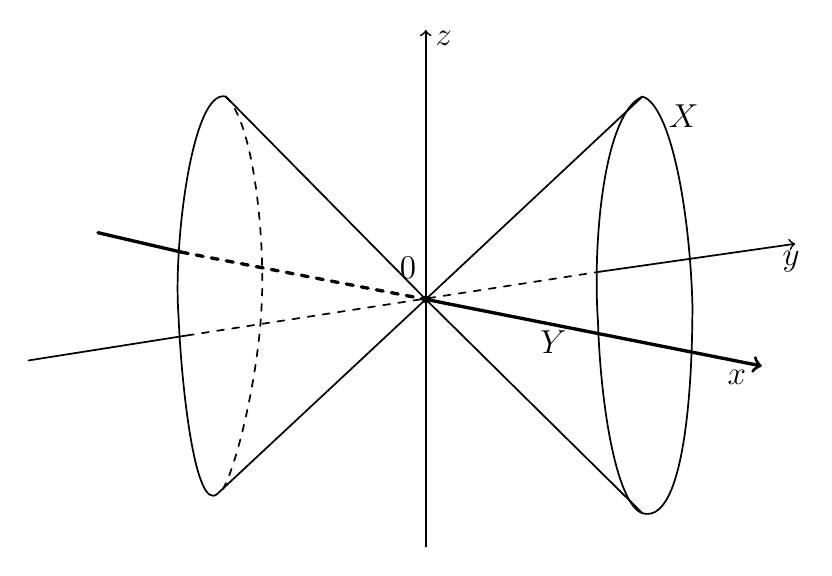
\begin{tikzpicture}[x=1bp,y=-1bp,line cap=round,line join=round,
    outline/.style={line width=.62bp},
    hidden/.style={dash pattern=on 2.5bp off 3bp},
    every node/.style={inner sep=1.3bp,font=\large}]
  % Coordinate axes and the ruling in the x-direction.
  \draw[outline,->] (143,188) -- (143,2);
  \draw[outline] (0,121) -- (57,112);
  \draw[outline,hidden] (57,112) -- (206,89);
  \draw[outline,->] (206,89) -- (276,79);
  \draw[line width=1.2bp] (25,75) -- (55,82);
  \draw[line width=1.2bp,hidden] (55,82) -- (143,99);
  \draw[line width=1.2bp,->] (143,99) -- (264,123);
  % The two sheets and the visible and hidden rims.
  \draw[outline] (143,99) -- (71,26);
  \draw[outline] (143,99) -- (68,169);
  \draw[outline] (143,99) -- (221,26);
  \draw[outline] (143,99) -- (221,176);
  \draw[outline] (71,26) .. controls (59,23) and (52,79) .. (54,105)
    .. controls (55,130) and (60,176) .. (68,169);
  \draw[outline,hidden] (71,26) .. controls (81,35) and (85,76) .. (84,99)
    .. controls (83,130) and (72,170) .. (68,169);
  \draw[outline] (221,26) .. controls (207,32) and (203,79) .. (205,107)
    .. controls (206,139) and (212,173) .. (221,176)
    .. controls (235,180) and (239,137) .. (239,101)
    .. controls (238,66) and (231,29) .. (221,26);
  \fill (143,99) circle (1.4bp);
  \node[above left] at (141,93) {$0$};
  \node[below right] at (145,1) {$z$};
  \node[below right] at (270,80) {$y$};
  \node[below] at (255,123) {$x$};
  \node[below] at (189,109) {$Y$};
  \node[right] at (229,33) {$X$};
\end{tikzpicture}}\par
\smallskip
\small\textbf{Figure 8.}\enspace A ruling on the quadric cone.\par
}
\medskip
\noindent where the first map sends $1\mapsto1\cdot Y$. Now $Y$ can be cut out set-theoretically by the function $y$. In fact, the divisor of $y$ is $2\cdot Y$, because $y=0\Rightarrow z^2=0$, and $z$ generates the maximal ideal of the local ring at the generic point of $Y$. Hence $X-Y=\operatorname{Spec} A_y$. Now $A_y=k[x,y,y^{-1},z]/(xy-z^2)$. In this ring $x=y^{-1}z^2$, so we can eliminate $x$, and find $A_y\cong k[y,y^{-1},z]$. This is a UFD, so by (\Goto{result-II-6.2}{6.2}), $\operatorname{Cl}(X-Y)=0$.

Thus we see that $\operatorname{Cl} X$ is generated by $Y$, and that $2\cdot Y=0$. It remains to show that $Y$ itself is not a principal divisor. \EditionText{Identify $A$ with $k[u^2,uv,v^2]$, the even-degree subring of $k[u,v]$. If an element of $\operatorname{Frac}A$ is integral over $A$, it lies in $k[u,v]$ by normality of that polynomial ring. Writing the element as $g/h$ with $g,h\in A$ and $h\ne0$ shows that its odd-degree part vanishes, since multiplication by the nonzero even-degree polynomial $h$ preserves parity. Thus $A$ is integrally closed, and it is equivalent} to show that the prime ideal of $Y$, namely $\mathfrak p=(y,z)$, is not principal (cf.\ proof of (\Goto{result-II-6.2}{6.2})). Let $\mathfrak m=(x,y,z)$, and note that $\mathfrak m/\mathfrak m^2$ is a $3$-dimensional vector space over $k$ generated by $\bar x,\bar y,\bar z$, the images of $x,y,z$. Now $\mathfrak p\subseteq\mathfrak m$, and the image of $\mathfrak p$ in $\mathfrak m/\mathfrak m^2$ contains $\bar y$ and $\bar z$. Hence $\mathfrak p$ cannot be a principal ideal.

\medskip
\noindent\hypertarget{result-II-6.6}{}\textbf{Proposition 6.6.} \emph{Let $X$ satisfy \Goto{cond-II-6-star}{$(*)$}. Then $X\times\AffSpace{1}\ ({}=X\times_{\operatorname{Spec}\mathbb Z}\operatorname{Spec}\mathbb Z[t])$ also satisfies \Goto{cond-II-6-star}{$(*)$}, and $\operatorname{Cl} X\cong\operatorname{Cl}(X\times\AffSpace{1})$.}

\smallskip
\noindent\textsc{Proof.} Clearly $X\times\AffSpace{1}$ is noetherian, integral, and separated. To see that it is regular in codimension one, we note that there are two kinds of points of codimension one on $X\times\AffSpace{1}$. \hypertarget{type-II-6.6-1}{}Type~1 is a point $x$ whose image in $X$ is a point $y$ of codimension one. In this case $x$ is the generic point of $\pi^{-1}(y)$, where $\pi\colon X\times\AffSpace{1}\to X$ is the projection. Its local ring is $\mathcal O_x\cong\mathcal O_y[t]_{\mathfrak m_y}$, which is clearly a discrete valuation ring, since $\mathcal O_y$ is. The corresponding prime divisor $\overline{\{x\}}$ is just $\pi^{-1}(\overline{\{y\}})$.

\hypertarget{type-II-6.6-2}{}Type~2 is a point $x\in X\times\AffSpace{1}$ of codimension one, whose image in $X$ is the generic point of $X$. In this case $\mathcal O_x$ is a localization of $K[t]$ at some maximal ideal, where $K$ is the function field of $X$. It is a discrete valuation ring because $K[t]$ is a principal ideal domain. Thus $X\times\AffSpace{1}$ also satisfies~\Goto{cond-II-6-star}{$(*)$}.

We define a map $\operatorname{Cl} X\to\operatorname{Cl}(X\times\AffSpace{1})$ by $D=\sum n_iY_i\mapsto\pi^*D=\sum n_i\pi^{-1}(Y_i)$. If $f\in K^*$, then $\pi^*((f))$ is the divisor of $f$ considered as an element of $K(t)$, the function field of $X\times\AffSpace{1}$. Thus we have a homomorphism $\pi^*\colon\operatorname{Cl} X\to\operatorname{Cl}(X\times\AffSpace{1})$.}
% Contents from body/page-149.tex.
\ChapterSheet{149}{135}{\Goto{sec-II-6}{6\quad Divisors}}{%
To show $\pi^*$ is injective, suppose $D\in\operatorname{Div} X$, and $\pi^*D=(f)$ for some $f\in K(t)$. Since $\pi^*D$ involves only prime divisors of type~\Goto{type-II-6.6-1}{1}, $f$ must be in $K$. For otherwise we could write $f=g/h$, with $g,h\in K[t]$, relatively prime. If $g,h$ are not both in $K$, then $(f)$ will involve some prime divisor of type~\Goto{type-II-6.6-2}{2} on $X\times\AffSpace{1}$. Now if $f\in K$, it is clear that $D=(f)$, so $\pi^*$ is injective.

To show that $\pi^*$ is surjective, it will be sufficient to show that any prime divisor of type~\Goto{type-II-6.6-2}{2} on $X\times\AffSpace{1}$ is linearly equivalent to a linear combination of prime divisors of type~\Goto{type-II-6.6-1}{1}. So let $Z\subseteq X\times\AffSpace{1}$ be a prime divisor of type~\Goto{type-II-6.6-2}{2}. Localizing at the generic point of $X$, we get a prime divisor in $\operatorname{Spec} K[t]$, which corresponds to a prime ideal $\mathfrak p\subseteq K[t]$. This is principal, so let $f$ be a generator. Then $f\in K(t)$, and the divisor of $f$ consists of $Z$ plus perhaps something purely of type~\Goto{type-II-6.6-1}{1}. It cannot involve any other prime divisors of type~\Goto{type-II-6.6-2}{2}. Thus $Z$ is linearly equivalent to a divisor purely of type~\Goto{type-II-6.6-1}{1}. This completes the proof.

\medskip
\noindent\hypertarget{result-II-6.6.1}{}\textbf{Example 6.6.1.} Let $Q$ be the nonsingular quadric surface $xy=zw$ in $\mathbf P_k^3$. We will show that $\operatorname{Cl} Q\cong\mathbb Z\oplus\mathbb Z$. We use the fact that $Q$ is isomorphic to $\mathbf P_k^1\times_k\mathbf P_k^1$ (I, Ex.~\Goto{ex-I-2.15}{2.15}). Let $p_1$ and $p_2$ be the projections of $Q$ onto the two factors. Then as in the proof of (\Goto{result-II-6.6}{6.6}) we obtain homomorphisms $p_1^*,p_2^*\colon \operatorname{Cl}\mathbf P^1\to\operatorname{Cl} Q$. First we show that $p_1^*$ and $p_2^*$ are injective. Let $Y=\mathrm{pt}\times\mathbf P^1$. Then $Q-Y=\AffSpace{1}\times\mathbf P^1$, and the composition
\[
\operatorname{Cl}\mathbf P^1\xrightarrow{p_2^*}\operatorname{Cl} Q\to\operatorname{Cl}(\AffSpace{1}\times\mathbf P^1)
\]
is the isomorphism of (\Goto{result-II-6.6}{6.6}). Hence $p_2^*$ (and similarly $p_1^*$) is injective.

Now consider the exact sequence of (\Goto{result-II-6.5}{6.5}) for $Y$:
\[
\mathbb Z\to\operatorname{Cl} Q\to\operatorname{Cl}(\AffSpace{1}\times\mathbf P^1)\to0.
\]
In this sequence the first map sends $1$ to $Y$. But if we identify $\operatorname{Cl}\mathbf P^1$ with $\mathbb Z$ by letting $1$ be the class of a point, then this first map is just $p_1^*$, hence is injective. Since the image of $p_2^*$ goes isomorphically to $\operatorname{Cl}(\AffSpace{1}\times\mathbf P^1)$ as we have just seen, we conclude that $\operatorname{Cl} Q\cong\operatorname{Im} p_1^*\oplus\operatorname{Im} p_2^*=\mathbb Z\oplus\mathbb Z$. If $D$ is any divisor on $Q$, let $(a,b)$ be the ordered pair of integers in $\mathbb Z\oplus\mathbb Z$ corresponding to the class of $D$ under this isomorphism. Then we say $D$ is of \emph{type $(a,b)$} on $Q$.

\medskip
\noindent\hypertarget{result-II-6.6.2}{}\textbf{Example 6.6.2.} Continuing with the quadric surface $Q\subseteq\mathbf P^3$, we will show that the embedding induces a homomorphism $\operatorname{Cl}\mathbf P^3\to\operatorname{Cl} Q$, and that the image of a hyperplane $H$, which generates $\operatorname{Cl}\mathbf P^3$, is the element $(1,1)$ in $\operatorname{Cl} Q=\mathbb Z\oplus\mathbb Z$. Let $Y$ be any irreducible hypersurface of $\mathbf P^3$ which does not contain $Q$. Then we can assign multiplicities to the irreducible components of $Y\cap Q$ so as to obtain a divisor $Y\cdot Q$ on $Q$. Indeed, on each standard open set $U_i$ of $\mathbf P^3$, $Y$ is defined by a single function $f$; we can take the value of this function (restricted to $Q$) for each valuation of a prime divisor of $Q$ to define the divisor $Y\cdot Q$. By linearity we extend this map to define a}
% Contents from body/page-150.tex.
% Original printed page 136.
\ChapterSheet[11.4]{150}{136}{\Goto{p-74}{II\quad Schemes}}{%
divisor $D\cdot Q$ on $Q$, for each divisor $D=\sum n_iY_i$ on $\mathbf P^3$, such that no $Y_i$ contains $Q$. Clearly linearly equivalent divisors restrict to linearly equivalent divisors. Since any divisor on $\mathbf P^3$ is linearly equivalent to one whose prime divisors don't contain $Q$ by (\Goto{result-II-6.4}{6.4}), we obtain a well-defined homomorphism $\operatorname{Cl}\mathbf P^3\to\operatorname{Cl}Q$. Now if $H$ is the hyperplane $w=0$, then $H\cap Q$ is the divisor consisting of the two lines $x=w=0$ and $y=w=0$. One is in each family (I, Ex.\ \Goto{ex-I-2.15}{2.15}) so $H\cap Q$ is of type $(1,1)$ in $\operatorname{Cl}Q=\mathbf Z\oplus\mathbf Z$. Note that the two families of lines correspond to $\mathit{pt}\times\mathbf P^1$ and $\mathbf P^1\times\mathit{pt}$, so they are of type $(1,0)$ and $(0,1)$.

\AuditItem{result-II-6.6.3}{Example 6.6.3.} Carrying this example one step further, let $C$ be the twisted cubic curve $x=t^3$, $y=u^3$, $z=t^2u$, $w=tu^2$ which lies on $Q$. If $Y$ is the quadric cone $yz=w^2$, then $Y\cap Q=C\cup L$ where $L$ is the line $y=w=0$. Since $Y\sim 2H$ on $\mathbf P^3$, $Y\cap Q$ is a divisor of type $(2,2)$. The line $L$ has type $(1,0)$, so $C$ is of type $(1,2)$. It follows that there does not exist any surface $Y\subseteq\mathbf P^3$, not containing $Q$, such that $Y\cap Q=C$, even set-theoretically! For in that case the divisor $Y\cap Q$ would be $rC$ for some integer $r>0$. This is a divisor of type $(r,2r)$ in $\operatorname{Cl}Q$. But if $Y$ is a surface of degree $d$, then $Y\cap Q$ is of type $(d,d)$, which can never equal $(r,2r)$. Thus $Y$ does not exist.

\AuditItem{result-II-6.6.4}{Example 6.6.4.} We will see later (V, \Goto{result-V-4.8}{4.8}) that if $X$ is a nonsingular cubic surface in $\mathbf P^3$, then $\operatorname{Cl}X\cong\mathbf Z^7$.

\medskip
\textit{Divisors on Curves}\par
\noindent We will illustrate the notion of the divisor class group further by paying special attention to the case of divisors on curves. We will define the degree of a divisor on a curve, and we will show that on a complete nonsingular curve, the degree is stable under linear equivalence. Further study of divisors on curves will be found in Chapter \Goto{p-307}{IV}.

To begin with, we need some preliminary information about curves and morphisms of curves. Recall our conventions about terminology from the end of Section \Goto{sec-II-4}{4}:

\par\smallskip\noindent\textbf{Definition.}\enspace Let $k$ be an algebraically closed field. A \emph{curve} over $k$ is an integral separated scheme $X$ of finite type over $k$, of dimension one. If $X$ is proper over $k$, we say that $X$ is \emph{complete}. If all the local rings of $X$ are regular local rings, we say that $X$ is \emph{nonsingular}.

\AuditItem{result-II-6.7}{Proposition 6.7.} \emph{Let $X$ be a nonsingular curve over $k$ with function field $K$. Then the following conditions are equivalent:}
\begin{enumerate}[label=(\roman*),itemsep=0pt,topsep=3pt,parsep=0pt,leftmargin=2.2em]
\item \emph{$X$ is projective;}
\item \emph{$X$ is complete;}
\item \emph{$X\cong t(C_K)$, where $C_K$ is the abstract nonsingular curve of (I, \S\Goto{sec-I-6}{6}), and $t$ is the functor from varieties to schemes of (\Goto{result-II-2.6}{2.6}).}
\end{enumerate}
}
% Contents from body/page-151.tex.
% Original printed page 137.
\ChapterSheet[11.5]{151}{137}{\Goto{sec-II-6}{6\quad Divisors}}{%
\textsc{Proof.}\par
(i) $\Rightarrow$ (ii) follows from (\Goto{result-II-4.9}{4.9}).

(ii) $\Rightarrow$ (iii). If $X$ is complete, then every discrete valuation ring of $K/k$ has a unique center on $X$ (Ex.\ \Goto{ex-II-4.5}{4.5}). Since the local rings of $X$ at the closed points are all discrete valuation rings, this implies that the closed points of $X$ are in 1-1 correspondence with the discrete valuation rings of $K/k$, namely the points of $C_K$. Thus it is clear that $X\cong t(C_K)$.

(iii) $\Rightarrow$ (i) follows from (I, \Goto{result-I-6.9}{6.9}).

\AuditItem{result-II-6.8}{Proposition 6.8.} \emph{Let $X$ be a complete nonsingular curve over $k$, let $Y$ be any curve over $k$, and let $f\colon X\to Y$ be a morphism. Then either (1) $f(X)=$ a point, or (2) $f(X)=Y$. In case (2), $K(X)$ is a finite extension field of $K(Y)$, $f$ is a finite morphism, and $Y$ is also complete.}

\par\smallskip\noindent\textsc{Proof.}\enspace Since $X$ is complete, $f(X)$ must be closed in $Y$, and proper over $\operatorname{Spec}k$ (Ex.\ \Goto{ex-II-4.4}{4.4}). On the other hand, $f(X)$ is irreducible. Thus either (1) $f(X)=\mathit{pt}$, or (2) $f(X)=Y$, and in case (2), $Y$ is also complete.

In case (2), $f$ is dominant, so it induces an inclusion $K(Y)\subseteq K(X)$ of function fields. Since both fields are finitely generated extension fields of transcendence degree $1$ of $k$, $K(X)$ must be a finite algebraic extension of $K(Y)$. To show that $f$ is a finite morphism, let $V=\operatorname{Spec}B$ be any open affine subset of $Y$. Let $A$ be the integral closure of $B$ in $K(X)$. Then $A$ is a finite $B$-module (I, \Goto{result-I-3.9A}{3.9A}), and $\operatorname{Spec}A$ is isomorphic to an open subset $U$ of $X$ (I, \Goto{result-I-6.7}{6.7}). Clearly $U=f^{-1}V$, so this shows that $f$ is a finite morphism.

\par\smallskip\noindent\textbf{Definition.}\enspace If $f\colon X\to Y$ is a finite morphism of curves, we define the \emph{degree} of $f$ to be the degree of the field extension $[K(X):K(Y)]$.

\medskip
Now we come to the study of divisors on curves. If $X$ is a nonsingular curve, then $X$ satisfies the condition (\Goto{cond-II-6-star}{*}) used above, so we can talk about divisors on $X$. A prime divisor is just a closed point, so an arbitrary divisor can be written $D=\sum n_iP_i$, where the $P_i$ are closed points, and $n_i\in\mathbf Z$. We define the \emph{degree} of $D$ to be $\sum n_i$.

\par\smallskip\noindent\textbf{Definition.}\enspace If $f\colon X\to Y$ is a finite morphism of nonsingular curves, we define a homomorphism $f^*\colon\operatorname{Div}Y\to\operatorname{Div}X$ as follows. For any \EditionText{closed point} $Q\in Y$, let $t\in\mathcal O_Q$ be a \emph{local parameter} at $Q$, i.e., $t$ is an element of $K(Y)$ with $v_Q(t)=1$, where $v_Q$ is the valuation corresponding to the discrete valuation ring $\mathcal O_Q$. We define $f^*Q=\sum_{f(P)=Q}v_P(t)\cdot P$. Since $f$ is a finite morphism, this is a finite sum, so we get a divisor on $X$. Note that $f^*Q$ is independent of the choice of the local parameter $t$. Indeed, if $t'$ is another local parameter at $Q$, then $t'=ut$ where $u$ is a unit in $\mathcal O_Q$. For any point $P\in X$ with $f(P)=Q$, $u$ will be a unit in $\mathcal O_P$, so $v_P(t)=v_P(t')$. We extend the definition by linearity to all divisors on $Y$. One sees easily that $f^*$ preserves linear equivalence, so it induces a homomorphism $f^*\colon\operatorname{Cl}Y\to\operatorname{Cl}X$.
}
% Contents from body/page-152.tex.
% Original printed page 138.
\ChapterSheet[11.3]{152}{138}{\Goto{p-74}{II\quad Schemes}}{%
\AuditItem{result-II-6.9}{Proposition 6.9.} \emph{Let $f\colon X\to Y$ be a finite morphism of nonsingular curves. Then for any divisor $D$ on $Y$ we have $\deg f^*D=\deg f\cdot\deg D$.}

\par\smallskip\noindent\textsc{Proof.}\enspace It will be sufficient to show that for any closed point $Q\in Y$ we have $\deg f^*Q=\deg f$. Let $V=\operatorname{Spec}B$ be an open affine subset of $Y$ containing $Q$. Let $A$ be the integral closure of $B$ in $K(X)$. Then, as in the proof of (\Goto{result-II-6.8}{6.8}), $U=\operatorname{Spec}A$ is the open subset $f^{-1}V$ of $X$. Let $\mathfrak m_Q$ be the maximal ideal of $Q$ in $B$. We localize both $B$ and $A$ with respect to the multiplicative system $S=B-\mathfrak m_Q$, and we obtain a ring extension $\mathcal O_Q\hookrightarrow A'$, where $A'$ is a finitely generated $\mathcal O_Q$-module. Now $A'$ is torsion-free, and has rank equal to $r=[K(X):K(Y)]$, so $A'$ is a free $\mathcal O_Q$-module of rank $r=\deg f$. If $t$ is a local parameter at $Q$, it follows that $A'/tA'$ is a $k$-vector space of dimension $r$.

On the other hand, the points $P_i$ of $X$ such that $f(P_i)=Q$ are in 1-1 correspondence with the maximal ideals $\mathfrak m_i$ of $A'$, and for each $i$, $A'_{\mathfrak m_i}=\mathcal O_{P_i}$. Clearly $tA'=\bigcap_i(tA'_{\mathfrak m_i}\cap A')$, so by the Chinese remainder theorem,
\[
  \dim_k A'/tA'=\sum_i\dim_k A'/(tA'_{\mathfrak m_i}\cap A').
\]
But
\[
  A'/(tA'_{\mathfrak m_i}\cap A')\cong A'_{\mathfrak m_i}/tA'_{\mathfrak m_i}
  =\mathcal O_{P_i}/t\mathcal O_{P_i},
\]
so the dimensions in the sum above are just equal to $v_{P_i}(t)$. But $f^*Q=\sum v_{P_i}(t)\cdot P_i$, so we have shown that $\deg f^*Q=\deg f$ as required.

\AuditItem{result-II-6.10}{Corollary 6.10.} \emph{A principal divisor on a complete nonsingular curve $X$ has degree zero. Consequently the degree function induces a surjective homomorphism $\deg\colon\operatorname{Cl}X\to\mathbf Z$.}

\par\smallskip\noindent\textsc{Proof.}\enspace Let $f\in K(X)^*$. If $f\in k$, then $(f)=0$, so there is nothing to prove. If $f\notin k$, then the inclusion of fields $k(f)\subseteq K(X)$ induces a finite morphism $\varphi\colon X\to\mathbf P^1$. It is a morphism by (I, \Goto{result-I-6.12}{6.12}), and it is finite by (\Goto{result-II-6.8}{6.8}). Now $(f)=\varphi^*(\{0\}-\{\infty\})$. Since $\{0\}-\{\infty\}$ is a divisor of degree $0$ on $\mathbf P^1$, we conclude that $(f)$ has degree $0$ on $X$.

Thus the degree of a divisor on $X$ depends only on its linear equivalence class, and we obtain a homomorphism $\operatorname{Cl}X\to\mathbf Z$ as stated. It is surjective, because the degree of a single point is $1$.

\AuditItem{result-II-6.10.1}{Example 6.10.1.} A complete nonsingular curve $X$ is rational if and only if there exist two distinct points $P,Q\in X$ with $P\sim Q$. Recall that \emph{rational} means birational to $\mathbf P^1$. If $X$ is rational, then in fact it is isomorphic to $\mathbf P^1$ by (\Goto{result-II-6.7}{6.7}). And on $\mathbf P^1$ we have already seen that any two points are linearly equivalent (\Goto{result-II-6.4}{6.4}). Conversely, suppose $X$ has two points $P\ne Q$ with $P\sim Q$. Then there is a rational function $f\in K(X)$ with $(f)=P-Q$. Consider the morphism $\varphi\colon X\to\mathbf P^1$ determined by $f$ as in the proof of (\Goto{result-II-6.10}{6.10}). We have $\varphi^*(\{0\})=P$, so $\varphi$ must be a morphism of degree $1$. In other words, $\varphi$ is birational, so $X$ is rational.
}
% Contents from body/page-153.tex.
% Original printed page 139.
\ChapterSheet[11.25]{153}{139}{\Goto{sec-II-6}{6\quad Divisors}}{%
\AuditItem{result-II-6.10.2}{Example 6.10.2.} Let $X$ be the nonsingular cubic curve $y^2z=x^3-xz^2$ in $\mathbf P_k^2$, with $\operatorname{char}k\ne2$. We have already seen that $X$ is not rational (I, Ex.\ \Goto{ex-I-6.2}{6.2}). Let $\operatorname{Cl}^{\circ}X$ be the kernel of the degree map $\operatorname{Cl}X\to\mathbf Z$. Then from the previous example we know that $\operatorname{Cl}^{\circ}X\ne0$. We will show in fact that there is a natural 1-1 correspondence between the set of closed points of $X$ and the elements of the group $\operatorname{Cl}^{\circ}X$. On the one hand this elucidates the structure of the group $\operatorname{Cl}^{\circ}X$. On the other hand it gives us a group structure on the set of closed points of $X$, which makes $X$ into a group variety (Fig.\ \Goto{fig-book-9}{9}).

\par\smallskip\noindent\makebox[\linewidth][c]{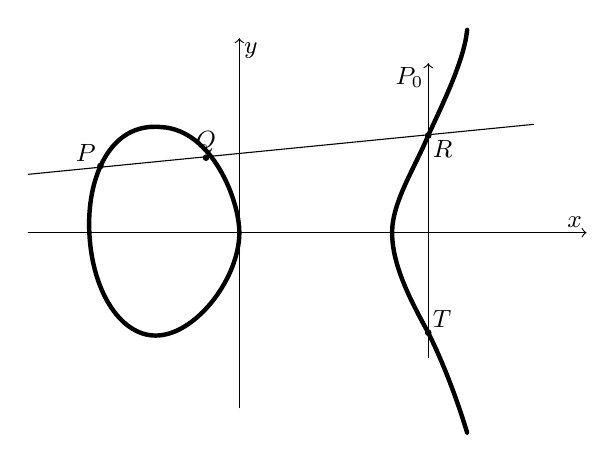
\begin{tikzpicture}[x=1bp,y=-1bp,line cap=round,line join=round,
  every node/.style={inner sep=1.5pt,font=\small}]
  \draw[->] (0,73) -- (201,73) node[above left] {$x$};
  \draw[->] (76,136) -- (76,3) node[below right] {$y$};
  \draw[->] (144,118) -- (144,12) node[below left] {$P_0$};
  \draw (0,52) -- (182,34);
  \draw[line width=1.6pt] (76,73)
    .. controls (76,61) and (66,36) .. (48,35)
    .. controls (29,33) and (21,54) .. (22,73)
    .. controls (23,95) and (34,111) .. (47,110)
    .. controls (61,109) and (76,89) .. cycle;
  \draw[line width=1.6pt] (158,0)
    .. controls (157,11) and (149,27) .. (144,38)
    .. controls (139,50) and (131,62) .. (131,73)
    .. controls (131,85) and (138,98) .. (144,109)
    .. controls (150,121) and (155,135) .. (158,145);
  \foreach \x/\y/\spot/\where in {26/49/P/above left,64/46/Q/above,
      144/38/R/below right,144/109/T/above right}
    \fill (\x,\y) circle[radius=1.2bp] node[\where] {$\spot$};
\end{tikzpicture}
}\par
\noindent\makebox[\linewidth][c]{\small\hypertarget{fig-book-9}{}\textbf{Figure 9.}\enspace The group law on a cubic curve.}\par
\smallskip

Let $P_0$ be the point $(0,1,0)$ on $X$. It is an inflection point, so the tangent line $z=0$ at that point meets the curve in the divisor $3P_0$. If $L$ is any other line in $\mathbf P^2$, meeting $X$ in three points $P,Q,R$ (which may coincide), then since $L$ is linearly equivalent to the line $z=0$ in $\mathbf P^2$, we have $P+Q+R\sim3P_0$ on $X$, as in (\Goto{result-II-6.6.2}{6.6.2}) above.

Now to any closed point $P\in X$, we associate the divisor $P-P_0\in\operatorname{Cl}^{\circ}X$. This map is injective, because if $P-P_0\sim Q-P_0$, then $P\sim Q$, and $X$ would be rational by the previous example, which is impossible.

To show that the map from the closed points of $X$ to $\operatorname{Cl}^{\circ}X$ is surjective, we proceed in several steps. Let $D\in\operatorname{Cl}^{\circ}X$. Then $D=\sum n_iP_i$, with $\sum n_i=0$. Hence we can also write $D=\sum n_i(P_i-P_0)$. Now for any point $R$, let the line $P_0R$ meet $X$ further in the point $T$ (always counting intersections with multiplicities---for example, if $R=P_0$, we take the line $P_0R$ to be the tangent line at $P_0$, and then the third intersection $T$ is also $P_0$). Then $P_0+R+T\sim3P_0$, so $R-P_0\sim-(T-P_0)$. If $i$ is an index such that $n_i<0$ in $D$, we take $P_i=R$. Then replacing $P_i$ by $T$, we get a linearly equivalent divisor with the $i$th coefficient $-n_i>0$. Repeating this process, we may assume that $D=\sum n_i(P_i-P_0)$ with all $n_i>0$. We now show by induction on $\sum n_i$ that $D\sim P-P_0$ for some point $P$. If $\sum n_i=1$, there is nothing to prove. So suppose $\sum n_i\geqslant2$, and let $P,Q$ be two of the points $P_i$ (maybe the same) which occur in $D$. Let the line $PQ$ meet $X$ in $R$, and let the line $P_0R$ meet $X$ in $T$.
}
% Contents from body/page-154.tex.
% Original printed page 140.
\ChapterSheet[11.4]{154}{140}{\Goto{p-74}{II\quad Schemes}}{%
Then we have
\[
  P+Q+R\sim3P_0\qquad\text{and}\qquad P_0+R+T\sim3P_0
\]
so
\[
  (P-P_0)+(Q-P_0)\sim(T-P_0).
\]
Replacing $P$ and $Q$ by $T$, we get $D$ linearly equivalent to another divisor of the same form whose $\sum n_i$ is one less, so by induction $D\sim P-P_0$ for some $P$.

Thus we have shown that the group $\operatorname{Cl}^{\circ}X$ is in 1-1 correspondence with the set of closed points of $X$. One can show directly that the addition law determines a morphism of $X\times X\to X$, and the inverse law determines a morphism $X\to X$ (see for example Olson \Goto{bib-olson-1}{[1]}). Thus $X$ is a group variety in the sense of (I, Ex.\ \Goto{ex-I-3.21}{3.21}). See (IV, \Goto{result-IV-1.3.7}{1.3.7}) for a generalization.

\AuditItem{result-II-6.10.3}{Remark 6.10.3.} This example of the cubic curve illustrates the general fact that the divisor class group of a variety has a discrete component (in this case $\mathbf Z$) and a continuous component (in this case $\operatorname{Cl}^{\circ}X$) which itself has the structure of an algebraic variety.

More specifically, if $X$ is any complete nonsingular curve, then the group $\operatorname{Cl}^{\circ}X$ is isomorphic to the group of closed points of an abelian variety called the \emph{Jacobian variety} of $X$. An \emph{abelian variety} is a complete group variety over $k$. The dimension of the Jacobian variety is the \emph{genus} of the curve. Thus the whole divisor class group of $X$ is an extension of $\mathbf Z$ by the group of closed points of the Jacobian variety of $X$.

If $X$ is a nonsingular projective variety of dimension $\geqslant2$, then one can define a subgroup $\operatorname{Cl}^{\circ}X$ of $\operatorname{Cl}X$, namely the subgroup of divisor classes \emph{algebraically equivalent} to zero, such that $\operatorname{Cl}X/\operatorname{Cl}^{\circ}X$ is a finitely generated abelian group, called the \emph{N\'eron-Severi group} of $X$, and $\operatorname{Cl}^{\circ}X$ is isomorphic to the group of closed points of an abelian variety called the \emph{Picard variety} of $X$.

Unfortunately we do not have space in this book to develop the theory of abelian varieties and to study the Jacobian and Picard varieties of a given variety. For more information and further references on this beautiful subject, see Lang \Goto{bib-lang-1}{[1]}, Mumford \Goto{bib-mumford-2}{[2]}, Mumford \Goto{bib-mumford-5}{[5]}, and Hartshorne \Goto{bib-hartshorne-6}{[6]}. See also (IV, \S\Goto{sec-IV-4}{4}), (V, Ex.\ \Goto{ex-V-1.7}{1.7}), and Appendix \Goto{p-452}{B}.

\medskip
\textit{Cartier Divisors}\par
\noindent Now we want to extend the notion of divisor to an arbitrary scheme. It turns out that using the irreducible subvarieties of codimension one doesn't work very well. So instead, we take as our point of departure the idea that a divisor should be something which locally looks like the divisor of a rational function. This is not exactly a generalization of the Weil divisors (as we will see), but it gives a good notion to use on arbitrary schemes.

\par\smallskip\noindent\textbf{Definition.}\enspace Let $X$ be a scheme. For each open affine subset $U=\operatorname{Spec}A$, let $S$ be the set of elements of $A$ which are not zero divisors, and let $K(U)$ be
}
% Contents from body/page-155.tex.
% Original printed page 141.
\ChapterSheet[11.4]{155}{141}{\Goto{sec-II-6}{6\quad Divisors}}{%
the localization of $A$ by the multiplicative system $S$. We call $K(U)$ the \emph{total quotient ring} of $A$. For each open set $U$, let $S(U)$ denote the set of elements of $\Gamma(U,\mathcal O_X)$ which are not zero divisors in each local ring $\mathcal O_x$ for $x\in U$. Then the rings $S(U)^{-1}\Gamma(U,\mathcal O_X)$ form a presheaf, whose associated sheaf of rings $\mathcal K$ we call the \emph{sheaf of total quotient rings} of $\mathcal O$. On an arbitrary scheme, the sheaf $\mathcal K$ replaces the concept of function field of an integral scheme. We denote by $\mathcal K^*$ the sheaf (of multiplicative groups) of invertible elements in the sheaf of rings $\mathcal K$. Similarly $\mathcal O^*$ is the sheaf of invertible elements in $\mathcal O$.

\par\smallskip\noindent\textbf{Definition.}\enspace A \emph{Cartier divisor} on a scheme $X$ is a global section of the sheaf $\mathcal K^*/\mathcal O^*$. Thinking of the properties of quotient sheaves, we see that a Cartier divisor on $X$ can be described by giving an open cover $\{U_i\}$ of $X$, and for each $i$ an element $f_i\in\Gamma(U_i,\mathcal K^*)$, such that for each $i,j$, $f_i/f_j\in\Gamma(U_i\cap U_j,\mathcal O^*)$. A Cartier divisor is \emph{principal} if it is in the image of the natural map $\Gamma(X,\mathcal K^*)\to\Gamma(X,\mathcal K^*/\mathcal O^*)$. Two Cartier divisors are \emph{linearly equivalent} if their difference is principal. (Although the group operation on $\mathcal K^*/\mathcal O^*$ is multiplication, we will use the language of additive groups when speaking of Cartier divisors, so as to preserve the analogy with Weil divisors.)

\AuditItem{result-II-6.11}{Proposition 6.11.} \emph{Let $X$ be an integral, separated noetherian scheme, all of whose local rings are unique factorization domains (in which case we say $X$ is} locally factorial\emph{). Then the group $\operatorname{Div}X$ of Weil divisors on $X$ is isomorphic to the group of Cartier divisors $\Gamma(X,\mathcal K^*/\mathcal O^*)$, and furthermore, the principal Weil divisors correspond to the principal Cartier divisors under this isomorphism.}

\par\smallskip\noindent\textsc{Proof.}\enspace First note that $X$ is normal, hence satisfies (\Goto{cond-II-6-star}{*}), since a UFD is integrally closed. Thus it makes sense to talk about Weil divisors. Since $X$ is integral, the sheaf $\mathcal K$ is just the constant sheaf corresponding to the function field $K$ of $X$. Now let a Cartier divisor be given by $\{(U_i,f_i)\}$ where $\{U_i\}$ is an open cover of $X$, and $f_i\in\Gamma(U_i,\mathcal K^*)=K^*$. We define the associated Weil divisor as follows. For each prime divisor $Y$, take the coefficient of $Y$ to be $v_Y(f_i)$, where $i$ is any index for which $Y\cap U_i\ne\varnothing$. If $j$ is another such index, then $f_i/f_j$ is invertible on $U_i\cap U_j$, so $v_Y(f_i/f_j)=0$ and $v_Y(f_i)=v_Y(f_j)$. Thus we obtain a well-defined Weil divisor $D=\sum v_Y(f_i)Y$ on $X$. (The sum is finite because $X$ is noetherian!)

Conversely, if $D$ is a Weil divisor on $X$, let $x\in X$ be any point. Then $D$ induces a Weil divisor $D_x$ on the local scheme $\operatorname{Spec}\mathcal O_x$. Since $\mathcal O_x$ is a UFD, $D_x$ is a principal divisor, by (\Goto{result-II-6.2}{6.2}), so let $D_x=(f_x)$ for some $f_x\in K$. Now the principal divisor $(f_x)$ on $X$ has the same restriction to $\operatorname{Spec}\mathcal O_x$ as $D$, hence they differ only at prime divisors which do not pass through $x$. There are only finitely many of these which have a non-zero coefficient in $D$ or $(f_x)$, so there is an open neighborhood $U_x$ of $x$ such that $D$ and $(f_x)$ have the same restriction to $U_x$. Covering $X$ with such open sets $U_x$, the functions $f_x$ give a Cartier divisor on $X$. Note that if $f,f'$ give the same Weil divisor
}
% Contents from body/page-156.tex.
% Original printed page 142.
\ChapterSheet[11.3]{156}{142}{\Goto{p-74}{II\quad Schemes}}{%
on an open set $U$, then $f/f'\in\Gamma(U,\mathcal O^*)$, since $X$ is normal (cf. proof of (\Goto{result-II-6.2}{6.2})). Thus we have a well-defined Cartier divisor.

These two constructions are inverse to each other, so we see that the groups of Weil divisors and Cartier divisors are isomorphic. Furthermore it is clear that the principal divisors correspond to each other.

\AuditItem{result-II-6.11.1A}{Remark 6.11.1A.} Since a regular local ring is UFD (Matsumura \Goto{bib-matsumura-2}{[2, Th.~48, p.~142]}), this proposition applies in particular to any \emph{regular} integral separated noetherian scheme. A scheme is \emph{regular} if all of its local rings are regular local rings.

\AuditItem{result-II-6.11.2}{Remark 6.11.2.} If $X$ is a normal scheme, which is not necessarily locally factorial, we can define a subgroup of $\operatorname{Div}X$ consisting of the locally principal Weil divisors: $D$ is \emph{locally principal} if $X$ can be covered by open sets $U$ such that $D|_U$ is principal for each $U$. Then the above proof shows that the Cartier divisors are the same as the locally principal Weil divisors.

\AuditItem{result-II-6.11.3}{Example 6.11.3.} Let $X$ be the affine quadric cone $\operatorname{Spec}k[x,y,z]/(xy-z^2)$ treated above (\Goto{result-II-6.5.2}{6.5.2}). The ruling $Y$ is a Weil divisor which is not locally principal in the neighborhood of the vertex of the cone. Indeed, our earlier proof shows that its prime ideal $\mathfrak pA_{\mathfrak m}$ is not a principal ideal even in the local ring $A_{\mathfrak m}$. Thus $Y$ does not correspond to a Cartier divisor. On the other hand $2Y$ is locally principal, and in fact principal. So in this case the group of Cartier divisors modulo principal divisors is $0$, whereas $\operatorname{Cl}X\cong\mathbf Z/2\mathbf Z$.

\AuditItem{result-II-6.11.4}{Example 6.11.4.} Let $X$ be the cuspidal cubic curve $y^2z=x^3$ in $\mathbf P_k^2$, with $\operatorname{char}k\ne2$. In this case $X$ does not satisfy (\Goto{cond-II-6-star}{*}), so we cannot talk about Weil divisors on $X$. However, we can talk about the group $\operatorname{CaCl}X$ of Cartier divisor classes modulo principal divisors. Imitating the case of the nonsingular cubic curve (\Goto{result-II-6.10.2}{6.10.2}) we will show:

(a) there is a surjective degree homomorphism $\deg\colon\operatorname{CaCl}X\to\mathbf Z$;

(b) there is a 1-1 correspondence between the set of nonsingular closed points of $X$ and the kernel $\operatorname{CaCl}^{\circ}X$ of the degree map, which makes it into a group variety; and in fact

(c) there is a natural isomorphism of group varieties between $\operatorname{CaCl}^{\circ}X$ and the additive group $\mathbf G_a$ of the field $k$ (I, Ex.\ \Goto{ex-I-3.21}{3.21a}).

To define the degree of a Cartier divisor on $X$, note that any Cartier divisor is linearly equivalent to one whose local function is invertible in some neighborhood of the singular point $Z=(0,0,1)$. Then this Cartier divisor corresponds to a Weil divisor $D=\sum n_iP_i$ on $X-Z$, and we define the degree of the original divisor to be $\deg D=\sum n_i$. The proof of (\Goto{result-II-6.10}{6.10}) shows that if $f\in K$ is invertible at $Z$, then the principal divisor $(f)$ on $X-Z$ has degree $0$. Thus the degree of a Cartier divisor on $X$ is well-defined, and it passes to linear equivalence classes to give a surjective homomorphism $\deg\colon\operatorname{CaCl}X\to\mathbf Z$.
}
% Contents from body/page-157.tex.
% Original printed page 143.
\ChapterSheet[11.5]{157}{143}{\Goto{sec-II-6}{6\quad Divisors}}{%
Now let $P_0$ be the point $(0,1,0)$ as in the case of the nonsingular cubic curve. To each closed point $P\in X-Z$, we associate the Cartier divisor $D_P$ which is $1$ in a neighborhood of $Z$, and which corresponds to the Weil divisor $P-P_0$ on $X-Z$. First note this map is injective: if $P\ne Q$ are two points in $X-Z$, and if $D_P\sim D_Q$, then there is an $f\in K^*$, which is invertible at $Z$, and such that $(f)=P-Q$ on $X-Z$. Then $f$ gives a morphism of $X$ to $\mathbf P^1$, which must be birational. But then the local ring of $Z$ on $X$ would dominate some discrete valuation ring of $\mathbf P^1$, and this is impossible, because $Z$ is a singular point.

To show that every divisor in $\operatorname{CaCl}^{\circ}X$ is linearly equivalent to $D_P$ for some closed point $P\in X-Z$, we proceed exactly as in the case of the nonsingular cubic curve above. The only difference is to note that the geometric constructions $R\mapsto T$ and $P,Q\mapsto R,T$ described above remain inside of $X-Z$. Thus the group $\operatorname{CaCl}^{\circ}X$ is in 1-1 correspondence with the set of closed points of $X-Z$, making it into a group variety.

In this case we are able to identify the group variety as $\mathbf G_a$. Of course, we know that $X$ is a rational curve, and so $X-Z\cong\mathbf A_k^1$ (I, Ex.\ \Goto{ex-I-3.2}{3.2}). But in fact, if we use the right parametrization, the group law corresponds. So define a morphism of $\mathbf G_a=\operatorname{Spec}k[t]$ to $X-Z$ by $t\mapsto(t,1,t^3)$. This is clearly an isomorphism of varieties. Using a little elementary analytic geometry (left to reader!) one shows that if $P=(t,1,t^3)$ and if $Q=(u,1,u^3)$, then the point $T$ constructed above is just $(t+u,1,(t+u)^3)$. So we have an isomorphism of group varieties of $\mathbf G_a$ to $X-Z$ with the group structure of $\operatorname{CaCl}^{\circ}X$.

\medskip
\textit{Invertible Sheaves}\par
\noindent Recall that an \emph{invertible sheaf} on a ringed space $X$ is defined to be a locally free $\mathcal O_X$-module of rank $1$. We will see now that invertible sheaves on a scheme are closely related to divisor classes modulo linear equivalence.

\AuditItem{result-II-6.12}{Proposition 6.12.} \emph{If $\mathcal L$ and $\mathcal M$ are invertible sheaves on a ringed space $X$, so is $\mathcal L\otimes\mathcal M$. If $\mathcal L$ is any invertible sheaf on $X$, then there exists an invertible sheaf $\mathcal L^{-1}$ on $X$ such that $\mathcal L\otimes\mathcal L^{-1}\cong\mathcal O_X$.}

\par\smallskip\noindent\textsc{Proof.}\enspace The first statement is clear, since $\mathcal L$ and $\mathcal M$ are both locally free of rank $1$, and $\mathcal O_X\otimes\mathcal O_X\cong\mathcal O_X$. For the second statement, let $\mathcal L$ be any invertible sheaf, and take $\mathcal L^{-1}$ to be the dual sheaf $\check{\mathcal L}=\mathcal Hom(\mathcal L,\mathcal O_X)$. Then $\check{\mathcal L}\otimes\mathcal L\cong\mathcal Hom(\mathcal L,\mathcal L)=\mathcal O_X$ by (Ex.\ \Goto{ex-II-5.1}{5.1}).

\par\smallskip\noindent\textbf{Definition.}\enspace For any ringed space $X$, we define the \emph{Picard group} of $X$, $\operatorname{Pic}X$, to be the group of isomorphism classes of invertible sheaves on $X$, under the operation $\otimes$. The proposition shows that in fact it is a group.

\AuditItem{result-II-6.12.1}{Remark 6.12.1.} We will see later (III, Ex.\ \Goto{ex-III-4.5}{4.5}) that $\operatorname{Pic}X$ can be expressed as the cohomology group $H^1(X,\mathcal O_X^*)$.
}
% Contents from body/page-158.tex.
% Original printed page 144.
\ChapterSheet[11.45]{158}{144}{\Goto{p-74}{II\quad Schemes}}{%
\textbf{Definition.}\enspace Let $D$ be a Cartier divisor on a scheme $X$, represented by $\{(U_i,f_i)\}$ as above. We define a subsheaf $\mathcal L(D)$ of the sheaf of total quotient rings $\mathcal K$ by taking $\mathcal L(D)$ to be the sub-$\mathcal O_X$-module of $\mathcal K$ generated by $f_i^{-1}$ on $U_i$. This is well-defined, since $f_i/f_j$ is invertible on $U_i\cap U_j$, so $f_i^{-1}$ and $f_j^{-1}$ generate the same $\mathcal O_X$-module. We call $\mathcal L(D)$ the \emph{sheaf associated to $D$}.

\AuditItem{result-II-6.13}{Proposition 6.13.} \emph{Let $X$ be a scheme. Then:}
\begin{enumerate}[label=(\alph*),leftmargin=2.2em,itemsep=0pt,topsep=2pt,parsep=0pt]
\item\hypertarget{result-II-6.13a}{} \emph{for any Cartier divisor $D$, $\mathcal L(D)$ is an invertible sheaf on $X$. The map $D\mapsto\mathcal L(D)$ gives a 1-1 correspondence between Cartier divisors on $X$ and invertible subsheaves of $\mathcal K$;}
\item\hypertarget{result-II-6.13b}{} $\mathcal L(D_1-D_2)\cong\mathcal L(D_1)\otimes\mathcal L(D_2)^{-1}$;
\item\hypertarget{result-II-6.13c}{} \emph{$D_1\sim D_2$ if and only if $\mathcal L(D_1)\cong\mathcal L(D_2)$ as abstract invertible sheaves} (i.e., \emph{disregarding the embedding in $\mathcal K$}).
\end{enumerate}

\noindent\textsc{Proof.}\par
(\Goto{result-II-6.13a}{a}) Since each $f_i\in\Gamma(U_i,\mathcal K^*)$, the map $\mathcal O_{U_i}\to\mathcal L(D)|_{U_i}$ defined by $1\mapsto f_i^{-1}$ is an isomorphism. Thus $\mathcal L(D)$ is an invertible sheaf. The Cartier divisor $D$ can be recovered from $\mathcal L(D)$ together with its embedding in $\mathcal K$, by taking $f_i$ on $U_i$ to be the inverse of a local generator of $\mathcal L(D)$. For any invertible subsheaf of $\mathcal K$, this construction gives a Cartier divisor, so we have a 1-1 correspondence as claimed.

(\Goto{result-II-6.13b}{b}) If $D_1$ is locally defined by $f_i$ and $D_2$ is locally defined by $g_i$, then $\mathcal L(D_1-D_2)$ is locally generated by $f_i^{-1}g_i$, so $\mathcal L(D_1-D_2)=\mathcal L(D_1)\cdot\mathcal L(D_2)^{-1}$ as subsheaves of $\mathcal K$. This product is clearly isomorphic to the abstract tensor product $\mathcal L(D_1)\otimes\mathcal L(D_2)^{-1}$.

(\Goto{result-II-6.13c}{c}) Using (\Goto{result-II-6.13b}{b}), it will be sufficient to show that $D=D_1-D_2$ is principal if and only if $\mathcal L(D)\cong\mathcal O_X$. If $D$ is principal, defined by $f\in\Gamma(X,\mathcal K^*)$, then $\mathcal L(D)$ is globally generated by $f^{-1}$, so sending $1\mapsto f^{-1}$ gives an isomorphism $\mathcal O_X\cong\mathcal L(D)$. Conversely, given such an isomorphism, the image of $1$ gives an element of $\Gamma(X,\mathcal K^*)$ whose inverse will define $D$ as a principal divisor.

\AuditItem{result-II-6.14}{Corollary 6.14.} \emph{On any scheme $X$, the map $D\mapsto\mathcal L(D)$ gives an injective homomorphism of the group $\operatorname{CaCl}X$ of Cartier divisors modulo linear equivalence to $\operatorname{Pic}X$.}

\AuditItem{result-II-6.14.1}{Remark 6.14.1.} The map $\operatorname{CaCl}X\to\operatorname{Pic}X$ may not be surjective, because there may be invertible sheaves on $X$ which are not isomorphic to any invertible subsheaf of $\mathcal K$. For an example of Kleiman, see Hartshorne \Goto{bib-hartshorne-5}{[5, I.1.3, p.~9]}. On the other hand, this map is an isomorphism in most common situations. Nakai \Goto{bib-nakai-2}{[2, p.~301]} has shown that it is an isomorphism whenever $X$ is projective over a field. We will show now that it is an isomorphism if $X$ is integral.
}
% Contents from body/page-159.tex.
% Original printed page 145.
\ChapterSheet[11.45]{159}{145}{\Goto{sec-II-6}{6\quad Divisors}}{%
\AuditItem{result-II-6.15}{Proposition 6.15.} \emph{If $X$ is an integral scheme, the homomorphism $\operatorname{CaCl}X\to\operatorname{Pic}X$ of (\Goto{result-II-6.14}{6.14}) is an isomorphism.}

\par\smallskip\noindent\textsc{Proof.}\enspace We have only to show that every invertible sheaf is isomorphic to a subsheaf of $\mathcal K$, which in this case is the constant sheaf $K$, where $K$ is the function field of $X$. So let $\mathcal L$ be any invertible sheaf, and consider the sheaf $\mathcal L\otimes_{\mathcal O_X}\mathcal K$. On any open set $U$ where $\mathcal L\cong\mathcal O_X$, we have $\mathcal L\otimes\mathcal K\cong\mathcal K$, so it is a constant sheaf on $U$. Now because $X$ is irreducible, it follows that any sheaf whose restriction to each open set of a covering of $X$ is constant, is in fact a constant sheaf. Thus $\mathcal L\otimes\mathcal K$ is isomorphic to the constant sheaf $\mathcal K$, and the natural map $\mathcal L\to\mathcal L\otimes\mathcal K\cong\mathcal K$ expresses $\mathcal L$ as a subsheaf of $\mathcal K$.

\AuditItem{result-II-6.16}{Corollary 6.16.} \emph{If $X$ is a noetherian, integral, separated locally factorial scheme, then there is a natural isomorphism $\operatorname{Cl}X\cong\operatorname{Pic}X$.}

\par\smallskip\noindent\textsc{Proof.}\enspace This follows from (\Goto{result-II-6.11}{6.11}) and (\Goto{result-II-6.15}{6.15}).

\AuditItem{result-II-6.17}{Corollary 6.17.} \emph{If $X=\mathbf P_k^n$ for some field $k$, then every invertible sheaf on $X$ is isomorphic to $\mathcal O(l)$ for some $l\in\mathbf Z$.}

\par\smallskip\noindent\textsc{Proof.}\enspace \EditionText{For $n=0$, $X=\operatorname{Spec}k$ and every invertible sheaf on $X$ is trivial. For $n\geqslant1$, by (\Goto{result-II-6.4}{6.4}), $\operatorname{Cl}X\cong\mathbf Z$. }
\EditionText{By (\Goto{result-II-6.16}{6.16}), $\operatorname{Pic}X\cong\mathbf Z$.} Furthermore the generator of $\operatorname{Cl}X$ is a hyperplane, which corresponds to the invertible sheaf $\mathcal O(1)$. Hence $\operatorname{Pic}X$ is the free group generated by $\mathcal O(1)$, and any invertible sheaf $\mathcal L$ is isomorphic to $\mathcal O(l)$ for some $l\in\mathbf Z$.

\medskip
We conclude this section with some remarks about closed subschemes\EditionText{} of a scheme $X$.

\par\smallskip\noindent\textbf{Definition.}\enspace A Cartier divisor on a scheme $X$ is \emph{effective} if it can be represented by $\{(U_i,f_i)\}$ where all the $f_i\in\Gamma(U_i,\mathcal O_{U_i})$. In that case we define the \emph{associated subscheme\EditionText{}} $Y$, to be the closed subscheme defined by the sheaf of ideals $\mathcal I$ which is locally generated by $f_i$.\EditionText{ If $X$ is noetherian, all irreducible components of $Y$ have codimension one in $X$.}

\AuditItem{result-II-6.17.1}{Remark 6.17.1.} Clearly this gives a 1-1 correspondence between effective Cartier divisors on $X$ and \emph{locally principal} closed subschemes $Y$, i.e., subschemes whose sheaf of ideals is locally generated by a single element\EditionText{ which is a non-zero-divisor}. Note also that if $X$ is an integral separated noetherian locally factorial scheme, so that the Cartier divisors correspond to Weil divisors by (\Goto{result-II-6.11}{6.11}), then the effective Cartier divisors correspond exactly to the effective Weil divisors.

\AuditItem{result-II-6.18}{Proposition 6.18.} \emph{Let $D$ be an effective Cartier divisor on a scheme $X$, and let $Y$ be the associated locally principal closed subscheme. Then $\mathcal I_Y\cong\mathcal L(-D)$.}
}
% Contents from body/page-160.tex.
% Original printed page 146.
\ChapterSheet[10.9]{160}{146}{\Goto{p-74}{II\quad Schemes}}{%
\textsc{Proof.}\enspace $\mathcal L(-D)$ is the subsheaf of $\mathcal K$ generated locally by $f_i$. Since $D$ is effective, this is actually a subsheaf of $\mathcal O_X$, which is none other than the ideal sheaf $\mathcal I_Y$ of $Y$.

\par\smallskip\noindent\textsc{Exercises}\par
\AuditItem{ex-II-6.1}{6.1.} Let $X$ be a scheme satisfying (\Goto{cond-II-6-star}{*}). Then $X\times\mathbf P^n$ \EditionText{for $n\geqslant1$ }also satisfies (\Goto{cond-II-6-star}{*}), and $\operatorname{Cl}(X\times\mathbf P^n)\cong(\operatorname{Cl}X)\times\mathbf Z$.

\AuditItem{ex-II-6.2}{*6.2.} \emph{Varieties in Projective Space.} Let $k$ be an algebraically closed field, and let $X$ be a \EditionText{positive-dimensional }closed subvariety of $\mathbf P_k^n$ which is nonsingular in codimension one (hence satisfies (\Goto{cond-II-6-star}{*})). For any divisor $D=\sum n_iY_i$ on $X$, we define the \emph{degree} of $D$ to be $\sum n_i\deg Y_i$, where $\deg Y_i$ is the degree of $Y_i$, considered as a projective variety itself (I, \S\Goto{sec-I-7}{7}).
\begin{enumerate}[label=(\alph*),leftmargin=2.7em,itemsep=0pt,topsep=1pt,parsep=0pt]
\item\hypertarget{ex-II-6.2a}{} Let $V$ be an irreducible hypersurface in $\mathbf P^n$ which does not contain $X$, and let $Y_i$ be the irreducible components of $V\cap X$. They all have codimension $1$ by (I, Ex.\ \Goto{ex-I-1.8}{1.8}). For each $i$, let $f_i$ be a local equation for $V$ on some open set $U_i$ of $\mathbf P^n$ for which $Y_i\cap U_i\ne\varnothing$, and let $n_i=v_{Y_i}(\bar f_i)$, where $\bar f_i$ is the restriction of $f_i$ to $U_i\cap X$. Then we define the \emph{divisor} $V.X$ to be $\sum n_iY_i$. Extend by linearity, and show that this gives a well-defined homomorphism from the subgroup of $\operatorname{Div}\mathbf P^n$ consisting of divisors, none of whose components contain $X$, to $\operatorname{Div}X$.
\item If $D$ is a principal divisor on $\mathbf P^n$, for which $D.X$ is defined as in (\Goto{ex-II-6.2a}{a}), show that $D.X$ is principal on $X$. Thus we get a homomorphism $\operatorname{Cl}\mathbf P^n\to\operatorname{Cl}X$.
\item Show that the integer $n_i$ defined in (\Goto{ex-II-6.2a}{a}) is the same as the intersection multiplicity $i(X,V;Y_i)$ defined in (I, \S\Goto{sec-I-7}{7}). Then use the generalized B\'ezout theorem (I, \Goto{result-I-7.7}{7.7}) to show that for any divisor $D$ on $\mathbf P^n$, none of whose components contain $X$,
\[
  \deg(D.X)=(\deg D)\cdot(\deg X).
\]
\item If $D$ is a principal divisor on $X$, show that there is a rational function $f$ on $\mathbf P^n$ such that $D=(f).X$. Conclude that $\deg D=0$. Thus the degree function defines a homomorphism $\deg\colon\operatorname{Cl}X\to\mathbf Z$. (This gives another proof of (\Goto{result-II-6.10}{6.10}), since any complete nonsingular curve is projective.) Finally, there is a commutative diagram
\[
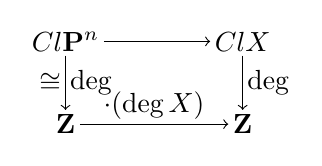
\begin{tikzpicture}[baseline=(current bounding box.center),inner sep=1.5pt]
  \node (A) at (0,1.05) {$\operatorname{Cl}\mathbf P^n$};
  \node (B) at (2.25,1.05) {$\operatorname{Cl}X$};
  \node (C) at (0,0) {$\mathbf Z$};
  \node (D) at (2.25,0) {$\mathbf Z$};
  \draw[->] (A) -- (B);
  \draw[->] (A) -- node[right] {$\deg$} node[left] {$\cong$} (C);
  \draw[->] (B) -- node[right] {$\deg$} (D);
  \draw[->] (C) -- node[above] {$\cdot(\deg X)$} (D);
\end{tikzpicture},
\]
and in particular, we see that the map $\operatorname{Cl}\mathbf P^n\to\operatorname{Cl}X$ is injective.
\end{enumerate}

\AuditItem{ex-II-6.3}{*6.3.} \emph{Cones.} In this exercise we compare the class group of a projective variety $V$ to the class group of its cone (I, Ex.\ \Goto{ex-I-2.10}{2.10}). So let $V$ be a projective variety in $\mathbf P^n$, which is of dimension $\geqslant1$ and nonsingular in codimension $1$. Let $X=C(V)$ be the affine cone over $V$ in $\mathbf A^{n+1}$, and let $\bar X$ be its projective closure in $\mathbf P^{n+1}$. Let $P\in X$ be the vertex of the cone.
\begin{enumerate}[label=(\alph*),leftmargin=2.7em,itemsep=0pt,topsep=1pt,parsep=0pt]
\item Let $\pi\colon\bar X-P\to V$ be the projection map. Show that $V$ can be covered by open subsets $U_i$ such that $\pi^{-1}(U_i)\cong U_i\times\mathbf A^1$ for each $i$, and then show as in (\Goto{result-II-6.6}{6.6}) that $\pi^*\colon\operatorname{Cl}V\to\operatorname{Cl}(\bar X-P)$ is an isomorphism. Since $\operatorname{Cl}\bar X\cong\operatorname{Cl}(\bar X-P)$, we have also $\operatorname{Cl}V\cong\operatorname{Cl}\bar X$.
\end{enumerate}
}
% Contents from body/page-161.tex.
% Original printed page 147.
\ChapterSheet[10.25]{161}{147}{\Goto{sec-II-6}{6\quad Divisors}}{%
\setlength{\parskip}{0pt}%
\begin{enumerate}[start=2,label=(\alph*),leftmargin=2.7em,itemsep=0pt,topsep=1pt,parsep=0pt]
\item We have $V\subseteq\bar X$ as the hyperplane section at infinity. Show that the class of the divisor $V$ in $\operatorname{Cl}\bar X$ is equal to $\pi^*(\text{class of }V.H)$ where $H$ is any hyperplane of $\mathbf P^n$ not containing $V$. Thus conclude using (\Goto{result-II-6.5}{6.5}) that there is an exact sequence
\[
  0\to\mathbf Z\to\operatorname{Cl}V\to\operatorname{Cl}X\to0,
\]
where the first arrow sends $1\mapsto V.H$, and the second is $\pi^*$ followed by the restriction to $X-P$ and inclusion in $X$. (The injectivity of the first arrow follows from the previous exercise.)
\item Let $S(V)$ be the homogeneous coordinate ring of $V$ (which is also the affine coordinate ring of $X$). Show that $S(V)$ is a unique factorization domain if and only if (1) $V$ is projectively normal (Ex.\ \Goto{ex-II-5.14}{5.14}), and (2) $\operatorname{Cl}V\cong\mathbf Z$ and is generated by the class of $V.H$.
\item Let $\mathcal O_P$ be the local ring of $P$ on $X$. Show that the natural restriction map induces an isomorphism $\operatorname{Cl}X\to\operatorname{Cl}(\operatorname{Spec}\mathcal O_P)$.
\end{enumerate}

\AuditItem{ex-II-6.4}{6.4.} Let $k$ be a field of characteristic $\ne2$. Let $f\in k[x_1,\ldots,x_n]$ be a \emph{square-free} nonconstant polynomial, i.e., in the unique factorization of $f$ into irreducible polynomials, there are no repeated factors. Let $A=k[x_1,\ldots,x_n,z]/(z^2-f)$. Show that $A$ is an integrally closed ring. [\emph{Hint:} The quotient field $K$ of $A$ is just $k(x_1,\ldots,x_n)[z]/(z^2-f)$. It is a Galois extension of $k(x_1,\ldots,x_n)$ with Galois group $\mathbf Z/2\mathbf Z$ generated by $z\mapsto-z$. If $\alpha=g+hz\in K$, where $g,h\in k(x_1,\ldots,x_n)$, then the minimal polynomial of $\alpha$ is \EditionText{$X^2-2gX+(g^2-h^2f)$ when $h\ne0$, and $X-g$ when $h=0$.} Now show that $\alpha$ is integral over $k[x_1,\ldots,x_n]$ if and only if $g,h\in k[x_1,\ldots,x_n]$. Conclude that $A$ is the integral closure of $k[x_1,\ldots,x_n]$ in $K$.]

\AuditItem{ex-II-6.5}{*6.5.} \emph{Quadric Hypersurfaces.} Let \EditionText{$k$ be algebraically closed of characteristic $\ne2$}, and let $X$ be the affine quadric hypersurface $\operatorname{Spec}k[x_0,\ldots,x_n]/(x_0^2+x_1^2+\cdots+x_r^2)$---cf. (I, Ex.\ \Goto{ex-I-5.12}{5.12}).
\begin{enumerate}[label=(\alph*),leftmargin=2.7em,itemsep=0pt,topsep=1pt,parsep=0pt]
\item Show that $X$ is normal if $r\geqslant2$ (use Ex.\ \Goto{ex-II-6.4}{6.4}).
\item Show by a suitable linear change of coordinates that the equation of $X$ could be written as $x_0x_1=x_2^2+\cdots+x_r^2$. Now imitate the method of (\Goto{result-II-6.5.2}{6.5.2}) to show that:
\begin{enumerate}[label=(\arabic*),leftmargin=2em,itemsep=0pt,topsep=1pt,parsep=0pt]
\item If $r=2$, then $\operatorname{Cl}X\cong\mathbf Z/2\mathbf Z$;
\item If $r=3$, then $\operatorname{Cl}X\cong\mathbf Z$ (use (\Goto{result-II-6.6.1}{6.6.1}) and (Ex.\ \Goto{ex-II-6.3}{6.3}) above);
\item If $r\geqslant4$ then $\operatorname{Cl}X=0$.
\end{enumerate}
\item Now let $Q$ be the projective quadric hypersurface in $\mathbf P^n$ defined by the same equation. Show that:
\begin{enumerate}[label=(\arabic*),leftmargin=2em,itemsep=0pt,topsep=1pt,parsep=0pt]
\item If $r=2$, $\operatorname{Cl}Q\cong\mathbf Z$, and the class of a hyperplane section $Q.H$ is twice the generator;
\item If $r=3$, $\operatorname{Cl}Q\cong\mathbf Z\oplus\mathbf Z$;
\item If $r\geqslant4$, $\operatorname{Cl}Q\cong\mathbf Z$, generated by $Q.H$.
\end{enumerate}
\item Prove Klein's theorem, which says that if $r\geqslant4$, and if $Y$ is an irreducible subvariety of codimension $1$ on $Q$, then there is an irreducible hypersurface $V\subseteq\mathbf P^n$ such that $V\cap Q=Y$, with multiplicity one. In other words, $Y$ is a complete intersection. (First show that for $r\geqslant4$, the homogeneous coordinate ring $S(Q)=k[x_0,\ldots,x_n]/(x_0^2+\cdots+x_r^2)$ is a UFD.)
\end{enumerate}

\AuditItem{ex-II-6.6}{6.6.} Let $X$ be the nonsingular plane cubic curve $y^2z=x^3-xz^2$ of (\Goto{result-II-6.10.2}{6.10.2}).
\begin{enumerate}[label=(\alph*),leftmargin=2.7em,itemsep=0pt,topsep=1pt,parsep=0pt]
\item Show that three points $P,Q,R$ of $X$ are collinear if and only if $P+Q+R=0$ in the group law on $X$. (Note that the point $P_0=(0,1,0)$ is the zero element in the group structure on $X$.)
\end{enumerate}
}
% Contents from body/page-162.tex.
% Original printed page 148.
\ChapterSheet[10.25]{162}{148}{\Goto{p-74}{II\quad Schemes}}{%
\setlength{\parskip}{0pt}\setlength{\abovedisplayskip}{2pt}\setlength{\belowdisplayskip}{2pt}%
\begin{enumerate}[start=2,label=(\alph*),leftmargin=2.7em,itemsep=0pt,topsep=1pt,parsep=0pt]
\item \EditionText{A point $P\in X$ satisfies $2P=0$ in the group law on $X$ if and only if the tangent line at $P$ passes through $P_0$.}
\item \EditionText{A point $P\in X$ satisfies $3P=0$ in the group law on $X$ if and only if $P$ is an inflection point.} (An \emph{inflection point} of a plane curve is a nonsingular point $P$ of the curve, whose tangent line (I, Ex.\ \Goto{ex-I-7.3}{7.3}) has intersection multiplicity $\geqslant3$ with the curve at $P$.)
\item Let $k=\mathbf C$. Show that the points of $X$ with coordinates in $\mathbf Q$ form a subgroup of the group $X$. Can you determine the structure of this subgroup explicitly?
\end{enumerate}

\AuditItem{ex-II-6.7}{*6.7.} Let $X$ be the nodal cubic curve $y^2z=x^3+x^2z$ in $\mathbf P^2$\EditionText{ over $k$ of characteristic $\ne2$}. Imitate (\Goto{result-II-6.11.4}{6.11.4}) and show that the group of Cartier \EditionText{divisor classes} of degree $0$, $\operatorname{CaCl}^{\circ}X$, is naturally isomorphic to the multiplicative group $\mathbf G_m$.

\AuditItem{ex-II-6.8}{6.8.} \hangindent=2.7em (a) Let $f\colon X\to Y$ be a morphism of schemes. Show that $\mathcal L\mapsto f^*\mathcal L$ induces a homomorphism of Picard groups, $f^*\colon\operatorname{Pic}Y\to\operatorname{Pic}X$.
\par\begin{enumerate}[start=2,label=(\alph*),leftmargin=2.7em,itemsep=0pt,topsep=1pt,parsep=0pt]
\item If $f$ is a finite morphism of nonsingular curves, show that this homomorphism corresponds to the homomorphism $f^*\colon\operatorname{Cl}Y\to\operatorname{Cl}X$ defined in the text, via the isomorphisms of (\Goto{result-II-6.16}{6.16}).
\item If $X$ is a locally factorial integral closed subscheme of $\mathbf P_k^n$, and if $f\colon X\to\mathbf P^n$ is the inclusion map, then $f^*$ on $\operatorname{Pic}$ agrees with the homomorphism on divisor class groups defined in (Ex.\ \Goto{ex-II-6.2}{6.2}) via the isomorphisms of (\Goto{result-II-6.16}{6.16}).
\end{enumerate}

\AuditItem{ex-II-6.9}{*6.9.} \emph{Singular Curves.} Here we give another method of calculating the Picard group of a singular curve. Let $X$ be a projective curve over $k$, let $\widetilde X$ be its normalization, and let $\pi\colon\widetilde X\to X$ be the projection map (Ex.\ \Goto{ex-II-3.8}{3.8}). For each point $P\in X$, let $\mathcal O_P$ be its local ring, and let $\widetilde{\mathcal O}_P$ be the integral closure of $\mathcal O_P$. We use a $*$ to denote the group of units in a ring.
\begin{enumerate}[label=(\alph*),leftmargin=2.7em,itemsep=0pt,topsep=1pt,parsep=0pt]
\item\hypertarget{ex-II-6.9a}{} Show there is an exact sequence
\[
  0\to\bigoplus_{P\in X}\widetilde{\mathcal O}_P^*/\mathcal O_P^*
    \to\operatorname{Pic}X\xrightarrow{\pi^*}\operatorname{Pic}\widetilde X\to0.
\]
[\emph{Hint:} Represent $\operatorname{Pic}X$ and $\operatorname{Pic}\widetilde X$ as the groups of Cartier divisors modulo principal divisors, and use the exact sequence of sheaves on $X$
\[
  0\to\pi_*\mathcal O_{\widetilde X}^*/\mathcal O_X^*
    \to\mathcal K^*/\mathcal O_X^*
    \to\mathcal K^*/\pi_*\mathcal O_{\widetilde X}^*\to0.\text{]}
\]
\item Use (\Goto{ex-II-6.9a}{a}) to give another proof of the fact that if $X$ is a plane cuspidal cubic curve, then there is an exact sequence
\[
  0\to\mathbf G_a\to\operatorname{Pic}X\to\mathbf Z\to0,
\]
and if $X$ is a plane nodal cubic curve, there is an exact sequence
\[
  0\to\mathbf G_m\to\operatorname{Pic}X\to\mathbf Z\to0.
\]
\end{enumerate}

\AuditItem{ex-II-6.10}{6.10.} \emph{The Grothendieck Group $K(X)$.} Let $X$ be a noetherian scheme. We define $K(X)$ to be the quotient of the free abelian group generated by all the coherent sheaves on $X$, by the subgroup generated by all expressions $\mathcal F-\mathcal F'-\mathcal F''$, whenever there is an exact sequence $0\to\mathcal F'\to\mathcal F\to\mathcal F''\to0$ of coherent sheaves on $X$. If $\mathcal F$ is a coherent sheaf, we denote by $\gamma(\mathcal F)$ its image in $K(X)$.
\begin{enumerate}[label=(\alph*),leftmargin=2.7em,itemsep=0pt,topsep=1pt,parsep=0pt]
\item If $X=\mathbf A_k^1$, then $K(X)\cong\mathbf Z$.
\item If $X$ is any integral scheme, and $\mathcal F$ a coherent sheaf, we define the \emph{rank} of $\mathcal F$ to be $\dim_K\mathcal F_\xi$, where $\xi$ is the generic point of $X$, and $K=\mathcal O_\xi$ is the function
\end{enumerate}
}
% Contents from body/page-163.tex.
% Original printed page 149.
\BookMark{1}{2.7  Projective Morphisms}{sec-II-7}
\ChapterSheet[10.85]{163}{149}{\Goto{sec-II-7}{7\quad Projective Morphisms}}{%
\begingroup\leftskip=2.7em
field of $X$. Show that the rank function defines a surjective homomorphism $\operatorname{rank}\colon K(X)\to\mathbf Z$.\par
\endgroup
\begin{enumerate}[start=3,label=(\alph*),leftmargin=2.7em,itemsep=0pt,topsep=1pt,parsep=0pt]
\item If $Y$ is a closed subscheme of $X$, there is an exact sequence
\[
  K(Y)\to K(X)\to K(X-Y)\to0,
\]
where the first map is extension by zero, and the second map is restriction. [\emph{Hint:} For exactness in the middle, show that if $\mathcal F$ is a coherent sheaf on $X$, whose support is contained in $Y$, then there is a finite filtration $\mathcal F=\mathcal F_0\supseteq\mathcal F_1\supseteq\cdots\supseteq\mathcal F_n=0$, such that each $\mathcal F_i/\mathcal F_{i+1}$ is an $\mathcal O_Y$-module. To show surjectivity on the right, use (Ex.\ \Goto{ex-II-5.15}{5.15}).]

For further information about $K(X)$, and its applications to the generalized Riemann--Roch theorem, see Borel--Serre \Goto{bib-borel-serre-1}{[1]}, Manin \Goto{bib-manin-1}{[1]}, and Appendix \Goto{p-438}{A}.
\end{enumerate}

\AuditItem{ex-II-6.11}{*6.11.} \emph{The Grothendieck Group of a Nonsingular Curve.} Let $X$ be a nonsingular curve over an algebraically closed field $k$. We will show that $K(X)\cong\operatorname{Pic}X\oplus\mathbf Z$, in several steps.
\begin{enumerate}[label=(\alph*),leftmargin=2.7em,itemsep=0pt,topsep=1pt,parsep=0pt]
\item For any divisor $D=\sum n_iP_i$ on $X$, let $\psi(D)=\sum n_i\gamma(k(P_i))\in K(X)$, where $k(P_i)$ is the skyscraper sheaf $k$ at $P_i$ and $0$ elsewhere. If $D$ is an effective divisor, let $\mathcal O_D$ be the structure sheaf of the associated subscheme of codimension $1$, and show that $\psi(D)=\gamma(\mathcal O_D)$. Then use (\Goto{result-II-6.18}{6.18}) to show that for any $D$, $\psi(D)$ depends only on the linear equivalence class of $D$, so $\psi$ defines a homomorphism $\psi\colon\operatorname{Cl}X\to K(X)$.
\item For any coherent sheaf $\mathcal F$ on $X$, show that there exist locally free sheaves $\mathcal E_0$ and $\mathcal E_1$ and an exact sequence $0\to\mathcal E_1\to\mathcal E_0\to\mathcal F\to0$. Let $r_0=\operatorname{rank}\mathcal E_0$, $r_1=\operatorname{rank}\mathcal E_1$, and define $\det\mathcal F=(\bigwedge^{r_0}\mathcal E_0)\otimes(\bigwedge^{r_1}\mathcal E_1)^{-1}\in\operatorname{Pic}X$. Here $\bigwedge$ denotes the exterior power (Ex.\ \Goto{ex-II-5.16}{5.16}). Show that $\det\mathcal F$ is independent of the resolution chosen, and that it gives a homomorphism $\det\colon K(X)\to\operatorname{Pic}X$. Finally show that if $D$ is a divisor, then $\det(\psi(D))=\mathcal L(D)$.
\item If $\mathcal F$ is any coherent sheaf of rank $r$, show that there is a divisor $D$ on $X$ and an exact sequence $0\to\mathcal L(D)^{\oplus r}\to\mathcal F\to\mathcal T\to0$, where $\mathcal T$ is a torsion sheaf. Conclude that if $\mathcal F$ is a sheaf of rank $r$, then $\gamma(\mathcal F)-r\gamma(\mathcal O_X)\in\operatorname{Im}\psi$.
\item Using the maps $\psi$, $\det$, $\operatorname{rank}$, and $1\mapsto\gamma(\mathcal O_X)$ from $\mathbf Z\to K(X)$, show that $K(X)\cong\operatorname{Pic}X\oplus\mathbf Z$.
\end{enumerate}

\AuditItem{ex-II-6.12}{6.12.} Let $X$ be a complete nonsingular curve. Show that there is a unique way to define the \emph{degree} of any coherent sheaf on $X$, $\deg\mathcal F\in\mathbf Z$, such that:
\begin{enumerate}[label=(\arabic*),leftmargin=2.7em,itemsep=0pt,topsep=1pt,parsep=0pt]
\item If $D$ is a divisor, $\deg\mathcal L(D)=\deg D$;
\item If $\mathcal F$ is a \emph{torsion sheaf} (meaning a sheaf whose stalk at the generic point is zero), then $\deg\mathcal F=\sum_{P\in X}\operatorname{length}(\mathcal F_P)$; and
\item If $0\to\mathcal F'\to\mathcal F\to\mathcal F''\to0$ is an exact sequence, then $\deg\mathcal F=\deg\mathcal F'+\deg\mathcal F''$.
\end{enumerate}

\par\medskip\noindent\hypertarget{sec-II-7}{}\textbf{\large 7\enspace Projective Morphisms}\par\smallskip
\noindent In this section we gather together several topics concerned with morphisms of a given scheme to projective space. We will show how a morphism of a scheme $X$ to a projective space is determined by giving an invertible sheaf
}
% Contents from body/page-164.tex.
% Original printed page 150.
\ChapterSheet[11.25]{164}{150}{\Goto{p-74}{II\quad Schemes}}{%
$\mathcal L$ on $X$ and a set of its global sections. We will give some criteria for this morphism to be an immersion. Then we study the closely connected topic of ample invertible sheaves. We also introduce the more classical language of linear systems, which from the point of view of schemes is hardly more than another set of terminology for dealing with invertible sheaves and their global sections. However, the geometric understanding furnished by the concept of linear system is often very valuable. At the end of this section we define the $\mathbf{Proj}$ of a graded sheaf of algebras over a scheme $X$, and we give two important examples, namely the projective bundle $\mathbf P(\mathcal E)$ associated with a locally free sheaf $\mathcal E$, and the definition of blowing up with respect to a coherent sheaf of ideals.

\medskip
\textit{Morphisms to $\mathbf P^n$}\par
\noindent Let $A$ be a fixed ring, and consider the projective space $\mathbf P_A^n=\operatorname{Proj}A[x_0,\ldots,x_n]$ over $A$. On $\mathbf P_A^n$ we have the invertible sheaf $\mathcal O(1)$, and the homogeneous coordinates $x_0,\ldots,x_n$ give rise to global sections $x_0,\ldots,x_n\in\Gamma(\mathbf P_A^n,\mathcal O(1))$. One sees easily that the sheaf $\mathcal O(1)$ is generated by the global sections $x_0,\ldots,x_n$, i.e., the images of these sections generate the stalk $\mathcal O(1)_P$ of the sheaf $\mathcal O(1)$ as a module over the local ring $\mathcal O_P$, for each point $P\in\mathbf P_A^n$.

Now let $X$ be any scheme over $A$, and let $\varphi\colon X\to\mathbf P_A^n$ be an $A$-morphism of $X$ to $\mathbf P_A^n$. Then $\mathcal L=\varphi^*(\mathcal O(1))$ is an invertible sheaf on $X$, and the global sections $s_0,\ldots,s_n$, where $s_i=\varphi^*(x_i)$, $s_i\in\Gamma(X,\mathcal L)$, generate the sheaf $\mathcal L$. Conversely, we will see that $\mathcal L$ and the sections $s_i$ determine $\varphi$.

\AuditItem{result-II-7.1}{Theorem 7.1.} \emph{Let $A$ be a ring, and let $X$ be a scheme over $A$.}
\begin{enumerate}[label=(\alph*),leftmargin=2.2em,itemsep=0pt,topsep=2pt,parsep=0pt]
\item\hypertarget{result-II-7.1a}{} \emph{If $\varphi\colon X\to\mathbf P_A^n$ is an $A$-morphism, then $\varphi^*(\mathcal O(1))$ is an invertible sheaf on $X$, which is generated by the global sections $s_i=\varphi^*(x_i)$, $i=0,1,\ldots,n$.}
\item\hypertarget{result-II-7.1b}{} \emph{Conversely, if $\mathcal L$ is an invertible sheaf on $X$, and if $s_0,\ldots,s_n\in\Gamma(X,\mathcal L)$ are global sections which generate $\mathcal L$, then there exists a unique $A$-morphism $\varphi\colon X\to\mathbf P_A^n$ such that $\mathcal L\cong\varphi^*(\mathcal O(1))$ and $s_i=\varphi^*(x_i)$ under this isomorphism.}
\end{enumerate}

\noindent\textsc{Proof.}\enspace Part (\Goto{result-II-7.1a}{a}) is clear from the discussion above. To prove (\Goto{result-II-7.1b}{b}), suppose given $\mathcal L$ and the global sections $s_0,\ldots,s_n$ which generate it. For each $i$, let $X_i=\{P\in X\mid(s_i)_P\notin\mathfrak m_P\mathcal L_P\}$. Then (as we have seen before) $X_i$ is an open subset of $X$, and since the $s_i$ generate $\mathcal L$, the open sets $X_i$ must cover $X$. We define a morphism from $X_i$ to the standard open set $U_i=\{x_i\ne0\}$ of $\mathbf P_A^n$ as follows. Recall that $U_i\cong\operatorname{Spec}A[y_0,\ldots,y_n]$ where $y_j=x_j/x_i$, with $y_i=1$ omitted. We define a ring homomorphism $A[y_0,\ldots,y_n]\to\Gamma(X_i,\mathcal O_{X_i})$ by sending $y_j\mapsto s_j/s_i$ and making it $A$-linear. This makes sense, because for each $P\in X_i$, $(s_i)_P\notin\mathfrak m_P\mathcal L_P$, and $\mathcal L$ is locally free of rank $1$, so the quotient $s_j/s_i$ is a well-defined element of $\Gamma(X_i,\mathcal O_{X_i})$. Now by (Ex.\ \Goto{ex-II-2.4}{2.4}) this ring homomorphism determines a morphism of schemes (over $A$) $X_i\to U_i$. Clearly these morphisms glue (cf. Step \Goto{proof-II-3.3-step-3}{3} of proof of (\Goto{result-II-3.3}{3.3})), so we obtain a morphism $\varphi\colon X\to\mathbf P_A^n$. It is clear from the construction that $\varphi$ is an $A$-
}
% Contents from body/page-165.tex.
% Original printed page 151.
\ChapterSheet[11.2]{165}{151}{\Goto{sec-II-7}{7\quad Projective Morphisms}}{%
morphism, that $\mathcal L\cong\varphi^*(\mathcal O(1))$, and that the sections $s_i$ correspond to $\varphi^*(x_i)$ under this isomorphism. It is clear that any morphism with these properties must be the one given by the construction, so $\varphi$ is unique.

\par\smallskip\noindent\hypertarget{result-II-7.1.1}{}\textbf{Example 7.1.1} (Automorphisms of $\mathbf P_k^n$). If $\lVert a_{ij}\rVert$ is an invertible $(n+1)\times(n+1)$ matrix of elements of a field $k$, then $x_i'=\sum a_{ij}x_j$ determines an automorphism of the polynomial ring $k[x_0,\ldots,x_n]$ and hence also an automorphism of $\mathbf P_k^n$. If $\lambda\in k$ is a nonzero element, then $\lVert\lambda a_{ij}\rVert$ determines the same automorphism of $\mathbf P_k^n$. So we are led to consider the group $\operatorname{PGL}(n,k)=\operatorname{GL}(n+1,k)/k^*$, which acts as a group of automorphisms of $\mathbf P_k^n$. By considering the points $(1,0,\ldots,0)$, $(0,1,0,\ldots,0)$, $\ldots$, $(0,0,\ldots,1)$, and $(1,1,\ldots,1)$, one sees easily that this group acts faithfully, i.e., if $g\in\operatorname{PGL}(n,k)$ induces the trivial automorphism of $\mathbf P_k^n$, then $g$ is the identity.

Now we will show conversely that every $k$-automorphism of $\mathbf P_k^n$ is an element of $\operatorname{PGL}(n,k)$. This generalizes an earlier result for $\mathbf P_k^1$ (I, Ex.\ \Goto{ex-I-6.6}{6.6}). \EditionText{When $n=0$, both groups are trivial. Assume below that $n\geqslant1$. }So let $\varphi$ be a $k$-automorphism of $\mathbf P_k^n$. We have seen (\Goto{result-II-6.17}{6.17}) that $\operatorname{Pic}\mathbf P_k^n\cong\mathbf Z$ and is generated by $\mathcal O(1)$. The automorphism $\varphi$ induces an automorphism of $\operatorname{Pic}\mathbf P^n$, so $\varphi^*(\mathcal O(1))$ must be a generator of that group, hence isomorphic to either $\mathcal O(1)$ or $\mathcal O(-1)$. But $\mathcal O(-1)$ has no global sections, so we conclude that $\varphi^*(\mathcal O(1))\cong\mathcal O(1)$. Now $\Gamma(\mathbf P^n,\mathcal O(1))$ is a $k$-vector space with basis $x_0,\ldots,x_n$, by (\Goto{result-II-5.13}{5.13}). Since $\varphi$ is an automorphism, the $s_i=\varphi^*(x_i)$ must be another basis of this vector space, so we can write $s_i=\sum a_{ij}x_j$, where $\lVert a_{ij}\rVert$ is an invertible matrix of elements of $k$. Since $\varphi$ is uniquely determined by the $s_i$ according to the theorem, we see that $\varphi$ coincides with the automorphism given by $\lVert a_{ij}\rVert$ as an element of $\operatorname{PGL}(n,k)$.

\AuditItem{result-II-7.1.2}{Example 7.1.2.} If $X$ is a scheme over $A$, $\mathcal L$ an invertible sheaf, and $s_0,\ldots,s_n$ any set of global sections, which do not necessarily generate $\mathcal L$, we can always consider the open set $U\subseteq X$ (possibly empty) over which the $s_i$ do generate $\mathcal L$. Then $\mathcal L|_U$ and the $s_i|_U$ give a morphism $U\to\mathbf P_A^n$. Such is the case for example, if we take $X=\mathbf P_k^{n+1}$, $\mathcal L=\mathcal O(1)$, and $s_i=x_i$, $i=0,\ldots,n$ (omitting $x_{n+1}$). These sections generate everywhere except at the point $(0,0,\ldots,0,1)=P_0$. Thus $U=\mathbf P^{n+1}-P_0$, and the corresponding morphism $U\to\mathbf P^n$ is nothing other than the projection from the point $P_0$ to $\mathbf P^n$ (I, Ex.\ \Goto{ex-I-3.14}{3.14}).

\medskip Next we give some criteria for a morphism to a projective space to be a closed immersion.

\AuditItem{result-II-7.2}{Proposition 7.2.} \emph{Let $\varphi\colon X\to\mathbf P_A^n$ be a morphism of schemes over $A$, corresponding to an invertible sheaf $\mathcal L$ on $X$ and sections $s_0,\ldots,s_n\in\Gamma(X,\mathcal L)$ as above. Then $\varphi$ is a closed immersion if and only if}
\begin{enumerate}[label=(\arabic*),leftmargin=2.2em,itemsep=0pt,topsep=2pt,parsep=0pt]
\item\hypertarget{result-II-7.2-1}{} \emph{each open set $X_i=X_{s_i}$ is affine, and}
\item\hypertarget{result-II-7.2-2}{} \emph{for each $i$, the map of rings $A[y_0,\ldots,y_n]\to\Gamma(X_i,\mathcal O_{X_i})$ defined by $y_j\mapsto s_j/s_i$ is surjective.}
\end{enumerate}
}
% Contents from body/page-166.tex.
% Original printed page 152.
\ChapterSheet[10.8]{166}{152}{\Goto{p-74}{II\quad Schemes}}{%
\textsc{Proof.}\enspace First suppose $\varphi$ is a closed immersion. Then $X_i=X\cap U_i$ is a closed subscheme of $U_i$. Therefore $X_i$ is affine and the corresponding map of rings is surjective by (\Goto{result-II-5.10}{5.10}). Conversely, suppose (\Goto{result-II-7.2-1}{1}) and (\Goto{result-II-7.2-2}{2}) satisfied. Then each $X_i$ is a closed subscheme of $U_i$. Since in any case $X_i=\varphi^{-1}(U_i)$, and the $X_i$ cover $X$, it is clear that $X$ is a closed subscheme of $\mathbf P_A^n$.

\medskip
With more hypotheses, we can give a more local criterion.

\AuditItem{result-II-7.3}{Proposition 7.3.} \emph{Let $k$ be an algebraically closed field, let $X$ be a projective scheme over $k$, and let $\varphi\colon X\to\mathbf P_k^n$ be a morphism} (over $k$) \emph{corresponding to $\mathcal L$ and $s_0,\ldots,s_n\in\Gamma(X,\mathcal L)$ as above. Let $V\subseteq\Gamma(X,\mathcal L)$ be the subspace spanned by the $s_i$. Then $\varphi$ is a closed immersion if and only if}
\begin{enumerate}[label=(\arabic*),leftmargin=2.7em,itemsep=0pt,topsep=2pt,parsep=0pt]
\item\hypertarget{result-II-7.3-1}{} \emph{elements of $V$} separate points, \emph{i.e., for any two distinct closed points $P,Q\in X$, there is an $s\in V$ such that $s\in\mathfrak m_P\mathcal L_P$ but $s\notin\mathfrak m_Q\mathcal L_Q$, or vice versa, and}
\item\hypertarget{result-II-7.3-2}{} \emph{elements of $V$} separate tangent vectors, \emph{i.e., for each closed point $P\in X$, the set $\{s\in V\mid s_P\in\mathfrak m_P\mathcal L_P\}$ spans the $k$-vector space $\mathfrak m_P\mathcal L_P/\mathfrak m_P^2\mathcal L_P$.}
\end{enumerate}

\noindent\textsc{Proof.}\enspace If $\varphi$ is a closed immersion, we think of $X$ as a closed subscheme of $\mathbf P_k^n$. In this case $\mathcal L=\mathcal O_X(1)$, and the vector space $V\subseteq\Gamma(X,\mathcal O_X(1))$ is just spanned by the images of $x_0,\ldots,x_n\in\Gamma(\mathbf P^n,\mathcal O(1))$. Given closed points $P\ne Q$ in $X$, there is a hyperplane containing $P$ but not $Q$. If its equation is $\sum a_ix_i=0$, $a_i\in k$, then $s=\sum a_ix_i$ restricted to $X$ has the right property for (\Goto{result-II-7.3-1}{1}). For (\Goto{result-II-7.3-2}{2}), the hyperplanes passing through $P$ give rise to sections which generate $\mathfrak m_P\mathcal L_P/\mathfrak m_P^2\mathcal L_P$. For simplicity suppose that $P$ is the point $(1,0,0,\ldots,0)$. Then on the open affine $U_0\cong\operatorname{Spec}k[y_1,\ldots,y_n]$, $\mathcal L$ is trivial, $P$ is the point $(0,\ldots,0)$, and $\mathfrak m_P/\mathfrak m_P^2$ is exactly the vector space spanned by $y_1,\ldots,y_n$. We use the hypothesis $k$ algebraically closed to ensure that every closed point of $\mathbf P_k^n$ is of the form $(a_0,\ldots,a_n)$ for suitable $a_i\in k$, hence points can be separated by hyperplanes with coefficients in $k$.

For the converse, let $\varphi\colon X\to\mathbf P^n$ satisfy (\Goto{result-II-7.3-1}{1}) and (\Goto{result-II-7.3-2}{2}). \EditionText{Condition (\Goto{result-II-7.3-1}{1}) gives injectivity on closed points. Since $X$ is projective over $k$, $\varphi$ is proper (\Goto{result-II-4.9}{4.9}, \Goto{result-II-4.8e}{4.8e}) and hence closed. If two points have the same image, their closures both map onto the closure of that image. Every closed point of either closure maps to a closed point, and the other closure contains a closed point over that image. By (\Goto{result-II-7.3-1}{1}) these closed points coincide. Both closures thus have the same closed points. These points are dense in each closure, since $X$ is of finite type over $k$. The closures, and hence their generic points, coincide. Thus $\varphi$ is a homeomorphism onto its closed image.} To show that $\varphi$ is a closed immersion, it remains only to show that the morphism of sheaves $\mathcal O_{\mathbf P^n}\to\varphi_*\mathcal O_X$ is surjective. \EditionText{The morphism $\varphi$ is projective by its closed graph in $X\times_k\mathbf P^n$, so $\varphi_*\mathcal O_X$ is coherent by (\Goto{result-II-5.20}{5.20}). Its cokernel vanishes if it vanishes at closed points. Outside the image the cokernel is zero, so it suffices to show $\mathcal O_{\mathbf P^n,P}\to\mathcal O_{X,P}$ surjective for each closed point $P$ of $X$.} Both local rings have the same residue field $k$, and our hypothesis (\Goto{result-II-7.3-2}{2}) implies that the image of the maximal ideal $\mathfrak m_{\mathbf P^n,P}$ generates $\mathfrak m_{X,P}/\mathfrak m_{X,P}^2$. \EditionText{Coherence of $\varphi_*\mathcal O_X$ gives that $\mathcal O_{X,P}$ is a finitely generated $\mathcal O_{\mathbf P^n,P}$-module.} Now our result is a consequence of the following lemma.
}
% Contents from body/page-167.tex.
% Original printed page 153.
\ChapterSheet[11.3]{167}{153}{\Goto{sec-II-7}{7\quad Projective Morphisms}}{%
\AuditItem{result-II-7.4}{Lemma 7.4.} \emph{Let $f\colon A\to B$ be a local homomorphism of local noetherian rings, such that}
\begin{enumerate}[label=(\arabic*),leftmargin=2.2em,itemsep=0pt,topsep=2pt,parsep=0pt]
\item\hypertarget{result-II-7.4-1}{} \emph{$A/\mathfrak m_A\to B/\mathfrak m_B$ is an isomorphism,}
\item\hypertarget{result-II-7.4-2}{} \emph{$\mathfrak m_A\to\mathfrak m_B/\mathfrak m_B^2$ is surjective, and}
\item\hypertarget{result-II-7.4-3}{} \emph{$B$ is a finitely generated $A$-module.}
\end{enumerate}
\emph{Then $f$ is surjective.}

\par\smallskip\noindent\textsc{Proof.}\enspace Consider the ideal $\mathfrak a=\mathfrak m_AB$ of $B$. We have $\mathfrak a\subseteq\mathfrak m_B$, and by (\Goto{result-II-7.4-2}{2}), $\mathfrak a$ contains a set of generators for $\mathfrak m_B/\mathfrak m_B^2$. Hence by Nakayama's lemma for the local ring $B$ and the $B$-module $\mathfrak m_B$, we conclude that $\mathfrak a=\mathfrak m_B$. Now apply Nakayama's lemma to the $A$-module $B$. By (\Goto{result-II-7.4-3}{3}), $B$ is a finitely generated $A$-module. The element $1\in B$ gives a generator for $B/\mathfrak m_AB=B/\mathfrak m_B=A/\mathfrak m_A$ by (\Goto{result-II-7.4-1}{1}), so we conclude that $1$ also generates $B$ as an $A$-module, i.e., $f$ is surjective.

\medskip
\textit{Ample Invertible Sheaves}\par
\noindent Now that we have seen that a morphism of a scheme $X$ to a projective space can be characterized by giving an invertible sheaf on $X$ and a suitable set of its global sections, we can reduce the study of varieties in projective space to the study of schemes with certain invertible sheaves and given global sections. Recall that in \S\Goto{sec-II-5}{5} we defined a sheaf $\mathcal L$ on $X$ to be \emph{very ample relative to $Y$} (where $X$ is a scheme over $Y$) if there is an immersion $i\colon X\to\mathbf P_Y^n$ for some $n$ such that $\mathcal L\cong i^*\mathcal O(1)$. In case $Y=\operatorname{Spec}A$, this is the same thing as saying that $\mathcal L$ admits a set of global sections $s_0,\ldots,s_n$ such that the corresponding morphism $X\to\mathbf P_A^n$ is an immersion. We have also seen (\Goto{result-II-5.17}{5.17}) that if $\mathcal L$ is a very ample invertible sheaf on a projective scheme $X$ over a noetherian ring $A$, then for any coherent sheaf $\mathcal F$ on $X$, there is an integer $n_0>0$ such that for all $n\geqslant n_0$, $\mathcal F\otimes\mathcal L^n$ is generated by global sections. We will use this last property of being generated by global sections to define the notion of an ample invertible sheaf, which is more general, and in many ways is more convenient to work with than the notion of very ample sheaf.

\par\smallskip\noindent\textbf{Definition.}\enspace An invertible sheaf $\mathcal L$ on a noetherian scheme $X$ is said to be \emph{ample} if for every coherent sheaf $\mathcal F$ on $X$, there is an integer $n_0>0$ (depending on $\mathcal F$) such that for every $n\geqslant n_0$, the sheaf $\mathcal F\otimes\mathcal L^n$ is generated by its global sections. (Here $\mathcal L^n=\mathcal L^{\otimes n}$ denotes the $n$-fold tensor power of $\mathcal L$ with itself.)

\AuditItem{result-II-7.4.1}{Remark 7.4.1.} Note that \textquotedblleft{}ample\textquotedblright{} is an absolute notion, i.e., it depends only on the scheme $X$, whereas \textquotedblleft{}very ample\textquotedblright{} is a relative notion, depending on a morphism $X\to Y$.
}
% Contents from body/page-168.tex.
% Original printed page 154.
\ChapterSheet[11.4]{168}{154}{\Goto{p-74}{II\quad Schemes}}{%
\AuditItem{result-II-7.4.2}{Example 7.4.2.} If $X$ is affine, then any invertible sheaf is ample, because every coherent sheaf on an affine scheme is generated by its global sections (\Goto{result-II-5.16.2}{5.16.2}).

\AuditItem{result-II-7.4.3}{Remark 7.4.3.} Serre's theorem (\Goto{result-II-5.17}{5.17}) asserts that a very ample sheaf $\mathcal L$ on a projective scheme $X$ over a noetherian ring $A$ is ample. The converse is false, but we will see below (\Goto{result-II-7.6}{7.6}) that if $\mathcal L$ is ample, then some tensor power $\mathcal L^m$ of $\mathcal L$ is very ample. Thus \textquotedblleft{}ample\textquotedblright{} can be viewed as a stable version of \textquotedblleft{}very ample.\textquotedblright{}

\AuditItem{result-II-7.4.4}{Remark 7.4.4.} In Chapter \Goto{p-215}{III} we will give a characterization of ample invertible sheaves in terms of the vanishing of certain cohomology groups (III, \Goto{result-III-5.3}{5.3}).

\AuditItem{result-II-7.5}{Proposition 7.5.} \emph{Let $\mathcal L$ be an invertible sheaf on a noetherian scheme $X$. Then the following conditions are equivalent:}
\begin{enumerate}[label=(\roman*),leftmargin=2.2em,itemsep=0pt,topsep=2pt,parsep=0pt]
\item\hypertarget{result-II-7.5-i}{} \emph{$\mathcal L$ is ample;}
\item\hypertarget{result-II-7.5-ii}{} \emph{$\mathcal L^m$ is ample for all $m>0$;}
\item\hypertarget{result-II-7.5-iii}{} \emph{$\mathcal L^m$ is ample for some $m>0$.}
\end{enumerate}
\noindent\textsc{Proof.}\enspace (\Goto{result-II-7.5-i}{i}) $\Rightarrow$ (\Goto{result-II-7.5-ii}{ii}) is immediate from the definition of ample; (\Goto{result-II-7.5-ii}{ii}) $\Rightarrow$ (\Goto{result-II-7.5-iii}{iii}) is trivial. To prove (\Goto{result-II-7.5-iii}{iii}) $\Rightarrow$ (\Goto{result-II-7.5-i}{i}), assume that $\mathcal L^m$ is ample. Given a coherent sheaf $\mathcal F$ on $X$, there exists an $n_0>0$ such that $\mathcal F\otimes(\mathcal L^m)^n$ is generated by global sections for all $n\geqslant n_0$. Considering the coherent sheaf $\mathcal F\otimes\mathcal L$, there exists an $n_1>0$ such that $\mathcal F\otimes\mathcal L\otimes(\mathcal L^m)^n$ is generated by global sections for all $n\geqslant n_1$. Similarly, for each $k=1,2,\ldots,m-1$, there is an $n_k>0$ such that $\mathcal F\otimes\mathcal L^k\otimes(\mathcal L^m)^n$ is generated by global sections for all $n\geqslant n_k$. Now if we take $N=m\cdot\max\{n_i\mid i=0,1,\ldots,m-1\}$, then $\mathcal F\otimes\mathcal L^n$ is generated by global sections for all $n\geqslant N$. Hence $\mathcal L$ is ample.

\AuditItem{result-II-7.6}{Theorem 7.6.} \emph{Let $X$ be a scheme of finite type over a noetherian ring $A$, and let $\mathcal L$ be an invertible sheaf on $X$. Then $\mathcal L$ is ample if and only if $\mathcal L^m$ is very ample over $\operatorname{Spec}A$ for some $m>0$.}

\par\smallskip\noindent\textsc{Proof.}\enspace First suppose $\mathcal L^m$ is very ample for some $m>0$. Then there is an immersion $i\colon X\to\mathbf P_A^n$ such that $\mathcal L^m\cong i^*(\mathcal O(1))$. Let $\bar X$ be the closure of $X$ in $\mathbf P_A^n$. Then $\bar X$ is a projective scheme over $A$, so by (\Goto{result-II-5.17}{5.17}), $\mathcal O_{\bar X}(1)$ is ample on $\bar X$. Now given any coherent sheaf $\mathcal F$ on $X$, it extends by (Ex.\ \Goto{ex-II-5.15}{5.15}) to a coherent sheaf $\bar{\mathcal F}$ on $\bar X$. If $\bar{\mathcal F}\otimes\mathcal O_{\bar X}(l)$ is generated by global sections, then a fortiori $\mathcal F\otimes\mathcal O_X(l)$ is also generated by global sections. Thus we see that $\mathcal L^m$ is ample on $X$, and so by (\Goto{result-II-7.5}{7.5}), $\mathcal L$ is also ample on $X$.

For the converse, suppose that $\mathcal L$ is ample on $X$. Given any $P\in X$, let $U$ be an open affine neighborhood of $P$ such that $\mathcal L|_U$ is free on $U$. Let $Y$ be the closed set $X-U$, and let $\mathcal I_Y$ be its sheaf of ideals with the reduced induced scheme structure. Then $\mathcal I_Y$ is a coherent sheaf on $X$, so for some
}
% Contents from body/page-169.tex.
\ChapterSheet{169}{155}{\Goto{sec-II-7}{7\quad Projective Morphisms}}{%
$n>0$, $\mathcal I_Y\otimes\mathcal L^n$ is generated by global sections. In particular, there is a section $s\in\Gamma(X,\mathcal I_Y\otimes\mathcal L^n)$ such that $s_P\notin\mathfrak m_P(\mathcal I_Y\otimes\mathcal L^n)_P$. Now $\mathcal I_Y\otimes\mathcal L^n$ is a subsheaf of $\mathcal L^n$, so we can think of $s$ as an element of $\Gamma(X,\mathcal L^n)$. If $X_s$ is the open set $\{Q\in X\mid s_Q\notin\mathfrak m_Q\mathcal L_Q^n\}$, then it follows from our choice of $s$ that $P\in X_s$ and that $X_s\subseteq U$. Now $U$ is affine, and $\mathcal L^n|_U$ is trivial, so $s$ induces an element $f\in\Gamma(U,\mathcal O_U)$, and then $X_s=U_f$ is also affine.

Thus we have shown that for any point $P\in X$, there is an $n>0$ and a section $s\in\Gamma(X,\mathcal L^n)$ such that $P\in X_s$ and $X_s$ is affine. Since $X$ is quasi-compact, we can cover $X$ by a finite number of such open affines, corresponding to sections $s_i\in\Gamma(X,\mathcal L^{n_i})$. Replacing each $s_i$ by a suitable power $s_i^k\in\Gamma(X,\mathcal L^{kn_i})$, which doesn't change $X_{s_i}$, we may assume that all $n_i$ are equal to one $n$. Finally, since $\mathcal L^n$ is also ample, and since we are only trying to show that some power of $\mathcal L$ is very ample, we may replace $\mathcal L$ by $\mathcal L^n$. Thus we may assume now that we have global sections $s_1,\ldots,s_k\in\Gamma(X,\mathcal L)$ such that each $X_i=X_{s_i}$ is affine, and the $X_i$ cover $X$.

Now for each $i$, let $B_i=\Gamma(X_i,\mathcal O_{X_i})$. Since $X$ is a scheme of finite type over $A$, each $B_i$ is a finitely generated $A$-algebra (Ex.~\Goto{ex-II-3.3}{3.3}). So let $\{b_{ij}\mid j=1,\ldots,k_i\}$ be a set of generators for $B_i$ as an $A$-algebra. By \Goto{result-II-5.14}{(5.14)}, for each $i,j$, there is an integer $n$ such that $s_i^nb_{ij}$ extends to a global section $c_{ij}\in\Gamma(X,\mathcal L^n)$. We can take one $n$ large enough to work for all $i,j$. Now we take the invertible sheaf $\mathcal L^n$ on $X$, and the sections $\{s_i^n\mid i=1,\ldots,k\}$ and $\{c_{ij}\mid i=1,\ldots,k;\ j=1,\ldots,k_i\}$ and use all these sections to define a morphism (over $A$) $\varphi\colon X\to\Proj_A^N$ as in \Goto{result-II-7.1}{(7.1)} above. Since $X$ is covered by the $X_i$, the sections $s_i^n$ already generate the sheaf $\mathcal L^n$, so this is indeed a morphism.

Let $\{x_i\mid i=1,\ldots,k\}$ and $\{x_{ij}\mid i=1,\ldots,k;\ j=1,\ldots,k_i\}$ be the homogeneous coordinates of $\Proj_A^N$ corresponding to the sections of $\mathcal L^n$ mentioned above. For each $i=1,\ldots,k$, let $U_i\subseteq\Proj_A^N$ be the open subset $x_i\ne0$. Then $\varphi^{-1}(U_i)=X_i$, and the corresponding map of affine rings
\[
A[\{y_i\};\{y_{ij}\}]\to B_i
\]
is surjective, because $y_{ij}\mapsto c_{ij}/s_i^n=b_{ij}$, and we chose the $b_{ij}$ so as to generate $B_i$ as an $A$-algebra. Thus $X_i$ is mapped onto a closed subscheme of $U_i$. It follows that $\varphi$ gives an isomorphism of $X$ with a closed subscheme of $\bigcup_{i=1}^kU_i\subseteq\Proj_A^N$, so $\varphi$ is an immersion. Hence $\mathcal L^n$ is very ample relative to $\operatorname{Spec}A$, as required.

\medskip
\noindent\hypertarget{result-II-7.6.1}{}\textbf{Example 7.6.1.} Let $X=\Proj_k^n$, where $k$ is a field. Then $\mathcal O(1)$ is very ample by definition. For any $d>0$, $\mathcal O(d)$ corresponds to the $d$-uple embedding (Ex.~\Goto{ex-II-5.13}{5.13}), so $\mathcal O(d)$ is also very ample. Hence $\mathcal O(d)$ is ample for all $d>0$.
\EditionText{For $n\geq1$ and $l\leq0$, $\mathcal O(-1)\otimes\mathcal O(l)^{\otimes m}=\mathcal O(ml-1)$ has no nonzero global sections for $m>0$, so $\mathcal O(l)$ cannot be ample. Thus on $\Proj_k^n$ for $n\geq1$, $\mathcal O(l)$ is ample $\Leftrightarrow$ very ample $\Leftrightarrow l>0$. On $\Proj_k^0$, every twist is trivial, ample, and very ample.}

\medskip
\noindent\hypertarget{result-II-7.6.2}{}\textbf{Example 7.6.2.} Let $Q$ be the nonsingular quadric surface $xy=zw$ in $\Proj_k^3$ over a field $k$. We have seen \Goto{result-II-6.6.1}{(6.6.1)} that $\operatorname{Pic}Q\cong\mathbf Z\oplus\mathbf Z$, and so we speak
}
% Contents from body/page-170.tex.
\ChapterSheet{170}{156}{\Goto{p-74}{II\quad Schemes}}{%
of the \emph{type} $(a,b)$, $a,b\in\mathbf Z$, of an invertible sheaf. Now $Q\cong\Proj^1\times\Proj^1$. If $a,b>0$, then we consider an $a$-uple embedding $\Proj^1\to\Proj^{n_1}$ and a $b$-uple embedding $\Proj^1\to\Proj^{n_2}$. Taking their product, and following with a Segre embedding, we obtain a closed immersion
\[
Q=\Proj^1\times\Proj^1\to\Proj^{n_1}\times\Proj^{n_2}\to\Proj^n,
\]
which corresponds to an invertible sheaf of type $(a,b)$ on $Q$. Thus for any $a,b>0$, the corresponding invertible sheaf is very ample, and hence ample.
\EditionText{On the other hand, if either $a\leq0$ or $b\leq0$, take a fibre $i\colon F\hookrightarrow Q$, $F\cong\Proj^1$, on which $\mathcal L$ has degree $d\leq0$. Twisting the coherent sheaf $i_*\mathcal O_F(-1)$ by $\mathcal L^{\otimes m}$ gives $i_*\mathcal O_F(md-1)$, which has no nonzero global sections for $m>0$. Thus $\mathcal L$ cannot be ample.}
So on $Q$, an invertible sheaf $\mathcal L$ of type $(a,b)$ is ample $\Leftrightarrow$ very ample $\Leftrightarrow a,b>0$.

\medskip
\noindent\hypertarget{result-II-7.6.3}{}\textbf{Example 7.6.3.} Let $X$ be the nonsingular cubic curve $y^2z=x^3-xz^2$ in $\Proj_k^2$, which was studied in \Goto{result-II-6.10.2}{(6.10.2)}. Let $\mathcal L$ be the invertible sheaf $\mathcal L(P_0)$. Then $\mathcal L$ is ample, because $\mathcal L(3P_0)\cong\mathcal O_X(1)$ is very ample. On the other hand, $\mathcal L$ is not very ample, because $\mathcal L(P_0)$ is not generated by global sections. If it were, then $P_0$ would be linearly equivalent to some other point $Q\in X$, which is impossible, since $X$ is not rational \Goto{result-II-6.10.1}{(6.10.1)}. This shows that an ample sheaf need not be very ample.

\medskip
\noindent\hypertarget{result-II-7.6.4}{}\textbf{Example 7.6.4.} We will see later (IV, \Goto{result-IV-3.3}{3.3}) that if $D$ is a divisor on a complete nonsingular curve $X$, then $\mathcal L(D)$ is ample if and only if $\deg D>0$. This is a consequence of the Riemann--Roch theorem.

\bigskip
\indent\textit{Linear Systems}\par\nobreak\smallskip
\noindent We will see in a minute how global sections of an invertible sheaf correspond to effective divisors on a variety. Thus giving an invertible sheaf and a set of its global sections is the same as giving a certain set of effective divisors, all linearly equivalent to each other. This leads to the notion of linear system, which is the historically older notion. For simplicity, we will employ this terminology only when dealing with nonsingular projective varieties over an algebraically closed field. Over more general schemes the geometrical intuition associated with the concept of linear system may lead one astray, so it is safer to deal with invertible sheaves and their global sections in that case.

So let $X$ be a nonsingular projective variety over an algebraically closed field $k$. In this case the notions of Weil divisor and Cartier divisor are equivalent \Goto{result-II-6.11}{(6.11)}. Furthermore, we have a one-to-one correspondence between linear equivalence classes of divisors and isomorphism classes of invertible sheaves \Goto{result-II-6.15}{(6.15)}. Another useful fact in this situation is that for any invertible sheaf $\mathcal L$ on $X$, the global sections $\Gamma(X,\mathcal L)$ form a finite-dimensional $k$-vector space \Goto{result-II-5.19}{(5.19)}.
}
% Contents from body/page-171.tex.
\ChapterSheet{171}{157}{\Goto{sec-II-7}{7\quad Projective Morphisms}}{%
\indent Let $\mathcal L$ be an invertible sheaf on $X$, and let $s\in\Gamma(X,\mathcal L)$ be a nonzero section of $\mathcal L$. We define an effective divisor $D=(s)_0$, the \emph{divisor of zeros} of $s$, as follows. Over any open set $U\subseteq X$ where $\mathcal L$ is trivial, let $\varphi\colon\mathcal L|_U\xrightarrow{\sim}\mathcal O_U$ be an isomorphism. Then $\varphi(s)\in\Gamma(U,\mathcal O_U)$. As $U$ ranges over a covering of $X$, the collection $\{U,\varphi(s)\}$ determines an effective Cartier divisor $D$ on $X$. Indeed, $\varphi$ is determined up to multiplication by an element of $\Gamma(U,\mathcal O_U^*)$, so we get a well-defined Cartier divisor.

\medskip
\noindent\hypertarget{result-II-7.7}{}\textbf{Proposition 7.7.} \emph{Let $X$ be a nonsingular projective variety over the algebraically closed field $k$. Let $D_0$ be a divisor on $X$ and let $\mathcal L\cong\mathcal L(D_0)$ be the corresponding invertible sheaf. Then:}
\par{\itshape\leftskip=11pt
\hypertarget{result-II-7.7a}{}(a) for each nonzero $s\in\Gamma(X,\mathcal L)$, the divisor of zeros $(s)_0$ is an effective divisor linearly equivalent to $D_0$;

\hypertarget{result-II-7.7b}{}(b) every effective divisor linearly equivalent to $D_0$ is $(s)_0$ for some $s\in\Gamma(X,\mathcal L)$; and

\hypertarget{result-II-7.7c}{}(c) two \EditionText{nonzero sections} $s,s'\in\Gamma(X,\mathcal L)$ have the same divisor of zeros if and only if there is a $\lambda\in k^*$ such that $s'=\lambda s$.\par}

\smallskip
\noindent\textsc{Proof.}\par
(a) We may identify $\mathcal L$ with the subsheaf $\mathcal L(D_0)$ of $\mathcal K$. Then $s$ corresponds to a rational function $f\in K$. If $D_0$ is locally defined as a Cartier divisor by $\{U_i,f_i\}$ with $f_i\in K^*$, then $\mathcal L(D_0)$ is locally generated by $f_i^{-1}$, so we get a local isomorphism $\varphi\colon\mathcal L(D_0)\to\mathcal O$ by multiplying by $f_i$. So $D=(s)_0$ is locally defined by $f_if$. Thus $D=D_0+(f)$, showing that $D\sim D_0$.

(b) If \EditionText{$D\geq0$} and $D=D_0+(f)$, then $(f)\geq-D_0$. Thus $f$ gives a global section of $\mathcal L(D_0)$ whose divisor of zeros is $D$.

(c) Still using the same construction, if $(s)_0=(s')_0$, then $s$ and $s'$ correspond to rational functions $f,f'\in K$ such that $(f/f')=0$. Therefore $f/f'\in\Gamma(X,\mathcal O_X^*)$. But since $X$ is a projective variety over $k$ algebraically closed, $\Gamma(X,\mathcal O_X)=k$, and so $f/f'\in k^*$ (I, \Goto{result-I-3.4}{3.4}).

\medskip
\noindent\textbf{Definition.} A \emph{complete linear system} on a nonsingular projective variety is defined as the set (maybe empty) of all effective divisors linearly equivalent to some given divisor $D_0$. It is denoted by $|D_0|$.

We see from the proposition that the set $|D_0|$ is in one-to-one correspondence with the set $(\Gamma(X,\mathcal L)-\{0\})/k^*$. This gives $|D_0|$ a structure of the set of closed points of a projective space over $k$.

\medskip
\noindent\textbf{Definition.} A \emph{linear system} $\mathfrak d$ on $X$ is a subset of a complete linear system $|D_0|$ which is a linear subspace for the projective space structure of $|D_0|$. Thus $\mathfrak d$ corresponds to a sub-vector space $V\subseteq\Gamma(X,\mathcal L)$, where $V=\{s\in\Gamma(X,\mathcal L)\mid(s)_0\in\mathfrak d\}\cup\{0\}$. The \emph{dimension} of the linear system $\mathfrak d$ is its dimension as a linear projective variety. Hence $\dim\mathfrak d=\dim V-1$. (Note these dimensions are finite because $\Gamma(X,\mathcal L)$ is a finite-dimensional vector space.)
}
% Contents from body/page-172.tex.
\ChapterSheet{172}{158}{\Goto{p-74}{II\quad Schemes}}{%
\noindent\textbf{Definition.} A point $P\in X$ is a \emph{base point} of a linear system $\mathfrak d$ if $P\in\operatorname{Supp}D$ for all $D\in\mathfrak d$. Here $\operatorname{Supp}D$ means the union of the prime divisors of $D$.

\medskip
\noindent\hypertarget{result-II-7.8}{}\textbf{Lemma 7.8.} \emph{Let $\mathfrak d$ be a linear system on $X$ corresponding to the subspace $V\subseteq\Gamma(X,\mathcal L)$. Then a point $P\in X$ is a base point of $\mathfrak d$ if and only if $s_P\in\mathfrak m_P\mathcal L_P$ for all $s\in V$. In particular, $\mathfrak d$ is base-point-free if and only if $\mathcal L$ is generated by the global sections in $V$.}

\smallskip
\noindent\textsc{Proof.} This follows immediately from the fact that for any \EditionText{nonzero $s\in\Gamma(X,\mathcal L)$}, the support of the divisor of zeros $(s)_0$ is the complement of the open set $X_s$.\EditionText{ The zero section already satisfies $s_P\in\mathfrak m_P\mathcal L_P$ for every $P$.}

\medskip
\noindent\hypertarget{result-II-7.8.1}{}\textbf{Remark 7.8.1.} We can rephrase \Goto{result-II-7.1}{(7.1)} in terms of linear systems as follows: to give a morphism from $X$ to $\Proj_k^n$ it is equivalent to give a linear system $\mathfrak d$ without base points on $X$, and a set of elements $s_0,\ldots,s_n\in V$, which span the vector space $V$. Often we will simply talk about the morphism to projective space determined by a linear system without base points $\mathfrak d$. In this case we understand that $s_0,\ldots,s_n$ should be chosen as a basis of $V$. If we chose a different basis, the corresponding morphism of $X\to\Proj^n$ would only differ by an automorphism of $\Proj^n$.

\medskip
\noindent\hypertarget{result-II-7.8.2}{}\textbf{Remark 7.8.2.} We can rephrase \Goto{result-II-7.3}{(7.3)} in terms of linear systems as follows: Let $\varphi\colon X\to\Proj^n$ be a morphism corresponding to the linear system (without base points) $\mathfrak d$. Then $\varphi$ is a closed immersion if and only if

{\leftskip=16pt
\noindent\hypertarget{cond-II-7.8.2-1}{}\llap{(1)\enspace}$\mathfrak d$ \emph{separates points}, i.e., for any two distinct closed points $P,Q\in X$, there is a $D\in\mathfrak d$ such that $P\in\operatorname{Supp}D$ and $Q\notin\operatorname{Supp}D$, and

\noindent\hypertarget{cond-II-7.8.2-2}{}\llap{(2)\enspace}$\mathfrak d$ \emph{separates tangent vectors}, i.e., given a closed point $P\in X$ and a \EditionText{nonzero tangent vector} $t\in T_P(X)=(\mathfrak m_P/\mathfrak m_P^2)'$, there is a $D\in\mathfrak d$ such that $P\in\operatorname{Supp}D$, but $t\notin T_P(D)$. Here we think of $D$ as a locally principal closed subscheme, in which case the Zariski tangent space $T_P(D)=(\mathfrak m_{P,D}/\mathfrak m_{P,D}^2)'$ is naturally a subspace of $T_P(X)$.\par}

The terminology of \textquotedblleft{}separating points\textquotedblright{} and \textquotedblleft{}separating tangent vectors\textquotedblright{} is perhaps somewhat explained by this geometrical interpretation.

\medskip
\noindent\textbf{Definition.} Let $i\colon Y\hookrightarrow X$ be a closed immersion of nonsingular projective varieties over $k$. If $\mathfrak d$ is a linear system on $X$, we define the \emph{trace} of $\mathfrak d$ on $Y$, denoted $\mathfrak d|_Y$, as follows. The linear system $\mathfrak d$ corresponds to an invertible sheaf $\mathcal L$ on $X$, and a sub-vector space $V\subseteq\Gamma(X,\mathcal L)$. We take the invertible sheaf $i^*\mathcal L=\mathcal L\otimes\mathcal O_Y$ on $Y$, and we let $W\subseteq\Gamma(Y,i^*\mathcal L)$ be the image of $V$ under the natural map $\Gamma(X,\mathcal L)\to\Gamma(Y,i^*\mathcal L)$. Then $i^*\mathcal L$ and $W$ define the linear system $\mathfrak d|_Y$.

One can also describe $\mathfrak d|_Y$ geometrically as follows: it consists of all divisors $D.Y$ (defined as in \Goto{result-II-6.6.2}{(6.6.2)}), where $D\in\mathfrak d$ is a divisor whose support does not contain $Y$.

Note that even if $\mathfrak d$ is a complete linear system, $\mathfrak d|_Y$ may not be complete.
}
% Contents from body/page-173.tex.
\ChapterSheet{173}{159}{\Goto{sec-II-7}{7\quad Projective Morphisms}}{%
\noindent\hypertarget{result-II-7.8.3}{}\textbf{Example 7.8.3.} If $X=\Proj^n$\EditionText{ with $n\geq1$}, then the set of all effective divisors of degree $d>0$ is a complete linear system of dimension $\binom{n+d}{n}-1$. Indeed, it corresponds to the invertible sheaf $\mathcal O(d)$, whose global sections consist exactly of the space of all homogeneous polynomials in $x_0,\ldots,x_n$ of degree $d$. This is a vector space of dimension $\binom{n+d}{n}$, so the dimension of the complete linear system is one less.

\medskip
\noindent\hypertarget{result-II-7.8.4}{}\textbf{Example 7.8.4.} We can rephrase (Ex.~\Goto{ex-II-5.14}{5.14d}) in terms of linear systems as follows: a nonsingular projective variety $X\hookrightarrow\Proj_k^n$ is projectively normal if and only if for every $d>0$, the trace on $X$ of the linear system of all divisors of degree $d$ on $\Proj^n$, is a complete linear system. By slight abuse of language, we say that \textquotedblleft{}the linear system on $X$, cut out by the hypersurfaces of degree $d$ in $\Proj^n$, is complete.\textquotedblright{}

\medskip
\noindent\hypertarget{result-II-7.8.5}{}\textbf{Example 7.8.5.} Recall that the \emph{twisted cubic curve} in $\Proj^3$ was defined by the parametric equations $x_0=t^3$, $x_1=t^2u$, $x_2=tu^2$, $x_3=u^3$. In other words, it is just the $3$-uple embedding of $\Proj^1$ in $\Proj^3$ (I, Ex.~\Goto{ex-I-2.12}{2.12}). We will now show that any nonsingular curve $X$ in $\Proj^3$, of degree $3$, which is not contained in any $\Proj^2$, and which is abstractly isomorphic to $\Proj^1$, can be obtained from the given twisted cubic curve by an automorphism of $\Proj^3$. So we will refer to any such curve as a twisted cubic curve.

Let $X$ be such a curve. The embedding of $X$ in $\Proj^3$ is determined by the linear system $\mathfrak d$ of hyperplane sections of $X$ \Goto{result-II-7.1}{(7.1)}. This is a linear system on $X$ of dimension $3$, because the planes in $\Proj^3$ form a linear system of dimension $3$, and by hypothesis $X$ is not contained in any plane, so the map $\Gamma(\Proj^3,\mathcal O(1))\to\Gamma(X,i^*\mathcal O(1))$ is injective. On the other hand, $\mathfrak d$ is a linear system of degree $3$, since $X$ is a curve of degree $3$. By the \emph{degree} of a linear system on a complete nonsingular curve, we mean the degree of any of its divisors, which is independent of the divisor chosen \Goto{result-II-6.10}{(6.10)}. Now thinking of $X$ as $\Proj^1$, the linear system $\mathfrak d$ must correspond to a $4$-dimensional subspace $V\subseteq\Gamma(\Proj^1,\mathcal O(3))$. But $\Gamma(\Proj^1,\mathcal O(3))$ itself has dimension $4$, so $V=\Gamma(\Proj^1,\mathcal O(3))$ and $\mathfrak d$ is a complete linear system. Since the embedding is determined by the linear system and the choice of basis of $V$ by \Goto{result-II-7.1}{(7.1)}, we conclude that $X$ is the same as the $3$-uple embedding of $\Proj^1$, except for the choice of basis of $V$. This shows that there is an automorphism of $\Proj^3$ sending the given twisted cubic curve to $X$. (See (IV, Ex.~\Goto{ex-IV-3.4}{3.4}) for generalization.)

\medskip
\noindent\hypertarget{result-II-7.8.6}{}\textbf{Example 7.8.6.} We define a \emph{nonsingular rational quartic curve} in $\Proj^3$ to be a nonsingular curve $X$ in $\Proj^3$, of degree $4$, not contained in any $\Proj^2$, and which is abstractly isomorphic to $\Proj^1$. In this case we will see that two such curves need not be obtainable one from the other by an automorphism of $\Proj^3$. To give a morphism of $\Proj^1$ to $\Proj^3$ whose image has degree $4$ and is not contained in any $\Proj^2$, we need a $4$-dimensional subspace $V\subseteq\Gamma(\Proj^1,\mathcal O(4))$. This latter vector space has dimension $5$. So if we choose two different subspaces $V,V'$,
}
% Contents from body/page-174.tex.
\ChapterSheet{174}{160}{\Goto{p-74}{II\quad Schemes}}{%
the corresponding curves in $\Proj^3$ may not be related by an automorphism of $\Proj^3$. To be sure the image is nonsingular, we use the criterion of \Goto{result-II-7.3}{(7.3)}. Thus for example, one sees easily that the subspaces $V=(t^4,t^3u,tu^3,u^4)$ and $V'=(t^4,t^3u+at^2u^2,tu^3,u^4)$ for $a\in k^*$ give nonsingular rational quartic curves in $\Proj^3$ which are not equivalent by an automorphism of $\Proj^3$\EditionText{ when $\operatorname{char}k\ne2$}.

\bigskip
\indent\textbf{Proj}, $\mathbf P(\mathcal E)$, \textit{and Blowing Up}\par\nobreak\smallskip
\noindent Earlier we have defined the Proj of a graded ring. Now we introduce a relative version of this construction, which is the \textbf{Proj} of a sheaf of graded algebras $\mathcal S$ over a scheme $X$. This construction is useful in particular because it allows us to construct the projective space bundle associated to a locally free sheaf $\mathcal E$, and it allows us to give a definition of blowing up with respect to an arbitrary sheaf of ideals. This generalizes the notion of blowing up a point introduced in (I, \Goto{sec-I-4}{\S4}).

For simplicity, we will always impose the following conditions on a scheme $X$ and a sheaf of graded algebras $\mathcal S$ before we define a \textbf{Proj}:

\smallskip
{\leftskip=15pt
\noindent\hypertarget{cond-II-7-dagger}{}\llap{$(\dagger)$\enspace}$X$ is a noetherian scheme, $\mathcal S$ is a quasi-coherent sheaf of $\mathcal O_X$-modules, which has a structure of a sheaf of graded $\mathcal O_X$-algebras. Thus $\mathcal S\cong\bigoplus_{d\geq0}\mathcal S_d$, where $\mathcal S_d$ is the homogeneous part of degree $d$. We assume furthermore that $\mathcal S_0=\mathcal O_X$, that $\mathcal S_1$ is a coherent $\mathcal O_X$-module, and that $\mathcal S$ is locally generated by $\mathcal S_1$ as an $\mathcal O_X$-algebra. (It follows that $\mathcal S_d$ is coherent for all $d\geq0$.)\par}

\medskip
\noindent\textbf{Construction.} Let $X$ be a scheme and $\mathcal S$ a sheaf of graded $\mathcal O_X$-algebras satisfying \Goto{cond-II-7-dagger}{$(\dagger)$}. For each open affine subset $U=\operatorname{Spec}A$ of $X$, let $\mathcal S(U)$ be the graded $A$-algebra $\Gamma(U,\mathcal S|_U)$. Then we consider $\operatorname{Proj}\mathcal S(U)$ and its natural morphism $\pi_U\colon\operatorname{Proj}\mathcal S(U)\to U$. If $f\in A$, and $U_f=\operatorname{Spec}A_f$, then since $\mathcal S$ is quasi-coherent, we see that $\operatorname{Proj}\mathcal S(U_f)\cong\pi_U^{-1}(U_f)$. It follows that if $U,V$ are two open affine subsets of $X$, then $\pi_U^{-1}(U\cap V)$ is naturally isomorphic to $\pi_V^{-1}(U\cap V)$---here we leave some technical details to the reader. These isomorphisms allow us to glue the schemes $\operatorname{Proj}\mathcal S(U)$ together (Ex.~\Goto{ex-II-2.12}{2.12}). Thus we obtain a scheme $\operatorname{\mathbf{Proj}}\mathcal S$ together with a morphism $\pi\colon\operatorname{\mathbf{Proj}}\mathcal S\to X$ such that for each open affine $U\subseteq X$, $\pi^{-1}(U)\cong\operatorname{Proj}\mathcal S(U)$. Furthermore the invertible sheaves $\mathcal O(1)$ on each $\operatorname{Proj}\mathcal S(U)$ are compatible under this construction \Goto{result-II-5.12c}{(5.12c)}, so they glue together to give an invertible sheaf $\mathcal O(1)$ on $\operatorname{\mathbf{Proj}}\mathcal S$, canonically determined by this construction.

\medskip
Thus to any $X,\mathcal S$ satisfying \Goto{cond-II-7-dagger}{$(\dagger)$}, we have constructed the scheme $\operatorname{\mathbf{Proj}}\mathcal S$, the morphism $\pi\colon\operatorname{\mathbf{Proj}}\mathcal S\to X$, and the invertible sheaf $\mathcal O(1)$ on $\operatorname{\mathbf{Proj}}\mathcal S$. Everything we have said about the Proj of a graded ring $S$ can be extended to this relative situation. We will not attempt to do this exhaustively, but will only mention certain aspects of the new situation.
}
% Contents from body/page-175.tex.
\ChapterSheet{175}{161}{\Goto{sec-II-7}{7\quad Projective Morphisms}}{%
\noindent\hypertarget{result-II-7.8.7}{}\textbf{Example 7.8.7.} If $\mathcal S$ is the polynomial algebra $\mathcal S=\mathcal O_X[T_0,\ldots,T_n]$, then $\operatorname{\mathbf{Proj}}\mathcal S$ is just the relative projective space $\Proj_X^n$ with its twisting sheaf $\mathcal O(1)$ defined earlier (\Goto{sec-II-5}{\S5}).

\medskip
\noindent\hypertarget{result-II-7.8.8}{}\textbf{Caution 7.8.8.} In general, $\mathcal O(1)$ may not be very ample on $\operatorname{\mathbf{Proj}}\mathcal S$ relative to $X$. See \Goto{result-II-7.10}{(7.10)} and (Ex.~\Goto{ex-II-7.14}{7.14}).

\medskip
\noindent\hypertarget{result-II-7.9}{}\textbf{Lemma 7.9.} \emph{Let $\mathcal S$ be a sheaf of graded algebras on a scheme $X$ satisfying \Goto{cond-II-7-dagger}{$(\dagger)$}. Let $\mathcal L$ be an invertible sheaf on $X$, and define a new sheaf of graded algebras $\mathcal S'=\mathcal S*\mathcal L$ by $\mathcal S'_d=\mathcal S_d\otimes\mathcal L^d$ for each $d\geq0$. Then $\mathcal S'$ also satisfies \Goto{cond-II-7-dagger}{$(\dagger)$}, and there is a natural isomorphism $\varphi\colon P'=\operatorname{\mathbf{Proj}}\mathcal S'\xrightarrow{\sim}P=\operatorname{\mathbf{Proj}}\mathcal S$, commuting with the projections $\pi$ and $\pi'$ to $X$, and having the property that}
\[
\mathcal O_{P'}(1)\cong\varphi^*\mathcal O_P(1)\otimes\pi'^*\mathcal L.
\]

\smallskip
\noindent\textsc{Proof.} Let $\theta\colon\mathcal O_U\xrightarrow{\sim}\mathcal L|_U$ be a local isomorphism of $\mathcal O_U$ with $\mathcal L|_U$ over a small open affine subset $U$ of $X$. Then $\theta$ induces an isomorphism of graded rings $\mathcal S(U)\cong\mathcal S'(U)$ and hence an isomorphism $\theta^*\colon\operatorname{Proj}\mathcal S'(U)\cong\operatorname{Proj}\mathcal S(U)$. If $\theta_1\colon\mathcal O_U\cong\mathcal L|_U$ is a different local isomorphism, then $\theta$ and $\theta_1$ differ by an element $f\in\Gamma(U,\mathcal O_U^*)$, and the corresponding isomorphism $\mathcal S(U)\cong\mathcal S'(U)$ differs by an automorphism $\psi$ of $\mathcal S(U)$ which consists of multiplying by $f^d$ in degree $d$. This does not affect the set of homogeneous prime ideals in $\mathcal S(U)$, and furthermore, since the structure sheaf of $\operatorname{Proj}\mathcal S(U)$ is formed by elements of degree zero in various localizations of $\mathcal S(U)$, the automorphism $\psi$ of $\mathcal S(U)$ induces the \emph{identity} automorphism of $\operatorname{Proj}\mathcal S(U)$. In other words, the isomorphism $\theta^*$ is independent of the choice of $\theta$. So these local isomorphisms $\theta^*$ glue together to give a natural isomorphism $\varphi\colon\operatorname{\mathbf{Proj}}\mathcal S'\xrightarrow{\sim}\operatorname{\mathbf{Proj}}\mathcal S$, commuting with $\pi$ and $\pi'$. When we form the sheaf $\mathcal O(1)$, however, the automorphism $\psi$ of $\mathcal S(U)$ induces multiplication by $f$ in $\mathcal O(1)$. Thus $\mathcal O_{P'}(1)$ looks like $\mathcal O_P(1)$ modified by the transition functions of $\mathcal L$. Stated precisely, this says $\mathcal O_{P'}(1)\cong\varphi^*\mathcal O_P(1)\otimes\pi'^*\mathcal L$.

\medskip
\noindent\hypertarget{result-II-7.10}{}\textbf{Proposition 7.10.} \emph{Let $X,\mathcal S$ satisfy \Goto{cond-II-7-dagger}{$(\dagger)$}, let $P=\operatorname{\mathbf{Proj}}\mathcal S$, with projection $\pi\colon P\to X$ and invertible sheaf $\mathcal O_P(1)$ constructed above. Then:}
\par{\itshape\leftskip=12pt
\hypertarget{result-II-7.10a}{}(a) $\pi$ is a proper morphism. In particular, it is separated and of finite type;

\hypertarget{result-II-7.10b}{}(b) if $X$ admits an ample invertible sheaf $\mathcal L$, then $\pi$ is a projective morphism, and we can take $\mathcal O_P(1)\otimes\pi^*\mathcal L^n$ to be a very ample invertible sheaf on $P$ over $X$, for suitable $n>0$.\par}

\medskip
\noindent\textsc{Proof.}\par
(a) For each open affine $U\subseteq X$, the morphism $\pi_U\colon\operatorname{Proj}\mathcal S(U)\to U$ is a projective morphism \Goto{result-II-4.8.1}{(4.8.1)}, hence proper \Goto{result-II-4.9}{(4.9)}. But the condition for a morphism to be proper is local on the base \Goto{result-II-4.8}{(4.8f)}, so $\pi$ is proper.
}
% Contents from body/page-176.tex.
\ChapterSheet{176}{162}{\Goto{p-74}{II\quad Schemes}}{%
\indent(b) Let $\mathcal L$ be an ample invertible sheaf on $X$. Then for some $n>0$, $\mathcal S_1\otimes\mathcal L^n$ is generated by global sections. Since $X$ is noetherian and $\mathcal S_1\otimes\mathcal L^n$ is coherent, we can find a finite number of global sections which generate it, in other words we can find a surjective morphism of sheaves $\mathcal O_X^{N+1}\to\mathcal S_1\otimes\mathcal L^n$ for some $N$. This allows us to define a surjective map of sheaves of graded $\mathcal O_X$-algebras $\mathcal O_X[T_0,\ldots,T_N]\to\mathcal S*\mathcal L^n$, which gives rise to a closed immersion $\operatorname{\mathbf{Proj}}\mathcal S*\mathcal L^n\hookrightarrow\operatorname{\mathbf{Proj}}\mathcal O_X[T_0,\ldots,T_N]=\Proj_X^N$ (Ex.~\Goto{ex-II-3.12}{3.12}). But $\operatorname{\mathbf{Proj}}\mathcal S*\mathcal L^n\cong\operatorname{\mathbf{Proj}}\mathcal S$ by \Goto{result-II-7.9}{(7.9)}, and the very ample invertible sheaf induced by this embedding is just $\mathcal O_P(1)\otimes\pi^*\mathcal L^n$.

\medskip
\noindent\textbf{Definition.} Let $X$ be a noetherian scheme, and let $\mathcal E$ be a locally free coherent sheaf on $X$. We define the associated \emph{projective space bundle} $\mathbf P(\mathcal E)$ as follows. Let $\mathcal S=S(\mathcal E)$ be the symmetric algebra of $\mathcal E$, $\mathcal S=\bigoplus_{d\geq0}S^d(\mathcal E)$ (Ex.~\Goto{ex-II-5.16}{5.16}). Then $\mathcal S$ is a sheaf of graded $\mathcal O_X$-algebras satisfying \Goto{cond-II-7-dagger}{$(\dagger)$}, and we define $\mathbf P(\mathcal E)=\operatorname{\mathbf{Proj}}\mathcal S$. As such, it comes with a projection morphism $\pi\colon\mathbf P(\mathcal E)\to X$, and an invertible sheaf $\mathcal O(1)$.

Note that if $\mathcal E$ is free of rank $n+1$ over an open set $U$, then $\pi^{-1}(U)\cong\Proj_U^n$, so $\mathbf P(\mathcal E)$ is a \textquotedblleft{}relative projective space\textquotedblright{} over $X$.

\medskip
\noindent\hypertarget{result-II-7.11}{}\textbf{Proposition 7.11.} \emph{Let $X,\mathcal E,\mathbf P(\mathcal E)$ be as in the definition. Then:}
\par{\itshape\leftskip=12pt
\hypertarget{result-II-7.11a}{}(a) if $\operatorname{rank}\mathcal E\geq2$, there is a canonical isomorphism of graded $\mathcal O_X$-algebras $\mathcal S\cong\bigoplus_{l\in\mathbf Z}\pi_*(\mathcal O(l))$, with the grading on the right hand side given by $l$. In particular, for $l<0$, $\pi_*(\mathcal O(l))=0$; for $l=0$, $\pi_*(\mathcal O_{\mathbf P(\mathcal E)})=\mathcal O_X$, and for $l=1$, $\pi_*(\mathcal O(1))=\mathcal E$;

\hypertarget{result-II-7.11b}{}(b) there is a natural surjective morphism $\pi^*\mathcal E\to\mathcal O(1)$.\par}

\smallskip
\noindent\textsc{Proof.}\par
(a) is just a relative version of \Goto{result-II-5.13}{(5.13)}, and follows immediately from it.

(b) is a relative version of the fact that $\mathcal O(1)$ on $\Proj^n$ is generated by the global sections $x_0,\ldots,x_n$ \Goto{result-II-5.16.2}{(5.16.2)}.

\medskip
\noindent\hypertarget{result-II-7.12}{}\textbf{Proposition 7.12.} \emph{Let $X,\mathcal E,\mathbf P(\mathcal E)$ be as above. Let $g\colon Y\to X$ be any morphism. Then to give a morphism of $Y$ to $\mathbf P(\mathcal E)$ over $X$, it is equivalent to give an invertible sheaf $\mathcal L$ on $Y$ and a surjective map of sheaves on $Y$, $g^*\mathcal E\to\mathcal L$.}

\smallskip
\noindent\textsc{Proof.} This is a local version of \Goto{result-II-7.1}{(7.1)}. First note that if $f\colon Y\to\mathbf P(\mathcal E)$ is a morphism over $X$, then the surjective map $\pi^*\mathcal E\to\mathcal O(1)$ on $\mathbf P(\mathcal E)$ pulls back to give a surjective map $g^*\mathcal E=f^*\pi^*\mathcal E\to f^*\mathcal O(1)$, so we take $\mathcal L=f^*\mathcal O(1)$.

Conversely, given an invertible sheaf $\mathcal L$ on $Y$, and a surjective morphism $g^*\mathcal E\to\mathcal L$, I claim there is a unique morphism $f\colon Y\to\mathbf P(\mathcal E)$ over $X$, such that $\mathcal L\cong f^*\mathcal O(1)$, and the map $g^*\mathcal E\to\mathcal L$ is obtained from $\pi^*\mathcal E\to\mathcal O(1)$ by applying $f^*$. In view of the claimed uniqueness of $f$, it is sufficient to verify this statement locally on $X$. Taking open affine subsets $U=\operatorname{Spec}A$ of $X$ which are small enough so that $\mathcal E|_U$ is free, the statement reduces to \Goto{result-II-7.1}{(7.1)}. Indeed, if $\mathcal E\cong\mathcal O_X^{n+1}$, then to give a surjective morphism $g^*\mathcal E\to\mathcal L$ is the same as giving $n+1$ global sections of $\mathcal L$ which generate.
}
% Contents from body/page-177.tex.
\ChapterSheet{177}{163}{\Goto{sec-II-7}{7\quad Projective Morphisms}}{%
\indent\emph{Note.} We refer to the exercises for further properties of $\mathbf P(\mathcal E)$ and for the general notion of projective space bundle over a scheme $X$. Cf. (Ex.~\Goto{ex-II-5.18}{5.18}) for the notion of a vector bundle associated to a locally free sheaf.

\medskip
Now we come to the generalized notion of blowing up. In (I, \Goto{sec-I-4}{\S4}) we defined the blowing-up of a variety with respect to a point. Now we will define the blowing-up of a noetherian scheme with respect to any closed subscheme. Since a closed subscheme corresponds to a coherent sheaf of ideals \Goto{result-II-5.9}{(5.9)}, we may as well speak of blowing up a coherent sheaf of ideals.

\medskip
\noindent\textbf{Definition.} Let $X$ be a noetherian scheme, and let $\mathcal I$ be a coherent sheaf of ideals on $X$. Consider the sheaf of graded algebras $\mathcal S=\bigoplus_{d\geq0}\mathcal I^d$, where $\mathcal I^d$ is the $d$th power of the ideal $\mathcal I$, and we set $\mathcal I^0=\mathcal O_X$. Then $X,\mathcal S$ clearly satisfy \Goto{cond-II-7-dagger}{$(\dagger)$}, so we can consider $\widetilde X=\operatorname{\mathbf{Proj}}\mathcal S$. We define $\widetilde X$ to be the \emph{blowing-up} of $X$ \emph{with respect to the coherent sheaf of ideals} $\mathcal I$. If $Y$ is the closed subscheme of $X$ corresponding to $\mathcal I$, then we also call $\widetilde X$ the \emph{blowing-up of $X$ along $Y$, or with center $Y$}.

\medskip
\noindent\hypertarget{result-II-7.12.1}{}\textbf{Example 7.12.1.} If $X=\AffSpace[k]{n}$ and $P\in X$ is the origin, then the blowing-up of $P$ just defined is isomorphic to the one defined in (I, \Goto{sec-I-4}{\S4}). Indeed, in this case $X=\operatorname{Spec}A$, where $A=k[x_1,\ldots,x_n]$, and $P$ corresponds to the ideal $I=(x_1,\ldots,x_n)$. So $\widetilde X=\operatorname{Proj}S$, where $S=\bigoplus_{d\geq0}I^d$. We can define a surjective map of graded rings $\varphi\colon A[y_1,\ldots,y_n]\to S$ by sending $y_i$ to the element $x_i\in I$ considered as an element of $S$ in degree $1$. Thus $\widetilde X$ is isomorphic to a closed subscheme of $\operatorname{Proj}A[y_1,\ldots,y_n]=\Proj_A^{n-1}$. It is defined by the homogeneous polynomials in the $y_i$ which generate the kernel of $\varphi$, and one sees easily that $\{x_iy_j-x_jy_i\mid i,j=1,\ldots,n\}$ will do.

\medskip
\noindent\textbf{Definition.} Let $f\colon X\to Y$ be a morphism of schemes, and let $\mathcal I\subseteq\mathcal O_Y$ be a sheaf of ideals on $Y$. We define the \emph{inverse image ideal sheaf} $\mathcal I'\subseteq\mathcal O_X$ as follows. First consider $f$ as a continuous map of topological spaces $X\to Y$ and let $f^{-1}\mathcal I$ be the inverse image of the sheaf $\mathcal I$, as defined in \Goto{sec-II-1}{\S1}. Then $f^{-1}\mathcal I$ is a sheaf of ideals in the sheaf of rings $f^{-1}\mathcal O_Y$ on the topological space $X$. Now there is a natural homomorphism of sheaves of rings on $X$, $f^{-1}\mathcal O_Y\to\mathcal O_X$, so we define $\mathcal I'$ to be the ideal sheaf in $\mathcal O_X$ generated by the image of $f^{-1}\mathcal I$. We will denote $\mathcal I'$ by $f^{-1}\mathcal I\cdot\mathcal O_X$ or simply $\mathcal I\cdot\mathcal O_X$, if no confusion seems likely to result.

\medskip
\noindent\hypertarget{result-II-7.12.2}{}\textbf{Caution 7.12.2.} If we consider $\mathcal I$ as a sheaf of $\mathcal O_Y$-modules, then in \Goto{sec-II-5}{\S5} we have defined the inverse image $f^*\mathcal I$ as a sheaf of $\mathcal O_X$-modules. It may happen that $f^*\mathcal I\ne f^{-1}\mathcal I\cdot\mathcal O_X$. The reason is that $f^*\mathcal I$ is defined as
\[
f^{-1}\mathcal I\otimes_{f^{-1}\mathcal O_Y}\mathcal O_X.
\]
Since the tensor product functor is not in general left exact, $f^*\mathcal I$ may not be a subsheaf of $\mathcal O_X$. However, there is a natural map $f^*\mathcal I\to\mathcal O_X$ coming
}
% Contents from body/page-178.tex.
\ChapterSheet{178}{164}{\Goto{p-74}{II\quad Schemes}}{%
from the inclusion $\mathcal I\hookrightarrow\mathcal O_Y$, and $f^{-1}\mathcal I\cdot\mathcal O_X$ is just the image of $f^*\mathcal I$ under this map.

\medskip
\noindent\hypertarget{result-II-7.13}{}\textbf{Proposition 7.13.} \emph{Let $X$ be a noetherian scheme, $\mathcal I$ a coherent sheaf of ideals, and let $\pi\colon\widetilde X\to X$ be the blowing-up of $\mathcal I$. Then:}
\par{\itshape\leftskip=12pt
\hypertarget{result-II-7.13a}{}(a) the inverse image ideal sheaf $\widetilde{\mathcal I}=\pi^{-1}\mathcal I\cdot\mathcal O_{\widetilde X}$ is an invertible sheaf on $\widetilde X$.

\hypertarget{result-II-7.13b}{}(b) if $Y$ is the closed subscheme corresponding to $\mathcal I$, and if $U=X-Y$, then $\pi\colon\pi^{-1}(U)\to U$ is an isomorphism.\par}

\smallskip
\noindent\textsc{Proof.}\par
(a) Since $\widetilde X$ is defined as $\operatorname{\mathbf{Proj}}\mathcal S$, where $\mathcal S=\bigoplus_{d\geq0}\mathcal I^d$, it comes equipped with a natural invertible sheaf $\mathcal O(1)$. For any open affine $U\subseteq X$, this sheaf $\mathcal O(1)$ on $\operatorname{Proj}\mathcal S(U)$ is the sheaf associated to the graded $\mathcal S(U)$-module
\EditionText{$\mathcal S(U)(1)$. Its nonnegative part is $\bigoplus_{d\geq0}\mathcal I^{d+1}(U)$, the ideal $\mathcal I(U)\cdot\mathcal S(U)$ generated by $\mathcal I(U)$ in $\mathcal S(U)$. The quotient by the nonnegative part is killed by all positive-degree elements, so both modules give the same sheaf on $\operatorname{Proj}\mathcal S(U)$,}
so we see that the inverse image ideal sheaf $\widetilde{\mathcal I}=\pi^{-1}\mathcal I\cdot\mathcal O_{\widetilde X}$ is in fact equal to $\mathcal O_{\widetilde X}(1)$. Hence it is an invertible sheaf.

(b) If $U=X-Y$, then $\mathcal I|_U\cong\mathcal O_U$, so $\pi^{-1}U=\operatorname{\mathbf{Proj}}\mathcal O_U[T]=U$.

\medskip
\noindent\hypertarget{result-II-7.14}{}\textbf{Proposition 7.14} (Universal Property of Blowing Up). \emph{Let $X$ be a noetherian scheme, $\mathcal I$ a coherent sheaf of ideals, and $\pi\colon\widetilde X\to X$ the blowing-up with respect to $\mathcal I$. If $f\colon Z\to X$ is any morphism such that $f^{-1}\mathcal I\cdot\mathcal O_Z$ is an invertible sheaf of ideals on $Z$, then there exists a unique morphism $g\colon Z\to\widetilde X$ factoring $f$.}
\[
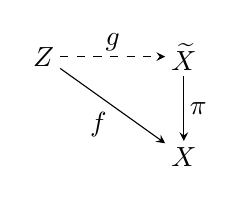
\begin{tikzpicture}[x=1.78cm,y=1.27cm,every node/.style={inner sep=2pt},>=stealth]
\node (z) at (0,0) {$Z$};
\node (xt) at (1,0) {$\widetilde X$};
\node (x) at (1,-1) {$X$};
\draw[->,dashed] (z) -- node[above] {$g$} (xt);
\draw[->] (xt) -- node[right] {$\pi$} (x);
\draw[->] (z) -- node[below left] {$f$} (x);
\end{tikzpicture}
\]

\smallskip
\noindent\textsc{Proof.} In view of the asserted uniqueness of $g$, the question is local on $X$. So we may assume that $X=\operatorname{Spec}A$ is affine, $A$ is noetherian, and that $\mathcal I$ corresponds to an ideal $I\subseteq A$. Then $\widetilde X=\operatorname{Proj}S$, where $S=\bigoplus_{d\geq0}I^d$. Let $a_0,\ldots,a_n\in I$ be a set of generators for the ideal $I$. Then we can define a surjective map of graded rings $\varphi\colon A[x_0,\ldots,x_n]\to S$ by sending $x_i$ to $a_i\in I$, considered as an element of degree one in $S$. This homomorphism gives rise to a closed immersion $\widetilde X\hookrightarrow\Proj_A^n$. The kernel of $\varphi$ is the homogeneous ideal in $A[x_0,\ldots,x_n]$ generated by all homogeneous polynomials $F(x_0,\ldots,x_n)$ such that $F(a_0,\ldots,a_n)=0$ in $A$.

Now let $f\colon Z\to X$ be a morphism such that the inverse image ideal sheaf $f^{-1}\mathcal I\cdot\mathcal O_Z$ is an invertible sheaf $\mathcal L$ on $Z$. Since $I$ is generated by $a_0,\ldots,a_n$, the inverse images of these elements, considered as global sections of $\mathcal I$, give global sections $s_0,\ldots,s_n$ of $\mathcal L$ which generate. Then by \Goto{result-II-7.1}{(7.1)} there is a unique
}
% Contents from body/page-179.tex.
\ChapterSheet{179}{165}{\Goto{sec-II-7}{7\quad Projective Morphisms}}{%
morphism $g\colon Z\to\Proj_A^n$ with the property that $\mathcal L\cong g^*\mathcal O(1)$ and that \EditionText{$s_i=g^*x_i$} under this isomorphism. Now I claim that $g$ factors through the closed subscheme $\widetilde X$ of $\Proj_A^n$. This follows easily from the fact that if $F(x_0,\ldots,x_n)$ is a homogeneous element of degree $d$ of $\ker\varphi$, where $\ker\varphi$ is the homogeneous ideal described above which determines $\widetilde X$, then $F(a_0,\ldots,a_n)=0$ in $A$ and so $F(s_0,\ldots,s_n)=0$ in $\Gamma(Z,\mathcal L^d)$.

Thus we have constructed a morphism $g\colon Z\to\widetilde X$ factoring $f$. For any such morphism, we must necessarily have $f^{-1}\mathcal I\cdot\mathcal O_Z=g^{-1}(\pi^{-1}\mathcal I\cdot\mathcal O_{\widetilde X})\cdot\mathcal O_Z$ which is just $g^{-1}(\mathcal O_{\widetilde X}(1))\cdot\mathcal O_Z$. Therefore we have a surjective map $g^*\mathcal O_{\widetilde X}(1)\to f^{-1}\mathcal I\cdot\mathcal O_Z=\mathcal L$. Now a surjective map of invertible sheaves on a locally ringed space is necessarily an isomorphism (Ex.~\Goto{ex-II-7.1}{7.1}), so we have $g^*\mathcal O_{\widetilde X}(1)\cong\mathcal L$. Clearly the sections $s_i$ of $\mathcal L$ must be the pull-backs of the sections $x_i$ of $\mathcal O(1)$ on $\Proj_A^n$. Hence the uniqueness of $g$ under our conditions follows from the uniqueness assertion of \Goto{result-II-7.1}{(7.1)}.

\medskip
\noindent\hypertarget{result-II-7.15}{}\textbf{Corollary 7.15.} \emph{Let $f\colon Y\to X$ be a morphism of noetherian schemes, and let $\mathcal I$ be a coherent sheaf of ideals on $X$. Let $\widetilde X$ be the blowing-up of $\mathcal I$, and let $\widetilde Y$ be the blowing-up of the inverse image ideal sheaf $\mathcal J=f^{-1}\mathcal I\cdot\mathcal O_Y$ on $Y$. Then there is a unique morphism $\widetilde f\colon\widetilde Y\to\widetilde X$}
\[
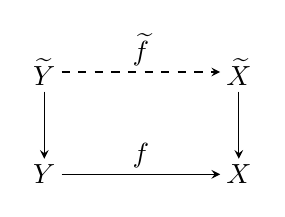
\begin{tikzpicture}[x=2.47cm,y=1.30cm,every node/.style={inner sep=2pt},>=stealth]
\node (yt) at (0,0) {$\widetilde Y$};
\node (xt) at (1,0) {$\widetilde X$};
\node (y) at (0,-1) {$Y$};
\node (x) at (1,-1) {$X$};
\draw[->,dashed] (yt) -- node[above] {$\widetilde f$} (xt);
\draw[->] (yt) -- (y);
\draw[->] (xt) -- (x);
\draw[->] (y) -- node[above] {$f$} (x);
\end{tikzpicture}
\]
\emph{making a commutative diagram as shown. Moreover, if $f$ is a closed immersion, so is $\widetilde f$.}

\smallskip
\noindent\textsc{Proof.} The existence and uniqueness of $\widetilde f$ follow immediately from the proposition. To show that $\widetilde f$ is a closed immersion if $f$ is, we go back to the definition of blowing up. $\widetilde X=\operatorname{\mathbf{Proj}}\mathcal S$ where $\mathcal S=\bigoplus_{d\geq0}\mathcal I^d$, and $\widetilde Y=\operatorname{\mathbf{Proj}}\mathcal S'$, where $\mathcal S'=\bigoplus_{d\geq0}\mathcal J^d$. Since $Y$ is a closed subscheme of $X$, we can consider $\mathcal S'$ as a sheaf of graded algebras on $X$. Then there is a natural surjective homomorphism of graded rings $\mathcal S\to\mathcal S'$, which gives rise to the closed immersion $\widetilde f$.

\medskip
\noindent\textbf{Definition.} In the situation of \Goto{result-II-7.15}{(7.15)}, if $Y$ is a closed subscheme of $X$, we call the closed subscheme $\widetilde Y$ of $\widetilde X$ the \emph{strict transform} of $Y$ under the blowing-up $\pi\colon\widetilde X\to X$.

\medskip
\noindent\hypertarget{result-II-7.15.1}{}\textbf{Example 7.15.1.} If $Y$ is a closed subvariety of $X=\AffSpace[k]{n}$ passing through the origin $P$\EditionText{ with $Y\ne\{P\}$}, then the strict transform $\widetilde Y$ of $Y$ in $\widetilde X$ is a closed subvariety. Hence\EditionText{} we can recover $\widetilde Y$ as the closure of $\pi^{-1}(Y-P)$,
}
% Contents from body/page-180.tex.
\usetikzlibrary{arrows}
\ChapterSheet{180}{166}{\Goto{p-74}{II\quad Schemes}}{%
where $\pi\colon\pi^{-1}(X-P)\to X-P$ is the isomorphism of \Goto{result-II-7.13b}{(7.13b)}. This shows that our new definition of blowing up coincides with the one given in (I, \Goto{sec-I-4}{\S4}) for any closed subvariety of $\AffSpace[k]{n}$. In particular, this shows that blowing up as defined earlier is intrinsic.

\medskip
Now we will study blowing up in the special case that $X$ is a variety. Recall (\Goto{sec-II-4}{\S4}) that a variety is defined to be an integral separated scheme of finite type over an algebraically closed field $k$.

\medskip
\noindent\hypertarget{result-II-7.16}{}\textbf{Proposition 7.16.} \emph{Let $X$ be a variety over $k$, let $\mathcal I\subseteq\mathcal O_X$ be a nonzero coherent sheaf of ideals on $X$, and let $\pi\colon\widetilde X\to X$ be the blowing-up with respect to $\mathcal I$. Then:}
\par{\itshape\leftskip=12pt
\hypertarget{result-II-7.16a}{}(a) $\widetilde X$ is also a variety;

\hypertarget{result-II-7.16b}{}(b) $\pi$ is a birational, proper, surjective morphism;

\hypertarget{result-II-7.16c}{}(c) if $X$ is quasi-projective (respectively, projective) over $k$, then $\widetilde X$ is also, and $\pi$ is a projective morphism.\par}

\smallskip
\noindent\textsc{Proof.} First of all, since $X$ is integral, the sheaf $\mathcal S=\bigoplus_{d\geq0}\mathcal I^d$ is a sheaf of integral domains on $X$, so $\widetilde X$ is also integral. Next, we have already seen that $\pi$ is proper \Goto{result-II-7.10}{(7.10)}. In particular, $\pi$ is separated and of finite type, so it follows that $\widetilde X$ is also separated and of finite type, i.e., $\widetilde X$ is a variety. Now since $\mathcal I\ne0$, the corresponding closed subscheme $Y$ is not all of $X$, and so the open set $U=X-Y$ is nonempty. Since $\pi$ induces an isomorphism from $\pi^{-1}U$ to $U$ \Goto{result-II-7.13}{(7.13)}, we see that $\pi$ is birational. Since $\pi$ is proper, it is a closed map, so the image $\pi(\widetilde X)$ is a closed set containing $U$, which must be all of $X$ since $X$ is irreducible. Thus $\pi$ is surjective. Finally, if $X$ is quasi-projective (respectively, projective), then $X$ admits an ample invertible sheaf \Goto{result-II-7.6}{(7.6)}, so by \Goto{result-II-7.10b}{(7.10b)} $\pi$ is a projective morphism. It follows that $\widetilde X$ is also quasi-projective (respectively, projective) (Ex.~\Goto{ex-II-4.9}{4.9}).

\medskip
\noindent\hypertarget{result-II-7.17}{}\textbf{Theorem 7.17.} \emph{Let $X$ be a quasi-projective variety over $k$. If $Z$ is another variety and $f\colon Z\to X$ is any birational projective morphism, then there exists a coherent sheaf of ideals $\mathcal I$ on $X$ such that $Z$ is isomorphic to the blowing-up $\widetilde X$ of $X$ with respect to $\mathcal I$, and $f$ corresponds to $\pi\colon\widetilde X\to X$ under this isomorphism.}

\smallskip
\noindent\textsc{Proof.} The proof is somewhat difficult, so we divide it into steps.

\hypertarget{step-II-7.17-1}{}\emph{Step 1.} Since $f$ is assumed to be a projective morphism, there exists a closed immersion $i\colon Z\to\Proj_X^n$ for some $n$.
\[
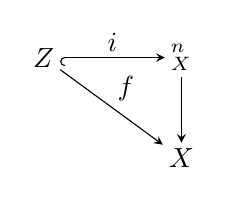
\begin{tikzpicture}[x=1.75cm,y=1.28cm,every node/.style={inner sep=2pt},>=stealth]
\node (z) at (0,0) {$Z$};
\node (p) at (1,0) {$\Proj_X^n$};
\node (x) at (1,-1) {$X$};
\draw[left hook-stealth] (z) -- node[above] {$i$} (p);
\draw[->] (p) -- (x);
\draw[->] (z) -- node[above right] {$f$} (x);
\end{tikzpicture}
\]
}
% Contents from body/page-181.tex.
\ChapterSheet{181}{167}{\Goto{sec-II-7}{7\quad Projective Morphisms}}{%
Let $\mathcal L$ be the invertible sheaf $i^*\mathcal O(1)$ on $Z$. Now we consider the sheaf of graded $\mathcal O_X$-algebras $\mathcal S=\mathcal O_X\oplus\bigoplus_{d\geq1}f_*\mathcal L^d$. Each $f_*\mathcal L^d$ is a coherent sheaf on $X$, by \Goto{result-II-5.20}{(5.20)}, so $\mathcal S$ is quasi-coherent. However, $\mathcal S$ may not be generated by $\mathcal S_1$ as an $\mathcal O_X$-algebra.

\hypertarget{step-II-7.17-2}{}\emph{Step 2.} For any integer $e>0$, let $\mathcal S^{(e)}=\bigoplus_{d\geq0}\mathcal S_d^{(e)}$, where $\mathcal S_d^{(e)}=\mathcal S_{de}$ (cf. Ex.~\Goto{ex-II-5.13}{5.13}). I claim that for $e$ sufficiently large, $\mathcal S^{(e)}$ is generated as an $\mathcal O_X$-algebra by $\mathcal S_1^{(e)}$. Since $X$ is quasi-compact, this question is local on $X$, so we may assume $X=\operatorname{Spec}A$ is affine, where $A$ is a finitely generated $k$-algebra. Then $Z$ is a closed subscheme of $\Proj_A^n$, and $\mathcal S$ corresponds to the graded $A$-algebra $S=A\oplus\bigoplus_{d\geq1}\Gamma(Z,\mathcal O_Z(d))$. Let $T=A[x_0,\ldots,x_n]/I_Z$, where $I_Z$ is a homogeneous ideal defining $Z$. Then, using the technique of (Ex.~\Goto{ex-II-5.9}{5.9}, Ex.~\Goto{ex-II-5.14}{5.14}), one can show that the $A$-algebras $S,T$ agree in all large enough degrees (details left to reader). But $T$ is generated as an $A$-algebra by $T_1$, so $T^{(e)}$ is generated by $T_1^{(e)}$, and this is the same as $S^{(e)}$ for $e$ sufficiently large.

\hypertarget{step-II-7.17-3}{}\emph{Step 3.} Now let us replace our original embedding $i\colon Z\to\Proj_X^n$ by $i$ followed by an $e$-uple embedding for $e$ sufficiently large. This has the effect of replacing $\mathcal L$ by $\mathcal L^e$ and $\mathcal S$ by $\mathcal S^{(e)}$ (Ex.~\Goto{ex-II-5.13}{5.13}). Thus we may now assume that $\mathcal S$ is generated by $\mathcal S_1$ as an $\mathcal O_X$-algebra. Note also by construction that $Z\cong\operatorname{\mathbf{Proj}}\mathcal S$ (cf.~\Goto{result-II-5.16}{(5.16)}). So at least we have $Z$ isomorphic to \textbf{Proj} of something. If $\mathcal S_1=f_*\mathcal L$ were a sheaf of ideals in $\mathcal O_X$ we would be done. So in the next step, we try to make it into one.

\hypertarget{step-II-7.17-4}{}\emph{Step 4.} Now $\mathcal L$ is an invertible sheaf on the integral scheme $Z$, so we can find an embedding $\mathcal L\hookrightarrow\mathcal K_Z$ where $\mathcal K_Z$ is the constant sheaf of the function field of $Z$ (proof of \Goto{result-II-6.15}{6.15}). Hence $f_*\mathcal L\subseteq f_*\mathcal K_Z$. But since $f$ is assumed to be birational, we have $f_*\mathcal K_Z=\mathcal K_X$, and so $f_*\mathcal L\subseteq\mathcal K_X$. Now let $\mathcal M$ be an ample invertible sheaf on $X$, which exists because $X$ is assumed to be quasi-projective. Then I claim that there is an $n>0$ and an embedding $\mathcal M^{-n}\subseteq\mathcal K_X$ such that $\mathcal M^{-n}\cdot f_*\mathcal L\subseteq\mathcal O_X$. Indeed, let $\mathcal J$ be the \emph{ideal sheaf of denominators} of $f_*\mathcal L$, defined locally as $\{a\in\mathcal O_X\mid a\cdot f_*\mathcal L\subseteq\mathcal O_X\}$. This is a nonzero coherent sheaf of ideals on $X$, because $f_*\mathcal L$ is a coherent subsheaf of $\mathcal K_X$, so locally one can just take common denominators for a set of generators of the corresponding finitely generated module. Since $\mathcal M$ is ample, $\mathcal J\otimes\mathcal M^n$ is generated by global sections for $n$ sufficiently large. In particular, for suitable $n>0$, there is a nonzero map $\mathcal O_X\to\mathcal J\otimes\mathcal M^n$, and hence a nonzero map $\mathcal M^{-n}\to\mathcal J$. Then by construction $\mathcal M^{-n}\cdot f_*\mathcal L\subseteq\mathcal O_X$.

\hypertarget{step-II-7.17-5}{}\emph{Step 5.} Since $\mathcal M^{-n}\cdot f_*\mathcal L\subseteq\mathcal O_X$, it is a coherent sheaf of ideals on $X$, which we call $\mathcal I$. This is the required ideal sheaf, as we will now show that $Z$ is isomorphic to the blowing up of $X$ with respect to $\mathcal I$. We already know that $Z\cong\operatorname{\mathbf{Proj}}\mathcal S$. Therefore by \Goto{result-II-7.9}{(7.9)} $Z$ is also isomorphic to $\operatorname{\mathbf{Proj}}\mathcal S*\mathcal M^{-n}$. So to complete the proof, it will be sufficient to identify $(\mathcal S*\mathcal M^{-n})_d=\mathcal M^{-dn}\otimes f_*\mathcal L^d$ with $\mathcal I^d$ for any $d\geq1$. First note that $f_*\mathcal L^d\subseteq\mathcal K_X$ for any $d$ (same reason as above for $d=1$), and since $\mathcal M$ is invertible, we can write $\mathcal M^{-dn}\cdot f_*\mathcal L^d$ instead of $\otimes$. Now since $\mathcal S$ is locally generated by $\mathcal S_1$ as an $\mathcal O_X$-algebra, we have a natural surjective map $\mathcal I^d\to\mathcal M^{-dn}\cdot f_*\mathcal L^d$ for each
}
% Contents from body/page-182.tex.
\usetikzlibrary{arrows}
\ChapterSheet{182}{168}{\Goto{p-74}{II\quad Schemes}}{%
$d\geq1$. It must also be injective, since both are subsheaves of $\mathcal K_X$, so it is an isomorphism. This shows finally that $Z\cong\operatorname{\mathbf{Proj}}\bigoplus_{d\geq0}\mathcal I^d$, which completes the proof.

\medskip
\noindent\hypertarget{result-II-7.17.1}{}\textbf{Remark 7.17.1.} Of course the sheaf of ideals $\mathcal I$ in the theorem is not unique. This is clear from the construction, but see also (Ex.~\Goto{ex-II-7.11}{7.11}).

\medskip
\noindent\hypertarget{result-II-7.17.2}{}\textbf{Remark 7.17.2.} We see from this theorem that blowing up arbitrary coherent sheaves of ideals is a very general process. Accordingly in most applications one learns more by blowing up only along some restricted class of subvarieties. For example, in his paper on resolution of singularities \Goto{bib-hironaka-4}{[4]}, Hironaka uses only blowing up along a nonsingular subvariety which is \textquotedblleft{}normally flat\textquotedblright{} in its ambient space. In studying birational geometry of surfaces in Chapter \Goto{p-370}{V}, we will use only blowing up at a point. In fact one of our main results there will be that any birational transformation of nonsingular projective surfaces can be factored into a finite number of blowings up (and blowings down) of points. One important application of the more general blowing-up we have been studying here is Nagata's theorem \Goto{bib-nagata-6}{[6]} that any (abstract) variety can be embedded as an open subset of a complete variety.

\medskip
\noindent\hypertarget{result-II-7.17.3}{}\textbf{Example 7.17.3.} As an example of the general concept of blowing up a coherent sheaf of ideals, we show how to eliminate the points of indeterminacy of a rational map determined by an invertible sheaf. So let $A$ be a ring, let $X$ be a noetherian scheme over $A$, let $\mathcal L$ be an invertible sheaf on $X$, and let $s_0,\ldots,s_n\in\Gamma(X,\mathcal L)$ be a set of global sections of $\mathcal L$. Let $U$ be the open subset of $X$ where the $s_i$ generate the sheaf $\mathcal L$. Then according to \Goto{result-II-7.1}{(7.1)} the invertible sheaf $\mathcal L|_U$ on $U$ and the global sections $s_0,\ldots,s_n$ determine an $A$-morphism $\varphi\colon U\to\Proj_A^n$. We will now show how to blow up a certain sheaf of ideals $\mathcal I$ on $X$, whose corresponding closed subscheme $Y$ has support equal to $X-U$ (i.e., the underlying topological space of $Y$ is $X-U$), so that the morphism $\varphi$ extends to a morphism $\widetilde\varphi$ of $\widetilde X$ to $\Proj_A^n$.
\[
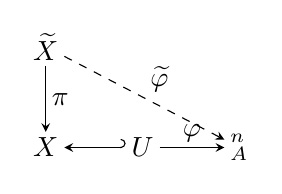
\begin{tikzpicture}[x=1.23cm,y=1.28cm,every node/.style={inner sep=2pt},>=stealth]
\node (xt) at (0,0) {$\widetilde X$};
\node (x) at (0,-1) {$X$};
\node (u) at (1,-1) {$U$};
\node (p) at (2,-1) {$\Proj_A^n$};
\draw[->] (xt) -- node[right] {$\pi$} (x);
\draw[left hook-stealth] (u) -- (x);
\draw[->] (u) -- node[above] {$\varphi$} (p);
\draw[->,dashed] (xt) -- node[above right] {$\widetilde\varphi$} (p);
\end{tikzpicture}
\]

So let $\mathcal F$ be the coherent subsheaf of $\mathcal L$ generated by $s_0,\ldots,s_n$. We define a coherent sheaf of ideals $\mathcal I$ on $X$ as follows: for any open set $V\subseteq X$, such that $\mathcal L|_V$ is free, let $\psi\colon\mathcal L|_V\xrightarrow{\sim}\mathcal O_V$ be an isomorphism, and take $\mathcal I|_V=\psi(\mathcal F|_V)$. Clearly the ideal sheaf $\mathcal I|_V$ is independent of the choice of $\psi$, so we get a well-defined coherent sheaf of ideals $\mathcal I$ on $X$. Note also that $\mathcal I_x=\mathcal O_x$ if and~only
}
% Contents from body/page-183.tex.
\ChapterSheet{183}{169}{\Goto{sec-II-7}{7\quad Projective Morphisms}}{%
\noindent if $x\in U$, so the corresponding closed subscheme $Y$ has support equal to $X-U$. Let $\pi\colon\widetilde X\to X$ be the blowing-up of $\mathcal I$. Then by (\Goto{result-II-7.13}{7.13a}), $\pi^{-1}\mathcal I\cdot\mathcal O_{\widetilde X}$ is an invertible sheaf of ideals, so we see that the global sections $\pi^*s_i$ of $\pi^*\mathcal L$ generate an \emph{invertible} coherent subsheaf $\mathcal L'$ of $\pi^*\mathcal L$. Now $\mathcal L'$ and the sections $\pi^*s_i$ define a morphism $\widetilde\varphi\colon\widetilde X\to\Proj_A^n$ whose restriction to $\pi^{-1}(U)$ corresponds to $\varphi$ under the natural isomorphism $\pi\colon\pi^{-1}(U)\xrightarrow{\sim}U$ (\Goto{result-II-7.13}{7.13b}).

In case $X$ is a nonsingular projective variety over a field, we can rephrase this example in terms of linear systems. The given $\mathcal L$ and sections $s_i$ determine a linear system $\mathfrak d$ on $X$. The base points of $\mathfrak d$ are just the points of the closed set $X-U$, and $\varphi\colon U\to\Proj_k^n$ is the morphism determined by the base-point-free linear system $\mathfrak d|_U$ on $U$. We call $Y$ the \emph{scheme} of base points of $\mathfrak d$. So our example shows that if we blow up $Y$, then $\mathfrak d$ extends to a base-point-free linear system $\widetilde{\mathfrak d}$ on all of $\widetilde X$.

\Exercises
{\fontsize{9}{10.5}\selectfont
\begin{description}[style=multiline,labelwidth=1.8em,leftmargin=2.1em,itemsep=4pt,topsep=2pt,parsep=0pt]
\item[\hypertarget{ex-II-7.1}{}7.1.] Let $(X,\mathcal O_X)$ be a locally ringed space, and let $f\colon\mathcal L\to\mathcal M$ be a surjective map of invertible sheaves on $X$. Show that $f$ is an isomorphism. [\emph{Hint:} Reduce to a question of modules over a local ring by looking at the stalks.]
\item[\hypertarget{ex-II-7.2}{}7.2.] Let $X$ be a scheme over a field $k$. Let $\mathcal L$ be an invertible sheaf on $X$, and let $\{s_0,\ldots,s_n\}$ and $\{t_0,\ldots,t_m\}$ be two sets of sections of $\mathcal L$, which generate the same subspace $V\subseteq\Gamma(X,\mathcal L)$, and which generate the sheaf $\mathcal L$ at every point. Suppose $n\le m$. Show that the corresponding morphisms $\varphi\colon X\to\Proj_k^n$ and $\psi\colon X\to\Proj_k^m$ differ by a suitable linear projection $\Proj^m-L\to\Proj^n$ and an automorphism of $\Proj^n$, where $L$ is a linear subspace of $\Proj^m$ of dimension $m-n-1$.
\item[\hypertarget{ex-II-7.3}{}7.3.] Let $\varphi\colon\Proj_k^n\to\Proj_k^m$ be a morphism. Then:
\begin{parts}
\item either $\varphi(\Proj^n)=pt$ or $m\ge n$ and $\dim\varphi(\Proj^n)=n$;
\item in the second case, $\varphi$ can be obtained as the composition of \hypertarget{cond-II-7.3-1}{}(1) a $d$-uple embedding $\Proj^n\to\Proj^N$ for a uniquely determined $d\ge 1$, \hypertarget{cond-II-7.3-2}{}(2) a linear projection $\Proj^N-L\to\Proj^m$, and \hypertarget{cond-II-7.3-3}{}(3) an automorphism of $\Proj^m$. Also, $\varphi$ has finite fibres.
\end{parts}
\item[\hypertarget{ex-II-7.4}{}7.4.]
\begin{parts}
\item[\hypertarget{ex-II-7.4a}{}(a)] Use (\Goto{result-II-7.6}{7.6}) to show that if $X$ is a scheme of finite type over a noetherian ring $A$, and if $X$ admits an ample invertible sheaf, then $X$ is separated.
\item Let $X$ be the affine line over a field $k$ with the origin doubled (\Goto{result-II-4.0.1}{4.0.1}). Calculate $\operatorname{Pic} X$, determine which invertible sheaves are generated by global sections, and then show directly (without using (\Goto{ex-II-7.4a}{a})) that there is no ample invertible sheaf on $X$.
\end{parts}
\item[\hypertarget{ex-II-7.5}{}7.5.] Establish the following properties of ample and very ample invertible sheaves on a noetherian scheme $X$. $\mathcal L,\mathcal M$ will denote invertible sheaves, and for (\Goto{ex-II-7.5d}{d}), (\Goto{ex-II-7.5e}{e}) we assume furthermore that $X$ is of finite type over a noetherian ring $A$.
\begin{parts}
\item[\hypertarget{ex-II-7.5a}{}(a)] If $\mathcal L$ is ample and $\mathcal M$ is generated by global sections, then $\mathcal L\otimes\mathcal M$ is ample.
\item[\hypertarget{ex-II-7.5b}{}(b)] If $\mathcal L$ is ample and $\mathcal M$ is arbitrary, then $\mathcal M\otimes\mathcal L^n$ is ample for sufficiently large $n$.
\item[\hypertarget{ex-II-7.5c}{}(c)] If $\mathcal L,\mathcal M$ are both ample, so is $\mathcal L\otimes\mathcal M$.
\item[\hypertarget{ex-II-7.5d}{}(d)] If $\mathcal L$ is very ample and $\mathcal M$ is generated by global sections, then $\mathcal L\otimes\mathcal M$ is very ample.
\item[\hypertarget{ex-II-7.5e}{}(e)] If $\mathcal L$ is ample, then there is an $n_0>0$ such that $\mathcal L^n$ is very ample for all $n\ge n_0$.
\end{parts}
\end{description}
}
}
% Contents from body/page-184.tex.
\ChapterSheet{184}{170}{\Goto{p-74}{II\quad Schemes}}{%
{\fontsize{8.8}{9.5}\selectfont\setlength{\parskip}{0pt}
\begin{description}[style=multiline,labelwidth=2.6em,leftmargin=2.9em,itemsep=2pt,topsep=0pt,parsep=0pt]
\item[\hypertarget{ex-II-7.6}{}7.6.] \emph{The Riemann--Roch Problem.} Let $X$ be a nonsingular projective variety over an algebraically closed field, and let $D$ be a divisor on $X$. For any $n>0$ we consider the complete linear system $|nD|$. Then the Riemann--Roch problem is to determine $\dim|nD|$ as a function of $n$, and, in particular, its behavior for large $n$. If $\mathcal L$ is the corresponding invertible sheaf, then $\dim|nD|=\dim\Gamma(X,\mathcal L^n)-1$, so an equivalent problem is to determine $\dim\Gamma(X,\mathcal L^n)$ as a function of $n$.
\begin{enumerate}[label=\normalfont(\alph*),leftmargin=1.48em,itemsep=0pt,topsep=0pt,parsep=0pt]
\item Show that if $D$ is very ample, and if $X\hookrightarrow\Proj_k^N$ is the corresponding embedding in projective space, then for all $n$ sufficiently large, $\dim|nD|=P_X(n)-1$, where $P_X$ is the \emph{Hilbert polynomial} of $X$ (I, \S\Goto{sec-I-7}{7}). Thus in this case $\dim|nD|$ is a polynomial function of $n$, for $n$ large.
\item If $D$ corresponds to a torsion element of $\operatorname{Pic} X$, of order $r$, then $\dim|nD|=0$ if $r\mid n$, $-1$ otherwise. In this case the function is periodic of period $r$.
\end{enumerate}
\hspace{1em}It follows from the general Riemann--Roch theorem that $\dim|nD|$ is a polynomial function for $n$ large, whenever $D$ is an \emph{ample} divisor. See (IV, \Goto{result-IV-1.3.2}{1.3.2}), (V, \Goto{result-V-1.6}{1.6}), and Appendix~\Goto{p-438}{A}. In the case of algebraic surfaces, Zariski \Goto{bib-483-18}{[7]} has shown for any effective divisor $D$, that there is a finite set of polynomials $P_1,\ldots,P_r$, such that for all $n$ sufficiently large, $\dim|nD|=P_{i(n)}(n)$, where $i(n)\in\{1,2,\ldots,r\}$ is a function of $n$.
\item[\hypertarget{ex-II-7.7}{}7.7.] \emph{Some Rational Surfaces.} Let $X=\Proj_k^2$, and let $|D|$ be the complete linear system of all divisors of degree $2$ on $X$ (conics). $D$ corresponds to the invertible sheaf $\mathcal O(2)$, whose space of global sections has a basis $x^2,y^2,z^2,xy,xz,yz$, where $x,y,z$ are the homogeneous coordinates of $X$.
\begin{enumerate}[label=\normalfont(\alph*),leftmargin=1.48em,itemsep=0pt,topsep=0pt,parsep=0pt]
\item The complete linear system $|D|$ gives an embedding of $\Proj^2$ in $\Proj^5$, whose image is the Veronese surface (I, Ex.~\Goto{ex-I-2.13}{2.13}).
\item \EditionText{Assume $\operatorname{char}k\ne 2$. Show} that the subsystem defined by $x^2,y^2,z^2,y(x-z),(x-y)z$ gives a closed immersion of $X$ into $\Proj^4$. The image is called the \emph{Veronese surface in $\Proj^4$}. Cf. (IV, Ex.~\Goto{ex-IV-3.11}{3.11}).
\item Let $\mathfrak d\subseteq|D|$ be the linear system of all conics passing through a fixed point $P$. Then $\mathfrak d$ gives an immersion of $U=X-P$ into $\Proj^4$. Furthermore, if we blow up $P$, to get a surface $\widetilde X$, then this map extends to give a closed immersion of $\widetilde X$ in $\Proj^4$. Show that $\widetilde X$ is a surface of degree $3$ in $\Proj^4$, and that the lines in $X$ through $P$ are transformed into straight lines in $\widetilde X$ which do not meet. $\widetilde X$ is the union of all these lines, so we say $\widetilde X$ is a \emph{ruled surface} (V, \Goto{result-V-2.19.1}{2.19.1}).
\end{enumerate}
\item[\hypertarget{ex-II-7.8}{}7.8.] Let $X$ be a noetherian scheme, let $\mathcal E$ be a coherent locally free sheaf on $X$, and let $\pi\colon\Proj(\mathcal E)\to X$ be the corresponding projective space bundle. Show that there is a natural 1-1 correspondence between \emph{sections} of $\pi$ (i.e., morphisms $\sigma\colon X\to\Proj(\mathcal E)$ such that $\pi\circ\sigma=\operatorname{id}_X$) and quotient invertible sheaves $\mathcal E\to\mathcal L\to 0$ of $\mathcal E$.
\item[\hypertarget{ex-II-7.9}{}7.9.] Let $X$ be a regular noetherian scheme, and $\mathcal E$ a locally free coherent sheaf of rank $\ge 2$ on $X$.
\begin{enumerate}[label=\normalfont(\alph*),leftmargin=1.48em,itemsep=0pt,topsep=0pt,parsep=0pt]
\item \EditionText{If $X$ is connected, show that $\operatorname{Pic}\Proj(\mathcal E)\cong\operatorname{Pic}X\times\mathbb Z$. For arbitrary $X$, replace $\mathbb Z$ by the group of locally constant integer-valued functions on $X$.}
\item If $\mathcal E'$ is another locally free coherent sheaf on $X$, show that $\Proj(\mathcal E)\cong\Proj(\mathcal E')$ (over $X$) if and only if there is an invertible sheaf $\mathcal L$ on $X$ such that $\mathcal E'\cong\mathcal E\otimes\mathcal L$.
\end{enumerate}
\item[\hypertarget{ex-II-7.10}{}7.10.] \emph{$\Proj^n$-Bundles Over a Scheme.} Let $X$ be a noetherian scheme.
\begin{enumerate}[label=\normalfont(\alph*),leftmargin=1.48em,itemsep=0pt,topsep=0pt,parsep=0pt]
\item By analogy with the definition of a vector bundle (Ex.~\Goto{ex-II-5.18}{5.18}), define the notion of a \emph{projective $n$-space bundle} over $X$, as a scheme $P$ with a morphism $\pi\colon P\to X$ such that $P$ is locally isomorphic to $U\times\Proj^n$, $U\subseteq X$ open, and the transition automorphisms on $\operatorname{Spec}A\times\Proj^n$ are given by $A$-linear automorphisms of the homogeneous coordinate ring $A[x_0,\ldots,x_n]$ (e.g., $x_i'=\sum a_{ij}x_j$, $a_{ij}\in A$).
\item If $\mathcal E$ is a locally free sheaf of rank $n+1$ on $X$, then $\Proj(\mathcal E)$ is a $\Proj^n$-bundle over $X$.
\end{enumerate}
\end{description}
}
}
% Contents from body/page-185.tex.
\ChapterSheet{185}{171}{\Goto{sec-II-7}{7\quad Projective Morphisms}}{%
{\fontsize{9}{10.1}\selectfont\setlength{\parskip}{0pt}
\begin{description}[style=multiline,labelwidth=3.15em,leftmargin=3.45em,itemsep=3pt,topsep=0pt,parsep=0pt]
\item[]
\begin{parts}
\item[*(c)] Assume that $X$ is regular, and show that every $\Proj^n$-bundle $P$ over $X$ is isomorphic to $\Proj(\mathcal E)$ for some locally free sheaf $\mathcal E$ on $X$. [\emph{Hint:} Let $U\subseteq X$ be an open set such that $\pi^{-1}(U)\cong U\times\Proj^n$, and let $\mathcal L_0$ be the invertible sheaf $\mathcal O(1)$ on $U\times\Proj^n$. Show that $\mathcal L_0$ extends to an invertible sheaf $\mathcal L$ on $P$. Then show that $\pi_*\mathcal L=\mathcal E$ is a locally free sheaf on $X$ and that $P\cong\Proj(\mathcal E)$.] Can you weaken the hypothesis \textquotedblleft{}$X$ regular\textquotedblright{}?
\item[(d)] Conclude (in the case $X$ regular) that we have a 1-1 correspondence between $\Proj^n$-bundles over $X$, and equivalence classes of locally free sheaves $\mathcal E$ of rank $n+1$ under the equivalence relation $\mathcal E'\sim\mathcal E$ if and only if $\mathcal E'\cong\mathcal E\otimes\mathcal M$ for some invertible sheaf $\mathcal M$ on $X$.
\end{parts}
\item[\hypertarget{ex-II-7.11}{}7.11.] On a noetherian scheme $X$, different sheaves of ideals can give rise to isomorphic blown up schemes.
\begin{parts}
\item If $\mathcal I$ is any coherent sheaf of ideals on $X$, show that blowing up $\mathcal I^d$ for any $d\ge1$ gives a scheme isomorphic to the blowing up of $\mathcal I$ (cf. Ex.~\Goto{ex-II-5.13}{5.13}).
\item If $\mathcal I$ is any coherent sheaf of ideals, and if $\mathcal J$ is an invertible sheaf of ideals, then $\mathcal I$ and $\mathcal I\cdot\mathcal J$ give isomorphic blowings-up.
\item If $X$ is regular, show that (\Goto{result-II-7.17}{7.17}) can be strengthened as follows. Let $U\subseteq X$ be the largest open set such that $f\colon f^{-1}U\to U$ is an isomorphism. Then $\mathcal I$ can be chosen such that the corresponding closed subscheme $Y$ has support equal to $X-U$.
\end{parts}
\item[\hypertarget{ex-II-7.12}{}7.12.] Let $X$ be a noetherian scheme, and let $Y,Z$ be two closed subschemes, neither one containing the other. Let $\widetilde X$ be obtained by blowing up $Y\cap Z$ (defined by the ideal sheaf $\mathcal I_Y+\mathcal I_Z$). Show that the strict transforms $\widetilde Y$ and $\widetilde Z$ of $Y$ and $Z$ in $\widetilde X$ do not meet.
\item[\hypertarget{ex-II-7.13}{}*7.13.] \emph{A Complete Nonprojective Variety.} Let $k$ be an algebraically closed field of $\operatorname{char}\ne2$. Let $C\subseteq\Proj_k^2$ be the nodal cubic curve $y^2z=x^3+x^2z$. If $P_0=(0,0,1)$ is the singular point, then $C-P_0$ is isomorphic to the multiplicative group $\mathbf G_m=\operatorname{Spec}k[t,t^{-1}]$ (Ex.~\Goto{ex-II-6.7}{6.7}). For each $a\in k$, $a\ne0$, consider the translation of $\mathbf G_m$ given by $t\mapsto at$. This induces an automorphism of $C$ which we denote by $\varphi_a$.

\hspace{1em}Now consider $C\times(\Proj^1-\{0\})$ and $C\times(\Proj^1-\{\infty\})$. We glue their open subsets $C\times(\Proj^1-\{0,\infty\})$ by the isomorphism $\varphi\colon\langle P,u\rangle\mapsto\langle\varphi_u(P),u\rangle$ for $P\in C$, $u\in\mathbf G_m=\Proj^1-\{0,\infty\}$. Thus we obtain a scheme $X$, which is our example. The projections to the second factor are compatible with $\varphi$, so there is a natural morphism $\pi\colon X\to\Proj^1$.
\begin{parts}
\item Show that $\pi$ is a proper morphism, and hence that $X$ is a complete variety over $k$.
\item Use the method of (Ex.~\Goto{ex-II-6.9}{6.9}) to show that $\operatorname{Pic}(C\times\AffSpace{1})\cong\mathbf G_m\times\mathbb Z$ and $\operatorname{Pic}(C\times(\AffSpace{1}-\{0\}))\cong\mathbf G_m\times\mathbb Z\times\mathbb Z$. [\emph{Hint:} If $A$ is a domain and if $*$ denotes the group of units, then $(A[u])^*\cong A^*$ and $(A[u,u^{-1}])^*\cong A^*\times\mathbb Z$.]
\item Now show that the restriction map $\operatorname{Pic}(C\times\AffSpace{1})\to\operatorname{Pic}(C\times(\AffSpace{1}-\{0\}))$ is of the form $\langle t,n\rangle\mapsto\langle t,0,n\rangle$, and that the automorphism $\varphi$ of $C\times(\AffSpace{1}-\{0\})$ induces a map of the form $\langle t,d,n\rangle\mapsto\langle t,d+n,n\rangle$ on its Picard group.
\item Conclude that the image of the restriction map $\operatorname{Pic}X\to\operatorname{Pic}(C\times\{0\})$ consists entirely of divisors of degree $0$ on $C$. Hence $X$ is not projective over $k$ and $\pi$ is not a projective morphism.
\end{parts}
\item[\hypertarget{ex-II-7.14}{}7.14.]
\begin{parts}
\item Give an example of a noetherian scheme $X$ and a locally free coherent sheaf $\mathcal E$, such that the invertible sheaf $\mathcal O(1)$ on $\Proj(\mathcal E)$ is \emph{not} very ample relative to $X$.
\end{parts}
\end{description}
}
}
% Contents from body/page-186.tex.
\ChapterSheet{186}{172}{\Goto{p-74}{II\quad Schemes}}{%
{\fontsize{9}{10.5}\selectfont
\begin{enumerate}[leftmargin=3em,topsep=0pt,itemsep=0pt]
\item[(b)] Let $f\colon X\to Y$ be a morphism of finite type, let $\mathcal L$ be an ample invertible sheaf on $X$, and let $\mathcal S$ be a sheaf of graded $\mathcal O_X$-algebras satisfying (\Goto{p-174}{$\dagger$}). Let $P=\operatorname{Proj}\mathcal S$, let $\pi\colon P\to X$ be the projection, and let $\mathcal O_P(1)$ be the associated invertible sheaf. Show that for all $n\gg0$, the sheaf $\mathcal O_P(1)\otimes\pi^*\mathcal L^n$ is very ample on $P$ relative to $Y$. [\emph{Hint:} Use (\Goto{result-II-7.10}{7.10}) and (Ex.~\Goto{ex-II-5.12}{5.12}).]
\end{enumerate}
}

\bigskip
\noindent\hypertarget{sec-II-8}{}\BookMark{1}{2.8  Differentials}{sec-II-8}\textbf{\large 8\quad Differentials}\par\medskip

\noindent In this section we will define the sheaf of relative differential forms of one scheme over another. In the case of a nonsingular variety over $\mathbf C$, which is like a complex manifold, the sheaf of differential forms is essentially the same as the dual of the tangent bundle defined in differential geometry. However, in abstract algebraic geometry, we will define the sheaf of differentials first, by a purely algebraic method, and then define the tangent bundle as its dual. Hence we will begin this section with a review of the module of differentials of one ring over another. As applications of the sheaf of differentials, we will give a characterization of nonsingular varieties among schemes of finite type over a field. We will also use the sheaf of differentials on a nonsingular variety to define its tangent sheaf, its canonical sheaf, and its geometric genus. This latter is an important numerical invariant of a variety.

\medskip
\emph{K\"ahler Differentials}\par
\noindent Here we will review the algebraic theory of K\"ahler differentials. We will use Matsumura [\Goto{bib-479-17}{2}, Ch.~10] as our main reference, but proofs can also be found in the expos\'es of Cartier and Godement in Cartan and Chevalley [\Goto{bib-474-9}{1}, expos\'es 13, 17], or in Grothendieck [\Goto{bib-EGA}{EGA $0_{\mathrm{IV}}$}, \S20.5].

Let $A$ be a ring (commutative with identity as always), let $B$ be an $A$-algebra, and let $M$ be a $B$-module.

\Dfn An \emph{$A$-derivation} of $B$ into $M$ is a map $d\colon B\to M$ such that (1) $d$ is additive, (2) $d(bb')=b\,db'+b'\,db$, and (3) $da=0$ for all $a\in A$.

\Dfn We define the \emph{module of relative differential forms} of $B$ over $A$ to be a $B$-module $\Omega_{B/A}$, together with an $A$-derivation $d\colon B\to\Omega_{B/A}$, which satisfies the following universal property: for any $B$-module $M$, and for any $A$-derivation $d'\colon B\to M$, there exists a unique $B$-module homomorphism $f\colon\Omega_{B/A}\to M$ such that $d'=f\circ d$.

\smallskip
Clearly one way to construct such a module $\Omega_{B/A}$ is to take the free $B$-module $F$ generated by the symbols $\{db\mid b\in B\}$, and to divide out by the submodule generated by all expressions of the form (1) $d(b+b')-db-db'$ for $b,b'\in B$, (2) $d(bb')-b\,db'-b'\,db$ for $b,b'\in B$, and (3) $da$ for $a\in A$. The derivation $d\colon B\to\Omega_{B/A}$ is defined by sending $b$ to $db$. Thus we see that $\Omega_{B/A}$ exists. It follows from the definition that the pair $\langle\Omega_{B/A},d\rangle$ is unique up to
}
% Contents from body/page-187.tex.
\ChapterSheet{187}{173}{\Goto{sec-II-8}{8\quad Differentials}}{%
\noindent unique isomorphism. As a corollary of this construction, we see that $\Omega_{B/A}$ is generated as a $B$-module by $\{db\mid b\in B\}$.

\medskip
\noindent\hypertarget{result-II-8.1A}{}\textbf{Proposition 8.1A.} \emph{Let $B$ be an $A$-algebra. Let $f\colon B\otimes_A B\to B$ be the \textquotedblleft{}diagonal\textquotedblright{} homomorphism defined by $f(b\otimes b')=bb'$, and let $I=\ker f$. Consider $B\otimes_A B$ as a $B$-module by multiplication on the left. Then $I/I^2$ inherits a structure of $B$-module. Define a map $d\colon B\to I/I^2$ by $db=1\otimes b-b\otimes 1$ \textup{(modulo $I^2$)}. Then $\langle I/I^2,d\rangle$ is a module of relative differentials for $B/A$.}

\Proof Matsumura [\Goto{bib-479-17}{2}, p.~182].

\medskip
\noindent\hypertarget{result-II-8.2A}{}\textbf{Proposition 8.2A.} \emph{If $A'$ and $B$ are $A$-algebras, let $B'=B\otimes_A A'$. Then $\Omega_{B'/A'}\cong\Omega_{B/A}\otimes_B B'$. Furthermore, if $S$ is a multiplicative system in $B$, then $\Omega_{S^{-1}B/A}\cong S^{-1}\Omega_{B/A}$.}

\Proof Matsumura [\Goto{bib-479-17}{2}, p.~186].

\medskip
\noindent\hypertarget{result-II-8.2.1}{}\textbf{Example 8.2.1.} If $B=A[x_1,\ldots,x_n]$ is a polynomial ring over $A$, then $\Omega_{B/A}$ is the free $B$-module of rank $n$ generated by $dx_1,\ldots,dx_n$ (Matsumura [\Goto{bib-479-17}{2}, p.~184]).

\medskip
\noindent\hypertarget{result-II-8.3A}{}\textbf{Proposition 8.3A} (First Exact Sequence). \emph{Let $A\to B\to C$ be rings and homomorphisms. Then there is a natural exact sequence of $C$-modules}
\[
\Omega_{B/A}\otimes_B C\longrightarrow\Omega_{C/A}\longrightarrow\Omega_{C/B}\longrightarrow0.
\]
\Proof Matsumura [\Goto{bib-479-17}{2}, Th.~57 p.~186].

\medskip
\noindent\hypertarget{result-II-8.4A}{}\textbf{Proposition 8.4A} (Second Exact Sequence). \emph{Let $B$ be an $A$-algebra, let $I$ be an ideal of $B$, and let $C=B/I$. Then there is a natural exact sequence of $C$-modules}
\[
I/I^2\xrightarrow{\delta}\Omega_{B/A}\otimes_B C\longrightarrow\Omega_{C/A}\longrightarrow0,
\]
\noindent\emph{where for any $b\in I$, if $\bar b$ is its image in $I/I^2$, then $\delta\bar b=db\otimes 1$. Note in particular that $I/I^2$ has a natural structure of $C$-module, and that $\delta$ is a $C$-linear map, even though it is defined via the derivation $d$.}

\Proof Matsumura [\Goto{bib-479-17}{2}, Th.~58, p.~187].

\medskip
\noindent\hypertarget{result-II-8.5}{}\textbf{Corollary 8.5.} \emph{If $B$ is a finitely generated $A$-algebra, or if $B$ is a localization of a finitely generated $A$-algebra, then $\Omega_{B/A}$ is a finitely generated $B$-module.}

\Proof Indeed, $B$ is a quotient of a polynomial ring (or its localization) so the result follows from (\Goto{result-II-8.4A}{8.4A}), (\Goto{result-II-8.2A}{8.2A}), and the example of the polynomial ring itself.

\smallskip
Now we will consider the module of differentials in the case of field extensions and local rings. Recall (I, \S\Goto{sec-I-4}{4}) that an extension field $K$ \mbox{of a field $k$}
}
% Contents from body/page-188.tex.
\ChapterSheet{188}{174}{\Goto{p-74}{II\quad Schemes}}{%
\noindent is \emph{separably generated} if there exists a transcendence base $\{x_\lambda\}$ for $K/k$ such that $K$ is a separable algebraic extension of $k(\{x_\lambda\})$.

\medskip
\noindent\hypertarget{result-II-8.6A}{}\textbf{Theorem 8.6A.} \emph{Let $K$ be a finitely generated extension field of a field $k$. Then $\dim_K\Omega_{K/k}\ge\operatorname{tr.d.} K/k$, and equality holds if and only if $K$ is separably generated over $k$. (Here $\dim_K$ denotes the dimension as a $K$-vector space.)}

\Proof Matsumura [\Goto{bib-479-17}{2}, Th.~59, p.~191]. Note in particular that if $K/k$ is a finite algebraic extension, then $\Omega_{K/k}=0$ if and only if $K/k$ is separable.

\medskip
\noindent\hypertarget{result-II-8.7}{}\textbf{Proposition 8.7.} \emph{Let $B$ be a local ring which contains a field $k$ isomorphic to its residue field $B/\mathfrak m$. Then the map $\delta\colon\mathfrak m/\mathfrak m^2\to\Omega_{B/k}\otimes_B k$ of \textup{(\Goto{result-II-8.4A}{8.4A})} is an isomorphism.}

\Proof According to (\Goto{result-II-8.4A}{8.4A}), the cokernel of $\delta$ is $\Omega_{k/k}=0$, so $\delta$ is surjective. To show that $\delta$ is injective, it will be sufficient to show that the map
\[
\delta'\colon\operatorname{Hom}_k(\Omega_{B/k}\otimes k,k)\longrightarrow
\operatorname{Hom}_k(\mathfrak m/\mathfrak m^2,k)
\]
\noindent of dual vector spaces is surjective. The term on the left is isomorphic to $\operatorname{Hom}_B(\Omega_{B/k},k)$, which by definition of the differentials, can be identified with the set $\operatorname{Der}_k(B,k)$ of $k$-derivations of $B$ to $k$. If $d\colon B\to k$ is a derivation, then $\delta'(d)$ is obtained by restricting to $\mathfrak m$, and noting that $d(\mathfrak m^2)=0$. Now, to show that $\delta'$ is surjective, let $h\in\operatorname{Hom}(\mathfrak m/\mathfrak m^2,k)$. For any $b\in B$, we can write $b=\lambda+c$, $\lambda\in k$, $c\in\mathfrak m$, in a unique way. Define $db=h(\bar c)$, where $\bar c\in\mathfrak m/\mathfrak m^2$ is the image of $c$. Then one verifies immediately that $d$ is a $k$-derivation of $B$ to $k$, and that $\delta'(d)=h$. Thus $\delta'$ is surjective, as required.

\medskip
\noindent\hypertarget{result-II-8.8}{}\textbf{Theorem 8.8.} \emph{Let $B$ be a local ring containing a field $k$ isomorphic to its residue field. Assume furthermore that $k$ is perfect, and that $B$ is a localization of a finitely generated $k$-algebra. Then $\Omega_{B/k}$ is a free $B$-module of rank equal to \textup{$\dim B$} if and only if $B$ is a regular local ring.}

\Proof First suppose $\Omega_{B/k}$ is free of rank $=\dim B$. Then by (\Goto{result-II-8.7}{8.7}) we have $\dim_k\mathfrak m/\mathfrak m^2=\dim B$, which says by definition that $B$ is a regular local ring (I, \S\Goto{sec-I-5}{5}). Note in particular that this implies that $B$ is an integral domain.

Now conversely, suppose that $B$ is regular local of dimension $r$. Then $\dim_k\mathfrak m/\mathfrak m^2=r$, so by (\Goto{result-II-8.7}{8.7}) we have $\dim_k\Omega_{B/k}\otimes k=r$. On the other hand, let $K$ be the quotient field of $B$. Then by (\Goto{result-II-8.2A}{8.2A}) we have $\Omega_{B/k}\otimes_B K=\Omega_{K/k}$. Now since $k$ is perfect, $K$ is a separably generated extension field of $k$ (I, \Goto{result-I-4.8A}{4.8A}), and so $\dim_K\Omega_{K/k}=\operatorname{tr.d.}K/k$ by (\Goto{result-II-8.6A}{8.6A}). But we also have $\dim B=\operatorname{tr.d.}K/k$ by (I, \Goto{result-I-1.8A}{1.8A}). Finally, note that by (\Goto{result-II-8.5}{8.5}), $\Omega_{B/k}$ is a finitely generated $B$-module. We conclude that $\Omega_{B/k}$ is a free $B$ module of rank $r$ by using the following well-known lemma.

\medskip
\noindent\hypertarget{result-II-8.9}{}\textbf{Lemma 8.9.} \emph{Let $A$ be a noetherian local integral domain, with residue field $k$ and quotient field $K$. If $M$ is a finitely generated $A$-module and if $\dim_k M\otimes_A k=\dim_K M\otimes_A K=r$, then $M$ is free of rank $r$.}
}
% Contents from body/page-189.tex.
\ChapterSheet{189}{175}{\Goto{sec-II-8}{8\quad Differentials}}{%
\Proof Since $\dim_k M\otimes k=r$, Nakayama's lemma tells us that $M$ can be generated by $r$ elements. So there is a surjective map $\varphi\colon A^r\to M\to0$. Let $R$ be its kernel. Then we obtain an exact sequence
\[
0\longrightarrow R\otimes K\longrightarrow K^r\longrightarrow M\otimes K\longrightarrow0,
\]
\noindent and since $\dim_K M\otimes K=r$, we have $R\otimes K=0$. But $R$ is torsion-free, so $R=0$, and $M$ is isomorphic to $A^r$.

\medskip
\emph{Sheaves of Differentials}\par
\noindent We now carry the definition of the module of differentials over to schemes. Let $f\colon X\to Y$ be a morphism of schemes. We consider the diagonal morphism $\Delta\colon X\to X\times_Y X$. It follows from the proof of (\Goto{result-II-4.2}{4.2}) that $\Delta$ gives an isomorphism of $X$ onto its image $\Delta(X)$, which is a \emph{locally closed} subscheme of $X\times_Y X$, i.e., a closed subscheme of an open subset $W$ of $X\times_Y X$.

\Dfn Let $\mathcal I$ be the sheaf of ideals of $\Delta(X)$ in $W$. Then we define the \emph{sheaf of relative differentials} of $X$ over $Y$ to be the sheaf $\Omega_{X/Y}=\Delta^*(\mathcal I/\mathcal I^2)$ on $X$.

\medskip
\noindent\hypertarget{result-II-8.9.1}{}\textbf{Remark 8.9.1.} First note that $\mathcal I/\mathcal I^2$ has a natural structure of $\mathcal O_{\Delta(X)}$-module. Then since $\Delta$ induces an isomorphism of $X$ to $\Delta(X)$, $\Omega_{X/Y}$ has a natural structure of $\mathcal O_X$-module. Furthermore, it follows from (\Goto{result-II-5.9}{5.9}) that $\Omega_{X/Y}$ is quasi-coherent; if $Y$ is noetherian and $f$ is a morphism of finite type, then $X\times_Y X$ is also noetherian, and so $\Omega_{X/Y}$ is coherent.

\medskip
\noindent\hypertarget{result-II-8.9.2}{}\textbf{Remark 8.9.2.} Now if $U=\operatorname{Spec}A$ is an open affine subset of $Y$ and $V=\operatorname{Spec}B$ is an open affine subset of $X$ such that $f(V)\subseteq U$, then $V\times_U V$ is an open affine subset of $X\times_Y X$ isomorphic to $\operatorname{Spec}(B\otimes_A B)$, and $\Delta(X)\cap(V\times_U V)$ is the closed subscheme defined by the kernel of the diagonal homomorphism $B\otimes_A B\to B$. Thus $\mathcal I/\mathcal I^2$ is the sheaf associated to the module $I/I^2$ of (\Goto{result-II-8.1A}{8.1A}). It follows that $\Omega_{V/U}\cong(\Omega_{B/A})^\sim$. Thus our definition of the sheaf of differentials of $X/Y$ is compatible, in the affine case, with the module of differentials defined above, via the functor \Goto{sec-II-5}{$\sim$}. This also shows that we could have defined $\Omega_{X/Y}$ by covering $X$ and $Y$ with open affine subsets $V$ and $U$ as above, and glueing the corresponding sheaves $(\Omega_{B/A})^\sim$. The derivations $d\colon B\to\Omega_{B/A}$ glue together to give a map $d\colon\mathcal O_X\to\Omega_{X/Y}$ of sheaves of abelian groups on $X$, which is a derivation of the local rings at each point.

Therefore, we can carry over our algebraic results to sheaves, and we obtain the following results.

\medskip
\noindent\hypertarget{result-II-8.10}{}\textbf{Proposition 8.10.} \emph{Let $f\colon X\to Y$ be a morphism, let $g\colon Y'\to Y$ be another morphism, and let $f'\colon X'=X\times_Y Y'\to Y'$ be obtained by base extension. Then $\Omega_{X'/Y'}\cong g'^*(\Omega_{X/Y})$ where $g'\colon X'\to X$ is the first projection.}

\Proof Follows from (\Goto{result-II-8.2A}{8.2A}).
}
% Contents from body/page-190.tex.
\ChapterSheet{190}{176}{\Goto{p-74}{II\quad Schemes}}{%
\noindent\hypertarget{result-II-8.11}{}\textbf{Proposition 8.11.} \emph{Let $f\colon X\to Y$ and $g\colon Y\to Z$ be morphisms of schemes. Then there is an exact sequence of sheaves on $X$,}
\[
f^*\Omega_{Y/Z}\longrightarrow\Omega_{X/Z}\longrightarrow\Omega_{X/Y}\longrightarrow0.
\]
\Proof Follows from (\Goto{result-II-8.3A}{8.3A}).

\medskip
\noindent\hypertarget{result-II-8.12}{}\textbf{Proposition 8.12.} \emph{Let $f\colon X\to Y$ be a morphism, and let $Z$ be a closed subscheme of $X$, with ideal sheaf $\mathcal I$. Then there is an exact sequence of sheaves on $Z$,}
\[
\mathcal I/\mathcal I^2\xrightarrow{\delta}\Omega_{X/Y}\otimes\mathcal O_Z\longrightarrow\Omega_{Z/Y}\longrightarrow0.
\]
\Proof Follows from (\Goto{result-II-8.4A}{8.4A}).

\medskip
\noindent\hypertarget{result-II-8.12.1}{}\textbf{Example 8.12.1.} If $X=\AffSpace[Y]{n}$, then $\Omega_{X/Y}$ is a free $\mathcal O_X$-module of rank $n$, generated by the global sections $dx_1,\ldots,dx_n$, where $x_1,\ldots,x_n$ are affine coordinates for $\AffSpace{n}$.

\smallskip
Next we will give an exact sequence relating the sheaf of differentials on a projective space to sheaves we already know. This is a fundamental result, upon which we will base all future calculations involving differentials on projective varieties.

\medskip
\noindent\hypertarget{result-II-8.13}{}\textbf{Theorem 8.13.} \emph{Let $A$ be a ring, let $Y=\operatorname{Spec}A$, and let $X=\Proj_A^n$. Then there is an exact sequence of sheaves on $X$,}
\[
0\longrightarrow\Omega_{X/Y}\longrightarrow\mathcal O_X(-1)^{n+1}\longrightarrow\mathcal O_X\longrightarrow0.
\]
\noindent\emph{(The exponent $n+1$ in the middle means a direct sum of $n+1$ copies of $\mathcal O_X(-1)$.)}

\Proof Let $S=A[x_0,\ldots,x_n]$ be the homogeneous coordinate ring of $X$. Let $E$ be the graded $S$-module $S(-1)^{n+1}$, with basis $e_0,\ldots,e_n$ in degree $1$. Define a (degree $0$) homomorphism of graded $S$-modules $E\to S$ by sending $e_i\mapsto x_i$, and let $M$ be the kernel. Then the exact sequence
\[
0\longrightarrow M\longrightarrow E\longrightarrow S
\]
\noindent of graded $S$-modules gives rise to an exact sequence of sheaves on $X$,
\[
0\longrightarrow\widetilde M\longrightarrow\mathcal O_X(-1)^{n+1}\longrightarrow\mathcal O_X\longrightarrow0.
\]
\noindent Note that $E\to S$ is not surjective, but it is surjective in all degrees $\ge1$, so the corresponding map of sheaves is surjective.

We will now proceed to show that $\widetilde M\cong\Omega_{X/Y}$. First note that if we localize at $x_i$, then $E_{x_i}\to S_{x_i}$ is a surjective homomorphism of free $S_{x_i}$-modules, so $M_{x_i}$ is free of rank $n$, generated by $\{e_j-(x_j/x_i)e_i\mid j\ne i\}$. It follows that if $U_i$ is the standard open set of $X$ defined by $x_i$, then $\widetilde M|_{U_i}$ is a free $\mathcal O_{U_i}$-module generated by the sections $(1/x_i)e_j-(x_j/x_i^2)e_i$ for $j\ne i$. (Here we need the additional factor $1/x_i$ to get elements of degree $0$ in the module $M_{x_i}$.)
}
% Contents from body/page-191.tex.
\ChapterSheet{191}{177}{\Goto{sec-II-8}{8\quad Differentials}}{%
\noindent We define a map $\varphi_i\colon\Omega_{X/Y}|_{U_i}\to\widetilde M|_{U_i}$ as follows. Recall that $U_i\cong\operatorname{Spec}A[x_0/x_i,\ldots,x_n/x_i]$, so $\Omega_{X/Y}|_{U_i}$ is a free $\mathcal O_{U_i}$-module generated by $d(x_0/x_i),\ldots,d(x_n/x_i)$. So we define $\varphi_i$ by
\[
\varphi_i(d(x_j/x_i))=(1/x_i^2)(x_ie_j-x_je_i).
\]
\noindent Thus $\varphi_i$ is an isomorphism. I claim now that the isomorphisms $\varphi_i$ glue together to give an isomorphism $\varphi\colon\Omega_{X/Y}\to\widetilde M$ on all of $X$. This is a simple calculation. On $U_i\cap U_j$, we have, for any $k$, $(x_k/x_i)=(x_k/x_j)\cdot(x_j/x_i)$. Hence in $\Omega|_{U_i\cap U_j}$ we have
\[
d\left(\frac{x_k}{x_i}\right)-\frac{x_k}{x_j}d\left(\frac{x_j}{x_i}\right)
  =\frac{x_j}{x_i}d\left(\frac{x_k}{x_j}\right).
\]
\noindent Now applying $\varphi_i$ to the left-hand side and $\varphi_j$ to the right-hand side, we get the same thing both ways, namely $(1/x_ix_j)(x_je_k-x_ke_j)$. Thus the isomorphisms $\varphi_i$ glue, which completes our proof.

\medskip
\emph{Nonsingular Varieties}\par
\noindent Our principal application of the sheaf of differentials is to nonsingular varieties. In (I, \S\Goto{sec-I-5}{5}) we defined a nonsingular quasi-projective variety to be one whose local rings were all regular local rings. Here we extend that definition to abstract varieties.

\Dfn An (abstract) variety $X$ over an algebraically closed field $k$ is \emph{nonsingular} if all its local rings are regular local rings.

\smallskip
Note that we are apparently requiring more here, because in Chapter~\Goto{p-15}{I} we had only closed points, but now our varieties also have nonclosed points. However, the two definitions are equivalent, because every local ring at a nonclosed point is the localization of a local ring at a closed point, and we have the following algebraic result.

\medskip
\noindent\hypertarget{result-II-8.14A}{}\textbf{Theorem 8.14A.} \emph{Any localization of a regular local ring at a prime ideal is again a regular local ring.}
\Proof Matsumura [\Goto{bib-479-17}{2}, p.~139].

\smallskip
The connection between nonsingularity and differentials is given by the following result.

\medskip
\noindent\hypertarget{result-II-8.15}{}\textbf{Theorem 8.15.} \emph{Let $X$ be an irreducible separated scheme of finite type over an algebraically closed field $k$. Then $\Omega_{X/k}$ is a locally free sheaf of rank $n=\dim X$ if and only if $X$ is a nonsingular variety over $k$.}

\Proof If $x\in X$ is a closed point, then the local ring $B=\mathcal O_{x,X}$ has dimension $n$, residue field $k$, and is a localization of a $k$-algebra of finite type. Furthermore
}
% Contents from body/page-192.tex.
\ChapterSheet{192}{178}{\Goto{p-74}{II\quad Schemes}}{%
\noindent the module $\Omega_{B/k}$ of differentials of $B$ over $k$ is equal to the stalk $(\Omega_{X/k})_x$ of the sheaf $\Omega_{X/k}$. Thus we can apply (\Goto{result-II-8.8}{8.8}) and we see that $(\Omega_{X/k})_x$ is free of rank $n$ if and only if $B$ is a regular local ring. Now the theorem follows in view of (\Goto{result-II-8.14A}{8.14A}) and (Ex.~\Goto{ex-II-5.7}{5.7}).

\medskip
\noindent\hypertarget{result-II-8.16}{}\textbf{Corollary 8.16.} \emph{If $X$ is a variety over $k$, then there is an open dense subset $U$ of $X$ which is nonsingular.}
\Proof (This gives a new proof of (I, \Goto{result-I-5.3}{5.3}).) If $n=\dim X$, then the function field $K$ of $X$ has transcendence degree $n$ over $k$, and it is a finitely generated extension field, which is separably generated by (I, \Goto{result-I-4.8A}{4.8A}). Therefore by (\Goto{result-II-8.6A}{8.6A}), $\Omega_{K/k}$ is a $K$-vector space of dimension $n$. Now $\Omega_{K/k}$ is just the stalk of the sheaf $\Omega_{X/k}$ at the generic point of $X$. Thus by (Ex.~\Goto{ex-II-5.7}{5.7}), $\Omega_{X/k}$ is locally free of rank $n$ in some neighborhood of the generic point, i.e., on a nonempty open set $U$. Then $U$ is nonsingular by the theorem.

\medskip
\noindent\hypertarget{result-II-8.17}{}\textbf{Theorem 8.17.} \emph{Let $X$ be a nonsingular variety over $k$. Let $Y\subseteq X$ be an irreducible closed subscheme defined by a sheaf of ideals $\mathcal I$. Then $Y$ is nonsingular if and only if}
\begin{enumerate}[label=(\arabic*),leftmargin=2.4em,topsep=4pt,itemsep=0pt]
\item\hypertarget{cond-II-8.17-1}{} \emph{$\Omega_{Y/k}$ is locally free, and}
\item\hypertarget{cond-II-8.17-2}{} \emph{the sequence of \textup{(\Goto{result-II-8.12}{8.12})} is exact on the left also:}
\end{enumerate}
\[
0\longrightarrow\mathcal I/\mathcal I^2\longrightarrow\Omega_{X/k}\otimes\mathcal O_Y\longrightarrow\Omega_{Y/k}\longrightarrow0.
\]
\noindent\emph{Furthermore, in this case, $\mathcal I$ is locally generated by $r=\operatorname{codim}(Y,X)$ elements, and $\mathcal I/\mathcal I^2$ is a locally free sheaf of rank $r$ on $Y$.}

\Proof First suppose (\Goto{cond-II-8.17-1}{1}) and (\Goto{cond-II-8.17-2}{2}) hold. Then $\Omega_{Y/k}$ is locally free, so by (\Goto{result-II-8.15}{8.15}) we have only to show that $\operatorname{rank}\Omega_{Y/k}=\dim Y$. Let $\operatorname{rank}\Omega_{Y/k}=q$. We know that $\Omega_{X/k}$ is locally free of rank $n$, so it follows from (\Goto{cond-II-8.17-2}{2}) that $\mathcal I/\mathcal I^2$ is locally free on $Y$ of rank $n-q$. Hence by Nakayama's lemma, $\mathcal I$ can be locally generated by $n-q$ elements, and it follows that $\dim Y\ge n-(n-q)=q$ (I, Ex.~\Goto{ex-I-1.9}{1.9}). On the other hand, considering any closed point $y\in Y$, we have $q=\dim_k(\mathfrak m_y/\mathfrak m_y^2)$ by (\Goto{result-II-8.7}{8.7}), and so $q\ge\dim Y$ by (I, \Goto{result-I-5.2A}{5.2A}). Thus $q=\dim Y$. This shows that $Y$ is nonsingular, and at the same time establishes the statements at the end of the theorem, since we now have $n-q=\operatorname{codim}(Y,X)$.

Conversely, assume that $Y$ is nonsingular. Then $\Omega_{Y/k}$ is locally free of rank $q=\dim Y$, so (\Goto{cond-II-8.17-1}{1}) is immediate. From (\Goto{result-II-8.12}{8.12}) we have the exact sequence
\[
\mathcal I/\mathcal I^2\xrightarrow{\delta}\Omega_{X/k}\otimes\mathcal O_Y
  \xrightarrow{\varphi}\Omega_{Y/k}\longrightarrow0.
\]
\noindent We consider a closed point $y\in Y$. Then $\ker\varphi$ is locally free of rank $r=n-q$ at $y$, so it is possible to choose sections $x_1,\ldots,x_r\in\mathcal I$ in a suitable neighborhood of $y$, such that $dx_1,\ldots,dx_r$ generate $\ker\varphi$. Let $\mathcal I'$ be the ideal sheaf generated by $x_1,\ldots,x_r$, and let $Y'$ be the corresponding closed subscheme. Then by construction, the $dx_1,\ldots,dx_r$ generate a free subsheaf
}
% Contents from body/page-193.tex.
\ChapterSheet[10.4]{193}{179}{\Goto{sec-II-8}{8\quad Differentials}}{%
\EditionText{%
\noindent of rank $r$ of $\Omega_{X/k}\otimes\mathcal O_{Y'}$ in a neighborhood of $y$. At $y$, the differentials $dx_1,\ldots,dx_r$ are independent in the ambient cotangent space. By (\Goto{result-II-8.7}{8.7}), the classes of the $x_i$ are part of a regular system of parameters in $\mathcal O_{X,y}$. Hence $\mathcal O_{Y',y}$ is a regular local domain of dimension $n-r$. Its surjection onto $\mathcal O_{Y,y}$, which has the same dimension, is an isomorphism. Thus $\mathcal I=\mathcal I'$ near $y$. The resulting generators of $\mathcal I/\mathcal I^2$ map to a basis of $\ker\varphi$ in the exact sequence of (\Goto{result-II-8.12}{8.12}), so $\delta$ is injective, as required.
}

\smallskip
Next we include a result which tells us that under suitable conditions, a hyperplane section of a nonsingular variety in projective space is again nonsingular. There is actually a large class of such results, which say that if a projective variety has a certain property, then a sufficiently general hyperplane section has the same property. The result we give here is not the strongest, but it is sufficient for many applications. See also (III, \Goto{result-III-10.9}{10.9}) for another version in characteristic~0.

\medskip
\noindent\hypertarget{result-II-8.18}{}\textbf{Theorem 8.18} (Bertini's Theorem). \emph{Let $X$ be a nonsingular closed subvariety of $\Proj_k^n$, where $k$ is an algebraically closed field. Then there exists a hyperplane $H\subseteq\Proj_k^n$, not containing $X$, and such that the scheme $H\cap X$ is regular at every point. (In fact, we will see later \textup{(III, \Goto{result-III-7.9.1}{7.9.1})} that if $\dim X\ge2$, then $H\cap X$ is connected, hence irreducible, and so $H\cap X$ is a nonsingular variety.) Furthermore, the set of hyperplanes with this property forms an open dense subset of the complete linear system $|H|$, considered as a projective space.}

\Proof For a closed point $x\in X$, let us consider the set $B_x=\{$hyperplanes $H\mid H\supseteq X$ or $H\nsupseteq X$ but $x\in H\cap X$, and $x$ is not a regular point of $H\cap X.\}$ (Fig.~\Goto{fig-book-10}{10}). These are the bad hyperplanes with respect to the point $x$. Now a

\par\smallskip
\noindent\begin{minipage}{\linewidth}\centering
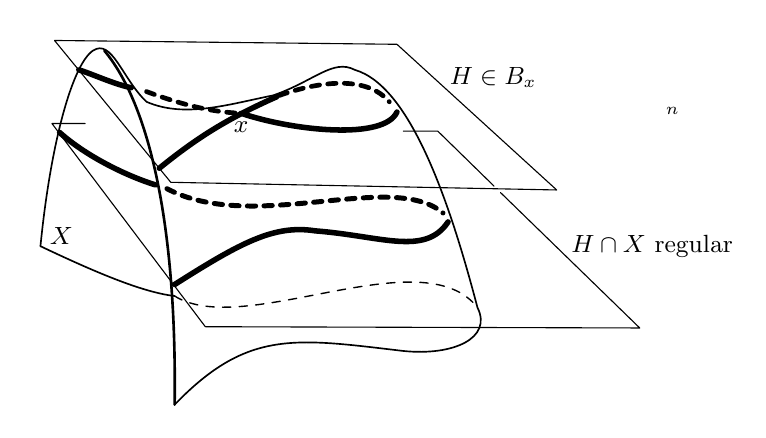
\begin{tikzpicture}[x=.46bp,y=-.46bp,line cap=round,line join=round,font=\small]
\path[use as bounding box] (158,897) rectangle (714,1196);
\draw (179,907)--(447,910)--(572,1024)--(270,1018)--cycle;
\draw (177,972)--(203,972) (452,978)--(479,978)--(523,1021)
      (528,1026)--(637,1132)--(297,1131)--(177,972);
\draw[line width=.6pt] (168,1068) .. controls (176,987) and (193,926) .. (209,915)
  .. controls (224,905) and (232,937) .. (251,955)
  .. controls (281,968) and (315,957) .. (350,950)
  .. controls (382,939) and (397,921) .. (414,930)
  .. controls (459,943) and (490,1040) .. (510,1116)
  .. controls (522,1140) and (491,1154) .. (452,1150)
  .. controls (367,1140) and (330,1133) .. (273,1192);
\draw[line width=.6pt] (168,1068) .. controls (208,1087) and (247,1104) .. (273,1107);
\draw[dashed,line width=.5pt] (273,1107) .. controls (327,1141) and (467,1061) .. (510,1116);
\draw[line width=.95pt] (218,915) .. controls (250,953) and (275,1041) .. (273,1192);
\draw[line width=2pt] (198,930) .. controls (208,933) and (225,941) .. (239,944)
  (261,1007) .. controls (293,981) and (317,967) .. (353,951)
  (325,964) .. controls (367,978) and (437,985) .. (447,963);
\draw[dashed,line width=1.7pt] (251,947) .. controls (278,957) and (301,963) .. (325,964)
  (355,950) .. controls (389,938) and (424,935) .. (441,955);
\draw[line width=2pt] (183,979) .. controls (203,997) and (235,1013) .. (258,1020)
  (273,1098) .. controls (325,1065) and (351,1051) .. (383,1056)
  .. controls (435,1060) and (469,1076) .. (487,1049);
\draw[dashed,line width=1.8pt] (267,1023) .. controls (335,1059) and (443,1008) .. (483,1042);
\node[anchor=west,inner sep=0pt] at (488,936) {$H\in B_x$};
\node[anchor=west,inner sep=0pt] at (657,966) {$\Proj^n$};
\node[anchor=west,inner sep=0pt] at (583,1068) {$H\cap X$ regular};
\node[anchor=west,inner sep=0pt] at (175,1060) {$X$};
\node[anchor=north,inner sep=0pt] at (325,970) {$x$};
\end{tikzpicture}\\[3pt]
\small\hypertarget{fig-book-10}{}Figure 10.\quad Hyperplane sections of a nonsingular variety.
\end{minipage}
}
% Contents from body/page-194.tex.
\ChapterSheet[10.6]{194}{180}{\Goto{p-74}{II\quad Schemes}}{%
\noindent hyperplane $H$ is determined by a nonzero global section $f\in V=\Gamma(\Proj^n,\mathcal O_{\Proj^n}(1))$. Let us fix an $f_0\in V$ such that $x\notin H_0$, the hyperplane defined by $f_0$. Then we can define a map of $k$-vector spaces
\[
\varphi_x\colon V\longrightarrow\mathcal O_{x,X}/\mathfrak m_x^2
\]
\noindent as follows. Given $f\in V$, then $f/f_0$ is a regular function on $\Proj^n-H_0$, which induces a regular function on $X-X\cap H_0$. We take $\varphi_x(f)$ to be the image of $f/f_0$ in the local ring $\mathcal O_{x,X}$ modulo $\mathfrak m_x^2$.
\EditionText{Write $g=(f/f_0)|_X$ near $x$. If $H$ contains $X$, then $g=0$. Otherwise, the local equation $g$ is nonzero, and the scheme $H\cap X$ is defined by $(g)$ at $x$. Then $x\in H\cap X$ if and only if $g\in\mathfrak m_x$, and $x$ lies in a nonregular hyperplane section precisely when $g\in\mathfrak m_x^2$. Thus $\varphi_x(f)=0$ is equivalent to $H\in B_x$.}

Since $x$ is a closed point and $k$ is algebraically closed, $\mathfrak m_x$ is generated by linear forms in the coordinates, so we see that $\varphi_x$ is surjective. If $\dim X=r$, then $\dim_k\mathcal O_x/\mathfrak m_x^2=r+1$. We have $\dim V=n+1$, so $\dim\ker\varphi_x=n-r$. \EditionText{If $r=n$, then $B_x$ is empty for every $x$, and the result follows directly. If $r<n$, then $B_x$ is a linear system of hyperplanes (in the sense of \Goto{sec-II-7}{\S7}) of dimension $n-r-1$.}

Now, considering the complete linear system $|H|$ as a projective space, consider the subset $B\subseteq X\times |H|$ consisting of all pairs $\langle x,H\rangle$ such that $x\in X$ is a closed point and $H\in B_x$. Clearly $B$ is the set of closed points of a closed subset of $X\times |H|$, which we denote also by $B$, and which we give a reduced induced scheme structure. \EditionText{The fibers of the first projection $p_1\colon B\to X$ have dimension $n-r-1$, so $\dim B\le r+(n-r-1)=n-1$.} Therefore, considering the second projection $p_2\colon B\to |H|$, we have $\dim p_2(B)\le n-1$. Since $\dim|H|=n$, we conclude that $p_2(B)<|H|$. If $H\in |H|-p_2(B)$, then $H\nsupseteq X$ and every point of $H\cap X$ is regular, so that $H$ satisfies the requirements of the theorem. Finally note that since $X$ is projective, $p_2\colon X\times |H|\to |H|$ is a proper morphism; $B$ is closed in $X\times |H|$, so $p_2(B)$ is closed in $|H|$. Thus $|H|-p_2(B)$ is an open dense subset of $|H|$, which proves the last statement of the theorem.

\medskip
\noindent\hypertarget{result-II-8.18.1}{}\textbf{Remark 8.18.1.} This result continues to hold even if $X$ has a finite number of singular points, because the set of hyperplanes containing any one of them is a proper closed subset of $|H|$.

\medskip
\emph{Applications}\par
\noindent Now we will apply the preceding ideas to define some invariants of nonsingular varieties over a field.

\Dfn Let $X$ be a nonsingular variety over $k$. We define the \emph{tangent sheaf} of $X$ to be $\mathcal T_X=\mathcal Hom_{\mathcal O_X}(\Omega_{X/k},\mathcal O_X)$. It is a locally free sheaf of rank $n=\dim X$. We define the \emph{canonical sheaf} of $X$ to be $\omega_X=\bigwedge^n\Omega_{X/k}$,
}
% Contents from body/page-195.tex.
\ChapterSheet{195}{181}{\Goto{sec-II-8}{8\quad Differentials}}{%
\noindent the $n$th exterior power of the sheaf of differentials, where $n=\dim X$. It is an invertible sheaf on $X$. If $X$ is projective and nonsingular, we define the \emph{geometric genus} of $X$ to be $p_g=\dim_k\Gamma(X,\omega_X)$. It is a nonnegative integer.

\medskip
\noindent\hypertarget{result-II-8.18.2}{}\textbf{Remark 8.18.2.} Earlier (I, Ex.~\Goto{ex-I-7.2}{7.2}) we defined the arithmetic genus $p_a$ of a variety in projective space. In the case of a projective nonsingular curve, the arithmetic genus and the geometric genus coincide. This is a consequence of the Serre duality theorem which we will prove later (III, \Goto{result-III-7.12.2}{7.12.2}). For varieties of dimension $\ge2$, however, $p_a$ and $p_g$ need not be equal (Ex.~\Goto{ex-II-8.3}{8.3}). See also (III, \Goto{result-III-7.12.3}{7.12.3}).

\medskip
\noindent\hypertarget{result-II-8.18.3}{}\textbf{Remark 8.18.3.} Since the sheaf of differentials, the tangent sheaf, and the canonical sheaf are all defined intrinsically, any numbers which we can define from them, such as the geometric genus, are invariants of $X$ up to isomorphism. In fact, we will now show that the geometric genus is a \emph{birational invariant} of a nonsingular projective variety. This makes it extremely important for the classification problem.

\medskip
\noindent\hypertarget{result-II-8.19}{}\textbf{Theorem 8.19.} \emph{Let $X$ and $X'$ be two birationally equivalent nonsingular projective varieties over $k$. Then $p_g(X)=p_g(X')$.}

\Proof Recall from (I, \S\Goto{sec-I-4}{4}) that for $X$ and $X'$ to be birationally equivalent means that there are rational maps from $X$ to $X'$ and from $X'$ to $X$ which are inverses to each other. Considering the rational map from $X$ to $X'$, let $V\subseteq X$ be the largest open set for which there is a morphism $f\colon V\to X'$ representing this rational map. Then from (\Goto{result-II-8.11}{8.11}) we have a map $f^*\Omega_{X'/k}\to\Omega_{V/k}$. These are locally free sheaves of the same rank $n=\dim X$, so we get an induced map on the exterior powers: $f^*\omega_{X'}\to\omega_V$. This map in turn induces a map on the space of global sections $f^*\colon\Gamma(X',\omega_{X'})\to\Gamma(V,\omega_V)$. Now since $f$ is birational, by (I, \Goto{result-I-4.5}{4.5}), there is an open set $U\subseteq V$ such that $f(U)$ is open in $X'$, and $f$ induces an isomorphism from $U$ to $f(U)$. Thus $\omega_V|_U\cong\omega_{X'}|_{f(U)}$ via $f$. Since a nonzero global section of an invertible sheaf cannot vanish on a dense open set, we conclude that the map of vector spaces $f^*\colon\Gamma(X',\omega_{X'})\to\Gamma(V,\omega_V)$ must be injective.

Next we will compare $\Gamma(V,\omega_V)$ with $\Gamma(X,\omega_X)$. First I claim that $X-V$ has codimension $\ge2$ in $X$. Indeed, this follows from the valuative criterion of properness (\Goto{result-II-4.7}{4.7}). If $P\in X$ is a point of codimension $1$, then $\mathcal O_{P,X}$ is a discrete valuation ring (because $X$ is nonsingular). We already have a map of the generic point of $X$ to $X'$; and $X'$ is projective, hence proper over $k$, so there exists a unique morphism $\operatorname{Spec}\mathcal O_{P,X}\to X'$ compatible with the given birational map. This extends to a morphism of some neighborhood of $P$ to $X'$, so we must have $P\in V$ by definition of $V$.

Now we can show that the natural restriction map $\Gamma(X,\omega_X)\to\Gamma(V,\omega_V)$ is bijective. It is enough to show, for any open affine subset $U\subseteq X$ such that
}
% Contents from body/page-196.tex.
\ChapterSheet{196}{182}{\Goto{p-74}{II\quad Schemes}}{%
\noindent $\omega_X|_U\cong\mathcal O_U$, that $\Gamma(U,\mathcal O_U)\to\Gamma(U\cap V,\mathcal O_{U\cap V})$ is bijective. Since $X$ is nonsingular, hence normal, and since $U-U\cap V$ has codimension $\ge2$ in $U$, this is an immediate consequence of (\Goto{result-II-6.3A}{6.3A}).

Combining our results, we see that $p_g(X')\le p_g(X)$. We obtain the reverse inequality by symmetry, and thus conclude that $p_g(X)=p_g(X')$.

\smallskip
Next we study the behavior of the tangent sheaf and the canonical sheaf for a nonsingular subvariety of a variety $X$.

\Dfn Let $Y$ be a nonsingular subvariety of a nonsingular variety $X$ over $k$. The locally free sheaf $\mathcal I/\mathcal I^2$ of (\Goto{result-II-8.17}{8.17}) we call the \emph{conormal} sheaf of $Y$ in $X$. Its dual $\mathcal N_{Y/X}=\mathcal Hom_{\mathcal O_Y}(\mathcal I/\mathcal I^2,\mathcal O_Y)$ is called the \emph{normal sheaf} of $Y$ in $X$. It is locally free of rank $r=\operatorname{codim}(Y,X)$.

\smallskip
Note that if we take the dual on $Y$ of the exact sequence of locally free sheaves on $Y$ given in (\Goto{result-II-8.17}{8.17}), then we obtain an exact sequence
\[
0\longrightarrow\mathcal T_Y\longrightarrow\mathcal T_X\otimes\mathcal O_Y
  \longrightarrow\mathcal N_{Y/X}\longrightarrow0.
\]
\noindent This shows that the normal sheaf we have just defined corresponds to the usual geometric notion of normal vectors being tangent vectors of the ambient space modulo tangent vectors of the subspace.

\medskip
\noindent\hypertarget{result-II-8.20}{}\textbf{Proposition 8.20.} \emph{Let $Y$ be a nonsingular subvariety of codimension $r$ in a nonsingular variety $X$ over $k$. Then $\omega_Y\cong\omega_X\otimes\bigwedge^r\mathcal N_{Y/X}$. In case $r=1$, consider $Y$ as a divisor, and let $\mathcal L$ be the associated invertible sheaf on $X$. Then $\omega_Y\cong\omega_X\otimes\mathcal L\otimes\mathcal O_Y$.}

\Proof We take the highest exterior powers of the locally free sheaves in the exact sequence
\[
0\longrightarrow\mathcal I/\mathcal I^2\longrightarrow\Omega_X\otimes\mathcal O_Y
  \longrightarrow\Omega_Y\longrightarrow0
\]
\noindent (Ex.~\Goto{ex-II-5.16}{5.16d}). Thus we find that $\omega_X\otimes\mathcal O_Y\cong\omega_Y\otimes\bigwedge^r(\mathcal I/\mathcal I^2)$. Since formation of the highest exterior power commutes with taking the dual sheaf, we find $\omega_Y\cong\omega_X\otimes\bigwedge^r\mathcal N_{Y/X}$. In the special case $r=1$, we have $\mathcal I_Y\cong\mathcal L^{-1}$ by (\Goto{result-II-6.18}{6.18}). Thus $\mathcal I/\mathcal I^2\cong\mathcal L^{-1}\otimes\mathcal O_Y$, and $\mathcal N_{Y/X}\cong\mathcal L\otimes\mathcal O_Y$. So applying the previous result with $r=1$, we obtain $\omega_Y\cong\omega_X\otimes\mathcal L\otimes\mathcal O_Y$.

\medskip
\noindent\hypertarget{result-II-8.20.1}{}\textbf{Example 8.20.1.} Let $X=\Proj_k^n$. Taking the dual of the exact sequence of (\Goto{result-II-8.13}{8.13}) gives us this exact sequence involving the tangent sheaf of $\Proj^n$:
\[
0\longrightarrow\mathcal O_X\longrightarrow\mathcal O_X(1)^{n+1}
  \longrightarrow\mathcal T_X\longrightarrow0.
\]
\noindent To obtain the canonical sheaf of $\Proj^n$, we take the highest exterior powers of the exact sequence of (\Goto{result-II-8.13}{8.13}) and we find $\omega_X\cong\mathcal O_X(-n-1)$. Since $\mathcal O(l)$ has no global sections for $l<0$, we find that $p_g(\Proj^n)=0$ for any $n\ge1$. Recall that a \emph{rational variety} is defined as a variety birational to $\Proj^n$ for some $n$
}
% Contents from body/page-197.tex.
\ChapterSheet[10.7]{197}{183}{\Goto{sec-II-8}{8\quad Differentials}}{%
\noindent (I, Ex.~\Goto{ex-I-4.4}{4.4}). We conclude from (\Goto{result-II-8.19}{8.19}) that if $X$ is \EditionText{a nonsingular projective rational variety of positive dimension}, then $p_g(X)=0$. This fact will enable us to demonstrate the existence of nonrational varieties \EditionText{in every positive dimension}.

\medskip
\noindent\hypertarget{result-II-8.20.2}{}\textbf{Example 8.20.2.} Let $X=\Proj_k^n$, with $n\ge2$. For any integer $d\ge1$, the divisor $dH$, where $H$ is a hyperplane, is a very ample divisor (\Goto{result-II-7.6.1}{7.6.1}). Thus $dH$ becomes a hyperplane section of $X$ in a suitable projective embedding (the $d$-uple embedding), and we can apply Bertini's theorem (\Goto{result-II-8.18}{8.18}). We find that there is a subscheme $Y\in |dH|$ which is regular at every one of its points. If $Y$ had at least two irreducible components, say $Y_1$ and $Y_2$, then since $n\ge2$, their intersection $Y_1\cap Y_2$ would be nonempty (I, \Goto{result-I-7.2}{7.2}). But this cannot happen because $Y$ would be singular at any point of $Y_1\cap Y_2$, so we conclude in fact that $Y$ is irreducible, hence a nonsingular variety. Thus we see for any $d\ge1$ that there are nonsingular hypersurfaces of degree $d$ in $\Proj^n$. In fact, they form a dense open subset of the complete linear system $|dH|$. (This generalizes (I, Ex.~\Goto{ex-I-5.5}{5.5}).)

\medskip
\noindent\hypertarget{result-II-8.20.3}{}\textbf{Example 8.20.3.} Let $Y$ be a nonsingular hypersurface of degree $d$ in $\Proj^n$, $n\ge2$. Then from (\Goto{result-II-8.20}{8.20}) and the first example above, we conclude that $\omega_Y\cong\mathcal O_Y(d-n-1)$. Let's look at some particular cases.

$n=2$, $d=1$. $Y$ is a line in $\Proj^2$, so $Y\cong\Proj^1$, and we have $\omega_Y\cong\mathcal O_Y(-2)$ which we already knew.

$n=2$, $d=2$. $Y$ is a conic in $\Proj^2$, and $\omega_Y\cong\mathcal O_Y(-1)$. In this case $Y$ is the 2-uple embedding of $\Proj^1$, so pulling $\omega_Y$ back to $\Proj^1$ gives $\omega_{\Proj^1}\cong\mathcal O_{\Proj^1}(-2)$, which is again what we already knew.

$n=2$, $d=3$. $Y$ is a nonsingular plane cubic curve, and $\omega_Y\cong\mathcal O_Y$. Therefore $p_g(Y)=\dim\Gamma(Y,\mathcal O_Y)=1$, and we see that $Y$ is not rational! This generalizes (I, Ex.~\Goto{ex-I-6.2}{6.2}), where we gave just one example of a nonsingular cubic curve, and showed by a different method that it was not rational.

$n=2$, $d\ge4$. $Y$ is a nonsingular plane curve of degree $d$, $\omega_Y\cong\mathcal O_Y(d-3)$, and $d-3>0$. Hence $p_g>0$, and $Y$ is not rational. In fact, $p_g=\frac12(d-1)(d-2)$ (Ex.~\Goto{ex-II-8.4f}{8.4f}), so we see that plane curves of different degrees $d,d'\ge3$ are not birational to each other. Another way of seeing this is as follows. For any nonsingular projective curve, we can consider the \emph{degree} of the canonical sheaf. Since a nonsingular projective curve is unique in its birational equivalence class (I, \S\Goto{sec-I-6}{6}), this number is in fact a birational invariant. In the present case its value is $d(d-3)$, since $\mathcal O(1)$ has degree $d$ on $Y$. These numbers are also distinct for different $d,d'\ge3$. This shows the existence of infinitely many mutually nonbirational curves.

$n=3$, $d=1$. This gives $Y\cong\Proj^2$, $\omega_Y\cong\mathcal O_Y(-3)$ which we knew.

$n=3$, $d=2$. Here $Y$ is a nonsingular quadric surface, and $\omega_Y\cong\mathcal O_Y(-2)$. We have $p_g(Y)=0$, which is consistent with the fact that $Y$ is rational (I, Ex.~\Goto{ex-I-4.5}{4.5}). In terms of the isomorphism $Y\cong\Proj^1\times\Proj^1$, $\omega_Y$ corresponds to a divisor class of type $(-2,-2)$---see (\Goto{result-II-6.6.1}{6.6.1}). This illustrates the general fact
}
% Contents from body/page-198.tex.
\ChapterSheet[10.8]{198}{184}{\Goto{p-74}{II\quad Schemes}}{%
\noindent (Ex.~\Goto{ex-II-8.3}{8.3}) that the canonical sheaf on a direct product of nonsingular varieties is the tensor product of the pull-backs of the canonical sheaves on the two factors.

$n=3$, $d=3$. $Y$ is a nonsingular cubic surface in $\Proj^3$, $\omega_Y\cong\mathcal O_Y(-1)$ and so $p_g(Y)=0$. In this case also, $Y$ is a rational surface, as we will see later (Chapter~\Goto{p-370}{V}).

$n=3$, $d=4$. In this case $\omega_Y\cong\mathcal O_Y$. The canonical sheaf is trivial so $p_g=1$. This is a nonrational surface which belongs to the class of \textquotedblleft{}K3 surfaces.\textquotedblright{}

$n=3$, $d\ge5$. Here $\omega_Y\cong\mathcal O_Y(d-4)$ with $d-4>0$. Hence $p_g>0$, and $Y$ is not rational. Surfaces such as these on which the canonical sheaf is very ample belong to the class of \textquotedblleft{}surfaces of general type.\textquotedblright{}

$n=4$, $d=3,4$. The cubic and the quartic threefold in $\Proj^4$ both have $p_g=0$, but it has recently been shown (by different methods) that they are not in general rational varieties. For the cubic threefold, see Clemens and Griffiths \Goto{bib-clemens-griffiths-1}{[1]}. For the quartic threefold, see Iskovskih and Manin \Goto{bib-iskovskih-manin-1}{[1]}.

\EditionText{$n\ge2$, $d\ge n+1$.} In this case we obtain a nonsingular hypersurface $Y$ in $\Proj^n$, with $\omega_Y\cong\mathcal O_Y(d-n-1)$ and $d-n-1\ge0$. Hence $p_g(Y)\ge1$, and so $Y$ is not rational. This shows the existence of nonrational varieties \EditionText{in every positive dimension}.

\medskip
\emph{Some Local Algebra}\par
\noindent Here we will gather some results from local algebra, mainly concerning depth and Cohen--Macaulay rings, which are useful in algebraic geometry. Then we relate them to the geometric notion of local complete intersection, and give an application to blowing up. We refer to Matsumura [\Goto{bib-479-17}{2}, Ch.~6] for proofs.

If $A$ is a ring, and $M$ is an $A$-module, recall that a sequence $x_1,\ldots,x_r$ of elements of $A$ is called a \emph{regular sequence} for $M$ if $x_1$ is not a zero divisor in $M$, and for all $i=2,\ldots,r$, $x_i$ is not a zero divisor in $M/(x_1,\ldots,x_{i-1})M$. \EditionText{If $A$ is a noetherian local ring with the maximal ideal $\mathfrak m$ and $M$ is a nonzero finitely generated $A$-module,} then the \emph{depth} of $M$ is the maximum length of a regular sequence $x_1,\ldots,x_r$ for $M$ with all $x_i\in\mathfrak m$. These definitions apply to the ring $A$ itself, and we say that a local noetherian ring $A$ is \emph{Cohen--Macaulay} if $\operatorname{depth}A=\dim A$. Now we list some properties of Cohen--Macaulay rings.

\medskip
\noindent\hypertarget{result-II-8.21A}{}\textbf{Theorem 8.21A.} \emph{Let $A$ be a local noetherian ring with maximal ideal $\mathfrak m$.}
\begin{parts}
\item\hypertarget{result-II-8.21Aa}{} \emph{If $A$ is regular, then it is Cohen--Macaulay.}
\item\hypertarget{result-II-8.21Ab}{} \emph{If $A$ is Cohen--Macaulay, then any localization of $A$ at a prime ideal is also Cohen--Macaulay.}
\item\hypertarget{result-II-8.21Ac}{} \emph{If $A$ is Cohen--Macaulay, then a set of elements $x_1,\ldots,x_r\in\mathfrak m$ forms a regular sequence for $A$ if and only if $\dim A/(x_1,\ldots,x_r)=\dim A-r$.}
\item\hypertarget{result-II-8.21Ad}{} \emph{If $A$ is Cohen--Macaulay, and $x_1,\ldots,x_r\in\mathfrak m$ is a regular sequence for $A$, then $A/(x_1,\ldots,x_r)$ is also Cohen--Macaulay.}
\end{parts}
}
% Contents from body/page-199.tex.
\ChapterSheet{199}{185}{\Goto{sec-II-8}{8\quad Differentials}}{%
\begin{parts}
\item[(e)]\hypertarget{result-II-8.21Ae}{} \emph{If $A$ is Cohen--Macaulay, and $x_1,\ldots,x_r\in\mathfrak m$ is a regular sequence, let $I$ be the ideal $(x_1,\ldots,x_r)$. Then the natural map $(A/I)[t_1,\ldots,t_r]\to\operatorname{gr}_I A=\bigoplus_{n\ge0}I^n/I^{n+1}$, defined by sending $t_i\mapsto x_i$, is an isomorphism. In other words, $I/I^2$ is a free $A/I$-module of rank $r$, and for each $n\ge1$, the natural map $S^n(I/I^2)\to I^n/I^{n+1}$ is an isomorphism, where $S^n$ denotes the $n$th symmetric power.}
\end{parts}
\noindent\textsc{Proofs.}\enspace Matsumura [\Goto{bib-479-17}{2}: (\Goto{result-II-8.21Aa}{a}) p.~121; (\Goto{result-II-8.21Ab}{b}) p.~104; (\Goto{result-II-8.21Ac}{c}) p.~105; (\Goto{result-II-8.21Ad}{d}) p.~104; (\Goto{result-II-8.21Ae}{e}) p.~110].

\smallskip
In keeping with the terminology for schemes (Ex.~\Goto{ex-II-3.8}{3.8}), we will say that a noetherian ring $A$ is \emph{normal} if for every prime ideal $\mathfrak p$, the localization $A_{\mathfrak p}$ is an integrally closed domain. A normal ring is a finite direct product of integrally closed domains.

\medskip
\noindent\hypertarget{result-II-8.22A}{}\textbf{Theorem 8.22A} (Serre). \emph{A noetherian ring $A$ is normal if and only if it satisfies the following two conditions:}
\begin{enumerate}[label=(\arabic*),leftmargin=2.4em,topsep=4pt,itemsep=0pt]
\item\hypertarget{cond-II-8.22A-1}{} \emph{for every prime ideal $\mathfrak p\subseteq A$ of height $\le1$, $A_{\mathfrak p}$ is regular (hence a field or a discrete valuation ring); and}
\item\hypertarget{cond-II-8.22A-2}{} \emph{for every prime ideal $\mathfrak p\subseteq A$ of height $\ge2$, we have $\operatorname{depth}A_{\mathfrak p}\ge2$.}
\end{enumerate}
\Proof Matsumura [\Goto{bib-479-17}{2}, Th.~39, p.~125]. Condition (\Goto{cond-II-8.22A-1}{1}) is sometimes called \textquotedblleft{}$R_1$\textquotedblright{}, or \textquotedblleft{}regular in codimension 1\textquotedblright{}. Condition (\Goto{cond-II-8.22A-2}{2}), supplemented by the requirement that for $\operatorname{ht}\mathfrak p=1$, $\operatorname{depth}A_{\mathfrak p}=1$, which is a consequence of (\Goto{cond-II-8.22A-1}{1}) in our case, is called the \textquotedblleft{}condition $S_2$ of Serre\textquotedblright{}.

\smallskip
Now we apply these results to algebraic geometry. We will say that a scheme is \emph{Cohen--Macaulay} if all of its local rings are Cohen--Macaulay.

\Dfn Let $Y$ be a closed subscheme of a nonsingular variety $X$ over $k$. We say that $Y$ is a \emph{local complete intersection} in $X$ if the ideal sheaf $\mathcal I_Y$ of $Y$ in $X$ can be locally generated by $r=\operatorname{codim}(Y,X)$ elements at every point.

\medskip
\noindent\hypertarget{result-II-8.22.1}{}\textbf{Example 8.22.1.} If $Y$ itself is nonsingular, then by (\Goto{result-II-8.17}{8.17}) it is a local complete intersection inside any nonsingular $X$ which contains it.

\medskip
\noindent\hypertarget{result-II-8.22.2}{}\textbf{Remark 8.22.2.} In fact, the notion of being a local complete intersection is an intrinsic property of the scheme $Y$, i.e., independent of the nonsingular variety containing it. This is proved using the cotangent complex of a morphism, which extends the concept of relative differentials introduced above---see Lichtenbaum and Schlessinger \Goto{bib-479-6-item-1}{[1]}. We will not use this fact in the sequel.
}
% Contents from body/page-200.tex.
\ChapterSheet{200}{186}{\Goto{p-74}{II\quad Schemes}}{%
\noindent\hypertarget{result-II-8.23}{}\textbf{Proposition 8.23.} \emph{Let $Y$ be a locally complete intersection subscheme of a nonsingular variety $X$ over $k$. Then:}

\noindent\hspace*{1.7em}(a) \emph{$Y$ is Cohen--Macaulay;}

\noindent\hspace*{1.7em}(b) \emph{$Y$ is normal if and only if it is regular in codimension $1$.}

\smallskip
\noindent\textsc{Proof.}

(a) Since $X$ is nonsingular, it is Cohen--Macaulay by (\Goto{result-II-8.21A}{8.21Aa}). Since $\mathcal I_Y$ is locally generated by $r=\operatorname{codim}(Y,X)$ elements, those elements locally form a regular sequence in $\mathcal O_X$, by (\Goto{result-II-8.21A}{8.21Ac}), and so $Y$ is Cohen--Macaulay by (\Goto{result-II-8.21A}{8.21Ad}).

(b) We already know that normal implies regular in codimension $1$ (I, \Goto{result-I-6.2A}{6.2A}). For the converse, we use (\Goto{result-II-8.22A}{8.22A}) applied to the local rings of $Y$. Condition (\Goto{result-II-8.22A}{1}) is our hypothesis, and condition (\Goto{result-II-8.22A}{2}) holds automatically because $Y$ is Cohen--Macaulay.

\medskip
As our last application, we consider the blowing-up of a nonsingular variety along a nonsingular subvariety (cf.\ \Goto{sec-II-7}{\S7} for definition of blowing-up). The following theorem will be useful in comparing invariants of $X$ and $\widetilde X$ (Ex.~\Goto{ex-II-8.5}{8.5}).

\medskip
\noindent\hypertarget{result-II-8.24}{}\textbf{Theorem 8.24.} \emph{Let $X$ be a nonsingular variety over $k$, and let \EditionText{$Y\subsetneq X$} be a nonsingular closed subvariety, with ideal sheaf $\mathcal I$. Let $\pi\colon\widetilde X\to X$ be the blowing-up of $\mathcal I$, and let $Y'\subseteq\widetilde X$ be the subscheme defined by the inverse image ideal sheaf $\mathcal I'=\pi^{-1}\mathcal I\cdot\mathcal O_{\widetilde X}$. Then:}

\noindent\hangindent=3em\hspace*{1.7em}\hypertarget{result-II-8.24-a}{}(a) \emph{$\widetilde X$ is also nonsingular;}

\noindent\hangindent=3em\hspace*{1.7em}\hypertarget{result-II-8.24-b}{}(b) \emph{$Y'$, together with the induced projection map $\pi\colon Y'\to Y$, is isomorphic to $\mathbf P(\mathcal I/\mathcal I^2)$, the projective space bundle associated to the (locally free) sheaf $\mathcal I/\mathcal I^2$ on $Y$;}

\noindent\hangindent=3em\hspace*{1.7em}\hypertarget{result-II-8.24-c}{}(c) \emph{under this isomorphism, the normal sheaf $\mathcal N_{Y'/\widetilde X}$ corresponds to $\mathcal O_{\mathbf P(\mathcal I/\mathcal I^2)}(-1)$.}

\smallskip
\noindent\textsc{Proof.} We prove \Goto{result-II-8.24-b}{(b)} first. Since $\widetilde X=\operatorname{Proj}\bigoplus\mathcal I^d$, we have
\[
Y'\cong\operatorname{Proj}\bigoplus(\mathcal I^d\otimes\mathcal O_X/\mathcal I)=\operatorname{Proj}\bigoplus\mathcal I^d/\mathcal I^{d+1}.
\]
But $Y$ is nonsingular, so $\mathcal I$ is locally generated by a regular sequence in $\mathcal O_X$, and we can apply (\Goto{result-II-8.21A}{8.21Ae}). This implies that $\mathcal I/\mathcal I^2$ is locally free and that for each $n\ge1$, $\mathcal I^n/\mathcal I^{n+1}\cong S^n(\mathcal I/\mathcal I^2)$. Thus $Y'\cong\operatorname{Proj}\bigoplus S^d(\mathcal I/\mathcal I^2)$, which by definition is $\mathbf P(\mathcal I/\mathcal I^2)$.

In particular, $Y'$ is locally isomorphic to $Y\times\mathbf P^{r-1}$, where $r=\operatorname{codim}(Y,X)$, so $Y'$ is also nonsingular. Since $Y'$ is locally principal in $\widetilde X$ (\Goto{result-II-7.13}{7.13a}), it follows that $\widetilde X$ is also nonsingular\EditionText{. Away from $Y'$ the blow-up is isomorphic to $X-Y$, while at points of $Y'$ a quotient of a noetherian local ring by a non-zero-divisor is regular only if the local ring itself is regular.}

To prove \Goto{result-II-8.24-c}{(c)}, we recall from the proof of (\Goto{result-II-7.13}{7.13}) that $\mathcal I'=\pi^{-1}(\mathcal I)\cdot\mathcal O_{\widetilde X}$ is isomorphic to $\mathcal O_{\widetilde X}(1)$. It follows that $\mathcal I'/\mathcal I'^2\cong\mathcal O_{Y'}(1)$, and hence $\mathcal N_{Y'/\widetilde X}\cong\mathcal O_{Y'}(-1)$.}
% Contents from body/page-201.tex.
\ChapterSheet[10.7]{201}{187}{\Goto{sec-II-8}{8\quad Differentials}}{%
We will use the following algebraic result in the exercises.

\medskip
\noindent\hypertarget{result-II-8.25A}{}\textbf{Theorem 8.25A} (I.~S.~Cohen). \emph{Let $A$ be a complete local ring containing a field $k$. Assume that the residue field $k(A)=A/\mathfrak m$ is a separably generated extension of $k$. Then there is a subfield $K\subseteq A$, containing $k$, such that $K\to A/\mathfrak m$ is an isomorphism. (The subfield $K$ is called a \textup{field of representatives} for $A$.)}

\smallskip
\noindent\textsc{Proof.} Matsumura \Goto{bib-479-17}{[2, p.~205]}.

\medskip
\noindent\textsc{Exercises}

\smallskip
\noindent\hypertarget{ex-II-8.1}{}\textbf{8.1.} Here we will strengthen the results of the text to include information about the sheaf of differentials at a not necessarily closed point of a scheme $X$.

\noindent\hangindent=3em\hspace*{1.7em}(a) Generalize (\Goto{result-II-8.7}{8.7}) as follows. Let $B$ be a local ring containing a field $k$, and assume that the residue field $k(B)=B/\mathfrak m$ of $B$ is a separably generated extension of $k$. Then the exact sequence of (\Goto{result-II-8.4A}{8.4A}),
\[
0\longrightarrow\mathfrak m/\mathfrak m^2\xrightarrow{d}\Omega_{B/k}\otimes k(B)\longrightarrow\Omega_{k(B)/k}\longrightarrow0
\]
is exact on the left also. [\emph{Hint:} In copying the proof of (\Goto{result-II-8.7}{8.7}), first pass to $B/\mathfrak m^2$, which is a complete local ring, and then use (\Goto{result-II-8.25A}{8.25A}) to choose a field of representatives for $B/\mathfrak m^2$.]

\noindent\hangindent=3em\hspace*{1.7em}(b) Generalize (\Goto{result-II-8.8}{8.8}) as follows. With $B,k$ as above, assume furthermore that $k$ is perfect, and that $B$ is a localization of an algebra of finite type over $k$. Then show that $B$ is a regular local ring if and only if $\Omega_{B/k}$ is free of rank $=\dim B+\operatorname{tr.d.}k(B)/k$.

\noindent\hangindent=3em\hspace*{1.7em}(c) Strengthen (\Goto{result-II-8.15}{8.15}) as follows. Let $X$ be an irreducible scheme of finite type over a perfect field $k$, and let $\dim X=n$. For any point $x\in X$, not necessarily closed, show that the local ring $\mathcal O_{x,X}$ is a regular local ring if and only if the stalk $(\Omega_{X/k})_x$ of the sheaf of differentials at $x$ is free of rank $n$.

\noindent\hangindent=3em\hspace*{1.7em}(d) Strengthen (\Goto{result-II-8.16}{8.16}) as follows. If $X$ is a variety over an algebraically closed field $k$, then $U=\{x\in X\mid\mathcal O_x\text{ is a regular local ring}\}$ is an open dense subset of $X$.

\smallskip
\noindent\hypertarget{ex-II-8.2}{}\textbf{8.2.} Let $X$ be a variety of dimension $n$ over $k$. Let $\mathcal E$ be a locally free sheaf of rank $>n$ on $X$, and let $V\subseteq\Gamma(X,\mathcal E)$ be a vector space of global sections which generate $\mathcal E$. Then show that there is an element $s\in V$, such that for each $x\in X$, we have $s_x\notin\mathfrak m_x\mathcal E_x$. Conclude that there is a morphism $\mathcal O_X\to\mathcal E$ giving rise to an exact sequence
\[
0\longrightarrow\mathcal O_X\longrightarrow\mathcal E\longrightarrow\mathcal E'\longrightarrow0
\]
where $\mathcal E'$ is also locally free. [\emph{Hint:} Use a method similar to the proof of Bertini's theorem (\Goto{result-II-8.18}{8.18}).]

\smallskip
\noindent\hypertarget{ex-II-8.3}{}\textbf{8.3.} \emph{Product Schemes.}

\noindent\hangindent=3em\hspace*{1.7em}(a) Let $X$ and $Y$ be schemes over another scheme $S$. Use (\Goto{result-II-8.10}{8.10}) and (\Goto{result-II-8.11}{8.11}) to show that $\Omega_{X\times_S Y/S}\cong p_1^*\Omega_{X/S}\oplus p_2^*\Omega_{Y/S}$.

\noindent\hangindent=3em\hspace*{1.7em}(b) If $X$ and $Y$ are nonsingular varieties over a field $k$, show that $\omega_{X\times Y}\cong p_1^*\omega_X\otimes p_2^*\omega_Y$.}
% Contents from body/page-202.tex.
\ChapterSheet[10.5]{202}{188}{\Goto{p-74}{II\quad Schemes}}{%
\fontsize{9.5}{10.5}\selectfont%
\setlength{\parskip}{0pt}%
\setlength{\smallskipamount}{2pt}%
\noindent\hangindent=3em\hspace*{1.7em}(c) Let $Y$ be a nonsingular plane cubic curve, and let $X$ be the surface $Y\times Y$. Show that $p_g(X)=1$ but $p_a(X)=-1$ (I, Ex.~\Goto{ex-I-7.2}{7.2}). This shows that the arithmetic genus and the geometric genus of a nonsingular projective variety may be different.

\smallskip
\noindent\hypertarget{ex-II-8.4}{}\textbf{8.4.} \emph{Complete Intersections in $\mathbf P^n$.} A closed subscheme $Y$ of $\mathbf P_k^n$ is called a \emph{(strict, global) complete intersection} if the homogeneous ideal $I$ of $Y$ in $S=k[x_0,\ldots,x_n]$ can be generated by $r=\operatorname{codim}(Y,\mathbf P^n)$ elements (I, Ex.~\Goto{ex-I-2.17}{2.17}).

\noindent\hangindent=3em\hspace*{1.7em}(a) Let $Y$ be a closed subscheme of codimension $r$ in $\mathbf P^n$. Then $Y$ is a complete intersection if and only if there are hypersurfaces (i.e., locally principal subschemes of codimension $1$) $H_1,\ldots,H_r$, such that $Y=H_1\cap\cdots\cap H_r$ \emph{as schemes}, i.e., $\mathcal I_Y=\mathcal I_{H_1}+\cdots+\mathcal I_{H_r}$. [\emph{Hint:} Use the fact that the unmixedness theorem holds in $S$ (Matsumura \Goto{bib-479-17}{[2, p.~107]}).]

\noindent\hangindent=3em\hspace*{1.7em}\hypertarget{ex-II-8.4-b}{}(b) If $Y$ is a complete intersection of dimension $\ge1$ in $\mathbf P^n$, and if $Y$ is normal, then $Y$ is projectively normal (Ex.~\Goto{ex-II-5.14}{5.14}). [\emph{Hint:} Apply (\Goto{result-II-8.23}{8.23}) to the affine cone over $Y$.]

\noindent\hangindent=3em\hspace*{1.7em}\hypertarget{ex-II-8.4-c}{}(c) With the same hypotheses as \Goto{ex-II-8.4-b}{(b)}, conclude that for all $l\ge0$, the natural map $\Gamma(\mathbf P^n,\mathcal O_{\mathbf P^n}(l))\to\Gamma(Y,\mathcal O_Y(l))$ is surjective. In particular, taking $l=0$, show that $Y$ is connected.

\noindent\hangindent=3em\hspace*{1.7em}\hypertarget{ex-II-8.4-d}{}(d) Now suppose given integers $d_1,\ldots,d_r\ge1$, with $r<n$. Use Bertini's theorem (\Goto{result-II-8.18}{8.18}) to show that there exist nonsingular hypersurfaces $H_1,\ldots,H_r$ in $\mathbf P^n$, with $\deg H_i=d_i$, such that the scheme $Y=H_1\cap\cdots\cap H_r$ is irreducible and nonsingular of codimension $r$ in $\mathbf P^n$.

\noindent\hangindent=3em\hspace*{1.7em}\hypertarget{ex-II-8.4-e}{}(e) If $Y$ is a nonsingular complete intersection as in \Goto{ex-II-8.4-d}{(d)}, show that $\omega_Y\cong\mathcal O_Y(\sum d_i-n-1)$.

\noindent\hangindent=3em\hspace*{1.7em}\hypertarget{ex-II-8.4f}{}(f) If $Y$ is a nonsingular hypersurface of degree $d$ in $\mathbf P^n$\EditionText{ with $n\ge2$}, use \Goto{ex-II-8.4-c}{(c)} and \Goto{ex-II-8.4-e}{(e)} above to show that $p_g(Y)=\binom{d-1}{n}$. Thus $p_g(Y)=p_a(Y)$ (I, Ex.~\Goto{ex-I-7.2}{7.2}). In particular, if $Y$ is a nonsingular plane curve of degree $d$, then $p_g(Y)=\frac12(d-1)(d-2)$.

\noindent\hangindent=3em\hspace*{1.7em}(g) If $Y$ is a nonsingular curve in $\mathbf P^3$, which is a complete intersection of nonsingular surfaces of degrees $d,e$, then $p_g(Y)=\frac12de(d+e-4)+1$. Again the geometric genus is the same as the arithmetic genus (I, Ex.~\Goto{ex-I-7.2}{7.2}).

\smallskip
\noindent\hypertarget{ex-II-8.5}{}\textbf{8.5.} \emph{Blowing up a Nonsingular Subvariety.} As in (\Goto{result-II-8.24}{8.24}), let $X$ be a nonsingular variety, let $Y$ be a nonsingular subvariety of codimension $r\ge2$, let $\pi\colon\widetilde X\to X$ be the blowing-up of $X$ along $Y$, and let $Y'=\pi^{-1}(Y)$.

\noindent\hangindent=3em\hspace*{1.7em}\hypertarget{ex-II-8.5-a}{}(a) Show that the maps $\pi^*\colon\operatorname{Pic} X\to\operatorname{Pic}\widetilde X$, and $\mathbb Z\to\operatorname{Pic}\widetilde X$ defined by $n\mapsto\text{class of }nY'$, give rise to an isomorphism $\operatorname{Pic}\widetilde X\cong\operatorname{Pic} X\oplus\mathbb Z$.

\noindent\hangindent=3em\hspace*{1.7em}(b) Show that $\omega_{\widetilde X}\cong\EditionText{\pi^*}\omega_X\otimes\mathcal L((r-1)Y')$. [\emph{Hint:} By \Goto{ex-II-8.5-a}{(a)} we can write in any case $\omega_{\widetilde X}\cong\EditionText{\pi^*}\mathcal M\otimes\mathcal L(qY')$ for some invertible sheaf $\mathcal M$ on $X$, and some integer $q$. By restricting to $\widetilde X-Y'\cong X-Y$, show that $\mathcal M\cong\omega_X$. To determine $q$, proceed as follows. First show that $\omega_{Y'}\cong\EditionText{(\pi|_{Y'})^*}\omega_X\otimes\mathcal O_{Y'}(-q-1)$. Then take a closed point $y\in Y$ and let $Z$ be the fibre of $Y'$ over $y$. Then show that $\omega_Z\cong\mathcal O_Z(-q-1)$. But since $Z\cong\mathbf P^{r-1}$, we have $\omega_Z\cong\mathcal O_Z(-r)$, so $q=r-1$.]

\smallskip
\noindent\hypertarget{ex-II-8.6}{}\textbf{8.6.} \emph{The Infinitesimal Lifting Property.} The following result is very important in studying deformations of nonsingular varieties. Let $k$ be an algebraically closed field, let $A$ be a finitely generated $k$-algebra such that $\operatorname{Spec} A$ is a nonsingular variety over $k$. Let $0\to I\to B'\to B\to0$ be an exact sequence, where $B'$ is a $k$-algebra, and $I$ is an ideal with $I^2=0$. Finally suppose given a $k$-algebra homomorphism $f\colon A\to B$. Then there exists a $k$-algebra homomorphism $g\colon A\to B'$ making a commutative diagram}
% Contents from body/page-203.tex.
\ChapterSheet[10.8]{203}{189}{\Goto{sec-II-8}{8\quad Differentials}}{%
{\centering
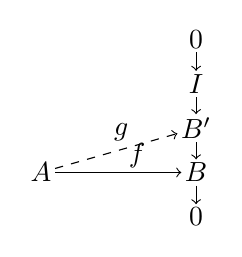
\begin{tikzpicture}[x=1em,y=1em,every node/.style={inner sep=1.1pt}]
  \node (top) at (5,6.4) {$0$};
  \node (ideal) at (5,4.8) {$I$};
  \node (source) at (5,3.2) {$B'$};
  \node (target) at (5,1.6) {$B$};
  \node (bottom) at (5,0) {$0$};
  \node (ring) at (-.6,1.6) {$A$};
  \draw[->] (top)--(ideal);
  \draw[->] (ideal)--(source);
  \draw[->] (source)--(target);
  \draw[->] (target)--(bottom);
  \draw[->,dashed] (ring)--node[pos=.54,above=2pt] {$g$} (source);
  \draw[->] (ring)--node[pos=.65,above=.3pt] {$f$} (target);
\end{tikzpicture}\par
}
\smallskip
\noindent We call this result the \emph{infinitesimal lifting property} for $A$. We prove this result in several steps.

\noindent\hangindent=1.7em (a) First suppose that $g\colon A\to B'$ is a given homomorphism lifting $f$. If $g'\colon A\to B'$ is another such homomorphism, show that $\theta=g-g'$ is a $k$-derivation of $A$ into $I$, which we can consider as an element of $\operatorname{Hom}_A(\Omega_{A/k},I)$. Note that since $I^2=0$, $I$ has a natural structure of $B$-module and hence also of $A$-module. Conversely, for any $\theta\in\operatorname{Hom}_A(\Omega_{A/k},I)$, $g'=g+\theta$ is another homomorphism lifting $f$. (For this step, you do not need the hypothesis about $\operatorname{Spec} A$ being nonsingular.)

\noindent\hangindent=1.7em (b) Now let $P=k[x_1,\ldots,x_n]$ be a polynomial ring over $k$ of which $A$ is a quotient, and let $J$ be the kernel. Show that there does exist a homomorphism $h\colon P\to B'$ making a commutative diagram,\par
{\centering
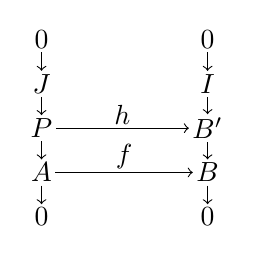
\begin{tikzpicture}[x=1em,y=1em,every node/.style={inner sep=1.1pt}]
  \node (l0) at (0,6.4) {$0$};
  \node (l1) at (0,4.8) {$J$};
  \node (l2) at (0,3.2) {$P$};
  \node (l3) at (0,1.6) {$A$};
  \node (l4) at (0,0) {$0$};
  \node (r0) at (6,6.4) {$0$};
  \node (r1) at (6,4.8) {$I$};
  \node (r2) at (6,3.2) {$B'$};
  \node (r3) at (6,1.6) {$B$};
  \node (r4) at (6,0) {$0$};
  \draw[->] (l0)--(l1);
  \draw[->] (l1)--(l2);
  \draw[->] (l2)--(l3);
  \draw[->] (l3)--(l4);
  \draw[->] (r0)--(r1);
  \draw[->] (r1)--(r2);
  \draw[->] (r2)--(r3);
  \draw[->] (r3)--(r4);
  \draw[->] (l2)--node[above] {$h$} (r2);
  \draw[->] (l3)--node[above] {$f$} (r3);
\end{tikzpicture}\par
}
\noindent\hspace*{1.7em}and show that $h$ induces an $A$-linear map $\bar h\colon J/J^2\to I$.

\noindent\hangindent=1.7em (c) Now use the hypothesis $\operatorname{Spec} A$ nonsingular and (\Goto{result-II-8.17}{8.17}) to obtain an exact sequence
\[
0\longrightarrow J/J^2\longrightarrow\Omega_{P/k}\otimes A\longrightarrow\Omega_{A/k}\longrightarrow0.
\]
Show furthermore that applying the functor $\operatorname{Hom}_A(\cdot,I)$ gives an exact sequence
\[
0\longrightarrow\operatorname{Hom}_A(\Omega_{A/k},I)\longrightarrow
\operatorname{Hom}_P(\Omega_{P/k},I)\longrightarrow\operatorname{Hom}_A(J/J^2,I)\longrightarrow0.
\]
Let $\theta\in\operatorname{Hom}_P(\Omega_{P/k},I)$ be an element whose image gives $\bar h\in\operatorname{Hom}_A(J/J^2,I)$. Consider $\theta$ as a derivation of $P$ to $B'$. Then let $h'=h-\theta$, and show that $h'$ is a homomorphism of $P\to B'$ such that $h'(J)=0$. Thus $h'$ induces the desired homomorphism $g\colon A\to B'$.

\smallskip
\noindent\hypertarget{ex-II-8.7}{}\textbf{8.7.} As an application of the infinitesimal lifting property, we consider the following general problem. Let $X$ be a scheme of finite type over $k$, and let $\mathcal F$ be a coherent sheaf on $X$. We seek to classify schemes $X'$ over $k$, which have a sheaf of ideals $\mathcal I$ such that $\mathcal I^2=0$ and $(X',\mathcal O_{X'}/\mathcal I)\cong(X,\mathcal O_X)$, and such that $\mathcal I$ with its resulting structure of $\mathcal O_X$-module is isomorphic to the given sheaf $\mathcal F$. Such a pair $X',\mathcal I$ we call an \emph{infinitesimal extension} of the scheme $X$ by the sheaf $\mathcal F$. One such}
% Contents from body/page-204.tex.
\BookMark{1}{2.9  Formal Schemes}{sec-II-9}
\ChapterSheet{204}{190}{\Goto{p-74}{II\quad Schemes}}{%
\noindent extension, the \emph{trivial one}, is obtained as follows. Take $\mathcal O_{X'}=\mathcal O_X\oplus\mathcal F$ as sheaves of abelian groups, and define multiplication by $(a\oplus f)\cdot(a'\oplus f')=aa'\oplus(af'+a'f)$. Then the topological space $X$ with the sheaf of rings $\mathcal O_{X'}$ is an infinitesimal extension of $X$ by $\mathcal F$.

The general problem of classifying extensions of $X$ by $\mathcal F$ can be quite complicated. So for now, just prove the following special case: if $X$ is affine and nonsingular, then any extension of $X$ by a coherent sheaf $\mathcal F$ is isomorphic to the trivial one. See (III, Ex.~\Goto{ex-III-4.10}{4.10}) for another case.

\smallskip
\noindent\hypertarget{ex-II-8.8}{}\textbf{8.8.} Let $X$ be a projective nonsingular variety over $k$. For any $n>0$ we define the $n$th \emph{plurigenus} of $X$ to be $P_n=\dim_k\Gamma(X,\omega_X^{\otimes n})$. Thus in particular $P_1=p_g$. Also, for any $q$, $0\le q\le\dim X$ we define an integer $h^{q,0}=\dim_k\Gamma(X,\Omega_{X/k}^q)$ where $\Omega_{X/k}^q=\bigwedge^q\Omega_{X/k}$ is the sheaf of regular $q$-forms on $X$. In particular, for $q=\dim X$, we recover the geometric genus again. The integers $h^{q,0}$ are called \emph{Hodge numbers}.

Using the method of (\Goto{result-II-8.19}{8.19}), show that $P_n$ and $h^{q,0}$ are \emph{birational invariants} of $X$, i.e., if $X$ and $X'$ are birationally equivalent nonsingular projective varieties, then $P_n(X)=P_n(X')$ and $h^{q,0}(X)=h^{q,0}(X')$.

\medskip
\noindent\hypertarget{sec-II-9}{}{\large\bfseries 9\quad Formal Schemes}\par
\smallskip
One feature which clearly distinguishes the theory of schemes from the older theory of varieties is the possibility of having nilpotent elements in the structure sheaf of a scheme. In particular, if $Y$ is a closed subvariety of a variety $X$, defined by a sheaf of ideals $\mathcal I$, then for any $n\ge1$ we can consider the closed subscheme $Y_n$ defined by the $n$th power $\mathcal I^n$ of the sheaf of ideals $\mathcal I$. \EditionText{If $Y\subsetneq X$ and $n\ge2$, then $Y_n$ has nonzero nilpotent local sections of its structure sheaf.} It carries information about $Y$ together with the infinitesimal properties of the embedding of $Y$ in $X$.

The \emph{formal completion} of $Y$ in $X$, which we will define precisely below, is an object which carries information about all the infinitesimal neighborhoods $Y_n$ of $Y$ at once. Thus it is thicker than any $Y_n$, but it is contained inside any actual open neighborhood of $Y$ in $X$. We might call it the formal neighborhood of $Y$ in $X$.

The idea of considering these formal completions is already implicit in the memoir of Zariski \Goto{bib-483-14}{[3]}, where he uses the \textquotedblleft{}holomorphic functions along a subvariety\textquotedblright{} for his proof of the connectedness principle. We will give different proofs of some of Zariski's results, using cohomology, in (III, \Goto{sec-III-11}{\S11}). A striking application of formal schemes as something in between a subvariety and an ambient variety is in Grothendieck's proof of the Lefschetz theorems on Pic and $\pi_1$ \Goto{bib-SGA-2}{[SGA 2]}. This material is also explained in Hartshorne \Goto{bib-477-6}{[5, Ch.~IV]}.

We will define an arbitrary formal scheme as something which looks locally like the completion of a usual scheme along a closed subscheme.

\medskip
\noindent\emph{Inverse Limits of Abelian Groups}\par
\smallskip
\noindent First we recall the notion of inverse limit. An \emph{inverse system} of abelian groups is a collection of abelian groups $A_n$, for each $n\ge1$, together with}
% Contents from body/page-205.tex.
\ChapterSheet[10.8]{205}{191}{\Goto{sec-II-9}{9\quad Formal Schemes}}{%
\noindent homomorphisms $\varphi_{n'n}\colon A_{n'}\to A_n$ for each $n'\ge n$, such that for each $n''\ge n'\ge n$ we have $\varphi_{n''n}=\varphi_{n'n}\circ\varphi_{n''n'}$\EditionText{, and $\varphi_{nn}=\operatorname{id}_{A_n}$.} We will denote the inverse system by $(A_n,\varphi_{n'n})$, or simply $(A_n)$, with the $\varphi$ being understood. If $(A_n)$ is an inverse system of abelian groups, we define the \emph{inverse limit} $A=\varprojlim A_n$ to be the set of sequences $\{a_n\}\in\prod A_n$ such that $\varphi_{n'n}(a_{n'})=a_n$ for all $n'\ge n$. Clearly $A$ is a group. The inverse limit $A$ can be characterized by the following universal property: given a group $B$, and homomorphisms $\psi_n\colon B\to A_n$ for each $n$, such that for any $n'\ge n$, $\psi_n=\varphi_{n'n}\circ\psi_{n'}$, then there exists a unique homomorphism $\psi\colon B\to A$ such that $\psi_n=p_n\circ\psi$ for each $n$, where $p_n\colon A\to A_n$ is the restriction of the $n$th projection map $\prod A_n\to A_n$.

If the groups $A_n$ have the additional structure of vector spaces over a field $k$, or modules over a ring $R$, then the above discussion makes sense in the category of $k$-vector spaces or $R$-modules.

\smallskip
Next we study exactness properties of the inverse limit (cf.\ Atiyah--Macdonald \Goto{legacy-b-am}{[1, Ch.~10]}). A \emph{homomorphism} $(A_n)\to(B_n)$ of inverse systems of abelian groups is a collection of homomorphisms $f_n\colon A_n\to B_n$ for each $n$, which are compatible with the maps of the inverse system, i.e., for each $n'\ge n$, we have a commutative diagram\par
{\centering
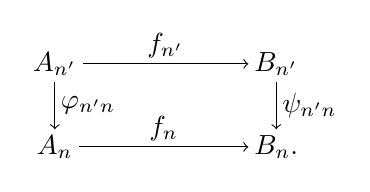
\begin{tikzpicture}[x=1em,y=1em,every node/.style={inner sep=2pt}]
  \node (ul) at (0,3) {$A_{n'}$};
  \node (ur) at (8,3) {$B_{n'}$};
  \node (dl) at (0,0) {$A_n$};
  \node (dr) at (8,0) {$B_n$.};
  \draw[->] (ul)--node[above] {$f_{n'}$} (ur);
  \draw[->] (dl)--node[above] {$f_n$} (dr);
  \draw[->] (ul)--node[right] {$\varphi_{n'n}$} (dl);
  \draw[->] (ur)--node[right] {$\psi_{n'n}$} (dr);
\end{tikzpicture}\par
}
\noindent A sequence
\[
0\longrightarrow(A_n)\longrightarrow(B_n)\longrightarrow(C_n)\longrightarrow0
\]
of homomorphisms of inverse systems is \emph{exact} if the corresponding sequence of groups is exact for each $n$. Given such a short exact sequence of inverse systems, one sees easily that the sequence of inverse limits
\[
0\longrightarrow\varprojlim A_n\longrightarrow\varprojlim B_n\longrightarrow\varprojlim C_n
\]
is also exact. However, the last map need not be surjective. So we say that $\varprojlim$ is a left exact functor.

To give a criterion for exactness of $\varprojlim$ on the right, we make the following definition: an inverse system $(A_n,\varphi_{n'n})$ satisfies the \emph{Mittag--Leffler condition} (ML) if for each $n$, the decreasing family $\{\varphi_{n'n}(A_{n'})\subseteq A_n\mid n'\ge n\}$ of subgroups of $A_n$ is stationary. In other words, for each $n$, there is an $n_0\ge n$, such that for all $n',n''\ge n_0$, $\varphi_{n'n}(A_{n'})=\varphi_{n''n}(A_{n''})$ as subgroups of $A_n$.

Suppose an inverse system $(A_n)$ satisfies (ML). Then for each $n$, we let $A_n'\subseteq A_n$ be the \emph{stable image} $\varphi_{n'n}(A_{n'})$ for any $n'\ge n_0$, which exists by the definition. Then one sees easily that $(A_n')$ is also an inverse system, with the induced maps, and that the maps of the new system $(A_n')$ are all surjective. Furthermore, it is clear that $\varprojlim A_n'=\varprojlim A_n$. So we see that $A=\varprojlim A_n$ maps surjectively to each $A_n'$.}
% Contents from body/page-206.tex.
\ChapterSheet{206}{192}{\Goto{p-74}{II\quad Schemes}}{%
\noindent\hypertarget{result-II-9.1}{}\textbf{Proposition 9.1.} \emph{Let}
\[
0\longrightarrow(A_n)\xrightarrow{f}(B_n)\xrightarrow{g}(C_n)\longrightarrow0
\]
\emph{be a short exact sequence of inverse systems of abelian groups. Then:}

\noindent\hspace*{1.7em}\hypertarget{result-II-9.1-a}{}(a) \emph{if $(B_n)$ satisfies (ML), so does $(C_n)$.}

\noindent\hspace*{1.7em}\hypertarget{result-II-9.1-b}{}(b) \emph{if $(A_n)$ satisfies (ML), then the sequence of inverse limits}
\[
0\longrightarrow\varprojlim A_n\longrightarrow\varprojlim B_n\longrightarrow\varprojlim C_n\longrightarrow0
\]
\emph{is exact.}

\smallskip
\noindent\textsc{Proof.} (See also Grothendieck \Goto{bib-EGA}{[EGA~$0_{\mathrm{III}}$, 13.2]}.) 

(a) For each $n'\ge n$, the image of $B_{n'}$ in $B_n$ maps surjectively to the image of $C_{n'}$ in $C_n$, so (ML) for $(B_n)$ implies (ML) for $(C_n)$ immediately.

(b) The only nonobvious part is to show that the last map is surjective. So let $\{c_n\}\in\varprojlim C_n$. For each $n$, let $E_n=g^{-1}(c_n)$. Then $E_n$ is a subset of $B_n$, and $(E_n)$ is an inverse system of sets. Furthermore, each $E_n$ is bijective, in a noncanonical way, with $A_n$, because of the exactness of the sequence $0\to A_n\to B_n\to C_n\to0$. Thus since $(A_n)$ satisfies (ML), one sees easily that $(E_n)$ satisfies the Mittag--Leffler condition as an inverse system of sets (same definition). Since each $E_n$ is nonempty, it follows from considering the inverse system of stable images as above, that $\varprojlim E_n$ is also nonempty. Taking any element of this set gives an element of $\varprojlim B_n$ which maps to $\{c_n\}$.

\smallskip
\noindent\hypertarget{result-II-9.1.1}{}\textbf{Example 9.1.1.} If all the maps $\varphi_{n'n}\colon A_{n'}\to A_n$ are surjective, then $(A_n)$ satisfies (ML), so (\Goto{result-II-9.1-b}{9.1b}) applies.

\smallskip
\noindent\hypertarget{result-II-9.1.2}{}\textbf{Example 9.1.2.} If $(A_n)$ is an inverse system of finite-dimensional vector spaces over a field, or more generally, an inverse system of modules with descending chain condition over a ring, then $(A_n)$ satisfies (ML).

\medskip
\noindent\emph{Inverse Limits of Sheaves}\par
\smallskip
In any category $\mathfrak C$, we define the notion of inverse limit by analogy with the universal property of the inverse limit of abelian groups above. Thus if $(A_n,\varphi_{n'n})$ is an inverse system of objects of $\mathfrak C$ (same definition as above), then an \emph{inverse limit} $A=\varprojlim A_n$ is an object $A$ of $\mathfrak C$, together with morphisms $p_n\colon A\to A_n$ for each $n$, such that for each $n'\ge n$, $p_n=\varphi_{n'n}\circ p_{n'}$, satisfying the following universal property: given any object $B$ of $\mathfrak C$, together with morphisms $\psi_n\colon B\to A_n$ for each $n$, such that for each $n'\ge n$, $\psi_n=\varphi_{n'n}\circ\psi_{n'}$, there exists a unique morphism $\psi\colon B\to A$ such that for each $n$, $\psi_n=p_n\circ\psi$. Clearly the inverse limit is unique if it exists. But the question of existence depends on the particular category considered.

\smallskip
\noindent\hypertarget{result-II-9.2}{}\textbf{Proposition 9.2.} \emph{Let $X$ be a topological space, and let $\mathfrak C$ be the category of sheaves of abelian groups on $X$. Then inverse limits exist in $\mathfrak C$. Furthermore, if $(\mathcal F_n)$ is an inverse system of sheaves on $X$, and $\mathcal F=\varprojlim\mathcal F_n$ is its inverse limit, then for any open set $U$, we have $\Gamma(U,\mathcal F)=\varprojlim\Gamma(U,\mathcal F_n)$ in the category of abelian groups.}}
% Contents from body/page-207.tex.
\ChapterSheet[10.7]{207}{193}{\Goto{sec-II-9}{9\quad Formal Schemes}}{%
\noindent\textsc{Proof.} Given an inverse system of sheaves $(\mathcal F_n)$ on $X$, we consider the presheaf $U\mapsto\varprojlim\Gamma(U,\mathcal F_n)$, where this inverse limit is taken in the category of abelian groups. Now using the sheaf property for each $\mathcal F_n$, one verifies immediately that this presheaf is a sheaf. Call it $\mathcal F$. Now given any other sheaf $\mathcal G$, and a system of compatible maps $\psi_n\colon\mathcal G\to\mathcal F_n$ for each $n$, it follows from the universal property of an inverse limit of abelian groups that we obtain unique maps, for each $U$, $\Gamma(U,\mathcal G)\to\Gamma(U,\mathcal F)$. These give a sheaf map $\mathcal G\to\mathcal F$, thus verifying that $\mathcal F$ is the inverse limit of the $\mathcal F_n$ in $\mathfrak C$.

\smallskip
\noindent\hypertarget{result-II-9.2.1}{}\textbf{Caution 9.2.1.} Even though inverse limits exist in the category $\mathfrak C$ of abelian sheaves on a topological space, one must beware of using intuition derived from the category of abelian groups. In particular, the statement of (\Goto{result-II-9.1-b}{9.1b}) is \emph{false} in $\mathfrak C$, even if all maps in the inverse system $(A_n)$ are surjective. So in studying exactness questions, we will always pass to sections over an open set, and thus reduce to questions about abelian groups. For more details about exactness of $\varprojlim$ in $\mathfrak C$, see Hartshorne \Goto{bib-477-8}{[7, I, \S4]}.

\medskip
\noindent\emph{Completion of a Ring}\par
\smallskip
One important application of inverse limits is to define the completion of a ring with respect to an ideal. This generalizes the notion of completion of a local ring which was discussed in (I, \Goto{sec-I-5}{\S5}). It also forms the algebraic model for the completion of a scheme along a closed subscheme which will come next.

So let $A$ be a commutative ring with identity (as always), and let $I$ be an ideal of $A$. We denote by $I^n$ the $n$th power of the ideal $I$. Then we have natural homomorphisms
\[
\cdots\longrightarrow A/I^3\longrightarrow A/I^2\longrightarrow A/I,
\]
which make $(A/I^n)$ into an inverse system of rings. The inverse limit ring $\varprojlim A/I^n$ is denoted by $\widehat A$ and is called the \emph{completion of $A$ with respect to $I$} or the \emph{$I$-adic completion of $A$}. For each $n$ we have a natural map $A\to A/I^n$, so by the universal property we obtain a homomorphism $A\to\widehat A$.

Similarly, if $M$ is any $A$-module, we define $\widehat M=\varprojlim M/I^nM$, and call it the \emph{$I$-adic completion of $M$}. It has a natural structure of $\widehat A$-module.

\medskip
\noindent\hypertarget{result-II-9.3A}{}\textbf{Theorem 9.3A.} \emph{Let $A$ be a noetherian ring, and $I$ an ideal of $A$. We denote by $\widehat{\vphantom A\ }$ the $I$-adic completion as above. Then:}

\noindent\hspace*{1.7em}\hypertarget{result-II-9.3A-a}{}(a) \emph{$\widehat I=\varprojlim I/I^n$ is an ideal of $\widehat A$. For any $n$, $\widehat I^n=I^n\widehat A$, and $\widehat A/\widehat I^n\cong A/I^n$;}

\noindent\hspace*{1.7em}\hypertarget{result-II-9.3A-b}{}(b) \emph{if $M$ is a finitely generated $A$-module, then $\widehat M\cong M\otimes_A\widehat A$;}

\noindent\hangindent=3em\hspace*{1.7em}\hypertarget{result-II-9.3A-c}{}(c) \emph{the functor $M\mapsto\widehat M$ is an exact functor on the category of finitely generated $A$-modules;}

\noindent\hspace*{1.7em}\hypertarget{result-II-9.3A-d}{}(d) \emph{$\widehat A$ is a noetherian ring;}

\noindent\hangindent=3em\hspace*{1.7em}\hypertarget{result-II-9.3A-e}{}(e) \emph{if $(M_n)$ is an inverse system, where each $M_n$ is a finitely generated $A/I^n$-module, each $\varphi_{n'n}\colon M_{n'}\to M_n$ is surjective, and $\ker\varphi_{n'n}=I^nM_{n'}$, then $M=\varprojlim M_n$ is a finitely generated $\widehat A$-module, and for each $n$, $M_n\cong M/I^nM$.}}
% Contents from body/page-208.tex.
\ChapterSheet{208}{194}{\Goto{p-74}{II\quad Schemes}}{%
\noindent\textsc{Proofs.}

\noindent\hspace*{1.7em}(a) Atiyah--Macdonald \Goto{legacy-b-am}{[1, p.~109]}.

\noindent\hspace*{1.7em}(b) \Goto{legacy-b-am}{[Ibid., p.~108]}.

\noindent\hspace*{1.7em}(c) \Goto{legacy-b-am}{[Ibid., p.~108]}.

\noindent\hspace*{1.7em}(d) \Goto{legacy-b-am}{[Ibid., p.~113]}.

\noindent\hspace*{1.7em}(e) Bourbaki \Goto{bib-474-4-item-1}{[1, Ch.~III, \S2, no.~11, Prop.\ \& Cor.~14]}.

\medskip
\noindent\emph{Formal Schemes}\par
\smallskip
We begin by defining the completion of a scheme along a closed subscheme. For technical reasons we will limit our discussion to noetherian schemes.

\medskip
\noindent\textbf{Definition.} Let $X$ be a noetherian scheme, and let $Y$ be a closed subscheme, defined by a sheaf of ideals $\mathcal I$. Then we define the \emph{formal completion of $X$ along $Y$}, denoted $(\widehat X,\mathcal O_{\widehat X})$, to be the following ringed space. We take the topological space $Y$, and on it the sheaf of rings $\mathcal O_{\widehat X}=\varprojlim\mathcal O_X/\mathcal I^n$. Here we consider each $\mathcal O_X/\mathcal I^n$ as a sheaf of rings on $Y$, and make them into an inverse system in the natural way.

\medskip
\noindent\hypertarget{result-II-9.3.1}{}\textbf{Remark 9.3.1.} The structure sheaf $\mathcal O_{\widehat X}$ of $\widehat X$ actually depends only on the closed subset $Y$, and not on the particular scheme structure on $Y$. For if $\mathcal J$ is another sheaf of ideals defining a closed subscheme structure on $Y$, then since $X$ is a noetherian scheme, there are integers $m,n$ such that $\mathcal I\supseteq\mathcal J^m$ and $\mathcal J\supseteq\mathcal I^n$. Thus the inverse systems $(\mathcal O_X/\mathcal I^n)$ and $(\mathcal O_X/\mathcal J^m)$ are cofinal with each other, and hence have the same inverse limit.

One sees easily that the stalks of the sheaf $\mathcal O_{\widehat X}$ are local rings, so in fact $(\widehat X,\mathcal O_{\widehat X})$ is a locally ringed space. If $U=\operatorname{Spec} A$ is an open affine subset of $X$, and if $I\subseteq A$ is the ideal $\Gamma(U,\mathcal I)$, then from (\Goto{result-II-9.2}{9.2}) we see that $\Gamma(\widehat X\cap U,\mathcal O_{\widehat X})=\widehat A$, the $I$-adic completion of $A$. Thus the process of completing $X$ along $Y$ is analogous to the $I$-adic completion of a ring discussed above. However, one should note that the local rings of $\widehat X$ are in general \emph{not} complete, and \EditionText{the dimension of a local ring of $\widehat X$ need not agree with the dimension of the underlying topological space $Y$.}

\medskip
\noindent\textbf{Definition.} With $X,Y,\mathcal I$ as in the previous definition, let $\mathcal F$ be a coherent sheaf on $X$. We define the \emph{completion of $\mathcal F$ along $Y$}, denoted $\widehat{\mathcal F}$, to be the sheaf $\varprojlim\mathcal F/\mathcal I^n\mathcal F$ on $Y$. It has a natural structure of $\mathcal O_{\widehat X}$-module.

\medskip
\noindent\textbf{Definition.} A \emph{noetherian formal scheme} is a locally ringed space $(\mathfrak X,\mathcal O_{\mathfrak X})$ which has a finite open cover $\{U_i\}$ such that for each $i$, the pair $(U_i,\mathcal O_{\mathfrak X}|_{U_i})$ is isomorphic, as a locally ringed space, to the completion of some noetherian scheme $X_i$ along a closed subscheme $Y_i$. A \emph{morphism} of noetherian formal schemes is a morphism as locally ringed spaces. A sheaf $\mathfrak F$ of $\mathcal O_{\mathfrak X}$-modules is said to be \emph{coherent} if there is a finite open cover $U_i$ as above, with $U_i\cong\widehat X_i$, and for each $i$ there is a coherent sheaf $\mathcal F_i$ on $X_i$ such that $\mathfrak F|_{U_i}\cong\widehat{\mathcal F}_i$ as $\mathcal O_{\widehat X_i}$-modules via the given isomorphism $U_i\cong\widehat X_i$.}
% Contents from body/page-209.tex.
\ChapterSheet{209}{195}{\Goto{sec-II-9}{9\quad Formal Schemes}}{%
\noindent\hypertarget{result-II-9.3.2}{}\textbf{Examples 9.3.2.} If $X$ is any noetherian scheme, and $Y$ a closed subscheme, then its completion $\widehat X$ is a formal scheme. Such a formal scheme, which can be obtained by completing a \emph{single} noetherian scheme along a closed subscheme, is called \emph{algebraizable}. It is not so easy to give examples, but there are nonalgebraizable noetherian formal schemes---see Hironaka and Matsumura \Goto{bib-477-17-item-1}{[1, \S5]} or Hartshorne \Goto{bib-477-6}{[5, V, 3.3, p.~205]}.

\medskip
\noindent\hypertarget{result-II-9.3.3}{}\textbf{Example 9.3.3.} If $X$ is a noetherian scheme, and we take $Y=X$, then $\widehat X=X$. Thus the category of noetherian formal schemes includes all noetherian schemes.

\medskip
\noindent\hypertarget{result-II-9.3.4}{}\textbf{Example 9.3.4.} If $X$ is a noetherian scheme, and $Y$ is a closed point $P$, then $\widehat X$ is a one point space $\{P\}$ with the completion $\widehat{\mathcal O}_P$ of the local ring at $P$ as its structure sheaf. An $\widehat{\mathcal O}_P$-module $M$, considered as a sheaf on $\widehat X$, is coherent if and only if $M$ is a finitely generated module. Indeed, clearly coherent implies finitely generated. But the converse is also true since we can obtain $\widehat X$ by completing the scheme $\operatorname{Spec}\widehat{\mathcal O}_P$ at its closed point, and any finitely generated $\widehat{\mathcal O}_P$-module $M$ corresponds to a coherent sheaf on $\operatorname{Spec}\widehat{\mathcal O}_P$.

\smallskip
Next we will study the structure of coherent sheaves on a formal scheme. As in the study of coherent sheaves on usual schemes in \Goto{sec-II-5}{\S5}, we first analyze what happens in the affine case.

\medskip
\noindent\textbf{Definition.} An \emph{affine (noetherian) formal scheme} is a formal scheme obtained by completing a single affine noetherian scheme along a closed subscheme. If $X=\operatorname{Spec} A$, $Y=V(I)$, and $\mathfrak X=\widehat X$, then for any finitely generated $A$-module $M$, we define the sheaf $M^\triangle$ on $\mathfrak X$ to be the completion of the coherent sheaf $\widetilde M$ on $X$. Thus by definition, $M^\triangle$ is a coherent sheaf on $\mathfrak X$.

\medskip
\noindent\hypertarget{result-II-9.4}{}\textbf{Proposition 9.4.} \emph{Let $A$ be a noetherian ring, $I$ an ideal of $A$, let $X=\operatorname{Spec} A$, $Y=V(I)$, and let $\mathfrak X=\widehat X$. Then:}

\noindent\hangindent=3em\hspace*{1.7em}\hypertarget{result-II-9.4-a}{}(a) \emph{$\mathfrak J=I^\triangle$ is a sheaf of ideals in $\mathcal O_{\mathfrak X}$, and for any $n$, $\mathcal O_{\mathfrak X}/\mathfrak J^n\cong(A/I^n)^\sim$ as sheaves on $Y$;}

\noindent\hangindent=3em\hspace*{1.7em}\hypertarget{result-II-9.4-b}{}(b) \emph{if $M$ is a finitely generated $A$-module, then $M^\triangle=\widetilde M\otimes_{\mathcal O_X}\mathcal O_{\mathfrak X}$.}

\noindent\hangindent=3em\hspace*{1.7em}\hypertarget{result-II-9.4-c}{}(c) \emph{The functor $M\mapsto M^\triangle$ is an exact functor from the category of finitely generated $A$-modules to the category of coherent $\mathcal O_{\mathfrak X}$-modules.}

\smallskip
\noindent\textsc{Proof.} In each case we have a statement about sheaves on $\mathfrak X$. Since the open affine subsets of $X$ form a base for the topology of $X$, and their intersections with $Y$ a base for the topology of $Y$, it will be sufficient to establish the corresponding property of the sections over any such open set. So let $U=\operatorname{Spec} B$ be an open affine subset of $X$, let $J=\Gamma(U,\widetilde I)$, and for any finitely generated $A$-module $M$, let $N=\Gamma(U,\widetilde M)$. Then $B$ is a noetherian ring (\Goto{result-II-3.2}{3.2}), $N$ is a finitely generated $B$-module (\Goto{result-II-5.4}{5.4}), and the functor $M\mapsto N$ is an exact functor from $A$-modules to $B$-modules (\Goto{result-II-5.5}{5.5}).}
% Contents from body/page-210.tex.
\ChapterSheet{210}{196}{\Goto{p-74}{II\quad Schemes}}{%
We prove \Goto{result-II-9.4-c}{(c)} first. So let $M$ be a finitely generated $A$-module. Then $M^\triangle=\varprojlim\widetilde M/\widetilde I^{\,n}\widetilde M$ by definition, so by (\Goto{result-II-9.2}{9.2}), $\Gamma(U,M^\triangle)=\varprojlim\Gamma(U,\widetilde M/\widetilde I^{\,n}\widetilde M)$. But this is equal to $\varprojlim N/J^nN=\widehat N$, where $\widehat{\vphantom A\ }$ now denotes the $J$-adic completion of a $B$-module. Now $M\mapsto N$ is exact as we saw above, and $N\mapsto\widehat N$ is exact by (\Goto{result-II-9.3A}{9.3A}). Thus $M\mapsto\Gamma(U,M^\triangle)$ is exact for each $U$, and so $M\mapsto M^\triangle$ is exact.

(a) For any $U$ as above, $\Gamma(U,I^\triangle)=\varprojlim\Gamma(U,\widetilde I/\widetilde I^{\,n})=\widehat J$. Furthermore $\Gamma(U,\mathcal O_{\mathfrak X})=\widehat B$ similarly. But by (\Goto{result-II-9.3A}{9.3A}), $\widehat J$ is an ideal of $\widehat B$, so this shows that $\mathfrak J=I^\triangle$ is a sheaf of ideals in $\mathcal O_{\mathfrak X}$.

Now we consider the exact sequence of $A$-modules
\[
0\longrightarrow I^n\longrightarrow A\longrightarrow A/I^n\longrightarrow0.
\]
According to \Goto{result-II-9.4-c}{(c)} which we have already proved, this gives an exact sequence of $\mathcal O_{\mathfrak X}$-modules
\[
0\longrightarrow\mathfrak J^n\longrightarrow\mathcal O_{\mathfrak X}\longrightarrow(A/I^n)^\triangle\longrightarrow0.
\]
Observe that the inverse system which defines $(A/I^n)^\triangle$ as the completion of $(A/I^n)^\sim$ is eventually stationary, since this sheaf is annihilated by $\widetilde I^{\,n}$. Hence $(A/I^n)^\triangle=(A/I^n)^\sim$, and we conclude that $\mathcal O_{\mathfrak X}/\mathfrak J^n\cong(A/I^n)^\sim$ as required.

(b) We have a slight abuse of notation in our statement: since $\widetilde M$ and $\mathcal O_X$ are sheaves on $X$, we should actually write $M^\triangle\cong\widetilde M|_Y\otimes_{\mathcal O_X|_Y}\mathcal O_{\mathfrak X}$. But we will simply regard $M^\triangle$ and $\mathcal O_{\mathfrak X}$ as sheaves on $X$, by extending by zero outside of $Y$ (Ex.~\Goto{ex-II-1.19}{1.19}). For any finitely generated $A$-module $M$, and for $U$ an open set as above, we have $\Gamma(U,M^\triangle)=\widehat N$ as before. On the other hand, $\widetilde M\otimes_{\mathcal O_X}\mathcal O_{\mathfrak X}$ is the sheaf associated to the presheaf
\[
U\mapsto\Gamma(U,\widetilde M)\otimes_{\Gamma(U,\mathcal O_X)}\Gamma(U,\mathcal O_{\mathfrak X})=N\otimes_B\widehat B.
\]
Since $\widehat N\cong N\otimes_B\widehat B$ by (\Goto{result-II-9.3A}{9.3A}), we conclude that the corresponding sheaves are isomorphic too: $M^\triangle\cong\widetilde M\otimes_{\mathcal O_X}\mathcal O_{\mathfrak X}$.

\medskip
\noindent\textbf{Definition.} Let $(\mathfrak X,\mathcal O_{\mathfrak X})$ be a noetherian formal scheme. A sheaf of ideals $\mathfrak J\subseteq\mathcal O_{\mathfrak X}$ is called an \emph{ideal of definition for $\mathfrak X$} if $\operatorname{Supp}\mathcal O_{\mathfrak X}/\mathfrak J=\mathfrak X$ and the locally ringed space $(\mathfrak X,\mathcal O_{\mathfrak X}/\mathfrak J)$ is a noetherian scheme.

\medskip
\noindent\hypertarget{result-II-9.5}{}\textbf{Proposition 9.5.} \emph{Let $(\mathfrak X,\mathcal O_{\mathfrak X})$ be a noetherian formal scheme.}

\noindent\hangindent=3em\hspace*{1.7em}\hypertarget{result-II-9.5-a}{}(a) \emph{If $\mathfrak J_1$ and $\mathfrak J_2$ are two ideals of definition, then there are integers $m,n>0$ such that $\mathfrak J_1\supseteq\mathfrak J_2^m$ and $\mathfrak J_2\supseteq\mathfrak J_1^n$.}

\noindent\hangindent=3em\hspace*{1.7em}\hypertarget{result-II-9.5-b}{}(b) \emph{There is a unique largest ideal of definition $\mathfrak J$, characterized by the fact that $(\mathfrak X,\mathcal O_{\mathfrak X}/\mathfrak J)$ is a reduced scheme. In particular, ideals of definition exist.}

\noindent\hangindent=3em\hspace*{1.7em}\hypertarget{result-II-9.5-c}{}(c) \emph{If $\mathfrak J$ is an ideal of definition, so is $\mathfrak J^n$, for any $n>0$.}

\smallskip
\noindent\textsc{Proof.}

(a) Let $\mathfrak J_1$ and $\mathfrak J_2$ be two ideals of definition. Then on the topological space $\mathfrak X$, we have surjective maps of sheaves of rings $f_1\colon\mathcal O_{\mathfrak X}\to\mathcal O_{\mathfrak X}/\mathfrak J_1$ and $f_2\colon\mathcal O_{\mathfrak X}\to\mathcal O_{\mathfrak X}/\mathfrak J_2$. For any point $P\in\mathfrak X$, the stalk $(\mathfrak J_2)_P$ of $\mathfrak J_2$ at $P$ is contained}
% Contents from body/page-211.tex.
\ChapterSheet[10.4]{211}{197}{\Goto{sec-II-9}{9\quad Formal Schemes}}{%
\noindent in $\mathfrak m_P$, the maximal ideal of the local ring $\mathcal O_{\mathfrak X,P}$. Indeed, $\mathcal O_{\mathfrak X,P}/(\mathfrak J_2)_P$ is the local ring of $P$ on the scheme $(\mathfrak X,\mathcal O_{\mathfrak X}/\mathfrak J_2)$. In particular, it is nonzero, so $(\mathfrak J_2)_P\subseteq\mathfrak m_P$. Now we consider the sheaf of ideals $f_1(\mathfrak J_2)$ on the scheme $(\mathfrak X,\mathcal O_{\mathfrak X}/\mathfrak J_1)$. For each point $P$, its stalk is contained inside the maximal ideal of the local ring. Hence every local section of $f_1(\mathfrak J_2)$ is nilpotent (Ex.~\Goto{ex-II-2.18}{2.18}), and since $(\mathfrak X,\mathcal O_{\mathfrak X}/\mathfrak J_1)$ is a noetherian scheme, $f_1(\mathfrak J_2)$ itself is nilpotent. This shows that for some $m>0$, $\mathfrak J_1\supseteq\mathfrak J_2^m$. The other way follows by symmetry.

(b) Suppose $(\mathfrak X,\mathcal O_{\mathfrak X}/\mathfrak J_1)$ is a reduced scheme. Then in the proof of \Goto{result-II-9.5-a}{(a)}, we find $f_1(\mathfrak J_2)=0$, so $\mathfrak J_1\supseteq\mathfrak J_2$. Thus such a $\mathfrak J_1$ is largest, if it exists. Since it is unique, the existence becomes a local question. Thus we may assume that $\mathfrak X$ is the completion of an affine noetherian scheme $X$ along a closed subscheme $Y$. By (\Goto{result-II-9.3.1}{9.3.1}) we may assume that $Y$ has the reduced induced structure. Let $X=\operatorname{Spec} A$, $Y=V(I)$. Then by (\Goto{result-II-9.4}{9.4}), $\mathfrak J=I^\triangle$ is an ideal in $\mathcal O_{\mathfrak X}$, and $\mathcal O_{\mathfrak X}/\mathfrak J\cong(A/I)^\sim=\mathcal O_Y$. Thus $\mathfrak J$ is an ideal of definition for which $(\mathfrak X,\mathcal O_{\mathfrak X}/\mathfrak J)$ is reduced. This shows the existence of the largest ideal of definition.

(c) Let $\mathfrak J$ be any ideal of definition, and suppose given $n>0$. Let $\mathfrak J_0$ be the unique largest ideal of definition. Then by \Goto{result-II-9.5-a}{(a)}, there is an integer $r$ such that $\mathfrak J\supseteq\mathfrak J_0^r$, and hence $\mathfrak J^n\supseteq\mathfrak J_0^{nr}$. First note that $\mathfrak J_0^{nr}$ is an ideal of definition. Indeed, this can be checked locally. If $\mathfrak J_0=I^\triangle$ on an affine, using the notation of \Goto{result-II-9.5-b}{(b)}, then $\mathcal O_{\mathfrak X}/\mathfrak J_0^{nr}\cong(A/I^{nr})^\sim$ by (\Goto{result-II-9.4}{9.4}), so $(\mathfrak X,\mathcal O_{\mathfrak X}/\mathfrak J_0^{nr})$ is a scheme with support $Y$. Let's call this scheme $Y'$, and let $f\colon\mathcal O_{\mathfrak X}\to\mathcal O_{Y'}$ be the corresponding map of sheaves. Then $(Y',\mathcal O_{Y'}/f(\mathfrak J))=(\mathfrak X,\mathcal O_{\mathfrak X}/\mathfrak J)$ is a noetherian scheme, by hypothesis, so $f(\mathfrak J)$ is a coherent sheaf. Therefore $f(\mathfrak J^n)=f(\mathfrak J)^n$ is also coherent, and we conclude that $(Y',\mathcal O_{Y'}/f(\mathfrak J^n))=(\mathfrak X,\mathcal O_{\mathfrak X}/\mathfrak J^n)$ is also a noetherian scheme.

\medskip
\noindent\hypertarget{result-II-9.6}{}\textbf{Proposition 9.6.} \emph{Let $\mathfrak X$ be a noetherian formal scheme and let $\mathfrak J$ be an ideal of definition. For each $n>0$ we denote by $Y_n$ the scheme $(\mathfrak X,\mathcal O_{\mathfrak X}/\mathfrak J^n)$.}

\noindent\hangindent=3em\hspace*{1.7em}\hypertarget{result-II-9.6-a}{}(a) \emph{If $\mathfrak F$ is a coherent sheaf of $\mathcal O_{\mathfrak X}$-modules, then for each $n$, $\mathcal F_n=\mathfrak F/\mathfrak J^n\mathfrak F$ is a coherent sheaf of $\mathcal O_{Y_n}$-modules, and $\mathfrak F\cong\varprojlim\mathcal F_n$.}

\noindent\hangindent=3em\hspace*{1.7em}\hypertarget{result-II-9.6-b}{}(b) \emph{Conversely, suppose given for each $n$ a coherent $\mathcal O_{Y_n}$-module $\mathcal F_n$, together with surjective maps $\varphi_{n'n}\colon\mathcal F_{n'}\to\mathcal F_n$, for each $n'\ge n$, making $\{\mathcal F_n\}$ into an inverse system of sheaves. Assume furthermore that for each $n'\ge n$, $\ker\varphi_{n'n}=\mathfrak J^n\mathcal F_{n'}$. Then $\mathfrak F=\varprojlim\mathcal F_n$ is a coherent $\mathcal O_{\mathfrak X}$-module, and for each $n$, $\mathcal F_n\cong\mathfrak F/\mathfrak J^n\mathfrak F$.}

\smallskip
\noindent\textsc{Proof.}

\EditionText{Locally write $\mathfrak X$ as the completion of $\operatorname{Spec} A$ along $V(I)$ and take $A$ to be $I$-adically complete. By (\Goto{result-II-9.5}{9.5}), $(I^\triangle)^s\subseteq\mathfrak J$ for some $s$. The ideal $\mathfrak J/(I^\triangle)^s$ on $\operatorname{Spec}(A/I^s)$ comes from an ideal $J/I^s$. By (\Goto{result-II-9.4-c}{9.4c}), $J^\triangle=\mathfrak J$. The two adic filtrations are cofinal by (\Goto{result-II-9.5}{9.5}) and (\Goto{result-II-9.4-a}{9.4a}), so the same affine presentation uses $J$, with $Y_n=\operatorname{Spec}(A/J^n)$.\par}
(a) \EditionText{Write $\mathfrak F=M^\triangle$ for a finitely generated $A$-module $M$. As in the proof of (\Goto{result-II-9.4-a}{9.4a}), $\mathfrak F/\mathfrak J^n\mathfrak F\cong(M/J^nM)^\sim$. Thus $\mathcal F_n$ is coherent on $Y_n$, and $\mathfrak F\cong\varprojlim\mathcal F_n$.}

(b) \EditionText{}For each $n$, let $M_n=\Gamma(Y_n,\mathcal F_n)$. Then}
% Contents from body/page-212.tex.
\ChapterSheet{212}{198}{\Goto{p-74}{II\quad Schemes}}{%
\noindent $(M_n)$ is an inverse system of modules satisfying the hypotheses of (\Goto{result-II-9.3A-e}{9.3Ae}). Therefore we conclude that $M=\varprojlim M_n$ is a finitely generated $A$-module (since $A$ is complete), and that for each $n$, $M_n\cong M/\EditionText{J}^nM$. But then $\mathfrak F=\varprojlim\mathcal F_n$ is just $M^\triangle$, hence it is a coherent $\mathcal O_{\mathfrak X}$-module. Furthermore $\mathfrak F/\mathfrak J^n\mathfrak F\cong(M/\EditionText{J}^nM)^\sim$ as in \Goto{result-II-9.6-a}{(a)}, so $\mathfrak F/\mathfrak J^n\mathfrak F\cong\mathcal F_n$.

\medskip
\noindent\hypertarget{result-II-9.7}{}\textbf{Theorem 9.7.} \emph{Let $A$ be a noetherian ring, $I$ an ideal, and assume that $A$ is $I$-adically complete. Let $X=\operatorname{Spec} A$, $Y=V(I)$, and $\mathfrak X=\widehat X$. Then the functors $M\mapsto M^\triangle$ and $\mathfrak F\mapsto\Gamma(\mathfrak X,\mathfrak F)$ are exact, and inverse to each other, on the categories of finitely generated $A$-modules and coherent $\mathcal O_{\mathfrak X}$-modules respectively. Thus they establish an equivalence of categories. In particular, every coherent $\mathcal O_{\mathfrak X}$-module $\mathfrak F$ is of the form $M^\triangle$ for some $M$.}

\smallskip
\noindent\textsc{Proof.} We have already seen that $M\mapsto M^\triangle$ is exact (\Goto{result-II-9.4}{9.4}). If $M$ is an $A$-module of finite type, then $\Gamma(\mathfrak X,M^\triangle)=\varprojlim M/I^nM=\widehat M$, and $\widehat M=M$ because $A$ is complete (\Goto{result-II-9.3A-b}{9.3Ab}). Thus one composition of our two functors is the identity.

Conversely, let $\mathfrak F$ be a coherent $\mathcal O_{\mathfrak X}$-module, and let $\mathfrak J=I^\triangle$. Then by (\Goto{result-II-9.6-a}{9.6a}), $\mathfrak F\cong\varprojlim\mathcal F_n$, where for each $n>0$, $\mathcal F_n=\mathfrak F/\mathfrak J^n\mathfrak F$. Now the inverse system of sheaves $(\mathcal F_n)$ satisfies the hypotheses of (\Goto{result-II-9.6-b}{9.6b}), and the proof of (\Goto{result-II-9.6-b}{9.6b}) shows in fact that $\mathfrak F\cong M^\triangle$, for some finitely generated $A$-module $M$. Furthermore, by (\Goto{result-II-9.2}{9.2}), $\Gamma(\mathfrak X,\mathfrak F)=\varprojlim\Gamma(Y,(M/I^nM)^\sim)=\varprojlim M/I^nM=\widehat M$, which is equal to $M$ since $A$ is complete. This shows that $\Gamma(\mathfrak X,\mathfrak F)$ is a finitely generated $A$-module, and $\mathfrak F\cong\Gamma(\mathfrak X,\mathfrak F)^\triangle$. Thus the other composition of our two functors is the identity.

It remains to show that the functor $\Gamma(\mathfrak X,\cdot)$ is exact on the category of coherent $\mathcal O_{\mathfrak X}$-modules. So let
\[
0\longrightarrow\mathfrak F_1\longrightarrow\mathfrak F_2\longrightarrow\mathfrak F_3\longrightarrow0
\]
be an exact sequence of coherent $\mathcal O_{\mathfrak X}$-modules. For each $i$, let $M_i=\Gamma(\mathfrak X,\mathfrak F_i)$. Then the $M_i$ are finitely generated $A$-modules, and we have at least a left-exact sequence
\[
0\longrightarrow M_1\longrightarrow M_2\longrightarrow M_3.
\]
Let $R$ be the cokernel on the right. Then applying the functor $\triangle$ we obtain an exact sequence
\[
0\longrightarrow M_1^\triangle\longrightarrow M_2^\triangle\longrightarrow M_3^\triangle\longrightarrow R^\triangle\longrightarrow0
\]
on $\mathfrak X$. But for each $i$, $M_i^\triangle\cong\mathfrak F_i$ as we saw above, so we conclude that $R^\triangle=0$. But also by the above, $R=\Gamma(\mathfrak X,R^\triangle)$, so $R=0$. This shows that $\Gamma(\mathfrak X,\cdot)$ is exact, which concludes the proof.

\medskip
\noindent\hypertarget{result-II-9.8}{}\textbf{Corollary 9.8.} \emph{If $X$ is any noetherian scheme, $Y$ a closed subscheme, and $\mathfrak X=\widehat X$ the completion along $Y$, then the functor $\mathcal F\mapsto\widehat{\mathcal F}$ is an exact functor from coherent $\mathcal O_X$-modules to coherent $\mathcal O_{\mathfrak X}$-modules. Furthermore, if $\mathcal I$ is the sheaf of ideals of $Y$, and $\widehat{\mathcal I}$ its completion, then we have $\widehat{\mathcal F}/\widehat{\mathcal I}^{\,n}\widehat{\mathcal F}\cong\mathcal F/\mathcal I^n\mathcal F$ for each $n$, and $\widehat{\mathcal F}\cong\mathcal F\otimes_{\mathcal O_X}\mathcal O_{\mathfrak X}$.}}
% Contents from body/page-213.tex.
\ChapterSheet[10.6]{213}{199}{\Goto{sec-II-9}{9\quad Formal Schemes}}{%
\noindent\textsc{Proof.} These questions are all local, in which case they reduce to (\Goto{result-II-9.4}{9.4}).

\medskip
\noindent\hypertarget{result-II-9.9}{}\textbf{Corollary 9.9.} \emph{Any kernel, cokernel, or image of a morphism of coherent sheaves on a noetherian formal scheme is again coherent.}

\smallskip
\noindent\textsc{Proof.} These questions are also local, in which case they follow from (\Goto{result-II-9.7}{9.7}).

\medskip
\noindent\hypertarget{result-II-9.9.1}{}\textbf{Remark 9.9.1.} It is also true that an extension of coherent sheaves on a noetherian formal scheme is coherent (Ex.~\Goto{ex-II-9.4}{9.4}). On the other hand, some properties of coherent sheaves on usual schemes do not carry over to formal schemes. For example, if $\mathfrak X$ is the completion of a projective variety $X\subseteq\mathbf P_k^n$ along a closed subvariety $Y$, and if $\mathcal O_{\mathfrak X}(1)=\mathcal O_X(1)^\wedge$, then there may be nonzero coherent sheaves $\mathfrak F$ on $\mathfrak X$ such that $\Gamma(\mathfrak X,\mathfrak F(v))=0$ for all $v\in\mathbb Z$. In particular, no twist of $\mathfrak F$ is generated by global sections (III, Ex.~\Goto{ex-III-11.7}{11.7}).

\medskip
\noindent\textsc{Exercises}

\smallskip
\noindent\hypertarget{ex-II-9.1}{}\textbf{9.1.} Let $X$ be a noetherian scheme, $Y$ a closed subscheme, and $\widehat X$ the completion of $X$ along $Y$. We call the ring $\Gamma(\widehat X,\mathcal O_{\widehat X})$ the ring of \emph{formal-regular functions} on $X$ along $Y$. In this exercise we show that if $Y$ is a connected, nonsingular, positive-dimensional subvariety of $X=\mathbf P_k^n$ over an algebraically closed field $k$, then $\Gamma(\widehat X,\mathcal O_{\widehat X})=k$.

\noindent\hangindent=3em\hspace*{1.7em}(a) Let $\mathcal I$ be the ideal sheaf of $Y$. Use (\Goto{result-II-8.13}{8.13}) and (\Goto{result-II-8.17}{8.17}) to show that there is an inclusion of sheaves on $Y$, $\mathcal I/\mathcal I^2\hookrightarrow\mathcal O_Y(-1)^{n+1}$.

\noindent\hangindent=3em\hspace*{1.7em}(b) Show that for any $r\ge1$, $\Gamma(Y,\mathcal I^r/\mathcal I^{r+1})=0$.

\noindent\hangindent=3em\hspace*{1.7em}(c) Use the exact sequences
\[
0\longrightarrow\mathcal I^r/\mathcal I^{r+1}\longrightarrow\mathcal O_X/\mathcal I^{r+1}\longrightarrow\mathcal O_X/\mathcal I^r\longrightarrow0
\]
and induction on $r$ to show that $\Gamma(Y,\mathcal O_X/\mathcal I^r)=k$ for all $r\ge1$. (Use (\Goto{result-II-8.21A}{8.21Ae}).)

\noindent\hangindent=3em\hspace*{1.7em}(d) Conclude that $\Gamma(\widehat X,\mathcal O_{\widehat X})=k$. (Actually, the same result holds without the hypothesis $Y$ nonsingular, but the proof is more difficult---see Hartshorne \Goto{bib-477-4}{[3, (7.3)]}.)

\smallskip
\noindent\hypertarget{ex-II-9.2}{}\textbf{9.2.} Use the result of (Ex.~\Goto{ex-II-9.1}{9.1}) to prove the following geometric result. Let $Y\subseteq X=\mathbf P_k^n$ be as above, and let $f\colon X\to Z$ be a morphism of $k$-varieties. Suppose that $f(Y)$ is a single closed point $P\in Z$. Then $f(X)=P$ also.

\smallskip
\noindent\hypertarget{ex-II-9.3}{}\textbf{9.3.} Prove the analogue of (\Goto{result-II-5.6}{5.6}) for formal schemes, which says, if $\mathfrak X$ is an affine formal scheme, and if
\[
0\longrightarrow\mathfrak F'\longrightarrow\mathfrak F\longrightarrow\mathfrak F''\longrightarrow0
\]
is an exact sequence of $\mathcal O_{\mathfrak X}$-modules, and if $\mathfrak F'$ is coherent, then the sequence of global sections
\[
0\longrightarrow\Gamma(\mathfrak X,\mathfrak F')\longrightarrow\Gamma(\mathfrak X,\mathfrak F)\longrightarrow\Gamma(\mathfrak X,\mathfrak F'')\longrightarrow0
\]
is exact. For the proof, proceed in the following steps.

\noindent\hangindent=3em\hspace*{1.7em}(a) Let $\mathfrak J$ be an ideal of definition for $\mathfrak X$, and for each $n>0$ consider the exact sequence
\[
0\longrightarrow\mathfrak F'/\mathfrak J^n\mathfrak F'\longrightarrow\mathfrak F/\mathfrak J^n\mathfrak F'\longrightarrow\mathfrak F''\longrightarrow0.
\]}
% Contents from body/page-214.tex.
\ChapterSheet{214}{200}{\Goto{p-74}{II\quad Schemes}}{%
\noindent\hangindent=3em\hspace*{3em}Use (\Goto{result-II-5.6}{5.6}), slightly modified, to show that for every open affine subset $\mathfrak U\subseteq\mathfrak X$, the sequence
\[
0\longrightarrow\Gamma(\mathfrak U,\mathfrak F'/\mathfrak J^n\mathfrak F')\longrightarrow\Gamma(\mathfrak U,\mathfrak F/\mathfrak J^n\mathfrak F')\longrightarrow\Gamma(\mathfrak U,\mathfrak F'')\longrightarrow0
\]
is exact.

\noindent\hangindent=3em\hspace*{1.7em}(b) Now pass to the limit, using (\Goto{result-II-9.1}{9.1}), (\Goto{result-II-9.2}{9.2}), and (\Goto{result-II-9.6}{9.6}). Conclude that $\mathfrak F\cong\varprojlim\mathfrak F/\mathfrak J^n\mathfrak F'$ and that the sequence of global sections above is exact.

\smallskip
\noindent\hypertarget{ex-II-9.4}{}\textbf{9.4.} Use (Ex.~\Goto{ex-II-9.3}{9.3}) to prove that if
\[
0\longrightarrow\mathfrak F'\longrightarrow\mathfrak F\longrightarrow\mathfrak F''\longrightarrow0
\]
is an exact sequence of $\mathcal O_{\mathfrak X}$-modules on a noetherian formal scheme $\mathfrak X$, and if $\mathfrak F',\mathfrak F''$ are coherent, then $\mathfrak F$ is coherent also.

\smallskip
\noindent\hypertarget{ex-II-9.5}{}\textbf{9.5.} If $\mathfrak F$ is a coherent sheaf on a noetherian formal scheme $\mathfrak X$, which can be generated by global sections, show in fact that it can be generated by a finite number of its global sections.

\smallskip
\noindent\hypertarget{ex-II-9.6}{}\textbf{9.6.} Let $\mathfrak X$ be a noetherian formal scheme, let $\mathfrak J$ be an ideal of definition, and for each $n$, let $Y_n$ be the scheme $(\mathfrak X,\mathcal O_{\mathfrak X}/\mathfrak J^n)$. Assume that the inverse system of groups $(\Gamma(Y_n,\mathcal O_{Y_n}))$ satisfies the Mittag--Leffler condition. Then prove that $\operatorname{Pic}\mathfrak X=\varprojlim\operatorname{Pic}Y_n$. As in the case of a scheme, we define $\operatorname{Pic}\mathfrak X$ to be the group of locally free $\mathcal O_{\mathfrak X}$-modules of rank $1$ under the operation $\otimes$. Proceed in the following steps.

\noindent\hangindent=3em\hspace*{1.7em}(a) \EditionText{Use that the thickenings have the same underlying space and that the restriction map on structure sheaves has nilpotent kernel. Invertibility of a section is then detected by restriction. Use this} to show that the inverse system $(\Gamma(Y_n,\mathcal O_{Y_n}^*))$ of units in the respective rings also satisfies (ML).

\noindent\hangindent=3em\hspace*{1.7em}(b) Let $\mathfrak F$ be a coherent sheaf of $\mathcal O_{\mathfrak X}$-modules, and assume that for each $n$, there is some isomorphism $\varphi_n\colon\mathfrak F/\mathfrak J^n\mathfrak F\cong\mathcal O_{Y_n}$. Then show that there is an isomorphism $\mathfrak F\cong\mathcal O_{\mathfrak X}$. Be careful, because the $\varphi_n$ may not be compatible with the maps in the two inverse systems $(\mathfrak F/\mathfrak J^n\mathfrak F)$ and $(\mathcal O_{Y_n})$! Conclude that the natural map $\operatorname{Pic}\mathfrak X\to\varprojlim\operatorname{Pic}Y_n$ is injective.

\noindent\hangindent=3em\hspace*{1.7em}(c) Given an invertible sheaf $\mathcal L_n$ on $Y_n$ for each $n$, and given isomorphisms $\mathcal L_{n+1}\otimes\mathcal O_{Y_n}\cong\mathcal L_n$, construct maps $\mathcal L_{n'}\to\mathcal L_n$ for each $n'\ge n$ so as to make an inverse system, and show that $\mathcal L=\varprojlim\mathcal L_n$ is a coherent sheaf on $\mathfrak X$. Then show that $\mathcal L$ is locally free of rank $1$, and thus conclude that the map $\operatorname{Pic}\mathfrak X\to\varprojlim\operatorname{Pic}Y_n$ is surjective. Again be careful, because even though each $\mathcal L_n$ is locally free of rank $1$, the open sets needed to make them free might get smaller and smaller with $n$.

\noindent\hangindent=3em\hspace*{1.7em}(d) Show that the hypothesis \textquotedblleft{}$(\Gamma(Y_n,\mathcal O_{Y_n}))$ satisfies (ML)\textquotedblright{} is satisfied if either $\mathfrak X$ is affine, or each $Y_n$ is projective over a field $k$.

\noindent\hspace*{3em}\emph{Note:} See (III, Ex.~\Goto{ex-III-11.5}{11.5}--\Goto{ex-III-11.7}{11.7}) for further examples and applications.}
